% ===========================================================================
%  Aprendizado de Mundo Aberto em Poços de Petróleo
%  Da detecção baseada em regras à explicabilidade por agentes de linguagem
%
%  Compilação:  latexmk -pdf main.tex
%           ou:  pdflatex main -> bibtex main -> makeindex main -> pdflatex x2
% ===========================================================================
\documentclass[11pt,a4paper,twoside,openright]{book}

% ---------------------------------------------------------------------------
% Preâmbulo comum do livro
% ---------------------------------------------------------------------------

% --- Codificação e idioma ---------------------------------------------------
\usepackage[T1]{fontenc}
\usepackage[utf8]{inputenc}
\usepackage[brazil]{babel}
\usepackage{lmodern}
\usepackage{microtype}

% --- Matemática -------------------------------------------------------------
\usepackage{amsmath}
\usepackage{amssymb}
\usepackage{amsfonts}
\usepackage{mathtools}
\usepackage{bm}

% --- Tabelas e figuras ------------------------------------------------------
\usepackage{graphicx}
\usepackage{epstopdf}
\epstopdfsetup{update,prepend}
\usepackage{booktabs}
\usepackage{longtable}
\usepackage{multirow}
\usepackage{array}
\usepackage{tabularx}
\usepackage{rotating}
\usepackage[font=small,labelfont=bf]{caption}
\usepackage{subcaption}
\usepackage{float}

% --- Cores e caixas ---------------------------------------------------------
\usepackage{xcolor}
\usepackage[most]{tcolorbox}
\tcbuselibrary{skins,breakable}

% --- Listagens de código ----------------------------------------------------
\usepackage{listings}
\definecolor{codfundo}{RGB}{247,247,247}
\definecolor{codcomentario}{RGB}{100,120,100}
\definecolor{codpalavra}{RGB}{20,60,140}
\definecolor{codtexto}{RGB}{150,60,40}
\lstdefinestyle{python}{
  language         = Python,
  basicstyle       = \ttfamily\footnotesize,
  keywordstyle     = \color{codpalavra}\bfseries,
  commentstyle     = \color{codcomentario}\itshape,
  stringstyle      = \color{codtexto},
  numbers          = none,
  showstringspaces = false,
  breaklines       = true,
  breakatwhitespace= true,
  columns          = fullflexible,
  backgroundcolor  = \color{codfundo},
  frame            = single,
  rulecolor        = \color{black!25},
  framesep         = 5pt,
  xleftmargin      = 5pt,
  xrightmargin     = 5pt,
  aboveskip        = 1.1em,
  belowskip        = 1.1em,
  literate         = {á}{{\'a}}1 {ã}{{\~a}}1 {ç}{{\c c}}1 {é}{{\'e}}1
                     {ê}{{\^e}}1 {í}{{\'i}}1 {ó}{{\'o}}1 {õ}{{\~o}}1 {ú}{{\'u}}1
}
\lstset{style=python}

% --- Unidades e números -----------------------------------------------------
\usepackage{siunitx}
\sisetup{
  output-decimal-marker = {,},
  group-separator       = {.},
  group-minimum-digits  = 4,
  detect-weight         = true,
  detect-family         = true
}

% --- Layout -----------------------------------------------------------------
\usepackage[a4paper,inner=3cm,outer=2.5cm,top=3cm,bottom=2.5cm]{geometry}
\usepackage{emptypage}
\usepackage{enumitem}
% Evita o aviso "Negative labelwidth" nas listas de descricao com leftmargin=0pt
\setlist[description]{labelwidth=0pt,labelsep=0pt}
\usepackage{makeidx}
\makeindex

% --- Bibliografia -----------------------------------------------------------
\usepackage[round,authoryear]{natbib}
\bibliographystyle{apalike}
\renewcommand{\bibname}{Referências}

% --- Hyperref e referências cruzadas (carregar por último) ------------------
\usepackage[hidelinks,breaklinks=true]{hyperref}
\hypersetup{
  pdftitle  = {Aprendizado de Mundo Aberto em Poços de Petróleo},
  pdfauthor = {Lucas Gouveia Omena Lopes},
  pdfsubject= {Detecção, classificação e explicação de anomalias em poços de petróleo},
  pdfkeywords = {mundo aberto, detecção de anomalias, poços de petróleo, aprendizado profundo, LLM}
}
\usepackage[brazilian]{cleveref}

% ---------------------------------------------------------------------------
% Nomes em português para o cleveref
% ---------------------------------------------------------------------------
\crefname{chapter}{Capítulo}{Capítulos}
\Crefname{chapter}{Capítulo}{Capítulos}
\crefname{part}{Parte}{Partes}
\Crefname{part}{Parte}{Partes}
\crefname{section}{Seção}{Seções}
\Crefname{section}{Seção}{Seções}
\crefname{figure}{Figura}{Figuras}
\Crefname{figure}{Figura}{Figuras}
\crefname{table}{Tabela}{Tabelas}
\Crefname{table}{Tabela}{Tabelas}
\crefname{equation}{Equação}{Equações}
\Crefname{equation}{Equação}{Equações}

% ---------------------------------------------------------------------------
% Ambientes didáticos
% ---------------------------------------------------------------------------
\definecolor{corDefinicao}{HTML}{1F4E79}
\definecolor{corExemplo}{HTML}{2E7D32}
\definecolor{corDestaque}{HTML}{B35C00}
\definecolor{corExercicio}{HTML}{5B2C6F}
\definecolor{corResultado}{HTML}{8B1A1A}

\newtcolorbox[auto counter,number within=chapter]{definicao}[2][]{%
  breakable, enhanced, colback=corDefinicao!4, colframe=corDefinicao,
  fonttitle=\bfseries, title={Definição~\thetcbcounter\ --- #2}, #1}

\newtcolorbox[auto counter,number within=chapter]{exemplo}[2][]{%
  breakable, enhanced, colback=corExemplo!4, colframe=corExemplo,
  fonttitle=\bfseries, title={Exemplo~\thetcbcounter\ --- #2}, #1}

\newtcolorbox{destaque}[1][Em resumo]{%
  breakable, enhanced, colback=corDestaque!5, colframe=corDestaque,
  fonttitle=\bfseries, title={#1}}

\newtcolorbox{resultadochave}[1][Resultado-chave]{%
  breakable, enhanced, colback=corResultado!4, colframe=corResultado,
  fonttitle=\bfseries, title={#1}}

\newtcolorbox{objetivos}{%
  breakable, enhanced, colback=black!3, colframe=black!55,
  fonttitle=\bfseries, title={Objetivos de aprendizagem}}

\newenvironment{exercicios}%
  {\section*{Exercícios}\addcontentsline{toc}{section}{Exercícios}%
   \begin{enumerate}[label=\textbf{\arabic*.},leftmargin=*,itemsep=0.4em]}%
  {\end{enumerate}}

\newenvironment{leituras}%
  {\section*{Leituras recomendadas}\addcontentsline{toc}{section}{Leituras recomendadas}%
   \begin{itemize}[leftmargin=*,itemsep=0.3em]}%
  {\end{itemize}}

\newcommand{\resumocapitulo}[1]{%
  \section*{Resumo do capítulo}\addcontentsline{toc}{section}{Resumo do capítulo}#1}

% ---------------------------------------------------------------------------
% Macros de notação
% ---------------------------------------------------------------------------
\newcommand{\vect}[1]{\bm{#1}}
\newcommand{\mat}[1]{\bm{#1}}
\newcommand{\R}{\mathbb{R}}
\newcommand{\E}{\mathbb{E}}
\newcommand{\prob}{\mathbb{P}}
\DeclareMathOperator*{\argmax}{arg\,max}
\DeclareMathOperator*{\argmin}{arg\,min}
\DeclareMathOperator{\std}{std}

% Primeira ocorrência de termo estrangeiro
\newcommand{\ing}[1]{\emph{#1}}
% Termo em português seguido do original em inglês
\newcommand{\termo}[2]{#1\index{#1}\ (\ing{#2})}

% Siglas frequentes
\newcommand{\treW}{3W}


\graphicspath{{figuras/}}

\begin{document}

% ---------------------------------------------------------------------------
\frontmatter
% ---------------------------------------------------------------------------

\begin{titlepage}
\centering
\vspace*{3cm}
{\Huge\bfseries Aprendizado de Mundo Aberto\\[0.4em] em Poços de Petróleo\par}
\vspace{1.2cm}
{\Large Da detecção baseada em regras à explicabilidade\\ por agentes de linguagem\par}
\vspace{3cm}
{\Large\bfseries Lucas Gouveia Omena Lopes\par}
\vspace{0.6cm}
{\large Thales Miranda de Almeida Vieira\par}
{\large Eduardo Toledo de Lima Junior\par}
{\large William Wagner Matos Lira\par}
\vspace{0.6cm}
{\large Pedro Esteves Aranha\par}
{\large Ricardo Emanuel Vaz Vargas\par}
\vfill
{\large Laboratório de Computação Científica e Visualização\\
Universidade Federal de Alagoas\par}
\vspace{0.4cm}
{\large Petrobras\par}
\vspace{0.8cm}
{\large Maceió --- 2026\par}
\end{titlepage}

\cleardoublepage
\chapter*{Prefácio}
\addcontentsline{toc}{chapter}{Prefácio}
\markboth{Prefácio}{Prefácio}

Este livro conta a história de uma ideia.

A ideia é simples de enunciar e difícil de realizar: \emph{um sistema de monitoramento
industrial não deveria fingir que já viu tudo}. Quando um poço de petróleo a dois mil
metros de lâmina d'água começa a se comportar de forma estranha, o classificador que
o vigia tem duas escolhas honestas --- dizer ``isto é um fechamento espúrio da válvula
de segurança'' ou dizer ``isto eu nunca vi''. O que ele não deveria fazer, e no entanto
é exatamente o que a maioria dos classificadores faz, é forçar o evento desconhecido
para dentro da categoria conhecida mais próxima e reportar alta confiança.

Essa patologia tem nome. Chama-se \termo{hipótese de mundo fechado}{closed-world
assumption}, e é uma consequência direta da forma como treinamos modelos de
classificação: apresentamos um conjunto finito de classes, otimizamos uma função de
perda que exige que a soma das probabilidades seja igual a um, e obtemos um modelo
que, por construção, é incapaz de responder ``nenhuma das anteriores''. Em um
laboratório isso é uma curiosidade metodológica. Em uma plataforma de produção, é um
alarme que não toca.

\section*{De onde vem este livro}

O material aqui reunido nasceu de uma linha de pesquisa desenvolvida no Laboratório de
Computação Científica e Visualização da Universidade Federal de Alagoas, em cooperação
com a Petrobras, e se organiza em cinco trabalhos encadeados:

\begin{enumerate}[leftmargin=*,itemsep=0.4em]
  \item Um \textbf{sistema dual} que combina um diagrama de decisão baseado em regras
        com um autoencoder recorrente, implantado em mais de vinte unidades flutuantes
        de produção e mais de duzentos e cinquenta poços submarinos. É a prova de que
        o problema é real e de que uma solução híbrida funciona em campo.
  \item Um \textbf{ensemble de classificadores binários} um-contra-todos, que troca a
        pergunta ``qual das nove classes é esta?'' pela pergunta ``esta é a classe
        $k$, sim ou não?'', repetida nove vezes. A mudança parece cosmética; não é.
        É o que permite a resposta ``nenhuma das classes treinadas''.
  \item Uma \textbf{estratégia completa de aprendizado de mundo aberto}, que fecha o
        ciclo: detectar, classificar o que é conhecido, agrupar o que não é, submeter
        os agrupamentos a um especialista e reincorporar as novas classes ao sistema.
  \item Uma \textbf{evolução metodológica} em duas frentes --- da detecção por erro de
        reconstrução para a segmentação temporal supervisionada, e da detecção de
        novidade por ensemble para a detecção por distância de Mahalanobis no espaço
        latente.
  \item Uma \textbf{camada de agente de linguagem}, colocada a jusante de todo o
        restante, cuja função não é classificar melhor, mas explicar, questionar e
        nomear.
\end{enumerate}

Cada um desses trabalhos existe como tese ou artigo. O que faltava era o fio que os
liga --- a narrativa que mostra por que cada passo foi dado, o que exatamente estava
quebrado antes dele e o que continuou quebrado depois. Este livro é esse fio.

\section*{Para quem foi escrito}

Escrevemos para estudantes de pós-graduação e engenheiros que precisam construir --- e
não apenas usar --- sistemas de monitoramento inteligente. Isso impõe duas obrigações.

A primeira é \textbf{não pressupor conhecimento prévio}. Os \cref{cap:introducao} a
\cref{cap:novidades} constroem, do zero, tudo o que é necessário: o vocabulário de
poços e completação, a estrutura dos dados de séries temporais, as métricas de
avaliação em cenários desbalanceados, as arquiteturas de redes recorrentes e
convolucionais, os autoencoders e o conceito de espaço latente, os algoritmos de
agrupamento e os fundamentos de reconhecimento em conjunto aberto. Quem já domina
esse material pode saltar diretamente para a \cref{parte:base}; quem não domina não
ficará para trás.

A segunda obrigação é \textbf{mostrar os números}. Um livro sobre métodos aplicados
que não apresenta resultados não é um livro sobre métodos aplicados. Todas as tabelas
de desempenho dos trabalhos originais são reproduzidas aqui, com discussão crítica ---
inclusive, e sobretudo, dos casos em que o método falhou. A classe \emph{Instabilidade
de Fluxo} atravessa este livro inteiro como um problema não resolvido; a classe
\emph{Hidrato na Linha de Serviço} idem. Preferimos expor essas fronteiras a
escondê-las.

\section*{Uma observação sobre linguagem}

O livro é escrito em português. A terminologia técnica da área, contudo, é
majoritariamente anglófona, e traduzir siglas consagradas seria um desserviço a quem
precisa ler a literatura primária ou conversar com um fornecedor. Adotamos a seguinte
convenção: conceitos são traduzidos, com o termo original em itálico entre parênteses
na primeira ocorrência; siglas operacionais (PDG, TPT, DHSV, ICV, BSW) e nomes de
arquiteturas (LSTM, U-Net) permanecem em inglês, expandidos na primeira ocorrência e
listados na \hyperref[cap:siglas]{lista de siglas}.

Números decimais usam vírgula, conforme a norma brasileira. Quando reproduzimos uma
tabela de um trabalho original em inglês, os valores são convertidos, mas jamais
alterados.

\vspace{1.5em}
\noindent\hfill\emph{Os autores}\\
\noindent\hfill\emph{Maceió, 2026}

\cleardoublepage
\chapter*{Como ler este livro}
\addcontentsline{toc}{chapter}{Como ler este livro}
\markboth{Como ler este livro}{Como ler este livro}

\section*{A arquitetura do argumento}

O livro está organizado em cinco partes que correspondem a cinco momentos de uma
mesma investigação, e a estrutura cabe em um parágrafo.
A Parte~I ensina o necessário. A Parte~II apresenta a base --- três
estratégias que, juntas, constituem o primeiro sistema completo de aprendizado de
mundo aberto para poços de petróleo. A Parte~III mostra como essa base foi revista
quando suas limitações ficaram claras. A Parte~IV acrescenta a camada que faltava:
explicação. A Parte~V amarra tudo e discute o que falta.

\section*{Trilhas de leitura}

\begin{description}[leftmargin=0pt,style=nextline,itemsep=0.7em]

\item[Leitura completa (curso de um semestre).]
Capítulos 1 a 18 na ordem. Os \cref{cap:introducao,cap:dominio,cap:dados} cobrem
domínio e dados; \cref{cap:aprendizado,cap:profundo,cap:novidades} cobrem método;
os demais são aplicação. Uma disciplina de quinze semanas comporta um capítulo por
semana com três semanas de folga para os projetos.

\item[Leitura para quem já sabe aprendizado de máquina.]
Comece pelo \cref{cap:dominio} (o vocabulário de poços é indispensável e não é óbvio),
leia o \cref{cap:dados} (o conjunto 3W tem particularidades que confundem quem chega
de outros domínios), passe rapidamente pelo \cref{cap:novidades} e vá para a
\cref{parte:base}.

\item[Leitura para quem quer implantar.]
\cref{cap:dominio}, \cref{cap:dual} (o sistema que efetivamente está em campo),
\cref{cap:sintese} (arquitetura de referência) e \cref{cap:operacao} (implantação,
deriva, governança). Volte aos demais conforme a necessidade.

\item[Leitura para quem só quer os resultados.]
\cref{cap:dual}, \cref{cap:binarios}, \cref{cap:mundoaberto},
\cref{cap:segmentacao}, \cref{cap:mahalanobis} e \cref{cap:resultados-agente}
contêm todas as tabelas. O \cref{cap:sintese} consolida.

\end{description}

\section*{Convenções tipográficas}

Ao longo do texto você encontrará seis elementos recorrentes.

\begin{objetivos}
Abre cada capítulo. Lista, em forma de verbos de ação, o que se espera que o leitor
saiba fazer ao terminá-lo. Os verbos foram escolhidos para refletir o que o texto de
fato entrega: este é um livro de argumentação e evidência, não um manual de
implementação. Onde o objetivo é ``descrever'' ou ``reconhecer'', o capítulo não
pretende habilitar o leitor a implementar o método do zero; para isso, o
\cref{cap:pratica} aponta código executável e o \cref{cap:reproducao} reúne os
hiperparâmetros.
\end{objetivos}

\medskip
\noindent
As \textbf{caixas de definição}, em azul, introduzem conceitos formais e são numeradas
por capítulo (por exemplo, \emph{Definição 6.2}), de modo que podem ser referenciadas
cruzadamente. As \textbf{caixas de exemplo}, em verde, aplicam o conceito imediatamente
anterior a um caso concreto, quase sempre extraído dos dados reais discutidos no livro,
e seguem a mesma numeração.

\begin{resultadochave}
Destaca um número ou achado que sustenta o argumento do capítulo. É o que você deve
levar consigo se ler apenas as caixas.
\end{resultadochave}

\begin{destaque}[Caixa de atenção]
Marca uma armadilha conceitual, uma limitação relevante ou uma decisão de projeto cuja
motivação não é evidente.
\end{destaque}

\medskip
\noindent
Cada capítulo termina com um \textbf{resumo}, uma lista de \textbf{exercícios} ---
mesclando questões conceituais, exercícios de cálculo e propostas de implementação ---
e sugestões de \textbf{leituras recomendadas}.


\section*{Nomenclatura das classes de anomalia}

Todo o livro utiliza a numeração canônica do conjunto de dados 3W, apresentada em
detalhe no \cref{cap:dados}. Por conveniência, ela é reproduzida aqui:

\begin{center}
\small
\begin{tabular}{cl}
\toprule
\textbf{Classe} & \textbf{Evento} \\
\midrule
0 & Estado normal \\
1 & Aumento abrupto de BSW \\
2 & Fechamento espúrio da DHSV \\
3 & Golfadas severas \\
4 & Instabilidade de fluxo \\
5 & Perda rápida de produtividade \\
6 & Restrição rápida no PCK \\
7 & Incrustação no PCK \\
8 & Hidrato na linha de produção \\
9 & Hidrato na linha de serviço \\
\midrule
--- & Falha de ICV \emph{(dado proprietário; não pertence ao 3W)} \\
--- & Operação de válvula \emph{(dado proprietário; não pertence ao 3W)} \\
\bottomrule
\end{tabular}
\end{center}

\section*{Sobre reprodutibilidade}

O conjunto de dados 3W é público. Os dados proprietários de poços da Petrobras
utilizados nos estudos de caso não o são, e portanto os resultados que dependem
exclusivamente deles não podem ser reproduzidos por terceiros. Sempre que um resultado
depende de dados fechados, isso é dito explicitamente. O \cref{cap:reproducao} reúne
hiperparâmetros, ambiente computacional e procedimentos de avaliação de todos os
experimentos discutidos.

O leitor que quiser executar código, e não apenas lê-lo, deve começar pelo
\cref{cap:pratica}. Ele descreve um recurso didático público, hospedado no próprio
repositório do 3W \citep{Petrobras3W,Lopes2026Intro3W}, que percorre em cinco cadernos
Jupyter todo o caminho da \cref{parte:fundamentos}: tratamento de dados, visualização,
autoencoders, classificadores supervisionados e agrupamento. As caixas de
\textbf{prática} espalhadas pela \cref{parte:fundamentos} apontam, capítulo a capítulo,
qual caderno exercita qual conceito.


\cleardoublepage
\tableofcontents
\cleardoublepage
\listoffigures
\cleardoublepage
\listoftables

\cleardoublepage
\chapter*{Lista de siglas}
\label{cap:siglas}
\addcontentsline{toc}{chapter}{Lista de siglas}
\markboth{Lista de siglas}{Lista de siglas}

\section*{Operação de poços}

\begin{description}[leftmargin=3.6cm,style=nextline,font=\normalfont\bfseries,itemsep=0.15em]
\item[ANM] Árvore de Natal Molhada --- conjunto de válvulas instalado na cabeça do
      poço submarino (\ing{wet christmas tree}).
\item[BSW] \ing{Basic Sediment and Water} --- fração de água e sedimentos no fluido
      produzido.
\item[CKGL] \ing{Gas-Lift Choke} --- válvula reguladora da injeção de gás de elevação.
\item[CKP] \ing{Production Choke} --- válvula reguladora de produção.
\item[DHSV] \ing{Downhole Safety Valve} --- válvula de segurança de subsuperfície.
\item[FPSO] \ing{Floating Production, Storage and Offloading} --- unidade flutuante de
      produção, armazenamento e transferência.
\item[GLV] \ing{Gas-Lift Valve} --- válvula de gás de elevação.
\item[ICV] \ing{Interval Control Valve} --- válvula de controle de intervalo, usada em
      completação inteligente.
\item[M1, M2] Válvulas mestre da árvore de natal.
\item[NPT] \ing{Non-Productive Time} --- tempo não produtivo.
\item[PCK] \ing{Production Choke} --- ver CKP. Nas classes do 3W, designa a região da
      válvula reguladora de produção.
\item[PDG] \ing{Permanent Downhole Gauge} --- sensor permanente de fundo de poço.
\item[PT] \ing{Pressure Transducer} --- transdutor de pressão.
\item[PXO] \ing{Production Cross-Over} --- válvula de cruzamento de produção.
\item[TPT] \ing{Temperature and Pressure Transducer} --- transdutor de temperatura e
      pressão.
\item[WAG] \ing{Water-Alternating-Gas} --- injeção alternada de água e gás.
\item[XO] \ing{Cross-Over} --- válvula de cruzamento.
\end{description}

\section*{Aprendizado de máquina e estatística}

\begin{description}[leftmargin=3.6cm,style=nextline,font=\normalfont\bfseries,itemsep=0.15em]
\item[ACC] Acurácia (\ing{accuracy}).
\item[AE] Autoencoder (\ing{autoencoder}).
\item[ARI] \ing{Adjusted Rand Index} --- índice de Rand ajustado.
\item[CNN] Rede neural convolucional (\ing{convolutional neural network}).
\item[DBSCAN] \ing{Density-Based Spatial Clustering of Applications with Noise}.
\item[DCN] \ing{Deep Clustering Network} --- rede de agrupamento profundo.
\item[GRU] \ing{Gated Recurrent Unit} --- unidade recorrente com portas.
\item[IOU] \ing{Intersection over Union} --- razão entre interseção e união.
\item[LSTM] \ing{Long Short-Term Memory} --- memória de curto prazo longa.
\item[MLP] \ing{Multilayer Perceptron} --- perceptron de múltiplas camadas.
\item[MoE] \ing{Mixture of Experts} --- mistura de especialistas.
\item[MTS] \ing{Multivariate Time Series} --- série temporal multivariada.
\item[OCSVM] \ing{One-Class Support Vector Machine} --- máquina de vetores de suporte
      de uma classe.
\item[OSR] \ing{Open-Set Recognition} --- reconhecimento em conjunto aberto.
\item[OVA] \ing{One-vs-All} --- um-contra-todos.
\item[OWL] \ing{Open-World Learning} --- aprendizado de mundo aberto.
\item[PCA] \ing{Principal Component Analysis} --- análise de componentes principais.
\item[RNN] Rede neural recorrente (\ing{recurrent neural network}).
\item[SMAPE] \ing{Symmetric Mean Absolute Percentage Error} --- erro percentual
      absoluto médio simétrico.
\item[SoftED] \ing{Soft Event Detection} --- família de métricas com tolerância
      temporal para detecção de eventos.
\item[SVM] \ing{Support Vector Machine} --- máquina de vetores de suporte.
\item[t-SNE] \ing{t-Distributed Stochastic Neighbor Embedding}.
\item[UMAP] \ing{Uniform Manifold Approximation and Projection}.
\item[VAE] \ing{Variational Autoencoder} --- autoencoder variacional.
\end{description}

\section*{Modelos de linguagem}

\begin{description}[leftmargin=3.6cm,style=nextline,font=\normalfont\bfseries,itemsep=0.15em]
\item[API] \ing{Application Programming Interface} --- interface de programação de
      aplicações.
\item[CoT] \ing{Chain-of-Thought} --- cadeia de raciocínio.
\item[JSON] \ing{JavaScript Object Notation} --- formato de intercâmbio de dados.
\item[LLM] \ing{Large Language Model} --- modelo de linguagem de grande porte.
\item[NIM] \ing{NVIDIA Inference Microservice} --- serviço de inferência da NVIDIA.
\item[XAI] \ing{Explainable Artificial Intelligence} --- inteligência artificial
      explicável.
\end{description}

\section*{Conjuntos de dados e instituições}

\begin{description}[leftmargin=3.6cm,style=nextline,font=\normalfont\bfseries,itemsep=0.15em]
\item[3W] Conjunto de dados público de eventos indesejáveis reais em poços de
      petróleo, mantido pela Petrobras.
\item[LCCV] Laboratório de Computação Científica e Visualização, UFAL.
\item[OTC] \ing{Offshore Technology Conference}.
\item[SPE] \ing{Society of Petroleum Engineers}.
\item[UFAL] Universidade Federal de Alagoas.
\end{description}

\cleardoublepage
\chapter*{Notação}
\label{cap:notacao-front}
\addcontentsline{toc}{chapter}{Notação}
\markboth{Notação}{Notação}

A notação a seguir é usada de forma consistente em todo o livro. Onde um trabalho
original empregava símbolo diferente, ele foi harmonizado; a correspondência está
registrada no \cref{cap:notacao}.

\section*{Convenções gerais}

\begin{center}
\begin{tabular}{ll}
\toprule
\textbf{Forma} & \textbf{Significado} \\
\midrule
$x$, $\alpha$              & escalar \\
$\vect{x}$                 & vetor (coluna, em negrito) \\
$\mat{X}$, $\mat{\Sigma}$  & matriz (em negrito maiúsculo) \\
$\vect{x}^{\top}$          & transposto \\
$\mat{\Sigma}^{-1}$        & inversa \\
$\|\vect{x}\|$             & norma euclidiana \\
$\hat{y}$                  & valor predito \\
$\bar{x}$                  & média amostral \\
$\R^{d}$                   & espaço euclidiano de dimensão $d$ \\
\bottomrule
\end{tabular}
\end{center}

\section*{Dados e séries temporais}

\begin{center}
\begin{tabular}{ll}
\toprule
\textbf{Símbolo} & \textbf{Significado} \\
\midrule
$T$              & número de passos de tempo de uma janela \\
$S$              & número de sensores (canais) \\
$\mat{X} \in \R^{T \times S}$ & janela multivariada de sensores \\
$\vect{x}_t \in \R^{S}$       & leitura de todos os sensores no instante $t$ \\
$y \in \{0,1,\dots,9\}$       & rótulo de classe do 3W \\
$\mathcal{K}$    & conjunto de classes conhecidas \\
$\mathcal{U}$    & conjunto de classes desconhecidas (novidades) \\
$\vect{b}$       & janela de linha de base, anterior ao evento \\
$\vect{e}$       & janela de evento \\
\bottomrule
\end{tabular}
\end{center}

\section*{Modelos}

\begin{center}
\begin{tabular}{ll}
\toprule
\textbf{Símbolo} & \textbf{Significado} \\
\midrule
$f_{\theta}$     & modelo com parâmetros $\theta$ \\
$g_{\phi}$       & codificador (\ing{encoder}) do autoencoder \\
$h_{\psi}$       & decodificador (\ing{decoder}) do autoencoder \\
$\vect{z} = g_{\phi}(\mat{X}) \in \R^{d}$ & representação latente \\
$d$              & dimensão do espaço latente \\
$\hat{\mat{X}} = h_{\psi}(\vect{z})$ & reconstrução \\
$c_k$            & classificador binário da classe $k$ \\
$s_k \in [0,1]$  & escore do classificador binário $c_k$ \\
$\tau$           & limiar de decisão \\
\bottomrule
\end{tabular}
\end{center}

\section*{Estatística e avaliação}

\begin{center}
\begin{tabular}{ll}
\toprule
\textbf{Símbolo} & \textbf{Significado} \\
\midrule
$\mu$, $\sigma$    & média e desvio-padrão \\
$\mat{\Sigma}$     & matriz de covariância \\
$d_M(\vect{x})$    & distância de Mahalanobis \\
$\lambda$          & parâmetro de regularização da covariância \\
$k$                & multiplicador de desvio-padrão em limiares $\mu + k\sigma$ \\
$K$                & número de agrupamentos (\ing{clusters}) \\
VP, VN             & verdadeiros positivos e verdadeiros negativos \\
FP, FN             & falsos positivos e falsos negativos \\
$\text{ACC}$, $\text{ACC}_b$ & acurácia e acurácia balanceada \\
$\text{REC}$, $\text{PR}$, $\text{SP}$ & revocação, precisão e especificidade \\
$F_1$              & medida F1 \\
\bottomrule
\end{tabular}
\end{center}

\begin{destaque}[Colisão de símbolos]
Dois usos de $k$ convivem no livro e não podem ser confundidos: o \emph{multiplicador
de desvio-padrão} em limiares da forma $\mu + k\sigma$ (\cref{cap:dual},
\cref{cap:mundoaberto}) e o \emph{número de vizinhos ou de posições em um
\ing{ranking}} nas métricas ``top-$k$'' (\cref{cap:resultados-agente}). O contexto
sempre desambigua; quando houver risco, o significado é repetido por extenso.
Da mesma forma, $K$ maiúsculo designa exclusivamente o número de agrupamentos.
\end{destaque}


% ---------------------------------------------------------------------------
\mainmatter
% ---------------------------------------------------------------------------

\part{Fundamentos}\label{parte:fundamentos}
\chapter{Por que vigiar um poço de petróleo}
\label{cap:introducao}

\begin{objetivos}
Ao final deste capítulo, você será capaz de:
\begin{itemize}[leftmargin=*,itemsep=0.2em]
  \item explicar por que a operação de poços submarinos exige monitoramento contínuo e
        automatizado, em termos de segurança, integridade e economia;
  \item quantificar o impacto do tempo não produtivo (NPT) e relacioná-lo à detecção
        precoce de anomalias;
  \item distinguir os três problemas computacionais envolvidos --- detecção,
        classificação e explicação --- e enunciar por que eles não são o mesmo problema;
  \item enunciar a hipótese de mundo fechado e reconhecer suas manifestações práticas;
  \item descrever o percurso argumentativo do livro e escolher a trilha de leitura
        adequada ao seu objetivo.
\end{itemize}
\end{objetivos}

\section{Um poço é um sistema que você não pode ver}

A engenharia costuma lidar com sistemas que podem ser inspecionados. Uma ponte pode
ser percorrida a pé; um vaso de pressão pode ser ensaiado por ultrassom; uma turbina
pode ser aberta. Um poço submarino de petróleo em lâmina d'água de dois mil metros não
pode ser nada disso. Entre o operador na sala de controle e o reservatório a seis mil
metros abaixo da linha d'água existem, no melhor dos casos, algumas dezenas de canais
de telemetria --- pressões, temperaturas, vazões --- amostrados a cada poucos segundos.

Tudo o que se sabe sobre o estado do poço vem desses canais. Se um deles congela, se
um transdutor deriva, se um evento se manifesta em uma escala temporal mais lenta do
que a janela de observação do operador, a observação pode ficar ausente, enviesada ou
insuficiente para identificar o estado. A
consequência é direta: \emph{o monitoramento de poços é, antes de tudo, um problema de
inferência a partir de observação parcial}, uma das classes de problema em que o
aprendizado de máquina pode ser útil.

\subsection{A escala do problema}

Uma única unidade flutuante de produção, armazenamento e transferência (FPSO) pode
estar conectada a algumas dezenas de poços produtores e injetores. Uma operadora de
porte médio opera dezenas de FPSOs. O sistema descrito no \cref{cap:dual} deste livro
foi implantado, à época de sua avaliação, em mais de vinte unidades e mais de duzentos
e cinquenta poços submarinos nas bacias de Santos e de Campos.

Multiplique: se cada poço fornece cinco sinais amostrados a cada segundo, duzentos e
cinquenta poços produzem mais de cem milhões de leituras por dia. Nenhuma equipe de
operação lê cem milhões de números por dia. O que se lê, na prática, são alarmes --- e
alarmes são decisões automatizadas. A qualidade do monitoramento é, portanto, a
qualidade dos algoritmos que decidem quando tocar um alarme.

\subsection{O que dá errado}
\label{sec:introducao-oquedaerrado}

Os eventos indesejáveis que acometem poços de petróleo formam uma taxonomia razoavelmente
estável, detalhada no \cref{cap:dominio}. Por ora, quatro exemplos bastam para dar
concretude ao problema:

\begin{itemize}[leftmargin=*,itemsep=0.4em]
  \item \textbf{Formação de hidratos.} Em águas profundas, a combinação de alta pressão
        e baixa temperatura leva moléculas de água e gás leve a formar um sólido
        cristalino semelhante a gelo. Um tampão de hidrato pode obstruir completamente
        uma linha de produção. A remoção exige despressurização controlada, injeção de
        inibidor ou intervenção submarina, com custo que se mede em milhões de dólares e
        prazo que se mede em semanas.
  \item \textbf{Fechamento espúrio da válvula de segurança de subsuperfície (DHSV).}
        A DHSV é o dispositivo que fecha o poço em situação de emergência. Quando ela
        fecha sem que haja emergência --- por perda de pressão hidráulica na linha de
        controle, por exemplo --- a produção é interrompida. Não é um evento perigoso;
        é um evento caro, e sua reabertura exige diagnóstico correto.
  \item \textbf{Golfadas severas.} O escoamento multifásico em um \ing{riser} vertical
        pode entrar em regime oscilatório de grande amplitude, em que golfadas de
        líquido e bolhas de gás se alternam. O resultado são oscilações de pressão que
        castigam equipamentos de superfície e degradam a eficiência de separação.
  \item \textbf{Incrustação na válvula reguladora de produção (PCK).} Depósitos
        minerais reduzem gradualmente a área de passagem. O sintoma é lento, cumulativo
        e facilmente confundido com declínio natural do reservatório.
\end{itemize}

Observe a heterogeneidade. O hidrato é um evento de horas; a incrustação, de meses. O
fechamento de DHSV é uma transição quase instantânea; a golfada é um regime
estacionário oscilatório. Um método que detecte bem um deles não detectará
necessariamente bem os outros --- e essa observação, que parece trivial aqui, será a
justificativa técnica para praticamente todas as escolhas de arquitetura discutidas
neste livro.

\section{O custo de não saber}

\begin{definicao}{Tempo não produtivo}
Chama-se \termo{tempo não produtivo}{non-productive time} (NPT) o intervalo em que um
poço, sonda ou instalação está indisponível para sua função por causa não planejada.
O NPT é contabilizado em horas ou dias e convertido em custo pela soma do custo de
oportunidade da produção perdida com o custo direto da intervenção corretiva.
\end{definicao}

O NPT é a métrica econômica que conecta a estatística de detecção à decisão de
investimento. Um sistema de monitoramento que antecipa a identificação de um evento em
algumas horas pode transformar uma intervenção submarina em um ajuste de \ing{choke}
feito da sala de controle.

\begin{exemplo}{Estimativa de NPT em um cenário hipotético}
Considere um poço que produziria $q=\num{10000}$ barris por dia, preço de referência
$p=\num{70}$ dólares por barril, doze dias de NPT e quatro dias de intervenção com custo
diário $c=\num{500000}$ dólares. Desprezando impostos, descontos e custos variáveis, o
custo de oportunidade é
\[
      C_{\text{produção}} = q\,p\,d
      = \num{10000}\times\num{70}\times 12
      = \text{US\$}\,\num{8400000}.
\]
O custo direto é $C_{\text{intervenção}}=c\times4=\text{US\$}\,\num{2000000}$, e a
estimativa total é \textbf{US\$\,10,4 milhões}. Se uma ação antecipada reduzisse ambos
os períodos em $30\,\%$, sob a hipótese simplificadora de custos proporcionais ao
tempo, a economia estimada seria $0{,}30\times 10{,}4 =
\textbf{US\$\,3,12 milhões}$. O cálculo é uma análise de cenário, não uma previsão: seu
resultado muda linearmente com $q$, $p$, $d$ e $c$.
\end{exemplo}

\begin{exemplo}{Da janela de detecção ao valor}
Considere o caso do hidrato, discutido em profundidade no \cref{cap:closedworld}.
O intervalo disponível para agir depende do processo e da implantação; a fonte do 3W
consultada nesta revisão não fornece uma faixa temporal que permita fixá-lo. Ainda
assim, o comprimento da janela determina quanto histórico o sistema precisa acumular
antes de produzir uma decisão e deve ser comparado ao intervalo operacional disponível.

Esse é o motivo pelo qual, no \cref{cap:closedworld}, dedicamos uma tabela inteira ao
efeito do comprimento da janela sobre a acurácia. A escolha não é apenas ajuste de
hiperparâmetro: ela combina desempenho observado e restrição operacional, que precisa
ser definida para cada implantação.
\end{exemplo}

Há ainda um custo que não aparece em planilha: o \termo{custo de credibilidade}{alarm
fatigue}. Um sistema que gera falsos alarmes em excesso é desligado --- não
formalmente, mas na prática, quando o operador aprende a ignorá-lo. Esse é o motivo
pelo qual, ao longo do livro, a taxa de falsos positivos recebe tanta atenção quanto a
acurácia, e por que a acurácia balanceada (\cref{cap:aprendizado}) é preferida à
acurácia simples.

\section{Três problemas, não um}
\label{sec:introducao-tresproblemas}

É comum ouvir que ``monitoramento de poços é um problema de classificação''. Não é.
São três problemas, com requisitos diferentes e, como veremos, soluções diferentes.

\begin{description}[leftmargin=0pt,style=nextline,itemsep=0.6em]

\item[Detecção.] \emph{Alguma coisa mudou?} É uma decisão binária sobre uma janela ou
sobre cada amostra de um sinal. Não requer conhecimento de classes; requer apenas um
modelo de normalidade. É o problema atacado por autoencoders com limiar de erro de
reconstrução (\cref{cap:dual}) e, mais tarde, por segmentação supervisionada
(\cref{cap:segmentacao}).

\item[Classificação.] \emph{O que mudou?} Requer um catálogo de classes e, se feita de
forma ingênua, requer que o catálogo seja completo. É o problema atacado pelo ensemble
de classificadores binários (\cref{cap:binarios}) e pela classificação por distância no
espaço latente (\cref{cap:mahalanobis}).

\item[Explicação.] \emph{Por que o sistema acha isso?} Requer que a decisão seja
apresentada em termos que um engenheiro de produção reconheça: qual sensor mudou, em
que direção, com que magnitude, e por que essa combinação é compatível com a hipótese
proposta. É o problema atacado pela camada de agente de linguagem
(\cref{cap:agente,cap:resultados-agente}).

\end{description}

A tese central deste livro é que \textbf{esses três problemas exigem componentes
distintos e que a tentativa de resolvê-los com um único modelo monolítico é a origem
da maior parte das falhas observadas na prática}. Um classificador multiclasse bem
treinado é excelente no segundo problema, péssimo no primeiro quando a anomalia é
inédita, e simplesmente incapaz do terceiro.

\section{A hipótese de mundo fechado}

\begin{definicao}{Hipótese de mundo fechado}
Diz-se que um sistema de classificação opera sob a \termo{hipótese de mundo
fechado}{closed-world assumption} quando pressupõe que toda instância a ser
classificada pertence a uma das classes vistas durante o treinamento. Formalmente, se
$\mathcal{K}$ é o conjunto de classes conhecidas, o sistema modela
$\prob(y \mid \mat{X})$ com suporte restrito a $\mathcal{K}$ e satisfazendo
$\sum_{k \in \mathcal{K}} \prob(y = k \mid \mat{X}) = 1$ para toda entrada $\mat{X}$.
\end{definicao}

A definição parece inocente. A consequência não é. A restrição
$\sum_k \prob(y=k \mid \mat{X}) = 1$ é imposta pela função \ing{softmax} na camada de
saída de praticamente toda rede neural de classificação, e ela significa que \emph{não
existe massa de probabilidade disponível para a hipótese ``nenhuma das anteriores''}.
Quando uma instância de uma classe inédita é apresentada, o modelo é obrigado, por
construção, a distribuir a probabilidade entre as classes que conhece. Pior: não há
nada que force essa distribuição a ser uniforme. É rotineiro observar uma rede
atribuir noventa e cinco por cento de confiança a uma classe errada diante de uma
entrada que ela nunca viu.

\begin{destaque}[A confiança não é a probabilidade]
A saída de uma \ing{softmax} é frequentemente lida como ``a probabilidade de a classe
ser $k$''. Ela não é. Ela é ``a probabilidade de a classe ser $k$, \emph{dado que a
classe está entre as que eu conheço}''. O condicionamento é omitido na leitura
informal, e é exatamente onde mora o erro.
\end{destaque}

O contraponto formal da hipótese de mundo fechado é o \termo{reconhecimento em conjunto
aberto}{open-set recognition}, formulado por \citet{Scheirer2013}, e sua extensão
dinâmica, o \termo{aprendizado de mundo aberto}{open-world learning}, que não apenas
rejeita o desconhecido como o incorpora ao catálogo. Esses conceitos são desenvolvidos
no \cref{cap:novidades} e constituem o eixo da \cref{parte:base}.

\begin{exemplo}{O experimento que dá nome ao livro}
No \cref{cap:closedworld} reproduzimos um experimento simples e decisivo. Treina-se um
sistema de classificação com seis das nove classes de anomalia do conjunto 3W,
escondendo deliberadamente a classe 8 (hidrato na linha de produção). Em seguida,
apresentam-se instâncias dessa classe oculta.

Um classificador multiclasse convencional distribui essas instâncias entre as seis
classes que conhece, com confiança alta e sem qualquer sinal de alerta. O ensemble de
classificadores binários, ao contrário, sinaliza \textbf{89\%} das instâncias como
``nenhuma das classes treinadas''.

A diferença não está na capacidade de representação --- as arquiteturas são
essencialmente as mesmas. Está na estrutura da decisão.
\end{exemplo}

\section{O percurso deste livro}

A narrativa se desenvolve em cinco movimentos.

\paragraph{Parte I --- Fundamentos (\cref{cap:introducao} a \cref{cap:novidades}).}
Construímos o vocabulário. O \cref{cap:dominio} apresenta a arquitetura física de um
poço submarino, seus sensores e a taxonomia de eventos. O \cref{cap:dados} disseca o
conjunto de dados 3W e suas armadilhas. O \cref{cap:aprendizado} estabelece o
arcabouço de avaliação, com ênfase em métricas robustas a desbalanceamento. O
\cref{cap:profundo} percorre as arquiteturas de aprendizado profundo empregadas no
livro. O \cref{cap:novidades} formaliza o problema de mundo aberto e as ferramentas
para atacá-lo.

\paragraph{Parte II --- A base (\cref{cap:dual} a \cref{cap:mundoaberto}).}
Apresentamos o sistema completo desenvolvido na tese de doutorado que originou esta
linha de pesquisa \citep{LopesTese2025}. O \cref{cap:dual} descreve o sistema dual ---
diagrama de decisão mais autoencoder recorrente --- efetivamente implantado em campo.
O \cref{cap:binarios} introduz o ensemble de classificadores binários um-contra-todos e
o valida analiticamente no caso do hidrato. O \cref{cap:mundoaberto} fecha o ciclo com
o pipeline de seis estágios de aprendizado de mundo aberto.

\paragraph{Parte III --- A evolução (\cref{cap:closedworld} a \cref{cap:mahalanobis}).}
Três limitações da base são atacadas. O \cref{cap:closedworld} aprofunda e valida o
ensemble binário \citep{Lopes2026PST}, incluindo a comparação com um modelo
termodinâmico analítico de formação de hidrato. O \cref{cap:segmentacao} substitui a
detecção por erro de reconstrução pela segmentação temporal supervisionada com uma
U-Net unidimensional. O \cref{cap:mahalanobis} substitui a detecção de novidade por
ensemble pela distância de Mahalanobis calculada no espaço latente de um classificador
multiclasse \citep{Lopes2026OTC}.

\paragraph{Parte IV --- A explicação (\cref{cap:llm} a \cref{cap:resultados-agente}).}
Acrescentamos a camada que nenhum dos sistemas anteriores possuía. O \cref{cap:llm}
introduz modelos de linguagem de grande porte com o rigor necessário. O
\cref{cap:agente} descreve a engenharia da camada de agente: extração de descritores
numéricos, construção de perfis de classe e formulação do \ing{prompt}. O
\cref{cap:resultados-agente} apresenta os três estudos que delimitam, com números, o
que o agente sabe e o que ele não sabe fazer.

\paragraph{Parte V --- Síntese (\cref{cap:sintese} a \cref{cap:futuro}).}
O \cref{cap:sintese} consolida todos os resultados em uma tabela única e propõe uma
arquitetura de referência integrada, com divisão de trabalho por classe. O
\cref{cap:operacao} trata de implantação, interface com o operador, deriva de dados e
governança. O \cref{cap:futuro} expõe as limitações remanescentes e as questões em
aberto.

\begin{destaque}[Um livro que mostra as falhas]
Uma advertência de método. Este livro reporta resultados ruins com o mesmo destaque
que reporta resultados bons. A classe 4 (instabilidade de fluxo) atravessa todos os
capítulos com desempenho medíocre; a classe 9 (hidrato na linha de serviço) idem; a
detecção precoce medida por SoftED fica em 0,22 no \cref{cap:segmentacao}; o agente de
linguagem acerta apenas 35,1\% na primeira tentativa no \cref{cap:resultados-agente}.
Esses números estão aqui porque são informativos: eles delimitam a fronteira do que a
metodologia atual alcança, e é nessa fronteira que o trabalho futuro tem valor.
\end{destaque}

\resumocapitulo{%
O monitoramento de poços submarinos é um problema de inferência a partir de telemetria
esparsa, com consequências econômicas mensuráveis em tempo não produtivo. Os eventos
indesejáveis são heterogêneos em escala temporal e em assinatura, o que torna
improvável que um único modelo os cubra bem. Três problemas distintos convivem sob o
rótulo de ``monitoramento'': detectar que algo mudou, classificar o que mudou e
explicar por que o sistema chegou a essa conclusão. A hipótese de mundo fechado ---
pressupor que toda instância pertence a uma classe conhecida --- é uma consequência
estrutural da formulação usual da classificação e produz falhas silenciosas diante de
eventos inéditos. Superá-la é o fio condutor deste livro, que percorre cinco
movimentos: fundamentos, a base metodológica original, sua evolução, a camada de
explicação e a síntese.}

\begin{exercicios}
\item Explique, com suas palavras, por que a restrição
      $\sum_{k \in \mathcal{K}} \prob(y=k \mid \mat{X}) = 1$ imposta pela \ing{softmax}
      impede que um classificador expresse a hipótese ``nenhuma das anteriores''.
      Proponha duas modificações da camada de saída que removeriam essa restrição e
      discuta o que cada uma custaria em termos de treinamento.

\item Um poço produz \num{20000} barris de óleo por dia. Considere um preço de
      \num{70} dólares por barril e um custo diário de intervenção com sonda de
      \num{500000} dólares. Estime o custo total de um evento de hidrato que causa
      \num{12} dias de NPT, dos quais \num{4} exigem sonda. Em seguida, estime a
      economia obtida por um sistema que reduza esse NPT em \SI{30}{\percent}. Discuta
      quais hipóteses do seu cálculo são as mais frágeis.

\item Classifique cada um dos quatro eventos citados na \cref{sec:introducao-oquedaerrado}
      quanto à escala temporal característica (segundos, minutos, horas, meses) e
      quanto ao tipo de assinatura (degrau, rampa, oscilação, perda de sinal).
      Argumente qual tipo de modelo --- recorrente, convolucional ou baseado em regras
      --- você esperaria que funcionasse melhor em cada caso, e registre sua previsão.
      Ao terminar a \cref{parte:evolucao}, confronte-a com os resultados reportados.

\item Discuta a seguinte afirmação: ``um sistema de monitoramento com 99\,\% de acurácia
      é bom o suficiente''. Considere um poço monitorado a cada segundo e uma taxa de
      eventos reais de um por mês. Quantos falsos alarmes por dia esse sistema
      produziria se os 1\,\% de erro se distribuíssem uniformemente? O que isso implica
      sobre a escolha da métrica de avaliação?

\item Considere os três problemas da \cref{sec:introducao-tresproblemas}. Para cada um,
      identifique qual seria a consequência operacional de uma falha: o que acontece se
      a detecção falha? E se a classificação falha, mas a detecção funciona? E se ambas
      funcionam, mas não há explicação?
\end{exercicios}

\begin{leituras}
\item \citet{VARGAS2019} apresentam o conjunto de dados 3W e, mais importante para este
      capítulo, o contexto operacional que motivou sua construção. É a leitura
      obrigatória para quem quiser entender a taxonomia de eventos a partir da prática
      de campo.
\item \citet{Scheirer2013} formalizam o reconhecimento em conjunto aberto. O artigo é
      anterior à popularização do aprendizado profundo e, por isso mesmo, expõe o
      problema com clareza incomum.
\item \citet{Pimentel2014review} oferecem uma revisão ampla de detecção de novidade,
      útil para situar as abordagens deste livro em um panorama maior.
\item \citet{LopesTese2025} é a tese que originou a \cref{parte:base}; os capítulos
      introdutórios contêm um levantamento detalhado do contexto industrial brasileiro.
\end{leituras}

\chapter{Anatomia de um poço submarino}
\label{cap:dominio}

\begin{objetivos}
Ao final deste capítulo, você será capaz de:
\begin{itemize}[leftmargin=*,itemsep=0.2em]
  \item descrever os componentes de um poço submarino de produção, do reservatório à
        unidade flutuante, e nomear as válvulas que compõem a árvore de natal molhada;
  \item explicar a função dos sensores PDG e TPT e justificar por que exatamente essas
        quatro variáveis dominam os métodos deste livro;
  \item caracterizar cada uma das nove classes de anomalia do conjunto 3W em termos de
        mecanismo físico e assinatura esperada nos sensores;
  \item distinguir eventos de causa-raiz de eventos sintomáticos, e explicar por que
        essa distinção afeta o projeto do classificador;
  \item descrever a completação inteligente e os eventos associados a válvulas de
        controle de intervalo (ICV).
\end{itemize}
\end{objetivos}

\section{Do reservatório à plataforma}

Um sistema de produção \ing{offshore} pode ser lido como uma sequência de quatro
domínios, cada um com sua física e seus modos de falha.

\begin{enumerate}[leftmargin=*,itemsep=0.5em]
  \item \textbf{Reservatório.} A rocha porosa que contém os hidrocarbonetos. Fornece a
        energia primária do escoamento (pressão estática) e determina a composição do
        fluido produzido --- razão gás-óleo, fração de água, presença de
        CO\textsubscript{2} e H\textsubscript{2}S.
  \item \textbf{Poço.} A conexão vertical (ou desviada) entre reservatório e leito
        marinho, revestida por colunas de aço cimentadas e equipada internamente com a
        \termo{coluna de produção}{production tubing} e seus acessórios.
  \item \textbf{Sistema submarino.} A árvore de natal molhada instalada na cabeça do
        poço, o \ing{jumper} que a conecta ao \ing{manifold} ou diretamente ao
        \ing{riser}, e as linhas de fluxo que atravessam o leito marinho.
  \item \textbf{Unidade de superfície.} O \ing{riser} que sobe até a unidade flutuante,
        o separador trifásico, o sistema de compressão e o de tratamento de água.
\end{enumerate}

Neste livro, o objeto de interesse é predominantemente o segundo e o terceiro domínio.
Os eventos indesejáveis do conjunto 3W ocorrem entre o fundo do poço e a válvula
reguladora de produção, e é ali que estão os sensores que os revelam.

\subsection{A completação}

Chama-se \termo{completação}{well completion} o conjunto de operações e equipamentos
que preparam o poço para produzir de forma controlada. Os elementos relevantes para
este livro são:

\begin{description}[leftmargin=0pt,style=nextline,itemsep=0.5em]

\item[Coluna de produção.] Tubo interno por onde o fluido escoa até a superfície. Isola
o fluxo do revestimento e permite a instalação de acessórios.

\item[\ing{Packer}.] Elemento de vedação que ancora a coluna ao revestimento e isola o
espaço anular, impedindo comunicação de pressão entre a zona produtora e o restante do
poço.

\item[Válvula de segurança de subsuperfície (DHSV).] Instalada tipicamente a algumas
centenas de metros abaixo do leito marinho, é uma válvula do tipo \ing{flapper}
mantida aberta por pressão hidráulica aplicada por uma linha de controle. \emph{A
falha segura é o fechamento}: se a pressão hidráulica se perde por qualquer motivo, a
válvula fecha. Essa escolha de projeto --- correta do ponto de vista de segurança ---
é a origem do fechamento espúrio, um dos eventos mais frequentes no conjunto 3W.

\item[Válvulas de gás de elevação (GLV).] Em poços com elevação artificial por gás,
permitem a injeção de gás do anular para a coluna, reduzindo a densidade da mistura e,
portanto, a pressão hidrostática que o reservatório precisa vencer.

\item[Válvulas de controle de intervalo (ICV).] Em poços de \termo{completação
inteligente}{intelligent completion}, permitem regular ou fechar remotamente cada zona
produtora individualmente. São o assunto de uma classe de anomalia inteira
(\cref{sec:dominio-icv}) e aparecem com destaque no \cref{cap:mundoaberto}.

\end{description}

\subsection{A árvore de natal molhada}

A \termo{árvore de natal molhada}{wet christmas tree} (ANM) é o conjunto de válvulas
instalado sobre a cabeça do poço no leito marinho. Sua função é dar controle de fluxo,
permitir intervenções e garantir barreiras de segurança redundantes. A nomenclatura das
válvulas varia entre operadoras; a que adotamos aqui é a usual na literatura brasileira
e no conjunto 3W:

\begin{center}
\small
\begin{tabular}{ll p{7.5cm}}
\toprule
\textbf{Sigla} & \textbf{Nome} & \textbf{Função} \\
\midrule
M1 & Master 1        & Válvula mestre inferior da linha de produção; primeira barreira. \\
M2 & Master 2        & Válvula mestre superior; segunda barreira em série com M1. \\
W1 & Wing 1          & Válvula de asa da linha de produção. \\
W2 & Wing 2          & Válvula de asa da linha de serviço ou anular. \\
XO & \ing{Cross-Over}& Interliga produção e anular; usada em operações especiais. \\
PXO & \ing{Production Cross-Over} & Cruzamento dedicado à produção. \\
CKP & \ing{Production Choke} & Válvula reguladora de produção; controla a vazão por
    estrangulamento. Também chamada PCK. \\
CKGL & \ing{Gas-Lift Choke} & Válvula reguladora da injeção de gás de elevação. \\
\bottomrule
\end{tabular}
\end{center}

\begin{destaque}[PCK ou CKP?]
As duas siglas designam a mesma válvula reguladora de produção. O conjunto 3W nomeia
duas de suas classes com ``PCK'' (\emph{Quick Restriction in PCK} e \emph{Scaling in
PCK}), enquanto a documentação de engenharia usa com frequência ``CKP''. Neste livro
mantemos ``PCK'' ao nos referirmos às classes do 3W, para preservar a rastreabilidade,
e ``CKP'' ao discutirmos o equipamento.
\end{destaque}

\section{O que os sensores enxergam}
\label{sec:dominio-sensores}

Aqui está o fato que molda todo o restante do livro: \textbf{o número de variáveis
observadas é pequeno, e elas são fortemente correlacionadas}.

\begin{figure}[htbp]
\centering
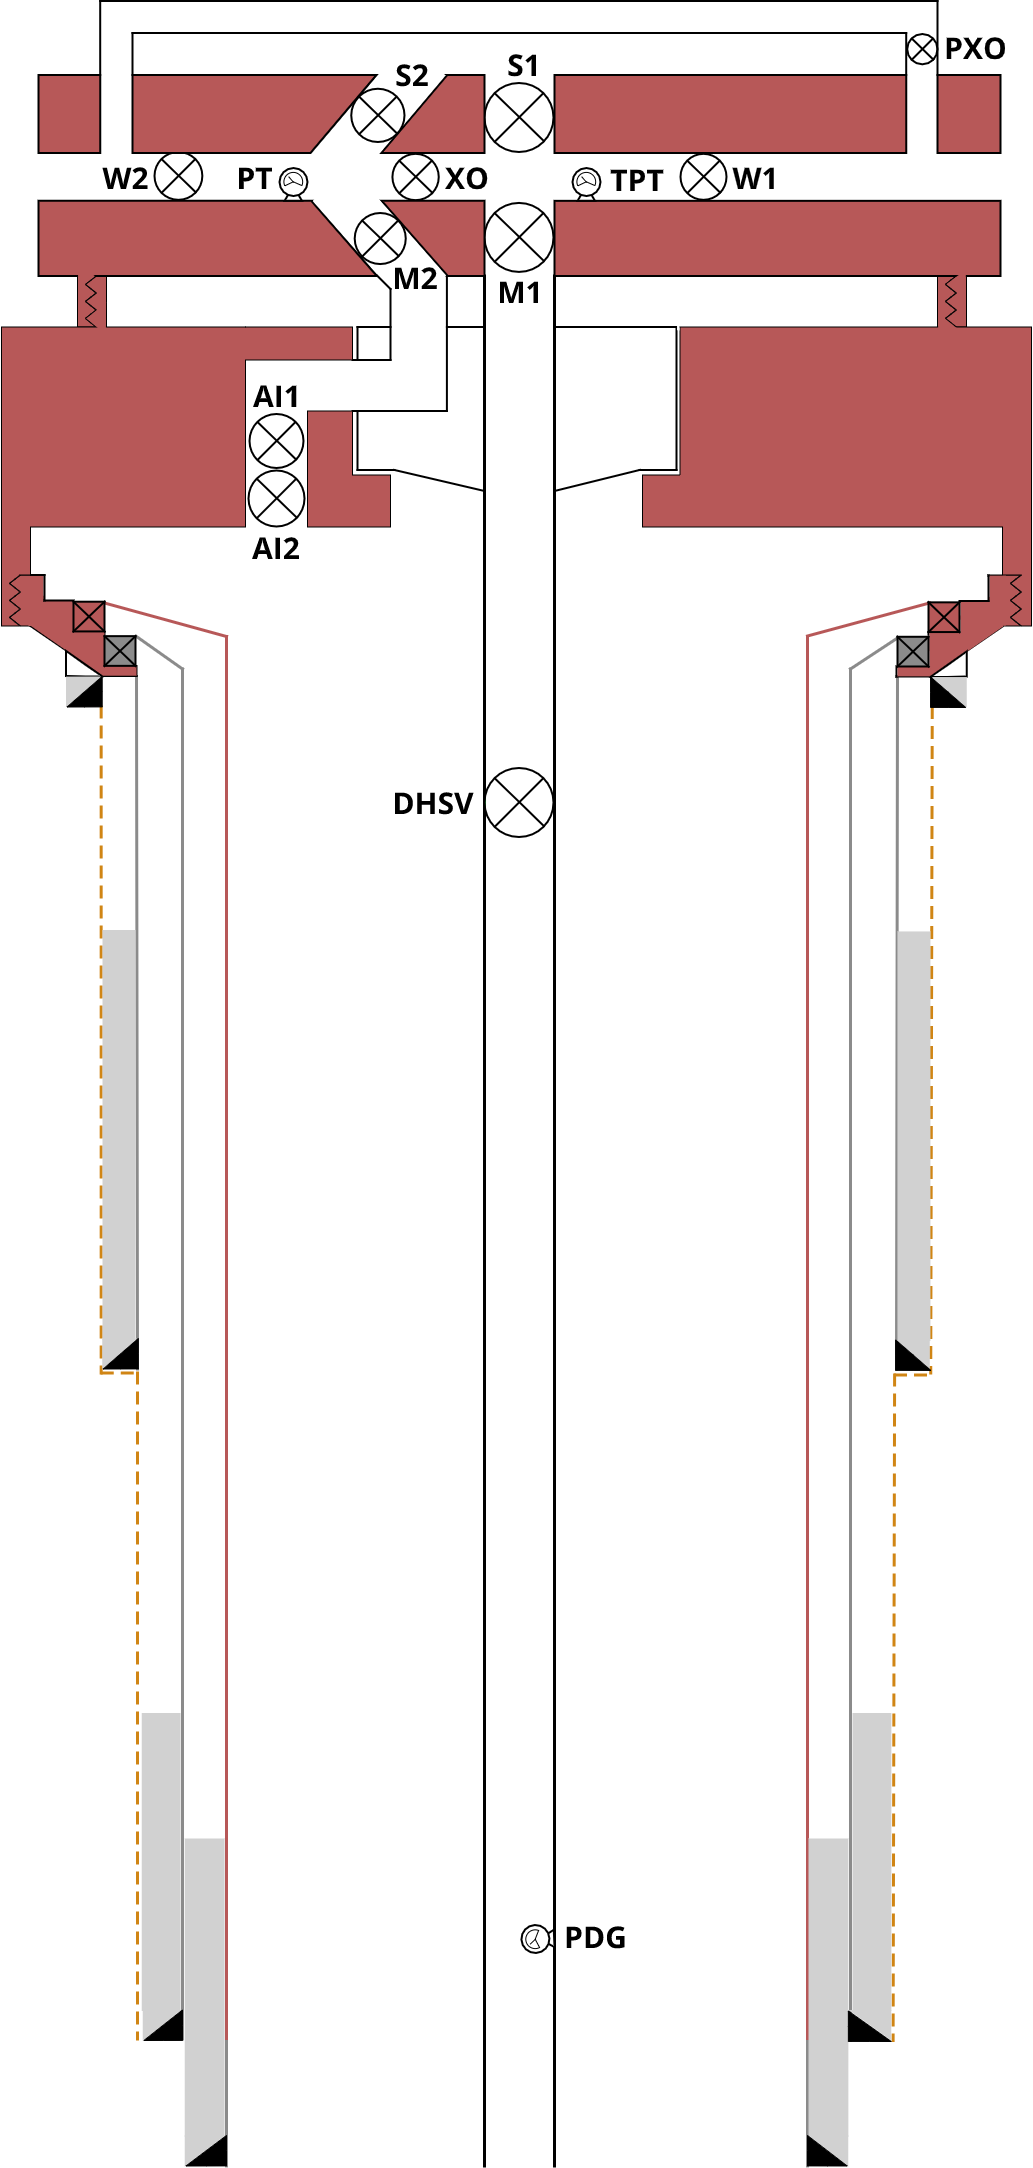
\includegraphics[width=0.42\textwidth]{esquema_vazio.png}
\caption{Disposição típica de válvulas e sensores em um poço submarino. Os medidores
PDG, TPT e PT ocupam posições fixas ao longo do caminho do fluido, e cada válvula ---
DHSV, M1, M2, W1, W2, XO, PXO e a reguladora --- define um estado operacional distinto.
Adaptado de \citet{aranha2023system}.}
\label{fig:dominio-esquema}
\end{figure}

A \cref{fig:dominio-esquema} situa os sensores no caminho do fluido. Essa geometria
explica boa parte do que vem a seguir: o PDG está a montante de tudo e responde primeiro
a variações no reservatório; o TPT está no leito marinho, onde o resfriamento é máximo;
o PT está a jusante da reguladora, e portanto enxerga a pressão já estrangulada. Duas
anomalias de mesma origem física produzem assinaturas diferentes em cada um desses
pontos, e é essa diferença que os modelos exploram.

\subsection{Os quatro sinais fundamentais}

\begin{description}[leftmargin=0pt,style=nextline,itemsep=0.5em]

\item[P-PDG --- pressão no medidor permanente de fundo.]
O \termo{medidor permanente de fundo}{permanent downhole gauge} (PDG) é instalado na
coluna de produção, próximo à zona produtora. Mede a pressão no ponto mais próximo do
reservatório que a instrumentação alcança. É o sinal mais informativo sobre o
comportamento do reservatório e sobre eventos de fundo, e é também o mais sujeito a
falha --- sua substituição exige intervenção com sonda.

\item[T-PDG --- temperatura no medidor permanente de fundo.]
Mede a temperatura do fluido no fundo. Varia lentamente em condições normais e reage a
mudanças de vazão com constante de tempo apreciável, o que a torna útil para
discriminar transitórios rápidos de mudanças de regime.

\item[P-TPT --- pressão no transdutor de temperatura e pressão.]
O \termo{transdutor de temperatura e pressão}{temperature and pressure transducer}
(TPT) está instalado na árvore de natal, a jusante do poço e a montante da válvula
reguladora. Mede a pressão na cabeça do poço.

\item[T-TPT --- temperatura no transdutor de temperatura e pressão.]
Temperatura na cabeça do poço. É a variável mais diretamente ligada à formação de
hidratos, já que a região da ANM é onde a combinação de baixa temperatura ambiente e
alta pressão é mais severa.

\end{description}

O conjunto 3W disponibiliza outras variáveis --- pressão a jusante da \ing{choke}
(P-JUS-CKP), temperatura a jusante, vazões de gás de elevação, posição da \ing{choke}.
Contudo, a maior parte dos trabalhos discutidos neste livro utiliza o subconjunto
\{P-PDG, T-PDG, P-TPT, T-TPT\}, por três razões: são as variáveis presentes em
praticamente todas as instâncias, são as menos afetadas por convenções de instalação
específicas de cada poço, e carregam a informação física essencial dos eventos de
interesse.

\begin{exemplo}{O gradiente entre fundo e cabeça}
A diferença $P_{\text{PDG}} - P_{\text{TPT}}$ é, aproximadamente, a perda de carga ao
longo da coluna de produção --- soma da componente hidrostática com a componente
friccional. Quando o fluido fica mais denso (aumento de BSW, por exemplo), a
componente hidrostática cresce e o gradiente aumenta. Quando a vazão cai, a componente
friccional diminui e o gradiente diminui.

Um único par de sensores permite, portanto, inferir mudanças em duas propriedades
distintas do escoamento. É por essa razão que o agente de linguagem do
\cref{cap:agente} calcula explicitamente um descritor de \emph{relação entre P-PDG e
P-TPT} --- ``mesma direção'', ``divergentes'' ou ``um estável'' --- e o entrega ao
modelo como evidência. A informação está na relação, não em cada sinal isolado.
\end{exemplo}

\subsection{Por que os sensores mentem}

Três patologias de instrumentação atravessam todo o livro e precisam ser enunciadas
desde já.

\begin{itemize}[leftmargin=*,itemsep=0.4em]
  \item \textbf{Congelamento.} O sensor para de atualizar e repete indefinidamente a
        última leitura válida. Uma série congelada tem desvio-padrão nulo e é
        trivialmente detectável --- desde que alguém procure por isso.
  \item \textbf{Perda de telemetria.} O valor se torna ausente ou é substituído por
        zero. Essa patologia terá importância inesperada no
        \cref{cap:resultados-agente}: em várias classes do 3W, o início da anomalia
        coincide com a perda dos medidores de fundo, o que cria uma correlação espúria
        entre ``anomalia'' e ``ausência de dado''.
  \item \textbf{Deriva.} O sensor mantém a dinâmica, mas seu nível absoluto se desloca
        lentamente. É a mais perigosa das três, porque não produz nenhuma assinatura
        óbvia e corrompe silenciosamente qualquer modelo calibrado em valores
        absolutos.
\end{itemize}

\begin{destaque}[Consequência de projeto]
As três patologias acima são o argumento técnico para trabalhar com \emph{variações
relativas a uma linha de base} em vez de valores absolutos. Essa decisão aparece de
formas diferentes ao longo do livro: normalização por janela no \cref{cap:dual},
padronização por poço no \cref{cap:segmentacao} e, de forma mais explícita, no cálculo
do descritor $\delta = \bar{e} - \bar{b}$ do \cref{cap:agente}.
\end{destaque}

\section{A taxonomia dos eventos indesejáveis}
\label{sec:dominio-taxonomia}

O conjunto 3W organiza os eventos em uma classe normal e nove classes de anomalia
\citep{VARGAS2019,VazVargas2026_3w2}. Descrevemos cada uma pelo mecanismo físico e pela
assinatura esperada.

\subsection{Classe 0 --- Estado normal}

Operação estável. Os sinais apresentam variação de baixa amplitude em torno de níveis
determinados pelo ponto de operação. É a classe de referência contra a qual todas as
demais são contrastadas e, em quantidade de amostras, a mais numerosa por larga
margem.

\subsection{Classe 1 --- Aumento abrupto de BSW}

\textbf{Mecanismo.} O \termo{teor de água e sedimentos}{basic sediment and water} (BSW)
é a fração volumétrica de água no fluido produzido. Um aumento abrupto indica avanço
da frente de água do aquífero ou de um poço injetor, ou ainda comunicação com uma zona
aquífera por falha de isolamento.

\textbf{Assinatura.} Água é mais densa que óleo. O aumento da fração de água eleva a
massa específica média da coluna, aumentando a pressão hidrostática. Espera-se aumento
de P-PDG e mudança no gradiente entre fundo e cabeça. A temperatura pode cair, já que a
água tem capacidade calorífica maior.

\textbf{Dificuldade.} O evento é gradual em muitos casos reais, o que o confunde com
declínio natural. A classe 1 apresenta desempenho apenas mediano em quase todos os
experimentos deste livro.

\subsection{Classe 2 --- Fechamento espúrio da DHSV}

\textbf{Mecanismo.} Perda de pressão na linha de controle hidráulico leva a DHSV a
fechar sem comando. O poço é isolado abaixo da válvula.

\textbf{Assinatura.} A mais nítida de todas. A pressão a montante da válvula (P-PDG)
sobe rapidamente, pois o reservatório continua a alimentar um volume fechado; a pressão
a jusante (P-TPT) despenca. As duas pressões divergem de forma inequívoca. As
temperaturas caem, pois cessa o transporte convectivo de calor do fundo.

\textbf{Consequência para os métodos.} A classe 2 é aquela em que praticamente todo
método deste livro atinge desempenho excelente --- 95\,\% no ensemble binário do
\cref{cap:closedworld}, 100\,\% na detecção de novidade do \cref{cap:resultados-agente}.
É o caso fácil, e serve de controle positivo: um método que falhe na classe 2 tem um
defeito estrutural.

\subsection{Classe 3 --- Golfadas severas}

\textbf{Mecanismo.} Em escoamento multifásico ascendente com \ing{riser} em catenária,
o líquido pode acumular-se no ponto baixo até bloquear a passagem de gás. A pressão a
montante cresce até vencer a coluna de líquido, que é então expelida em golfada. O
ciclo se repete com período de minutos a dezenas de minutos.

\textbf{Assinatura.} Oscilação periódica de grande amplitude em P-TPT e, com menor
amplitude, em P-PDG. É a única classe cuja assinatura característica é \emph{de
frequência}, não de nível.

\textbf{Consequência para os métodos.} Métodos que resumem uma janela por média e
desvio-padrão perdem a informação de periodicidade. Esse é um dos motivos pelos quais
o agente de linguagem do \cref{cap:agente} calcula uma \emph{razão de oscilação}
explícita, e um dos motivos pelos quais o desempenho da classe 3 melhora
substancialmente quando se usa segmentação temporal (\cref{cap:segmentacao}) em vez de
classificação de janela agregada.

\subsection{Classe 4 --- Instabilidade de fluxo}

\textbf{Mecanismo.} Regime de escoamento não estacionário sem a periodicidade regular
da golfada severa. Pode originar-se de instabilidade de gás de elevação, de
acoplamento entre reservatório e coluna, ou de operação próxima ao limite de
estabilidade.

\textbf{Assinatura.} Variabilidade aumentada em todos os sinais, sem padrão dominante.

\textbf{Advertência.} A classe 4 é \emph{sintomática}, não causal. Instabilidade de
fluxo é aquilo que se observa; o que a causou pode ser qualquer coisa. Essa
característica explica por que ela apresenta o pior desempenho médio do livro --- 69\,\%
no ensemble binário (\cref{cap:closedworld}), 18,5\,\% na primeira escolha do agente
(\cref{cap:resultados-agente}) --- e por que foi deliberadamente excluída de dois dos
três estudos com modelos de linguagem.

\subsection{Classe 5 --- Perda rápida de produtividade}

\textbf{Mecanismo.} Queda súbita do índice de produtividade do poço, por dano à
formação, colapso de canhoneado, produção de finos ou bloqueio na região próxima ao
poço.

\textbf{Assinatura.} Queda de vazão com aumento da pressão de fundo (o reservatório
deixa de conseguir entregar fluido à mesma taxa).

\textbf{Advertência.} Como a classe 4, é sintomática. O \cref{cap:mahalanobis} reporta
para ela o pior resultado de detecção de novidade de toda a Tabela correspondente:
67,5\,\% no espaço latente, contra mais de 96\,\% para as demais classes.

\subsection{Classe 6 --- Restrição rápida no PCK}

\textbf{Mecanismo.} Obstrução súbita da válvula reguladora de produção, por detrito,
falha mecânica ou deposição abrupta.

\textbf{Assinatura.} Aumento da pressão a montante da \ing{choke} (P-TPT) com queda da
pressão a jusante. Contraste com a classe 2: ali a divergência ocorre \emph{através da
DHSV}, no fundo; aqui, \emph{através da choke}, na superfície.

\subsection{Classe 7 --- Incrustação no PCK}

\textbf{Mecanismo.} Deposição gradual de sais inorgânicos --- carbonato de cálcio,
sulfato de bário --- na passagem da válvula reguladora, reduzindo progressivamente a
área efetiva.

\textbf{Assinatura.} Mesma direção da classe 6, mas em escala de tempo de semanas a
meses. A distinção entre 6 e 7 é, essencialmente, \emph{uma distinção de derivada}.

\subsection{Classe 8 --- Hidrato na linha de produção}

\textbf{Mecanismo.} Hidratos de gás natural são estruturas cristalinas em que moléculas
de água formam gaiolas que aprisionam moléculas de metano, etano e propano. Formam-se
em condições de alta pressão e baixa temperatura --- exatamente as condições de uma
linha de produção submarina em águas profundas. O tampão resultante obstrui o
escoamento.

\textbf{Assinatura.} Aumento da pressão a montante do tampão, queda a jusante, e queda
de temperatura. A dinâmica é de horas.

\textbf{Destaque.} A classe 8 é o objeto do experimento central do
\cref{cap:closedworld}, em que é comparada com um modelo termodinâmico analítico, e é
a classe escondida no experimento de conjunto aberto. No \cref{cap:mahalanobis}, ela
apresenta a razão de separação mais extrema já observada nos experimentos deste livro
--- 186,5 vezes no espaço latente.

\subsection{Classe 9 --- Hidrato na linha de serviço}

\textbf{Mecanismo.} O mesmo da classe 8, mas na linha de serviço (anular ou linha de
injeção de gás), que opera em condições distintas e é menos instrumentada.

\textbf{Assinatura.} Semelhante à classe 8, porém observada indiretamente, por reflexo
sobre a linha de produção.

\textbf{Advertência.} A classe 9 é a mais escassa em número de instâncias e a de pior
desempenho consistente. No \cref{cap:resultados-agente}, o agente acerta 7,1\,\% na
primeira tentativa e não converge para um nome consensual quando solicitado a batizar
o evento como novidade.

\section{Além do 3W: eventos de completação inteligente}
\label{sec:dominio-icv}

Dois eventos discutidos neste livro não pertencem ao conjunto 3W. Vêm de dados
proprietários e cumprem um papel metodológico específico: \emph{servem de novidade
genuína}, isto é, de classe que o sistema comprovadamente nunca viu.

\begin{description}[leftmargin=0pt,style=nextline,itemsep=0.5em]

\item[Falha de ICV.] A válvula de controle de intervalo não responde ao comando, ou
responde parcialmente, ou apresenta vazamento entre zonas. A assinatura é um degrau de
pressão e vazão que não corresponde a nenhum comando registrado. No
\cref{cap:mundoaberto}, instâncias de falha de ICV são apresentadas a um sistema
treinado apenas nas nove classes do 3W: 48\,\% são classificadas como pertencentes a
alguma classe conhecida e 52\,\% são corretamente marcadas como desconhecidas e
encaminhadas ao estágio de agrupamento.

\item[Operação de válvula.] Manobras programadas de abertura e fechamento. São
\emph{eventos normais} cuja assinatura se assemelha à de anomalias --- o caso clássico
do falso positivo legítimo. Um sistema que não distinga uma operação programada de um
fechamento espúrio é inútil em campo.

\end{description}

\begin{destaque}[Por que isso importa metodologicamente]
Avaliar detecção de novidade escondendo uma classe do próprio conjunto de treinamento é
válido, mas otimista: a classe escondida foi gerada pelo mesmo processo de coleta,
rotulada pela mesma equipe, com a mesma instrumentação. Uma classe genuinamente externa
--- vinda de outro conjunto de poços, com outra completação --- é um teste mais duro.
Os dois eventos acima cumprem esse papel.
\end{destaque}

\section{Uma taxonomia por assinatura}

Encerramos com uma reorganização das nove classes que será útil em todos os capítulos
seguintes. Em vez de agrupá-las por mecanismo, agrupamo-las por \emph{aquilo que o
algoritmo vê}.

\begin{center}
\small
\begin{tabular}{p{3.4cm} p{2.0cm} p{7.2cm}}
\toprule
\textbf{Assinatura} & \textbf{Classes} & \textbf{Implicação para o método} \\
\midrule
Divergência entre dois sinais de pressão & 2, 6 & Facilmente capturada por
descritores de relação entre sensores; alto desempenho universal. \\[0.3em]
Oscilação periódica & 3 & Exige preservação da estrutura temporal; penaliza
agregação por média. \\[0.3em]
Rampa lenta & 1, 7 & Exige janela longa; confunde-se com deriva de sensor e com
declínio natural. \\[0.3em]
Degrau com queda de temperatura & 8, 9 & Bem separável quando há dados de
temperatura confiáveis; a classe 9 sofre por escassez. \\[0.3em]
Aumento de variabilidade sem padrão & 4, 5 & Sintomática; baixa separabilidade
intrínseca. Candidata a tratamento diferenciado. \\
\bottomrule
\end{tabular}
\end{center}

Essa tabela antecipa a proposta de \emph{divisão de trabalho por classe} do
\cref{cap:sintese}: em vez de exigir que um único modelo trate igualmente as cinco
famílias de assinatura, atribui-se a cada família o componente que a trata melhor.

\resumocapitulo{%
Um poço submarino é observado por um punhado de sensores --- essencialmente pressão e
temperatura no fundo (PDG) e na cabeça (TPT) --- cujas leituras estão sujeitas a
congelamento, perda de telemetria e deriva. As nove classes de anomalia do conjunto 3W
diferem radicalmente em mecanismo físico, escala temporal e assinatura: há degraus
nítidos (fechamento espúrio de DHSV), oscilações periódicas (golfadas), rampas lentas
(incrustação) e classes meramente sintomáticas (instabilidade de fluxo, perda de
produtividade). Essa heterogeneidade é a razão estrutural pela qual nenhum modelo único
apresenta bom desempenho em todas as classes, e é o ponto de partida da arquitetura
modular defendida neste livro. Eventos de completação inteligente --- falha de ICV e
operação de válvula --- fornecem, por serem externos ao 3W, testes rigorosos de
detecção de novidade.}

\begin{exercicios}
\item Desenhe, à mão, as curvas esperadas de P-PDG e P-TPT ao longo de trinta minutos
      para: (a) fechamento espúrio da DHSV; (b) restrição rápida no PCK. Indique
      claramente em que ponto as duas assinaturas se distinguem e qual descritor
      numérico capturaria essa distinção.

\item A diferença $P_{\text{PDG}} - P_{\text{TPT}}$ combina componente hidrostática e
      componente friccional. Para cada uma das classes 1, 2, 5 e 8, diga se você espera
      que essa diferença aumente, diminua ou permaneça estável, e justifique fisicamente.

\item As classes 6 e 7 compartilham a mesma assinatura qualitativa e diferem apenas na
      escala de tempo. Proponha dois descritores numéricos que as separariam de forma
      robusta e discuta como o comprimento da janela de observação afeta cada um deles.

\item Argumente a favor e contra a seguinte proposta: ``as classes 4 e 5 deveriam ser
      removidas do catálogo de classificação e tratadas apenas como sinalizadores de
      atenção''. Considere as consequências para a métrica global, para o operador e
      para o registro histórico de eventos.

\item Um sensor de fundo apresenta deriva de $+2$\,bar por mês. Descreva o efeito
      dessa deriva sobre: (a) um detector de anomalia baseado em limiar absoluto;
      (b) um detector baseado em erro de reconstrução de autoencoder treinado há seis
      meses; (c) um descritor de variação relativa à linha de base imediatamente
      anterior ao evento. Ordene as três abordagens por robustez.

\item Consulte a documentação do conjunto 3W \citep{VazVargas2026_3w2} e liste todas as
      variáveis disponíveis. Para cada variável não utilizada neste livro, argumente se
      ela poderia ou não contribuir para separar as classes 4 e 5.
\end{exercicios}

\begin{leituras}
\item \citet{VARGAS2019} descrevem a origem operacional de cada classe do 3W. É a fonte
      primária para o conteúdo da \cref{sec:dominio-taxonomia}.
\item \citet{VazVargas2026_3w2} apresentam a versão 2.0 do conjunto, com classes
      adicionais e revisão da rotulação.
\item \citet{Safamirzaei2015} tratam da termodinâmica de formação de hidratos, base do
      modelo analítico usado no \cref{cap:closedworld}.
\item \citet{aranha2023system} e \citet{Aranha2024} descrevem sistemas de monitoramento
      em operação, com ênfase nos requisitos práticos que raramente aparecem em
      artigos metodológicos.
\end{leituras}

\chapter{Os dados: séries temporais de poços e o conjunto 3W}
\label{cap:dados}

\begin{objetivos}
Ao final deste capítulo, você será capaz de:
\begin{itemize}[leftmargin=*,itemsep=0.2em]
  \item formalizar uma série temporal multivariada de poço e definir janela, passo e
        rótulo;
  \item descrever a estrutura do conjunto 3W nas versões 1.0 e 2.0, incluindo a
        distinção entre instâncias reais, simuladas e desenhadas à mão;
  \item explicar a rotulação em três estados --- normal, transiente e anômalo --- e
        distinguir rótulo por amostra de rótulo por instância;
  \item identificar as principais armadilhas do conjunto: desbalanceamento, valores
        ausentes, sensores congelados, vazamento temporal e correlação espúria entre
        anomalia e perda de telemetria;
  \item projetar um protocolo de particionamento que evite vazamento entre treino e
        teste.
\end{itemize}
\end{objetivos}

\section{Formalização}

\begin{definicao}{Série temporal multivariada de poço}
Uma série temporal multivariada de poço é uma função
$\vect{x} : \mathcal{T} \to \R^{S}$, onde $\mathcal{T} \subset \mathbb{Z}$ é um
conjunto de instantes amostrados a intervalo regular $\Delta t$ e $S$ é o número de
sensores. Escrevemos $\vect{x}_t = (x_t^{(1)}, \dots, x_t^{(S)})^{\top}$ para a leitura
conjunta no instante $t$, e $x_t^{(s)}$ para a leitura do sensor $s$.
\end{definicao}

No conjunto 3W, $\Delta t = \SI{1}{\second}$ e uma instância típica cobre de algumas
horas a alguns dias. O subconjunto de sensores usado ao longo deste livro é, salvo
menção em contrário, $S = 4$, com os canais P-PDG, T-PDG, P-TPT e T-TPT descritos na
\cref{sec:dominio-sensores}.

\begin{definicao}{Janela deslizante}
Dada uma série $\vect{x}$, um comprimento de janela $T$ e um passo $h$, a
\termo{janela deslizante}{sliding window} de índice $i$ é a matriz
\[
  \mat{X}_i = \big[\, \vect{x}_{t_0 + ih},\; \vect{x}_{t_0 + ih + 1},\;
  \dots,\; \vect{x}_{t_0 + ih + T - 1} \,\big]^{\top} \in \R^{T \times S}.
\]
Quando $h < T$ as janelas se sobrepõem; quando $h = T$ elas são disjuntas.
\end{definicao}

A janela é a unidade de entrada de praticamente todos os modelos deste livro, e sua
parametrização varia de forma significativa entre eles. A \cref{tab:dados-janelas}
consolida as escolhas, o que é útil como referência ao longo da leitura.

\begin{table}[htbp]
\centering
\caption{Parametrização de janela adotada em cada capítulo deste livro.}
\label{tab:dados-janelas}
\small
\begin{tabular}{llll}
\toprule
\textbf{Capítulo} & \textbf{$T$ (amostras)} & \textbf{$S$} & \textbf{Passo $h$} \\
\midrule
\cref{cap:dual}         & 500                & 5 & contínuo (tempo real) \\
\cref{cap:binarios,cap:closedworld} & 150 a 7500 (varrido) & 8 & sobreposto \\
\cref{cap:mundoaberto}  & 200                & 4 & sobreposto \\
\cref{cap:segmentacao,cap:mahalanobis} & 200 & 4 & 100 (\SI{5}{\second} de avanço) \\
\cref{cap:agente}       & segmento variável  & 4 & --- (segmentos rotulados) \\
\bottomrule
\end{tabular}
\end{table}

\begin{destaque}[A escolha de $T$ não é livre]
O comprimento da janela impõe um compromisso duplo. Janelas curtas permitem resposta
rápida, mas não contêm informação suficiente para eventos lentos --- uma janela de
\SI{150}{\second} não pode, em princípio, distinguir incrustação (classe 7) de
restrição rápida (classe 6). Janelas longas capturam eventos lentos, mas atrasam a
detecção e diluem transientes curtos na média. O \cref{cap:closedworld} quantifica
esse compromisso com uma varredura de catorze valores de $T$.
\end{destaque}

\section{O conjunto 3W}

\subsection{Origem e propósito}

O 3W --- o nome registra que o conjunto reúne instâncias de \emph{três} procedências
distintas (reais, simuladas e desenhadas à mão) de eventos indesejáveis que ocorrem em
poços (\ing{wells}) de petróleo \citep{Petrobras3W} --- foi publicado pela Petrobras
com o objetivo explícito de dar à comunidade acadêmica um banco de dados realista para
detecção e classificação de eventos \citep{VARGAS2019}. Antes dele, a literatura da
área trabalhava quase exclusivamente com dados simulados ou proprietários, o que
tornava impossível comparar métodos.

\subsection{Versão 1.0}

A versão original contém \num{1984} instâncias distribuídas entre a classe normal e
oito classes de anomalia. Cada instância é um arquivo CSV com uma coluna de tempo,
colunas de sensores e uma coluna de rótulo por amostra.

\subsection{Versão 2.0}

A versão 2.0 \citep{VazVargas2026_3w2} amplia o conjunto para \num{2228} instâncias e
\num{10} classes (normal mais nove anomalias), revisa a rotulação de instâncias da
versão anterior e acrescenta metadados de poço. Os trabalhos discutidos nos
\cref{cap:dual,cap:binarios,cap:mundoaberto} foram desenvolvidos sobre a versão 1.0; os
dos \cref{cap:segmentacao,cap:mahalanobis,cap:agente} incorporam a versão 2.0.

\begin{destaque}[Comparabilidade entre versões]
Números de acurácia obtidos em versões diferentes do 3W \emph{não são diretamente
comparáveis}. A revisão de rótulos da versão 2.0 alterou a fronteira entre normal e
transiente em várias instâncias, e a inclusão de novas instâncias mudou a distribuição
de classes. Sempre que este livro compara resultados de capítulos distintos, a versão
utilizada é declarada.
\end{destaque}

\subsection{Três procedências}

Cada instância do 3W pertence a uma de três procedências, identificada pelo prefixo do
nome do arquivo:

\begin{description}[leftmargin=0pt,style=nextline,itemsep=0.5em]

\item[Real (\texttt{WELL-\dots}).] Registro efetivo de um poço em operação, com todos
os defeitos que isso implica: ruído, lacunas, deriva, comportamento idiossincrático.
É a única procedência que sustenta conclusões sobre desempenho em campo.

\item[Simulado (\texttt{SIMULATED-\dots}).] Gerado por simulador de escoamento
multifásico. Tem a vantagem de cobrir condições raras e a desvantagem de refletir as
hipóteses do simulador. Útil para aumentar a amostra de classes escassas.

\item[Desenhado à mão (\texttt{DRAWN-\dots}).] Construído manualmente por especialistas
para ilustrar a assinatura canônica de um evento. \emph{Não deve ser usado para
avaliação}: são exemplos idealizados, e um modelo avaliado sobre eles reporta um
desempenho que não se sustenta em campo.

\end{description}

\begin{destaque}[Uma decisão de projeto recorrente]
O trabalho descrito no \cref{cap:agente} adota a seguinte política, que recomendamos:
usar exclusivamente instâncias reais; recorrer a simuladas apenas quando a classe tem
menos de trinta instâncias reais; e excluir integralmente as desenhadas à mão. Essa
política reduz o tamanho do conjunto e piora os números publicados --- e é exatamente
por isso que ela é correta.
\end{destaque}

\section{A rotulação}

\subsection{Três estados por amostra}

O 3W rotula \emph{cada amostra} de cada instância com um de três estados:

\begin{center}
\small
\begin{tabular}{cll}
\toprule
\textbf{Código} & \textbf{Estado} & \textbf{Significado} \\
\midrule
$0$        & Normal    & Operação estável, anterior ao evento. \\
$100 + k$  & Transiente& Transição em curso para a anomalia de classe $k$. \\
$k$        & Anômalo   & Regime anômalo estabelecido da classe $k$. \\
\bottomrule
\end{tabular}
\end{center}

O estado transiente é a contribuição mais original --- e mais problemática --- do
esquema de rotulação. Ele reconhece que a passagem de normal para anômalo não é
instantânea, e que existe um intervalo em que o evento já começou mas ainda não se
manifestou plenamente. Do ponto de vista operacional, \emph{o transiente é exatamente
onde a detecção tem valor}: detectar depois que o regime anômalo se estabeleceu é tarde
demais.

\begin{destaque}[O que fazer com o transiente]
Três políticas convivem na literatura e neste livro:
\begin{enumerate}[leftmargin=*,itemsep=0.2em]
  \item \textbf{Descartar} as amostras transientes do treinamento. Produz classes mais
        puras e números melhores, ao custo de tornar o modelo cego justamente à fase
        que interessa.
  \item \textbf{Tratar como anômalo}. Favorece detecção precoce e aumenta o falso
        positivo.
  \item \textbf{Tratar como classe própria}. Triplica o número de classes e agrava o
        desbalanceamento.
\end{enumerate}
Os trabalhos deste livro adotam predominantemente a segunda política. A métrica SoftED
do \cref{cap:segmentacao} foi introduzida precisamente para avaliar a detecção com
tolerância temporal, tornando a questão menos binária.
\end{destaque}

\subsection{Rótulo por instância}

Além do rótulo por amostra, cada instância possui um rótulo global --- a classe do
evento que ela contém. Essa distinção gera duas famílias de métricas que \emph{não
podem ser confundidas}:

\begin{itemize}[leftmargin=*,itemsep=0.3em]
  \item \textbf{Métrica por amostra}: fração de amostras corretamente rotuladas.
        Dominada pelas instâncias mais longas e pela classe normal.
  \item \textbf{Métrica por instância}: fração de instâncias em que o evento foi
        corretamente identificado. É a que corresponde à pergunta operacional.
\end{itemize}

\begin{exemplo}{A diferença em números}
No \cref{cap:mundoaberto}, o classificador binário da classe 6 apresenta acurácia média
por amostra de $0{,}75 \pm 0{,}13$ e acurácia média por instância de
$0{,}34 \pm 0{,}42$. O desvio-padrão enorme na segunda métrica revela o que a primeira
esconde: o modelo acerta quase todas as amostras de algumas instâncias e erra quase
todas as de outras. Uma média de $0{,}75$ por amostra é compatível com ``funciona bem
em metade dos poços e não funciona na outra metade''.
\end{exemplo}

\section{As armadilhas}

\subsection{O estado das válvulas muda a estrutura de correlação}

Antes das armadilhas de rotulação, uma armadilha de estacionariedade. As variáveis
observadas não guardam entre si uma relação fixa: a estrutura de correlação depende da
configuração das válvulas no momento da medição.

\begin{figure}[htbp]
\centering
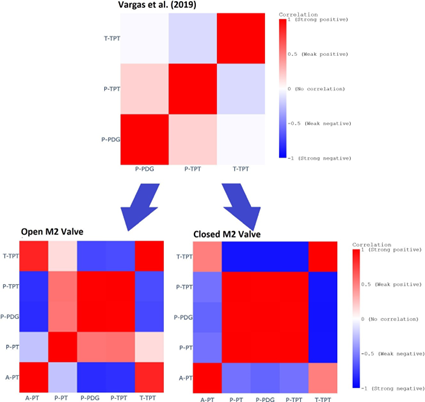
\includegraphics[width=0.62\textwidth]{correlation.png}
\caption{Matrizes de correlação entre os sinais de pressão e temperatura (PT, TPT e PDG),
calculadas separadamente para dados do 3W e para dados de operação com a válvula M2
aberta e fechada. Vermelho indica correlação positiva; azul, negativa. Adaptado de
\citet{aranha2023system}.}
\label{fig:dados-correlacao}
\end{figure}

A \cref{fig:dados-correlacao} mostra o efeito. Pares de sensores que se correlacionam
positivamente com a M2 aberta podem correlacionar-se de forma fraca ou invertida com a
M2 fechada, porque o caminho do fluido mudou. Um modelo treinado sobre a mistura dos dois
regimes aprende uma correlação média que não descreve nenhum dos dois.

\begin{destaque}[A consequência prática]
É por isso que o sistema do \cref{cap:dual} suspende a análise durante manobras de
válvula e retoma apenas após a estabilização, e é por isso que ele mantém modelos
distintos por configuração. Não é excesso de zelo: sem essa segmentação, toda manobra
programada vira um alarme.

O mesmo cuidado não é possível no 3W, que não distribui o estado das válvulas. Essa
ausência é uma limitação do conjunto, e não do método.
\end{destaque}

\subsection{Desbalanceamento}

A classe normal domina o conjunto por ordens de magnitude ao nível de amostra, e as
classes de anomalia são desbalanceadas entre si --- a classe 9 tem uma pequena fração
das instâncias da classe 7. As consequências são conhecidas e as contramedidas também:
métricas balanceadas (\cref{cap:aprendizado}), amostragem estratificada, ponderação de
classe na função de perda e, no caso do ensemble binário do \cref{cap:binarios},
subamostragem da classe negativa.

\subsection{Valores ausentes e sensores congelados}

Instâncias reais contêm lacunas. As estratégias usadas neste livro são:

\begin{itemize}[leftmargin=*,itemsep=0.3em]
  \item preenchimento com o último valor válido (\ing{forward fill}), adequado quando a
        lacuna é curta;
  \item preenchimento com o próximo valor válido (\ing{backward fill}), para lacunas no
        início da série;
  \item preenchimento pela média da janela, usado no \cref{cap:segmentacao};
  \item descarte da instância, quando a fração ausente excede um limiar.
\end{itemize}

Um sensor congelado não gera valor ausente --- gera um valor constante, que passa por
todos os filtros de qualidade baseados em nulos. Detectá-lo exige verificar
explicitamente $\std(x^{(s)}_{t:t+T}) < \epsilon$.

\subsection{A correlação espúria mais perigosa do 3W}
\label{sec:dados-telemetria}

Este é o achado mais desconfortável reportado neste livro, e ele aparece no
\cref{cap:resultados-agente}. Em várias classes do 3W --- notadamente 2, 6, 7 e 8 ---
o instante de início da anomalia coincide, com frequência muito acima do acaso, com a
perda dos medidores de fundo: P-PDG e T-PDG tornam-se ausentes ou zerados.

A explicação provável é banal e não tem nada a ver com física de poços. Muitos eventos
indesejáveis são acompanhados de intervenção, e intervenção frequentemente implica
reconfiguração da aquisição. O rótulo de anomalia e a interrupção da telemetria têm uma
causa comum.

\begin{destaque}[Por que isso importa]
Um modelo treinado nesses dados pode aprender ``se os sensores de fundo sumiram, é
anomalia''. Essa regra tem alto desempenho no conjunto de teste e valor operacional
próximo de zero. Pior: ela é invisível às métricas usuais.

Foi um modelo de linguagem, ao ser solicitado a \emph{descrever em texto} o que
observava, que tornou o padrão explícito: em quatro das sete classes analisadas, a
descrição gerada continha a expressão ``perda de telemetria de fundo''. O episódio é o
argumento mais forte deste livro a favor da explicabilidade --- não porque o modelo de
linguagem classifique melhor, mas porque ele \emph{fala}, e ao falar expõe o que o
classificador silencioso teria escondido.
\end{destaque}

\subsection{Vazamento temporal e vazamento entre poços}

Duas formas de vazamento comprometem avaliações neste domínio.

\begin{description}[leftmargin=0pt,style=nextline,itemsep=0.4em]

\item[Vazamento temporal.] Ocorre quando janelas sobrepostas de uma mesma instância
são distribuídas entre treino e teste. Como janelas adjacentes compartilham a maior
parte de suas amostras, o modelo essencialmente memoriza. A contramedida é a
\emph{divisão temporal}: os primeiros 80\,\% de cada instância para treino, os últimos
20\,\% para teste, sem sobreposição na fronteira. É o protocolo adotado no
\cref{cap:closedworld}.

\item[Vazamento entre poços.] Ocorre quando janelas de um mesmo poço aparecem em treino
e teste. O modelo aprende as idiossincrasias daquele poço --- nível de pressão
característico, ruído do sensor --- em vez da assinatura do evento. A contramedida é a
\emph{divisão por poço}, mais rigorosa e mais realista. O \cref{cap:segmentacao} reporta
resultados por poço individual justamente para expor a variabilidade que uma média
global esconde.

\end{description}

\begin{exemplo}{Quanto custa fazer certo}
No \cref{cap:segmentacao}, o desempenho da U-Net varia de $0{,}720$ de acurácia no poço
F1 a $0{,}975$ no poço C2. A média global, $0{,}863 \pm 0{,}082$, só é informativa
porque vem acompanhada do desvio-padrão e da tabela completa. Uma avaliação com
divisão aleatória de janelas reportaria um número maior e menos honesto.
\end{exemplo}

\section{Pré-processamento}

As etapas de pré-processamento empregadas no livro formam um repertório pequeno.

\begin{enumerate}[leftmargin=*,itemsep=0.45em]

\item \textbf{Tratamento de ausentes}, conforme descrito acima.

\item \textbf{Normalização Min-Max} para o intervalo $[0,1]$:
\[
  \tilde{x} = \frac{x - \min(x)}{\max(x) - \min(x)}.
\]
Usada no \cref{cap:dual}, onde o autoencoder tem saída sigmoide. Sensível a
\ing{outliers} e ao intervalo de calibração.

\item \textbf{Padronização} (escore $z$):
\[
  \tilde{x} = \frac{x - \mu}{\sigma}.
\]
Usada nos \cref{cap:segmentacao,cap:mahalanobis}. Preferível quando o modelo assume
distribuição aproximadamente gaussiana --- caso, notadamente, da distância de
Mahalanobis.

\item \textbf{Filtragem por transformada \ing{wavelet}.} Decomposição com \ing{wavelet}
de Daubechies db4 em três níveis, aplicação de limiar suave aos coeficientes de detalhe
e reconstrução. Remove ruído de alta frequência preservando descontinuidades --- o que
um filtro passa-baixas convencional não faz. É particularmente relevante aqui, já que
as assinaturas de interesse \emph{são} descontinuidades.

\item \textbf{Injeção de ruído} de 0 a 0,5\,\% durante o treinamento, empregada no
\cref{cap:dual} como regularização e para tornar o autoencoder robusto à variabilidade
de instrumentação entre poços.

\end{enumerate}

\begin{destaque}[O conjunto de ajuste importa]
Aplicar padronização e, em seguida, normalização Min-Max não produz dois efeitos
distintos quando ambas são ajustadas sobre as mesmas amostras. Nesse caso, a
transformação afim da primeira etapa é cancelada pela segunda e o resultado coincide
com a normalização Min-Max direta. A composição só acrescenta informação quando os
parâmetros são estimados sobre referências diferentes --- por exemplo, média e desvio
do regime de base de cada poço, seguidos de limites globais estimados exclusivamente no
conjunto de treinamento. Por isso, uma implementação reprodutível deve registrar não
apenas a ordem, mas também os dados usados para ajustar cada transformação.
\end{destaque}

\begin{destaque}[Prática]
Todo o percurso deste capítulo --- carga dos arquivos do 3W, comparação entre os quatro
métodos de escalonamento, janelamento e partição por validação cruzada --- está
implementado e executável no recurso descrito no \cref{cap:pratica}, no caderno
\texttt{1\_data\_treatment} \citep{Lopes2026Intro3W}.
\end{destaque}

\resumocapitulo{%
O conjunto 3W é a referência pública da área, com \num{1984} instâncias e oito classes
de anomalia na versão 1.0 e \num{2228} instâncias e nove classes na versão 2.0. Suas
instâncias têm três procedências --- real, simulada e desenhada à mão --- e apenas as
reais sustentam conclusões operacionais. A rotulação por amostra em três estados
(normal, transiente, anômalo) reconhece que eventos têm início gradual, e o tratamento
dado ao estado transiente é uma decisão de projeto com efeito direto sobre a detecção
precoce. As principais armadilhas são o desbalanceamento severo, os sensores congelados
que passam por filtros de nulos, o vazamento temporal e entre poços em protocolos de
avaliação descuidados e, sobretudo, a correlação espúria entre início de anomalia e
perda de telemetria de fundo --- um artefato de coleta capaz de produzir modelos com
alto desempenho e nenhum valor.}

\begin{exercicios}
\item Uma instância do 3W tem \num{86400} amostras (um dia a \SI{1}{\hertz}). Calcule
      quantas janelas de $T = 200$ com passo $h = 100$ ela produz. Em seguida, calcule a
      fração de amostras compartilhadas entre duas janelas consecutivas e discuta o
      impacto disso sobre uma divisão aleatória treino/teste.

\item Implemente um detector de sensor congelado: dado um sinal e uma janela, retorne
      as regiões em que o desvio-padrão fica abaixo de $\epsilon$. Aplique-o a
      instâncias reais do 3W e reporte a fração de amostras afetadas por classe.
      Discuta se essa fração é uniforme entre classes e o que uma não uniformidade
      implicaria.

\item Compare experimentalmente três políticas de tratamento do estado transiente
      (descartar, tratar como anômalo, classe própria) em um classificador binário
      simples para a classe 2. Reporte acurácia balanceada e a distância temporal média
      entre o início real do evento e a primeira detecção.

\item Considere o achado da \cref{sec:dados-telemetria}. Proponha um experimento
      controlado que quantifique a contribuição da perda de telemetria para o
      desempenho de um classificador. Dica: pense em uma ablação em que a informação de
      ``dado ausente'' é deliberadamente removida.

\item Justifique matematicamente por que a normalização Min-Max é sensível a
      \ing{outliers} e a padronização é sensível à hipótese de simetria. Para cada uma,
      construa um exemplo numérico de dez pontos em que ela falha.

\item Projete um protocolo de validação cruzada para o 3W que simultaneamente:
      (a) evite vazamento entre poços; (b) mantenha a estratificação por classe;
      (c) garanta que cada classe apareça em pelo menos três dobras. Discuta se as três
      condições são sempre simultaneamente satisfazíveis dado o desbalanceamento do
      conjunto.
\end{exercicios}

\begin{leituras}
\item \citet{VARGAS2019} --- artigo original do 3W, com a descrição do processo de
      rotulação.
\item \citet{VazVargas2026_3w2} --- versão 2.0, com discussão explícita das limitações da
      versão anterior.
\item \citet{marins2020fault} e \citet{Marins2021} --- primeiros trabalhos de referência
      sobre o 3W, úteis como linha de base e como ilustração das convenções de avaliação
      que se consolidaram na área.
\item \citet{carvalho2021flow} e \citet{bronstad2021data} --- perspectivas
      complementares sobre qualidade de dados em séries temporais industriais.
\end{leituras}

\chapter{Aprendizado de máquina e avaliação}
\label{cap:aprendizado}

\begin{objetivos}
Ao final deste capítulo, você será capaz de:
\begin{itemize}[leftmargin=*,itemsep=0.2em]
  \item formular detecção e classificação de anomalias como problemas de aprendizado
        supervisionado e não supervisionado;
  \item calcular e interpretar acurácia, acurácia balanceada, precisão, revocação,
        especificidade, medida $F_1$ e SMAPE;
  \item justificar por que a acurácia simples é enganosa em cenários desbalanceados e
        escolher a métrica adequada ao objetivo operacional;
  \item construir intervalos de confiança de Wilson para proporções e usá-los para
        decidir se uma diferença entre métodos é significativa;
  \item distinguir avaliação por amostra, por instância e por evento, e reconhecer
        quando cada uma responde à pergunta certa.
\end{itemize}
\end{objetivos}

\section{As duas formulações}

\subsection{Supervisionada}

Dispõe-se de pares $(\mat{X}_i, y_i)$ com $y_i \in \mathcal{K}$, e busca-se
$f_{\theta} : \R^{T \times S} \to \mathcal{K}$ que minimize o risco empírico
\[
  \hat{R}(\theta) = \frac{1}{n} \sum_{i=1}^{n} \mathcal{L}\big(f_{\theta}(\mat{X}_i), y_i\big).
\]
Para classificação binária, $\mathcal{L}$ é a entropia cruzada binária
\[
  \mathcal{L}(\hat{y}, y) = -\big[\, y \log \hat{y} + (1-y)\log(1-\hat{y}) \,\big],
\]
e para classificação multiclasse, a entropia cruzada categórica. Essa é a formulação do
ensemble binário (\cref{cap:binarios,cap:closedworld}) e da U-Net de segmentação
(\cref{cap:segmentacao}).

\subsection{Não supervisionada}

Dispõe-se apenas de $\mat{X}_i$. Duas subformulações interessam aqui:

\begin{itemize}[leftmargin=*,itemsep=0.35em]
  \item \textbf{Modelagem de normalidade.} Ajusta-se um modelo à classe normal e
        declara-se anômalo aquilo que se afasta dele. É o princípio do autoencoder com
        limiar de erro de reconstrução (\cref{cap:dual}) e da distância de Mahalanobis
        (\cref{cap:mahalanobis}).
  \item \textbf{Agrupamento.} Particiona-se um conjunto sem rótulos em grupos
        coerentes. É o mecanismo pelo qual instâncias rejeitadas como desconhecidas se
        tornam classes candidatas (\cref{cap:mundoaberto}).
\end{itemize}

\begin{destaque}[Uma terceira formulação, implícita]
Os \cref{cap:llm,cap:agente,cap:resultados-agente} usam um modelo de linguagem
\emph{sem qualquer treinamento sobre os dados de poço}. Não é aprendizado
supervisionado nem não supervisionado: é inferência com conhecimento prévio, guiada por
descritores numéricos. A avaliação, contudo, usa as mesmas métricas --- e é
precisamente por isso que este capítulo antecede aquela discussão.
\end{destaque}

\section{A matriz de confusão e o que se extrai dela}

Para um problema binário, com a convenção de que ``positivo'' significa ``anomalia
presente'':

\begin{center}
\small
\begin{tabular}{ll cc}
\toprule
& & \multicolumn{2}{c}{\textbf{Predito}} \\
\cmidrule(l){3-4}
& & Positivo & Negativo \\
\midrule
\multirow{2}{*}{\textbf{Real}}
& Positivo & VP & FN \\
& Negativo & FP & VN \\
\bottomrule
\end{tabular}
\end{center}

\begin{definicao}{Métricas fundamentais}
\begin{align}
\text{ACC} &= \frac{\text{VP} + \text{VN}}{\text{VP} + \text{VN} + \text{FP} + \text{FN}}
  \label{eq:acc}\\[0.4em]
\text{REC} &= \frac{\text{VP}}{\text{VP} + \text{FN}}
  \qquad \text{(revocação, \ing{recall}, sensibilidade)} \label{eq:rec}\\[0.4em]
\text{SP} &= \frac{\text{VN}}{\text{VN} + \text{FP}}
  \qquad \text{(especificidade)} \label{eq:sp}\\[0.4em]
\text{PR} &= \frac{\text{VP}}{\text{VP} + \text{FP}}
  \qquad \text{(precisão)} \label{eq:pr}\\[0.4em]
F_1 &= \frac{2 \cdot \text{PR} \cdot \text{REC}}{\text{PR} + \text{REC}}
  \label{eq:f1}
\end{align}
\end{definicao}

\begin{definicao}{Acurácia balanceada}
\begin{equation}
  \text{ACC}_b = \frac{\text{REC} + \text{SP}}{2}.
  \label{eq:accb}
\end{equation}
Equivale à média das acurácias por classe e, portanto, atribui o mesmo peso à classe
positiva e à negativa independentemente de sua frequência. Um classificador que sempre
prediz a classe majoritária tem $\text{ACC}_b = 0{,}5$, qualquer que seja o
desbalanceamento.
\end{definicao}

\begin{exemplo}{Por que a acurácia simples engana}
Considere um poço monitorado a \SI{1}{\hertz} durante trinta dias, com um único evento
de anomalia que dura duas horas. O número de amostras anômalas é
$2 \times 3600 = \num{7200}$; o de amostras normais, $30 \times 86400 - 7200 =
\num{2584800}$. A prevalência da anomalia é de aproximadamente $0{,}28\,\%$.

Um classificador que responda ``normal'' para toda amostra obtém
\[
  \text{ACC} = \frac{\num{2584800}}{\num{2592000}} \approx 0{,}9972,
\]
ou seja, $99{,}72\,\%$ de acurácia. Sua acurácia balanceada, contudo, é
$\text{ACC}_b = (0 + 1)/2 = 0{,}5$, sua revocação é zero e sua medida $F_1$ é
indefinida (ou zero, por convenção). O sistema é inútil e a acurácia simples não diz.
\end{exemplo}

\begin{destaque}[Qual métrica escolher]
A escolha deve seguir a consequência operacional do erro.
\begin{itemize}[leftmargin=*,itemsep=0.2em]
  \item Se o custo de \emph{perder} um evento domina (hidrato, integridade), priorize
        \textbf{revocação}.
  \item Se o custo de \emph{alarme falso} domina (fadiga de alarme, parada
        desnecessária), priorize \textbf{precisão}.
  \item Se ambos importam e não há razão para privilegiar um, use $F_1$.
  \item Se as classes são fortemente desbalanceadas e você quer uma leitura única,
        use $\text{ACC}_b$.
\end{itemize}
Este livro reporta, em geral, o conjunto completo, porque a escolha depende do leitor.
\end{destaque}

\section{Métricas de regressão e reconstrução}

Modelos que reconstroem um sinal, como os autoencoders dos
\cref{cap:dual,cap:mundoaberto,cap:mahalanobis}, precisam de uma medida de erro de
reconstrução. A escolha feita no \cref{cap:dual} é o SMAPE.

\begin{definicao}{Erro percentual absoluto médio simétrico}
\begin{equation}
  \text{SMAPE} = \frac{100\,\%}{n} \sum_{t=1}^{n}
  \frac{\left| \hat{x}_t - x_t \right|}
       {\big(\left| x_t \right| + \left| \hat{x}_t \right|\big)/2}.
  \label{eq:smape}
\end{equation}
\end{definicao}

O SMAPE tem três propriedades que o tornam adequado ao problema. É \emph{relativo},
logo comparável entre sensores de escalas diferentes --- pressão em bar e temperatura
em graus Celsius. É \emph{simétrico}, penalizando igualmente superestimação e
subestimação, ao contrário do erro percentual absoluto usual. E é \emph{limitado} a
$200\,\%$, o que impede que um único ponto próximo de zero domine a média, patologia
que compromete o erro percentual convencional.

\begin{destaque}[A armadilha do SMAPE]
O denominador anula-se quando $x_t = \hat{x}_t = 0$. Em séries normalizadas para
$[0,1]$, isso não é hipotético. A implementação deve adicionar um termo de
regularização $\epsilon$ ou tratar explicitamente o caso.
\end{destaque}

\section{Avaliação de detecção de eventos}

Há uma incompatibilidade estrutural entre as métricas apresentadas até aqui e a
pergunta operacional. As métricas por amostra tratam cada instante como um item
independente; a operação pergunta ``o evento foi detectado, e com que antecedência?''.

\begin{exemplo}{O problema do deslocamento}
Suponha que um evento comece no instante $t = \num{1000}$ e que um detector o sinalize
em $t = \num{1005}$. Do ponto de vista operacional, cinco segundos de atraso é uma
detecção essencialmente perfeita. Do ponto de vista de uma métrica por amostra, foram
cinco falsos negativos seguidos de acertos --- e se o detector tivesse sinalizado em
$t = \num{995}$, seriam cinco falsos positivos.

Uma métrica que penaliza igualmente ``cinco segundos adiantado'' e ``nunca detectou''
não está medindo o que interessa.
\end{exemplo}

A família SoftED \citep{Salles2024softed} resolve isso introduzindo uma tolerância
temporal $k$: uma detecção é creditada como verdadeiro positivo se ocorrer dentro de
$k$ amostras do evento real, com peso decrescente conforme a distância. O
\cref{cap:segmentacao} avalia a U-Net com $k = \num{1000}$ --- aproximadamente dezesseis
minutos --- e reporta separadamente a taxa de \emph{detecção precoce}, isto é, a fração
de eventos sinalizados antes do instante rotulado.

\begin{destaque}[Três níveis de avaliação]
Ao ler qualquer tabela deste livro, verifique primeiro o nível:
\begin{enumerate}[leftmargin=*,itemsep=0.15em]
  \item \textbf{Por amostra} --- cada instante conta. Domina o \cref{cap:dual} e o
        \cref{cap:segmentacao} (acurácia e IOU).
  \item \textbf{Por janela ou segmento} --- cada janela conta. Domina o
        \cref{cap:closedworld} e o \cref{cap:resultados-agente}.
  \item \textbf{Por evento} --- cada evento conta, com tolerância temporal. É o SoftED,
        no \cref{cap:segmentacao}.
\end{enumerate}
Números de níveis diferentes não são comparáveis, ainda que ambos se chamem
``acurácia''.
\end{destaque}

\subsection{A métrica de sobreposição para segmentação}

\begin{definicao}{Razão entre interseção e união}
Para uma região predita $\hat{A}$ e uma região real $A$, ambas subconjuntos do eixo
temporal,
\begin{equation}
  \text{IOU}(\hat{A}, A) = \frac{|\hat{A} \cap A|}{|\hat{A} \cup A|}.
  \label{eq:iou}
\end{equation}
\end{definicao}

O IOU é mais exigente que a acurácia por amostra porque não é inflado pela classe
majoritária: regiões corretamente identificadas como normais não entram no cálculo. É
por isso que, na tabela de segmentação do \cref{cap:segmentacao}, a acurácia global é
$94{,}00\,\%$ enquanto o IOU global é $85\,\%$.

\section{Métricas para \ing{ranking}: acurácia top-$k$}

Quando um sistema devolve uma lista ordenada de hipóteses em vez de uma única resposta,
a métrica natural é a acurácia top-$k$.

\begin{definicao}{Acurácia top-$k$}
Seja $R_i = (r_i^{(1)}, \dots, r_i^{(m)})$ a lista ordenada de classes candidatas
produzida para a instância $i$, e $y_i$ o rótulo verdadeiro. A acurácia top-$k$ é
\begin{equation}
  \text{ACC}@k = \frac{1}{n} \sum_{i=1}^{n}
  \mathbb{1}\!\left[\, y_i \in \{ r_i^{(1)}, \dots, r_i^{(k)} \} \,\right].
  \label{eq:topk}
\end{equation}
\end{definicao}

Essa métrica é central no \cref{cap:resultados-agente}, onde o agente de linguagem
devolve as três hipóteses mais prováveis com justificativa individual. A leitura
correta desses números exige contexto: para nove classes, um sistema aleatório obteria
$\text{ACC}@1 = 11{,}1\,\%$, $\text{ACC}@2 = 22{,}2\,\%$ e
$\text{ACC}@3 = 33{,}3\,\%$. Os valores observados --- $35{,}1\,\%$, $53{,}4\,\%$ e
$63{,}9\,\%$ --- são portanto cerca de três, duas e meia e duas vezes o acaso,
respectivamente.

\begin{destaque}[Top-$k$ não é uma métrica ``mais fácil'']
É comum descartar a acurácia top-3 como ``inflada''. Isso ignora o uso pretendido.
Quando o sistema é um \emph{assistente} que apresenta hipóteses a um especialista, a
pergunta certa é ``a resposta correta está entre as opções que ele considerou?''.
A acurácia top-1 é a métrica de um sistema autônomo; a top-$k$ é a métrica de um
sistema de apoio à decisão. O \cref{cap:agente} argumenta que a segunda é a arquitetura
apropriada para este domínio.
\end{destaque}

\section{Incerteza: intervalos de confiança para proporções}

Toda métrica reportada neste livro é uma estimativa a partir de amostra finita, e várias
delas vêm de amostras pequenas --- catorze instâncias na classe 9 do
\cref{cap:resultados-agente}, por exemplo. Reportar ``$7{,}1\,\%$'' sem intervalo é
irresponsável.

\begin{definicao}{Intervalo de Wilson}
Para $x$ sucessos em $n$ ensaios, com $\hat{p} = x/n$ e nível de confiança
correspondente a $z$ (com $z = 1{,}96$ para $95\,\%$), o intervalo de Wilson
\citep{Wilson1927} é
\begin{equation}
  \frac{\hat{p} + \dfrac{z^{2}}{2n} \;\pm\; z\sqrt{\dfrac{\hat{p}(1-\hat{p})}{n}
  + \dfrac{z^{2}}{4n^{2}}}}{1 + \dfrac{z^{2}}{n}}.
  \label{eq:wilson}
\end{equation}
\end{definicao}

O intervalo de Wilson é preferível ao intervalo normal (de Wald)
$\hat{p} \pm z\sqrt{\hat{p}(1-\hat{p})/n}$ por duas razões decisivas neste contexto:
ele nunca ultrapassa $[0,1]$, e continua bem definido quando $\hat{p} = 0$ ou
$\hat{p} = 1$ --- casos que ocorrem repetidamente nas tabelas por classe deste livro.

\begin{exemplo}{Uma diferença que não é diferença}
No \cref{cap:resultados-agente}, o agente atinge $\text{ACC}@1 = 35{,}1\,\%$ sobre
$n = 191$ segmentos, com intervalo de Wilson $[28{,}7\,\%;\ 42{,}1\,\%]$. Suponha que
um método alternativo obtenha $40{,}0\,\%$ sobre a mesma amostra. O intervalo do
segundo método seria aproximadamente $[33{,}3\,\%;\ 47{,}1\,\%]$, com sobreposição
substancial. Concluir que o segundo método é melhor seria injustificado.

O mesmo raciocínio aplicado às classes individuais é ainda mais severo: com $n = 15$,
o intervalo de Wilson para $\hat{p} = 0{,}267$ vai de aproximadamente $0{,}107$ a
$0{,}522$. Praticamente nenhuma comparação entre classes com essa amostra é
estatisticamente conclusiva --- o que não impede que os padrões qualitativos sejam
informativos.
\end{exemplo}

\begin{destaque}[Regra prática deste livro]
Toda proporção reportada com $n < 200$ vem acompanhada de intervalo de $95\,\%$. Toda
média sobre poços ou dobras vem acompanhada de desvio-padrão. Quando o desvio-padrão é
grande em relação à média --- como o $0{,}34 \pm 0{,}42$ do \cref{cap:mundoaberto} ---
o texto discute explicitamente o que isso significa.
\end{destaque}

\section{Validação}

\subsection{Validação cruzada estratificada}

Os \cref{cap:segmentacao,cap:mahalanobis} usam validação cruzada estratificada em cinco
dobras: o conjunto é particionado em cinco partes preservando a proporção de classes,
e cada parte serve uma vez como conjunto de teste. A estratificação é indispensável
sob desbalanceamento severo.

\subsection{Divisão temporal}

O \cref{cap:closedworld} usa divisão temporal $80/20$ dentro de cada instância, pelo
motivo exposto na \cref{cap:dados}: janelas sobrepostas distribuídas aleatoriamente
produzem vazamento.

\subsection{Avaliação por poço}

O protocolo mais rigoroso, adotado no \cref{cap:segmentacao}, avalia poço a poço e
reporta a tabela completa. Ele revela a variabilidade entre poços --- o desvio-padrão
de $0{,}187$ na acurácia do detector baseado em autoencoder --- que uma média
esconderia.

\begin{destaque}[Prática]
O caderno \texttt{4\_introduction\_to\_supervised\_learning}, descrito no
\cref{cap:pratica}, treina árvores, florestas, SVM e redes densas sobre o 3W e reporta as
métricas discutidas aqui \citep{Lopes2026Intro3W}. É o caminho mais curto para ver, em
dados reais, por que a acurácia simples engana sob desbalanceamento.
\end{destaque}

\resumocapitulo{%
A avaliação é a parte do método em que os erros são mais fáceis e mais caros. Sob o
desbalanceamento característico de dados de poço, a acurácia simples é sistematicamente
enganosa: um detector inútil atinge $99{,}7\,\%$. A acurácia balanceada, definida como a
média de revocação e especificidade, corrige o problema. A escolha entre precisão e
revocação deve seguir a consequência operacional do erro, não a conveniência do número.
Erros de reconstrução são medidos por SMAPE, relativo, simétrico e limitado. A avaliação
de detecção de eventos exige tolerância temporal, formalizada pela família SoftED, e a
avaliação de segmentação exige IOU além de acurácia. Sistemas que devolvem
\ing{rankings} são avaliados por acurácia top-$k$, que deve sempre ser lida contra a
linha de base do acaso. Toda proporção estimada de amostra pequena deve vir acompanhada
de intervalo de confiança de Wilson.}

\begin{exercicios}
\item Demonstre que, para um classificador que sempre prediz a classe majoritária,
      $\text{ACC}_b = 0{,}5$ independentemente da prevalência. Em seguida, mostre que
      $\text{ACC}_b$ é a média das acurácias condicionais a cada classe.

\item Um detector apresenta $\text{VP} = 45$, $\text{FN} = 15$, $\text{FP} = 90$ e
      $\text{VN} = \num{9850}$. Calcule ACC, $\text{ACC}_b$, PR, REC, SP e $F_1$.
      Comente a discrepância entre ACC e $F_1$ e diga qual você reportaria a um gerente
      de operação e por quê.

\item Mostre que o SMAPE é limitado superiormente por $200\,\%$. Construa em seguida uma
      série de dez pontos em que o erro percentual absoluto médio convencional diverge
      mas o SMAPE permanece finito.

\item Calcule o intervalo de Wilson de $95\,\%$ para $x = 1$ sucesso em $n = 14$ ensaios
      (o caso da classe 9 no \cref{cap:resultados-agente}). Compare com o intervalo de
      Wald e explique por que o segundo é inadequado.

\item Implemente a métrica SoftED com tolerância $k$ e aplique-a a um detector simples
      sobre uma instância do 3W. Trace a curva de $F_1$ em função de $k$ para
      $k \in \{10, 100, 500, 1000, 5000\}$ e discuta como escolher $k$ a partir de
      requisitos operacionais.

\item Um sistema devolve três hipóteses ordenadas para um problema de nove classes.
      Calcule a acurácia top-1, top-2 e top-3 esperadas sob escolha aleatória
      \emph{sem} repetição. Em seguida, calcule quantas vezes acima do acaso estão os
      valores $35{,}1\,\%$, $53{,}4\,\%$ e $63{,}9\,\%$ reportados no
      \cref{cap:resultados-agente}.

\item Discuta a seguinte proposta: ``para evitar a discussão sobre qual métrica usar,
      basta reportar todas''. Considere o problema de comparação múltipla e o risco de
      seleção da métrica mais favorável após ver os resultados.
\end{exercicios}

\begin{leituras}
\item \citet{Salles2024softed} introduzem a família SoftED e discutem em profundidade a
      inadequação das métricas por amostra para detecção de eventos.
\item \citet{Wilson1927} é o artigo original do intervalo que leva seu nome; curto e
      surpreendentemente legível.
\item \citet{Pimentel2014review} discutem, em sua revisão de detecção de novidade, os
      problemas específicos de avaliação quando a classe positiva é rara por
      construção.
\item \citet{Chollet2015} e \citet{scipy} documentam as implementações de referência das
      métricas discutidas aqui.
\end{leituras}

\chapter{Aprendizado profundo para séries temporais}
\label{cap:profundo}

\begin{objetivos}
Este capítulo é um panorama de referência, não um curso de aprendizado profundo: ele
apresenta apenas o que é necessário para acompanhar as arquiteturas usadas no restante
do livro. Ao final, você será capaz de:
\begin{itemize}[leftmargin=*,itemsep=0.2em]
  \item descrever a estrutura de um perceptron de múltiplas camadas e explicar por que
        ele é inadequado a séries temporais longas;
  \item explicar, no nível das equações de estado, o que as células LSTM e GRU fazem e
        que problema de gradiente elas atenuam;
  \item aplicar convoluções unidimensionais a sinais e calcular o campo receptivo de uma
        pilha convolucional;
  \item descrever a estrutura de um autoencoder, interpretar seu espaço latente e usar o
        erro de reconstrução como escore de anomalia;
  \item distinguir autoencoder, autoencoder variacional e rede de agrupamento profundo
        quanto ao que cada um otimiza;
  \item descrever a arquitetura U-Net e justificar por que suas conexões de atalho
        importam para segmentação;
  \item enunciar a equação da atenção e situar o Transformer no contexto deste livro ---
        nenhum modelo aqui treinado é um Transformer, e a arquitetura não é desenvolvida
        em detalhe.
\end{itemize}
\end{objetivos}

\section{Da regressão à rede profunda}

\subsection{O perceptron de múltiplas camadas}

Uma camada densa aplica uma transformação afim seguida de não linearidade:
\begin{equation}
  \vect{h}^{(\ell)} = \sigma\big( \mat{W}^{(\ell)} \vect{h}^{(\ell-1)} + \vect{b}^{(\ell)} \big),
  \label{eq:camada-densa}
\end{equation}
com $\vect{h}^{(0)} = \vect{x}$. Empilhando $L$ camadas obtém-se o \termo{perceptron de
múltiplas camadas}{multilayer perceptron} (MLP). As não linearidades usadas neste livro
são a ReLU, $\sigma(z) = \max(0, z)$, nas camadas ocultas, e a sigmoide,
$\sigma(z) = 1/(1 + e^{-z})$, nas saídas binárias.

Aplicar um MLP a uma série temporal exige achatá-la em um vetor de dimensão $T \cdot S$.
Para $T = 200$ e $S = 4$, isso resulta em \num{800} entradas --- exatamente a
representação ``bruta'' usada como linha de base no \cref{cap:mahalanobis}. O
procedimento funciona, mas descarta duas propriedades essenciais do sinal: a
\emph{ordem} (permutar os instantes produziria a mesma representação para uma rede sem
estrutura) e a \emph{invariância a translação} (o mesmo padrão em posição diferente
ativa pesos diferentes).

\begin{destaque}[Por que a linha de base bruta ainda aparece]
O \cref{cap:mahalanobis} reporta que classificadores binários sobre a representação
bruta de \num{800} dimensões atingem $0{,}691 \pm 0{,}162$ de acurácia, contra
$0{,}755 \pm 0{,}171$ sobre a representação latente de um classificador multiclasse. A
diferença é real, mas modesta --- e o fato de a representação bruta chegar tão perto é
informativo: as assinaturas dessas anomalias são, em boa medida, capturáveis por
estatísticas de primeira ordem.
\end{destaque}

\subsection{Regularização}

Três mecanismos são usados de forma recorrente:

\begin{itemize}[leftmargin=*,itemsep=0.3em]
  \item \textbf{\ing{Dropout}} \citep{srivastava14a}: durante o treinamento, cada
        unidade é zerada com probabilidade $p$. Nas arquiteturas deste livro, $p$ varia
        de $0{,}1$ a $0{,}5$, tipicamente decrescendo em direção à saída.
  \item \textbf{Normalização em lote} (\ing{batch normalization}): normaliza as ativações
        de cada camada pela média e variância do lote, acelerando a convergência e
        atuando como regularizador leve. Presente em todos os blocos da U-Net do
        \cref{cap:segmentacao}.
  \item \textbf{Parada antecipada} (\ing{early stopping}): interrompe o treinamento
        quando a perda de validação deixa de melhorar por um número fixo de épocas.
        O \cref{cap:closedworld} usa paciência de cinco épocas.
\end{itemize}

\section{Redes recorrentes}

\subsection{O problema}

Uma rede recorrente processa a sequência mantendo um estado oculto:
\begin{equation}
  \vect{h}_t = \sigma\big( \mat{W}_{hh}\vect{h}_{t-1} + \mat{W}_{xh}\vect{x}_t + \vect{b} \big).
  \label{eq:rnn}
\end{equation}
A retropropagação através do tempo desdobra essa recorrência em $T$ passos, e o
gradiente em relação a $\vect{h}_1$ envolve o produto de $T$ jacobianas. Se os autovalores
dominantes dessas matrizes forem menores que um, o gradiente decai exponencialmente e a
rede não aprende dependências longas; se forem maiores, ele explode. É o
\termo{problema do gradiente evanescente}{vanishing gradient problem}
\citep{SCHMIDHUBER201585}.

Para $T = 500$, como no \cref{cap:dual}, uma RNN simples é inviável.

\subsection{A célula LSTM}

A \termo{memória de curto prazo longa}{long short-term memory} (LSTM)
\citep{Hochreiter1997} introduz um estado de célula $\vect{c}_t$ que se propaga por
soma, não por produto matricial, e três portas que regulam o fluxo de informação:

\begin{align}
\vect{f}_t &= \sigma\big(\mat{W}_f [\vect{h}_{t-1}, \vect{x}_t] + \vect{b}_f\big)
  && \text{(esquecimento)} \label{eq:lstm-f}\\
\vect{i}_t &= \sigma\big(\mat{W}_i [\vect{h}_{t-1}, \vect{x}_t] + \vect{b}_i\big)
  && \text{(entrada)} \label{eq:lstm-i}\\
\tilde{\vect{c}}_t &= \tanh\big(\mat{W}_c [\vect{h}_{t-1}, \vect{x}_t] + \vect{b}_c\big)
  && \text{(candidato)} \label{eq:lstm-c}\\
\vect{c}_t &= \vect{f}_t \odot \vect{c}_{t-1} + \vect{i}_t \odot \tilde{\vect{c}}_t
  && \text{(estado de célula)} \label{eq:lstm-cell}\\
\vect{o}_t &= \sigma\big(\mat{W}_o [\vect{h}_{t-1}, \vect{x}_t] + \vect{b}_o\big)
  && \text{(saída)} \label{eq:lstm-o}\\
\vect{h}_t &= \vect{o}_t \odot \tanh(\vect{c}_t)
  && \text{(estado oculto)} \label{eq:lstm-h}
\end{align}

onde $\odot$ denota produto elemento a elemento. A \cref{eq:lstm-cell} é o coração do
mecanismo: quando $\vect{f}_t \approx \vect{1}$ e $\vect{i}_t \approx \vect{0}$, o
estado de célula é copiado inalterado, e o gradiente flui sem atenuação.

\begin{destaque}[LSTM em todos os capítulos da Parte II e III]
O \cref{cap:dual} usa uma pilha LSTM(16)--LSTM(4) como codificador e o espelho como
decodificador. O \cref{cap:mundoaberto} usa LSTM(32)--LSTM(8) com camada densa latente
de dimensão 16. O \cref{cap:mahalanobis} usa LSTM(256)--LSTM(128) com latente de
dimensão 128. A tendência de crescimento não é acidental: reflete o aumento da
quantidade de dados e a mudança de objetivo, de reconstrução para representação
discriminativa.
\end{destaque}

\subsection{GRU}

A \termo{unidade recorrente com portas}{gated recurrent unit} funde as portas de
esquecimento e entrada em uma única porta de atualização, eliminando o estado de célula
separado. Tem cerca de um quarto a menos de parâmetros e desempenho comparável na
maioria das tarefas. Não é usada nos experimentos deste livro, mas é a primeira
alternativa a considerar quando o custo computacional importa.

\section{Convoluções unidimensionais}

Uma convolução unidimensional com núcleo de tamanho $\kappa$ aplica
\begin{equation}
  h_t^{(j)} = \sigma\left( \sum_{s=1}^{S} \sum_{u=0}^{\kappa-1}
  w^{(j)}_{s,u}\, x_{t+u}^{(s)} + b^{(j)} \right),
  \label{eq:conv1d}
\end{equation}
compartilhando os pesos $w^{(j)}$ ao longo de todo o eixo temporal. Duas consequências
seguem imediatamente: o número de parâmetros independe de $T$, e a resposta é
equivariante a translações --- o mesmo padrão detectado em posições diferentes produz a
mesma ativação, deslocada.

\begin{definicao}{Campo receptivo}
O campo receptivo de uma unidade é o número de amostras da entrada que influenciam seu
valor. Para uma pilha de $L$ camadas convolucionais de núcleo $\kappa$, sem
subamostragem, o campo receptivo é $L(\kappa - 1) + 1$. Com subamostragem por fator 2
após cada camada, ele cresce aproximadamente como $2^{L}$.
\end{definicao}

\begin{exemplo}{O campo receptivo da U-Net do \cref{cap:segmentacao}}
A arquitetura tem dois blocos de codificação com duas convoluções de núcleo 5 cada,
seguidos de subamostragem por 2, e um gargalo com mais duas convoluções de núcleo 5.
Sem subamostragem, seriam $6 \times 4 + 1 = 25$ amostras. Com as duas subamostragens,
o campo receptivo efetivo no gargalo ultrapassa oitenta amostras, cobrindo boa parte da
janela de duzentas.

O cálculo importa: se o campo receptivo fosse menor que a duração característica do
evento, a rede não poderia, em princípio, reconhecê-lo.
\end{exemplo}

\subsection{Convolução \emph{versus} recorrência}

\begin{center}
\small
\begin{tabular}{p{3.2cm} p{4.7cm} p{4.7cm}}
\toprule
& \textbf{Recorrente (LSTM)} & \textbf{Convolucional 1D} \\
\midrule
Paralelização & Sequencial; lenta em $T$ grande. & Totalmente paralelizável. \\
Dependência longa & Ilimitada em princípio. & Limitada pelo campo receptivo. \\
Parâmetros & Independem de $T$. & Independem de $T$. \\
Adequação & Dinâmica com memória de estado. & Padrões locais e invariantes a
translação. \\
Uso neste livro & \cref{cap:dual}, \cref{cap:mundoaberto},
\cref{cap:mahalanobis}. & \cref{cap:segmentacao}. \\
\bottomrule
\end{tabular}
\end{center}

\section{Autoencoders}

\begin{definicao}{Autoencoder}
Um \termo{autoencoder}{autoencoder} é um par de funções
$g_{\phi}: \R^{T \times S} \to \R^{d}$ (codificador) e
$h_{\psi}: \R^{d} \to \R^{T \times S}$ (decodificador), treinado para minimizar o erro
de reconstrução
\begin{equation}
  \mathcal{L}(\phi, \psi) = \frac{1}{n}\sum_{i=1}^{n}
  \mathcal{D}\big( \mat{X}_i,\; h_{\psi}(g_{\phi}(\mat{X}_i)) \big),
  \label{eq:ae}
\end{equation}
com $d \ll T \cdot S$. O vetor $\vect{z} = g_{\phi}(\mat{X})$ é a
\termo{representação latente}{latent representation}.
\end{definicao}

\begin{figure}[htbp]
\centering
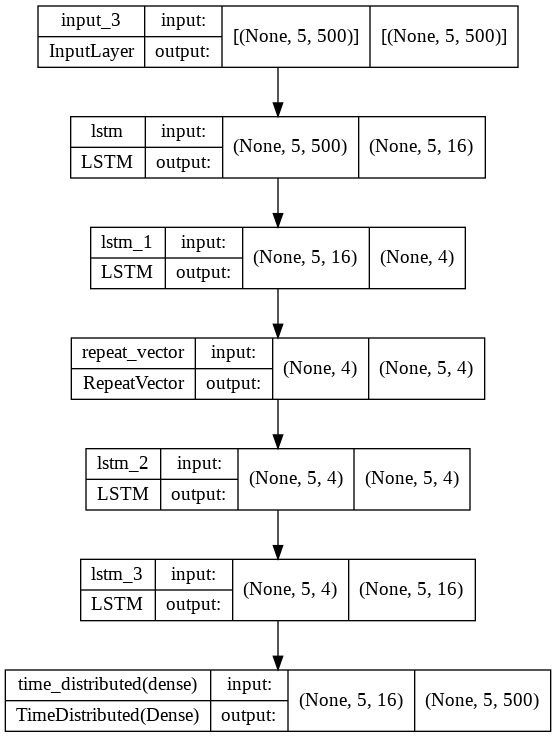
\includegraphics[width=0.85\textwidth]{autoencoder.png}
\caption{Estrutura de um autoencoder: o codificador comprime a entrada até uma
representação latente de baixa dimensão e o decodificador tenta reconstruí-la. A
restrição $d \ll T\cdot S$ força a rede a reter apenas os fatores de variação mais
relevantes.}
\label{fig:profundo-ae}
\end{figure}

A restrição dimensional é o que dá poder ao mecanismo. Como $\vect{z}$ não tem
capacidade para armazenar a entrada integralmente, o treinamento força a retenção dos
fatores de variação mais frequentes. Se o treinamento usa apenas dados normais, esses
fatores são os da normalidade, e a reconstrução de uma entrada anômala é ruim por
construção.

\begin{definicao}{Escore de anomalia por reconstrução}
Dado um autoencoder treinado sobre dados normais,
\begin{equation}
  a(\mat{X}) = \mathcal{D}\big( \mat{X},\; h_{\psi}(g_{\phi}(\mat{X})) \big),
  \label{eq:score-recon}
\end{equation}
e declara-se anomalia quando $a(\mat{X}) > \tau$. O limiar é tipicamente estimado a
partir da distribuição de $a$ sobre dados normais, na forma $\tau = \mu_a + k\sigma_a$.
\end{definicao}

O \cref{cap:dual} usa $\mathcal{D} = \text{SMAPE}$ e $k = 3$. O \cref{cap:mahalanobis}
abandona esse escore em favor da distância no espaço latente, e o motivo será
desenvolvido lá: um autoencoder treinado para reconstruir pode reconstruir bem demais,
inclusive anomalias, quando sua capacidade é suficiente.

\subsection{Autoencoder variacional}

O \termo{autoencoder variacional}{variational autoencoder} (VAE) \citep{VAE,Kingma2014}
substitui o vetor latente determinístico por uma distribuição. O codificador produz
$\vect{\mu}(\mat{X})$ e $\vect{\sigma}(\mat{X})$, amostra-se
$\vect{z} \sim \mathcal{N}(\vect{\mu}, \operatorname{diag}(\vect{\sigma}^2))$ pelo
truque de reparametrização, e acrescenta-se à perda um termo de divergência de
Kullback-Leibler que puxa a posterior aproximada para uma normal padrão:
\begin{equation}
  \mathcal{L}_{\text{VAE}} = \underbrace{\E_{q}\big[ -\log p(\mat{X} \mid \vect{z}) \big]}_{\text{reconstrução}}
  + \beta\, \underbrace{D_{\mathrm{KL}}\big( q(\vect{z}\mid\mat{X}) \,\|\, \mathcal{N}(\vect{0}, \mat{I}) \big)}_{\text{regularização}}.
  \label{eq:vae}
\end{equation}

O efeito é um espaço latente contínuo e suave. A expectativa natural seria que isso
melhorasse o agrupamento subsequente; o \cref{cap:mundoaberto} mostra que não melhorou:
$0{,}727$ contra $0{,}730$ do autoencoder determinístico, diferença sem significância.

\subsection{Rede de agrupamento profundo}

A \termo{rede de agrupamento profundo}{deep clustering network} (DCN) \citep{DCN} otimiza
simultaneamente reconstrução e uma perda de agrupamento no espaço latente:
\begin{equation}
  \mathcal{L}_{\text{DCN}} = \mathcal{L}_{\text{recon}} +
  \lambda \sum_{i} \big\| \vect{z}_i - \vect{c}_{\pi(i)} \big\|^2,
  \label{eq:dcn}
\end{equation}
onde $\vect{c}_{\pi(i)}$ é o centroide atribuído a $\vect{z}_i$. A intenção é produzir
um espaço latente com agrupamentos bem separados. No \cref{cap:mundoaberto}, obteve
$0{,}725$ --- também sem ganho.

\begin{figure}[htbp]
\centering
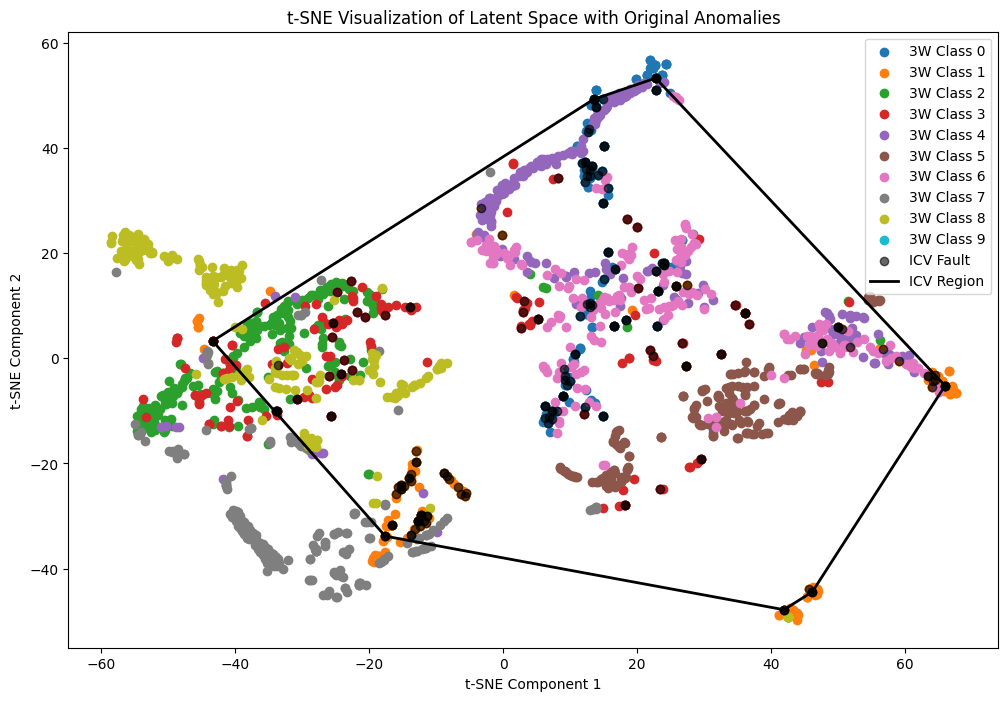
\includegraphics[width=0.72\textwidth]{DCN_latent.png}
\caption{Projeção t-SNE do espaço latente produzido por uma DCN. Cada cor é uma classe
conhecida; o polígono destaca a região ocupada pelas janelas da falha de ICV, uma classe
que a rede nunca viu. Os pontos novos são absorvidos pelos agrupamentos existentes em vez
de formar um agrupamento próprio.}
\label{fig:profundo-dcn}
\end{figure}

A \cref{fig:profundo-dcn} mostra por que o ganho não aparece --- e o motivo é mais
interessante que a ausência de ganho. A perda de agrupamento da \cref{eq:dcn} pune
explicitamente pontos distantes de qualquer centroide. Diante de uma classe nunca vista,
a rede faz exatamente o que foi instruída a fazer: puxa os pontos novos para dentro dos
agrupamentos que já conhece.

\begin{destaque}[Regularizar o latente pode ser contraproducente]
Autoencoder, VAE e DCN diferem justamente em quanto impõem estrutura ao espaço latente ---
nenhuma, gaussiana e por agrupamentos, respectivamente. Para reconstruir, mais estrutura
ajuda. Para \emph{detectar o desconhecido}, ela atrapalha.

O autoencoder simples reconstrói mal o que nunca viu, e essa incompetência é útil: joga
os pontos novos para as bordas do latente, onde são fáceis de isolar. O VAE os
regulariza para junto dos conhecidos; a DCN os absorve nos agrupamentos. Ambos apagam o
sinal que se queria capturar.

É um caso raro em que a propriedade desejável de um modelo é a sua fragilidade.
\end{destaque}

\begin{destaque}[Um resultado negativo instrutivo]
Três variantes de autoencoder, três resultados indistinguíveis: $0{,}730$, $0{,}727$ e
$0{,}725$. A conclusão do \cref{cap:mundoaberto} é que a escolha da variante não era o
gargalo. O gargalo estava no \emph{objetivo}: todas as três otimizam reconstrução, e
reconstrução não é discriminação.

O \cref{cap:mahalanobis} testa a hipótese oposta --- extrair a representação da camada
penúltima de um classificador multiclasse, treinado com objetivo discriminativo --- e
obtém uma melhora de outra ordem de grandeza: índice de silhueta de $0{,}2299$ contra
$-0{,}0149$, e razão de separação de até 186,5 vezes contra menos de 2,5.
\end{destaque}

\section{A U-Net unidimensional}

A U-Net \citep{Ronneberger2015} foi proposta para segmentação de imagens biomédicas e
adaptada aqui para segmentação de séries temporais. Sua estrutura tem três partes.

\begin{description}[leftmargin=0pt,style=nextline,itemsep=0.4em]

\item[Caminho de contração.] Blocos de convolução seguidos de subamostragem. A cada
bloco, a resolução temporal cai pela metade e o número de canais dobra. Captura contexto
progressivamente mais amplo.

\item[Caminho de expansão.] Blocos de superamostragem seguidos de convolução, que
restauram a resolução original.

\item[Conexões de atalho.] Cada nível do caminho de expansão recebe, por concatenação, o
mapa de ativação do nível correspondente do caminho de contração.

\end{description}

\begin{destaque}[Por que as conexões de atalho são o ponto principal]
Sem elas, a informação de localização precisa seria destruída pelas subamostragens
sucessivas: a rede saberia \emph{que} há uma anomalia na janela, mas não \emph{onde} ela
começa. As conexões de atalho reinjetam, em alta resolução, exatamente essa informação.

Para segmentação temporal de eventos de poço, isso é a diferença entre ``esta janela de
duzentos segundos contém um evento'' e ``o evento começa no segundo 137''. A segunda
resposta é a que o operador precisa.
\end{destaque}

A instanciação concreta, com dois níveis, núcleos de tamanho 5 e 32, 64 e 128 canais, é
detalhada no \cref{cap:segmentacao}.

\section{Atenção e Transformers}

O mecanismo de \termo{atenção}{attention} \citep{Vaswani2017} calcula, para cada
posição, uma combinação ponderada de todas as posições da sequência:
\begin{equation}
  \text{Atenção}(\mat{Q}, \mat{K}, \mat{V}) =
  \operatorname{softmax}\!\left( \frac{\mat{Q}\mat{K}^{\top}}{\sqrt{d_k}} \right) \mat{V},
  \label{eq:atencao}
\end{equation}
onde $\mat{Q}$, $\mat{K}$ e $\mat{V}$ --- consultas, chaves e valores --- são projeções
lineares da entrada. Ao contrário da recorrência, o caminho entre duas posições
quaisquer tem comprimento constante, o que elimina o problema do gradiente evanescente
por outra via. O custo é quadrático em $T$.

Nenhum dos modelos treinados neste livro é um Transformer. Ele aparece, contudo, de
forma decisiva: o modelo de linguagem da \cref{parte:explicabilidade} é um Transformer
com centenas de bilhões de parâmetros, e compreender a \cref{eq:atencao} é pré-requisito
para entender o que ele faz e o que ele não faz. Essa discussão é o objeto do
\cref{cap:llm}.

\begin{destaque}[Prática]
O caderno \texttt{3\_introduction\_to\_unsupervised\_learning}, descrito no
\cref{cap:pratica}, treina um autoencoder LSTM sobre janelas do 3W e usa o erro de
reconstrução como escore de anomalia \citep{Lopes2026Intro3W}. Suas escolhas de
estabilidade numérica --- ativação \texttt{tanh}, inicialização ortogonal e recorte de
gradiente --- tornam concreto por que treinar recorrentes sobre sequências longas exige
cuidados que redes densas dispensam.
\end{destaque}

\resumocapitulo{%
As arquiteturas empregadas neste livro formam um repertório pequeno e bem delimitado.
Camadas densas fornecem os classificadores binários. Células LSTM, com seu estado de
célula propagado por soma, tornam viável o processamento de janelas de centenas de
amostras e sustentam os autoencoders recorrentes dos
\cref{cap:dual,cap:mundoaberto,cap:mahalanobis}. Convoluções unidimensionais, com pesos
compartilhados no tempo e campo receptivo controlado pela profundidade e pela
subamostragem, sustentam a U-Net de segmentação do \cref{cap:segmentacao}, cujas
conexões de atalho preservam a informação de localização temporal. Autoencoders
comprimem a entrada em uma representação latente e permitem detectar anomalias por erro
de reconstrução; suas variantes variacional e de agrupamento profundo não produziram
ganho mensurável, o que indica que o gargalo estava no objetivo de reconstrução e não na
arquitetura. O mecanismo de atenção, embora não treinado aqui, é a base dos modelos de
linguagem da Parte IV.}

\begin{exercicios}
\item Calcule o número de parâmetros de uma camada LSTM com $n_h$ unidades recebendo
      entrada de dimensão $n_x$. Aplique ao codificador do \cref{cap:mahalanobis}
      (LSTM(256) seguido de LSTM(128), entrada de 4 canais) e compare com o número de
      parâmetros de um MLP de mesma capacidade de saída sobre a entrada achatada de
      \num{800} dimensões.

\item Mostre, a partir da \cref{eq:lstm-cell}, que quando $\vect{f}_t = \vect{1}$ e
      $\vect{i}_t = \vect{0}$ para todo $t$ em um intervalo, o gradiente de
      $\vect{c}_{t_2}$ em relação a $\vect{c}_{t_1}$ é a identidade. Explique por que
      esse é o mecanismo que resolve o gradiente evanescente.

\item Calcule o campo receptivo de uma pilha de quatro convoluções unidimensionais com
      núcleo 3 e dilatação $1, 2, 4, 8$. Compare com quatro convoluções de núcleo 3 sem
      dilatação. Discuta quando convoluções dilatadas seriam preferíveis à subamostragem
      da U-Net.

\item Um autoencoder com $d = T \cdot S$ pode aprender a função identidade e ter erro de
      reconstrução nulo para qualquer entrada, inclusive anômala. Discuta três formas de
      impedir isso além da redução de $d$, e relacione cada uma a um mecanismo de
      regularização apresentado neste capítulo.

\item Derive a \cref{eq:vae} a partir do limite inferior da evidência (ELBO). Explique
      qual o papel do coeficiente $\beta$ e o que acontece nos limites $\beta \to 0$ e
      $\beta \to \infty$.

\item Implemente uma U-Net unidimensional com dois níveis e treine-a para segmentar
      regiões anômalas em uma instância sintética. Em seguida, remova as conexões de
      atalho, retreine e compare o IOU. Quantifique a degradação.

\item A complexidade da atenção é $O(T^2 d)$. Para $T = \num{86400}$ (um dia a
      \SI{1}{\hertz}) e $d = 128$, estime o número de operações de uma única camada de
      atenção. Discuta por que isso inviabiliza a aplicação direta de Transformers a
      séries temporais brutas de poço e cite duas estratégias da literatura para
      contornar o problema.
\end{exercicios}

\begin{leituras}
\item \citet{Hochreiter1997} --- artigo original da LSTM. Denso, mas a
      \cref{eq:lstm-cell} fica muito mais clara depois de lê-lo.
\item \citet{SCHMIDHUBER201585} --- panorama histórico do aprendizado profundo, útil
      para situar cada arquitetura em sua motivação original.
\item \citet{Ronneberger2015} --- a U-Net. A figura em forma de U do artigo é uma das
      mais reproduzidas da área, e por bons motivos.
\item \citet{Vaswani2017} --- o Transformer.
\item \citet{Kingma2014} e \citet{VAE} --- autoencoders variacionais.
\item \citet{srivastava14a} --- \ing{dropout}, com a análise que justifica sua
      interpretação como \ing{ensemble} implícito.
\end{leituras}

\chapter{Detecção de novidade e mundo aberto}
\label{cap:novidades}

\begin{objetivos}
Ao final deste capítulo, você será capaz de:
\begin{itemize}[leftmargin=*,itemsep=0.2em]
  \item distinguir formalmente classificação de mundo fechado, reconhecimento em
        conjunto aberto e aprendizado de mundo aberto;
  \item calcular o risco de espaço aberto e explicar por que classificadores
        discriminativos convencionais o ignoram;
  \item comparar quatro famílias de escore de novidade --- erro de reconstrução,
        máquina de vetores de suporte de uma classe, distância de Mahalanobis e
        rejeição por ensemble binário --- e discutir critérios para escolher entre elas;
  \item enunciar as hipóteses que K-means, MeanShift e DBSCAN fazem sobre os dados e
        comparar sua adequação a partir dessas hipóteses;
  \item avaliar a qualidade de um agrupamento sem rótulos usando os índices de silhueta,
        Davies-Bouldin e Calinski-Harabasz;
  \item interpretar projeções de PCA, t-SNE e UMAP, reconhecendo os limites de cada uma.
\end{itemize}
\end{objetivos}

\section{Três níveis de abertura}

\begin{definicao}{Classificação de mundo fechado}
Dado um conjunto de classes conhecidas $\mathcal{K} = \{1, \dots, K\}$, busca-se
$f: \mathcal{X} \to \mathcal{K}$. Pressupõe-se que toda entrada pertence a
$\mathcal{K}$.
\end{definicao}

\begin{definicao}{Reconhecimento em conjunto aberto}
Busca-se $f: \mathcal{X} \to \mathcal{K} \cup \{\texttt{desconhecido}\}$. O sistema pode
recusar-se a classificar, mas não faz nada com o que recusou \citep{Scheirer2013}.
\end{definicao}

\begin{definicao}{Aprendizado de mundo aberto}
Além de recusar, o sistema \emph{agrupa} as instâncias rejeitadas, propõe novas classes,
submete-as a validação e incorpora as validadas a $\mathcal{K}$, de modo que
$\mathcal{K}_{t+1} \supseteq \mathcal{K}_{t}$. O ciclo se repete indefinidamente.
\end{definicao}

Os três níveis correspondem, quase exatamente, aos capítulos da \cref{parte:base}: o
\cref{cap:dual} opera em mundo fechado com um mecanismo de detecção acoplado; o
\cref{cap:binarios} realiza reconhecimento em conjunto aberto; o \cref{cap:mundoaberto}
fecha o ciclo completo de aprendizado de mundo aberto.

\subsection{Risco de espaço aberto}

\citet{Scheirer2013} formalizam por que classificadores discriminativos falham em
conjunto aberto. Seja $f$ uma função de decisão para a classe $k$ e seja
$\mathcal{S}_o$ uma região limitada do espaço de características contendo todos os
exemplos de treinamento. Define-se o \termo{risco de espaço aberto}{open space risk}
como
\begin{equation}
  R_{\mathcal{O}}(f) = \frac{\displaystyle\int_{\mathcal{O}} f(\vect{x})\, d\vect{x}}
                             {\displaystyle\int_{\mathcal{S}_o} f(\vect{x})\, d\vect{x}},
  \label{eq:open-space-risk}
\end{equation}
onde $\mathcal{O} = \mathcal{S}_o \setminus \mathcal{S}_{\text{treino}}$ é o espaço
aberto --- a região do espaço de características arbitrariamente longe de qualquer
exemplo visto.

A leitura é simples e devastadora. Um hiperplano separador, como o de uma regressão
logística ou de uma SVM linear, produz $f(\vect{x}) = 1$ em um semiespaço \emph{de
volume infinito}. Seu risco de espaço aberto é ilimitado: existem regiões
arbitrariamente distantes de qualquer dado de treinamento em que o modelo declara,
com confiança máxima, pertinência à classe.

Essa conclusão se aplica a funções de decisão cuja região positiva é não limitada,
como o hiperplano linear deste exemplo; não é uma propriedade automática de todo modelo
discriminativo, pois arquitetura e regra de decisão podem produzir regiões limitadas.

\begin{destaque}[A geometria da rejeição]
A conclusão prática é que \emph{funções de decisão que declaram pertinência devem ser
limitadas}. As quatro abordagens da \cref{sec:novidades-escores} são, cada uma à sua
maneira, formas de impor essa limitação: uma esfera no espaço latente (Mahalanobis), um
envelope em torno dos dados (OCSVM), um limiar sobre o erro de reconstrução, ou a
conjunção de $K$ decisões binárias independentes.
\end{destaque}

\section{Quatro escores de novidade}
\label{sec:novidades-escores}

\subsection{Erro de reconstrução}

Já apresentado no \cref{cap:profundo}: treina-se um autoencoder sobre dados normais e
usa-se $a(\mat{X}) = \mathcal{D}(\mat{X}, h_{\psi}(g_{\phi}(\mat{X})))$ como escore.

\textbf{Vantagem.} Não requer rótulos de anomalia --- é a única das quatro que
funciona quando não há um único exemplo de anomalia disponível.

\textbf{Desvantagem.} Depende criticamente da capacidade do modelo. Um autoencoder
muito expressivo generaliza demais e reconstrói bem entradas anômalas; um autoencoder
pouco expressivo reconstrói mal tudo. Não há critério simples para acertar o ponto.

\begin{figure}[htbp]
\centering
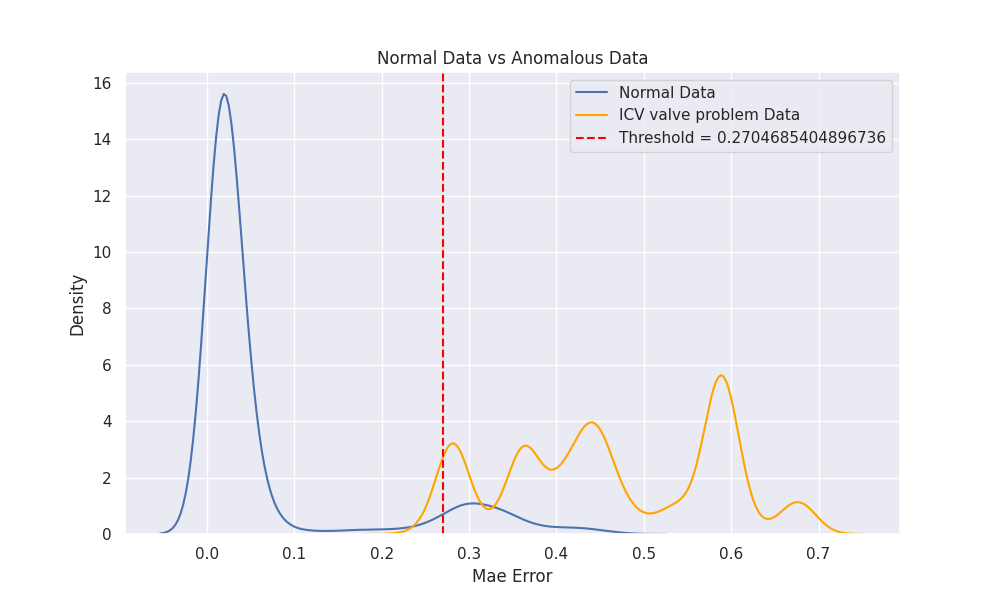
\includegraphics[width=0.86\textwidth]{distribution_comparison.png}
\caption{Densidade interpolada do erro de reconstrução para dados normais e para janelas
de falha de ICV, com o limiar probabilístico assinalado. A área sob cada curva soma um.}
\label{fig:novidades-limiar}
\end{figure}

A \cref{fig:novidades-limiar} mostra o formato típico do problema. As duas distribuições
se sobrepõem, e o limiar é uma linha vertical que escolhe onde pagar o custo: mais à
esquerda, capturam-se quase todas as anomalias ao preço de falsos alarmes; mais à
direita, o oposto.

Essa figura também explica por que a escolha do limiar costuma importar mais que a
escolha da arquitetura. Deslocar a linha percorre toda a curva ROC; trocar o autoencoder
move as duas distribuições apenas alguns por cento uma em relação à outra.

\subsection{Máquina de vetores de suporte de uma classe}

A OCSVM \citep{Smola2004} busca a hiperesfera de raio mínimo (ou o hiperplano de margem
máxima em relação à origem, no espaço de características induzido pelo núcleo) que
contenha uma fração $1 - \nu$ dos dados de treinamento:
\begin{equation}
  \min_{\vect{w}, \rho, \vect{\xi}} \quad
  \frac{1}{2}\|\vect{w}\|^2 + \frac{1}{\nu n}\sum_i \xi_i - \rho
  \quad \text{s.a.} \quad
  \langle \vect{w}, \varphi(\vect{x}_i)\rangle \ge \rho - \xi_i,\ \ \xi_i \ge 0.
  \label{eq:ocsvm}
\end{equation}

\textbf{Vantagem.} Fronteira de decisão limitada por construção; risco de espaço aberto
controlado.

\textbf{Desvantagem.} Escala mal com o número de amostras e é sensível à escolha do
núcleo e de $\nu$. No \cref{cap:closedworld}, uma OCSVM aplicada diretamente aos dados
brutos atinge apenas $0{,}65$ de acurácia global, contra $0{,}87$ do ensemble binário.
A comparação descreve o protocolo daquele capítulo, com representações e objetivos
distintos; não estabelece uma ordenação universal entre OCSVM e ensembles.
A OCSVM reaparece, contudo, no \cref{cap:mundoaberto} como \emph{componente} de um voto
ponderado --- e ali contribui, porque erra de forma diferente do ensemble.

\begin{figure}[htbp]
\centering
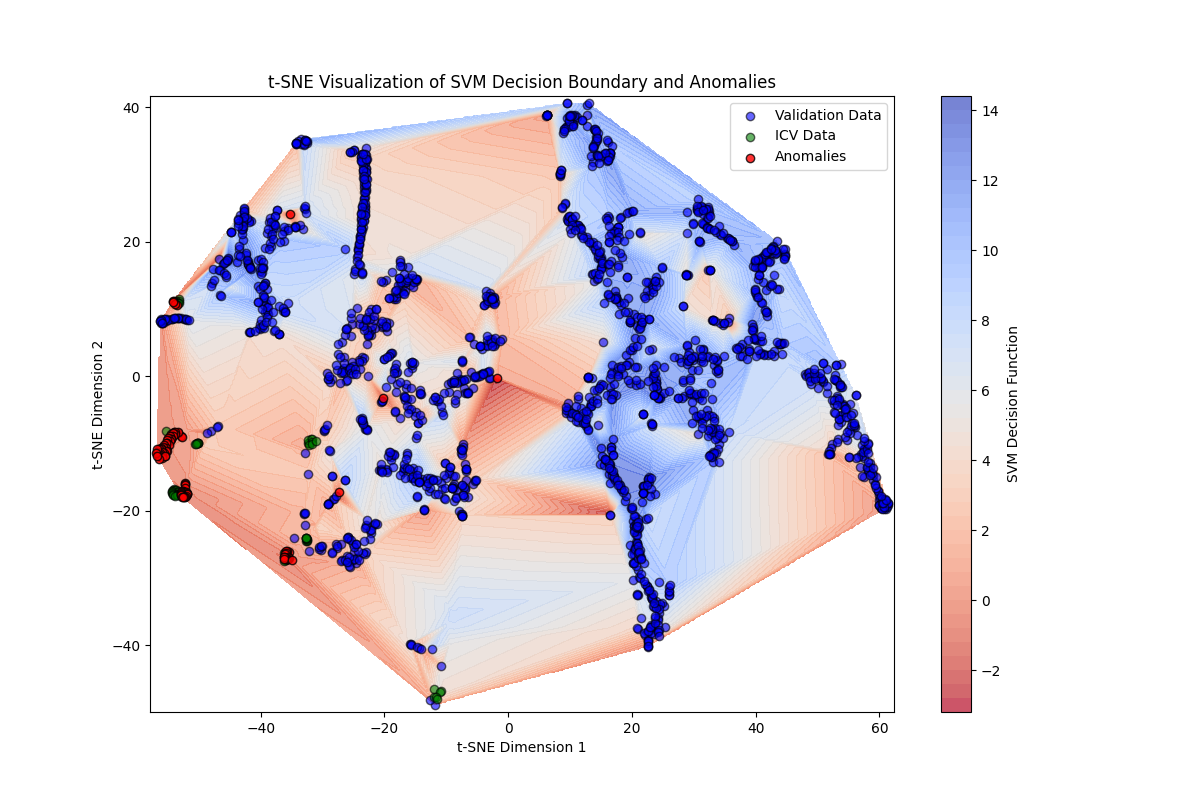
\includegraphics[width=0.86\textwidth]{SVM_Decision.png}
\caption{Fronteira de decisão de uma OCSVM treinada sobre o espaço latente, projetada por
t-SNE. O gradiente representa o valor da função de decisão: regiões escuras são
classificadas com confiança como conhecidas; regiões claras, como não-classe. Os pontos
sobrepostos distinguem dados de validação, dados de ICV e amostras de não-classe.}
\label{fig:novidades-ocsvm}
\end{figure}

A \cref{fig:novidades-ocsvm} torna visível o que a \cref{eq:ocsvm} formaliza: a fronteira
envolve o suporte dos dados conhecidos em vez de separar duas classes. É a diferença
entre \emph{onde os dados estão} e \emph{o que os separa} --- e é exatamente essa
diferença que limita o risco de espaço aberto da \cref{eq:open-space-risk}.

\subsection{Distância de Mahalanobis}

\begin{definicao}{Distância de Mahalanobis}
Para uma distribuição com média $\vect{\mu}$ e covariância $\mat{\Sigma}$,
\begin{equation}
  d_M(\vect{x}) = \sqrt{ (\vect{x} - \vect{\mu})^{\top} \mat{\Sigma}^{-1} (\vect{x} - \vect{\mu}) }.
  \label{eq:mahalanobis}
\end{equation}
\end{definicao}

A distância de Mahalanobis é a distância euclidiana medida no sistema de coordenadas em
que a distribuição é esférica: ela normaliza pela variância em cada direção e
descorrelaciona os eixos. Um ponto a duas unidades de distância ao longo de uma direção
de alta variância é menos surpreendente que um ponto a duas unidades ao longo de uma
direção de baixa variância, e a \cref{eq:mahalanobis} captura exatamente isso.

Em alta dimensão, $\mat{\Sigma}$ é frequentemente mal condicionada ou singular. A
contramedida padrão, adotada no \cref{cap:mahalanobis}, é a regularização
\begin{equation}
  \mat{\Sigma}_{\text{reg}} = \mat{\Sigma} + \lambda \mat{I}.
  \label{eq:sigma-reg}
\end{equation}

\textbf{Vantagem.} Fechada, barata, com uma única hipótese explícita (aproximação
gaussiana por classe) e um limiar natural via quantil da distribuição
$\chi^2$ --- ou, empiricamente, o percentil 95 dos dados de treinamento.

\textbf{Desvantagem.} A hipótese gaussiana. Aplicada ao espaço bruto, ela é
grosseiramente violada, e o desempenho reflete isso. Aplicada a um espaço latente
discriminativo, torna-se aceitável --- e o desempenho salta. Esse é, em uma frase, o
achado central do \cref{cap:mahalanobis}.

\begin{exemplo}{A diferença que o espaço faz}
O \cref{cap:mahalanobis} reporta, para a classe 8 (hidrato na linha de produção), uma
razão de separação --- distância média das instâncias desconhecidas dividida pela
distância média das conhecidas --- de menos de $1{,}0$ no espaço bruto e de
$186{,}5$ no espaço latente do classificador multiclasse.

Não é um ganho incremental. No espaço bruto, as instâncias desconhecidas estão
\emph{mais próximas} do centro da distribuição que as conhecidas: o escore é
anti-informativo. No espaço latente, a separação é tão grande que qualquer limiar
razoável funciona.
\end{exemplo}

\subsection{Rejeição por ensemble binário}

A quarta abordagem é a que dá nome ao \cref{cap:binarios}. Em vez de um classificador
multiclasse, treinam-se $K$ classificadores binários independentes, um por classe, cada
um respondendo ``esta janela é da classe $k$?''. A decisão final é
\begin{equation}
  \hat{y} = \begin{cases}
    \argmax_{k} s_k(\mat{X}), & \text{se } \max_k s_k(\mat{X}) > \tau, \\[0.3em]
    \texttt{desconhecido},    & \text{caso contrário.}
  \end{cases}
  \label{eq:ensemble-rejeicao}
\end{equation}

A diferença em relação a aplicar um limiar sobre a \ing{softmax} de um classificador
multiclasse é estrutural, não cosmética. Os escores $s_k$ são produzidos por modelos
independentes, cada um com sua própria sigmoide, e \emph{não somam um}. Nada impede que
todos sejam simultaneamente baixos --- e ``todos baixos'' é precisamente a assinatura de
uma classe desconhecida.

\begin{destaque}[O preço da independência]
Nove modelos custam nove vezes mais em memória e tempo. O \cref{cap:closedworld}
quantifica: um classificador ocupa cerca de \SI{2,3}{\mega\byte} e leva
\SI{45}{\milli\second} por inferência; o ensemble de nove ocupa \SI{21}{\mega\byte} e
leva \SI{405}{\milli\second}. Para um evento cuja escala característica é de horas, esse
custo é irrelevante --- e é essa observação, e não uma otimização de arquitetura, que
justifica a escolha.
\end{destaque}

\subsection{Comparação}

\begin{center}
\small
\begin{tabular}{p{3.0cm} p{2.4cm} p{3.0cm} p{3.6cm}}
\toprule
\textbf{Escore} & \textbf{Rótulos de anomalia} & \textbf{Hipótese principal} &
\textbf{Onde aparece} \\
\midrule
Reconstrução & Não requer & Anomalia reconstrói mal & \cref{cap:dual},
\cref{cap:mundoaberto} \\
OCSVM        & Não requer & Normalidade é compacta & \cref{cap:mundoaberto},
\cref{cap:closedworld} \\
Mahalanobis  & Requer (por classe) & Gaussiana por classe & \cref{cap:mahalanobis} \\
Ensemble binário & Requer & Classes são separáveis individualmente &
\cref{cap:binarios}, \cref{cap:closedworld} \\
\bottomrule
\end{tabular}
\end{center}

\section{Agrupamento}

Rejeitar é metade do problema. A outra metade --- organizar o que foi rejeitado em
grupos coerentes que possam se tornar classes --- é agrupamento.

\subsection{K-means}

Minimiza a inércia
\begin{equation}
  J = \sum_{i=1}^{n} \big\| \vect{z}_i - \vect{c}_{\pi(i)} \big\|^2,
  \label{eq:kmeans}
\end{equation}
alternando atribuição de pontos a centroides e recálculo de centroides
\citep{Lloyd1982}. Rápido e simples, com duas limitações severas: exige $K$ conhecido a
priori e pressupõe agrupamentos aproximadamente esféricos e de tamanhos comparáveis.

\begin{destaque}[Como o \cref{cap:mundoaberto} resolve o problema do $K$]
Em mundo aberto, $K$ é exatamente a quantidade que não se conhece --- é o número de
classes novas. A solução adotada é original: treina-se uma floresta aleatória para
\emph{prever} $K$ a partir de oito características do próprio conjunto a ser agrupado
(número de pontos, índice de silhueta, Davies-Bouldin, Calinski-Harabasz, inércia, e
três descritores geométricos). \citet{Lopes2025EAAI} reportam $98{,}3\,\%$ de acurácia
e erro médio absoluto de $1{,}12$ para essa etapa. O \cref{cap:mundoaberto} reproduz os
demais indicadores publicados e discute por que esses dois valores não devem ser
interpretados conjuntamente sem confirmar seus denominadores e definições.
\end{destaque}

\subsection{MeanShift}

Desloca iterativamente cada ponto na direção do gradiente estimado da densidade,
convergindo para modos locais \citep{meanshift}. Não exige $K$ --- ele emerge do número
de modos --- mas exige a largura de banda do núcleo, que controla implicitamente a
mesma coisa. É computacionalmente mais caro que o K-means.

\subsection{DBSCAN}

Define agrupamentos como regiões de densidade suficiente, conectando pontos que têm ao
menos \texttt{minPts} vizinhos em raio $\varepsilon$ \citep{dbscan}. Duas propriedades o
distinguem: encontra agrupamentos de forma arbitrária, e classifica explicitamente
pontos de baixa densidade como \emph{ruído}.

A segunda propriedade é atraente em mundo aberto --- rejeitar é desejável --- mas tem um
custo: em espaços de alta dimensão, a noção de densidade se degrada e o DBSCAN tende a
classificar quase tudo como ruído. É o motivo pelo qual o \cref{cap:mundoaberto} o usa
apenas como comparação, e não como componente do pipeline.

\subsection{Combinação e refinamento}

O \cref{cap:mundoaberto} não escolhe um algoritmo: executa K-means e MeanShift e
\emph{intersecta} os resultados, mantendo apenas os pontos em que ambos concordam.
Aplica em seguida um refinamento por limiar adaptativo, no qual pontos distantes do
centroide são removidos com um multiplicador $k$ que depende da razão
$R = \mu/\sigma$ das distâncias intra-agrupamento:
\begin{equation}
  k = \begin{cases}
    2, & R \ge 4, \\
    1 + \dfrac{R - 2}{2}, & 2 \le R < 4, \\
    0, & R < 2.
  \end{cases}
  \label{eq:limiar-adaptativo}
\end{equation}

A intuição: quando as distâncias são concentradas ($R$ alto), o agrupamento é coeso e
pode-se ser tolerante; quando são dispersas ($R$ baixo), o agrupamento é duvidoso e
convém ser agressivo na remoção. Uma salvaguarda impede que mais de um terço dos pontos
seja descartado.

\section{Avaliar agrupamentos sem rótulos}

Três índices internos são usados neste livro.

\begin{definicao}{Índice de silhueta}
Para cada ponto $i$, sejam $a(i)$ a distância média aos pontos do próprio agrupamento e
$b(i)$ a menor distância média aos pontos de outro agrupamento. Então
\begin{equation}
  s(i) = \frac{b(i) - a(i)}{\max\{a(i), b(i)\}} \in [-1, 1],
  \label{eq:silhueta}
\end{equation}
e o índice global é a média sobre todos os pontos \citep{Rousseeuw1987}. Valores
próximos de $1$ indicam agrupamentos bem separados; próximos de $0$, sobreposição;
negativos, atribuição incorreta.
\end{definicao}

\begin{definicao}{Índice de Davies-Bouldin}
\begin{equation}
  \text{DB} = \frac{1}{K}\sum_{i=1}^{K} \max_{j \ne i}
  \frac{\sigma_i + \sigma_j}{d(\vect{c}_i, \vect{c}_j)},
  \label{eq:db}
\end{equation}
onde $\sigma_i$ é a dispersão média do agrupamento $i$. \emph{Menor é melhor.}
\end{definicao}

\begin{definicao}{Índice de Calinski-Harabasz}
Razão entre dispersão entre agrupamentos e dispersão intra-agrupamento, normalizada
pelos graus de liberdade \citep{Calinski1974}. \emph{Maior é melhor.}
\end{definicao}

\begin{exemplo}{Os três índices concordando}
O \cref{cap:mahalanobis} compara o espaço latente de um autoencoder com o de um
classificador multiclasse:

\begin{center}
\small
\begin{tabular}{lrr}
\toprule
\textbf{Índice} & \textbf{Latente do AE} & \textbf{Latente multiclasse} \\
\midrule
Silhueta (maior é melhor)          & $-0{,}0149$ & $0{,}2299$ \\
Calinski-Harabasz (maior é melhor) & $687{,}8008$ & $2818{,}2310$ \\
Davies-Bouldin (menor é melhor)    & $4{,}5592$  & $1{,}7460$ \\
\bottomrule
\end{tabular}
\end{center}

Os três índices, que medem coisas diferentes e podem discordar, apontam na mesma
direção. Quando isso acontece, a conclusão é robusta.
\end{exemplo}

\begin{destaque}[Índices internos não substituem rótulos]
Todo índice interno mede coerência geométrica, não correção semântica. Um agrupamento
com silhueta $0{,}9$ pode separar perfeitamente dois poços em vez de duas anomalias.
É por isso que o pipeline do \cref{cap:mundoaberto} termina com validação por
especialista, e por isso que o \cref{cap:agente} propõe usar um modelo de linguagem
para \emph{nomear} os agrupamentos --- transformando geometria em hipótese
interpretável.
\end{destaque}

\section{Visualização}

Três técnicas de redução de dimensionalidade são usadas para inspeção.

\begin{description}[leftmargin=0pt,style=nextline,itemsep=0.4em]

\item[PCA.] Projeção linear nas direções de maior variância. Preserva distâncias globais
e é determinística e interpretável. Falha quando a estrutura é não linear.

\item[t-SNE.] Preserva vizinhanças locais minimizando a divergência entre distribuições
de similaridade no espaço original e no reduzido \citep{maaten2008visualizing}.
Excelente para revelar agrupamentos; \emph{as distâncias entre agrupamentos no gráfico
não têm significado}, e o resultado depende da perplexidade e da semente aleatória.

\item[UMAP.] Baseia-se em geometria riemanniana e topologia algébrica; preserva melhor a
estrutura global que o t-SNE e é mais rápido. Compartilha, contudo, a mesma limitação:
é uma ferramenta de inspeção, não de medida.

\end{description}

\begin{destaque}[Regra de uso]
Nenhuma conclusão quantitativa deste livro se apoia em uma projeção bidimensional.
As projeções aparecem para \emph{ilustrar} uma conclusão já estabelecida por índices
numéricos. A inversão dessa ordem --- olhar a projeção, ver agrupamentos, concluir que
existem --- é um dos erros mais comuns na aplicação de aprendizado não supervisionado.
\end{destaque}

\section{O ciclo completo}

Reunindo as peças, o aprendizado de mundo aberto pode ser enunciado como um ciclo de
seis estágios, que é exatamente a estrutura do \cref{cap:mundoaberto}:

\begin{figure}[htbp]
\centering
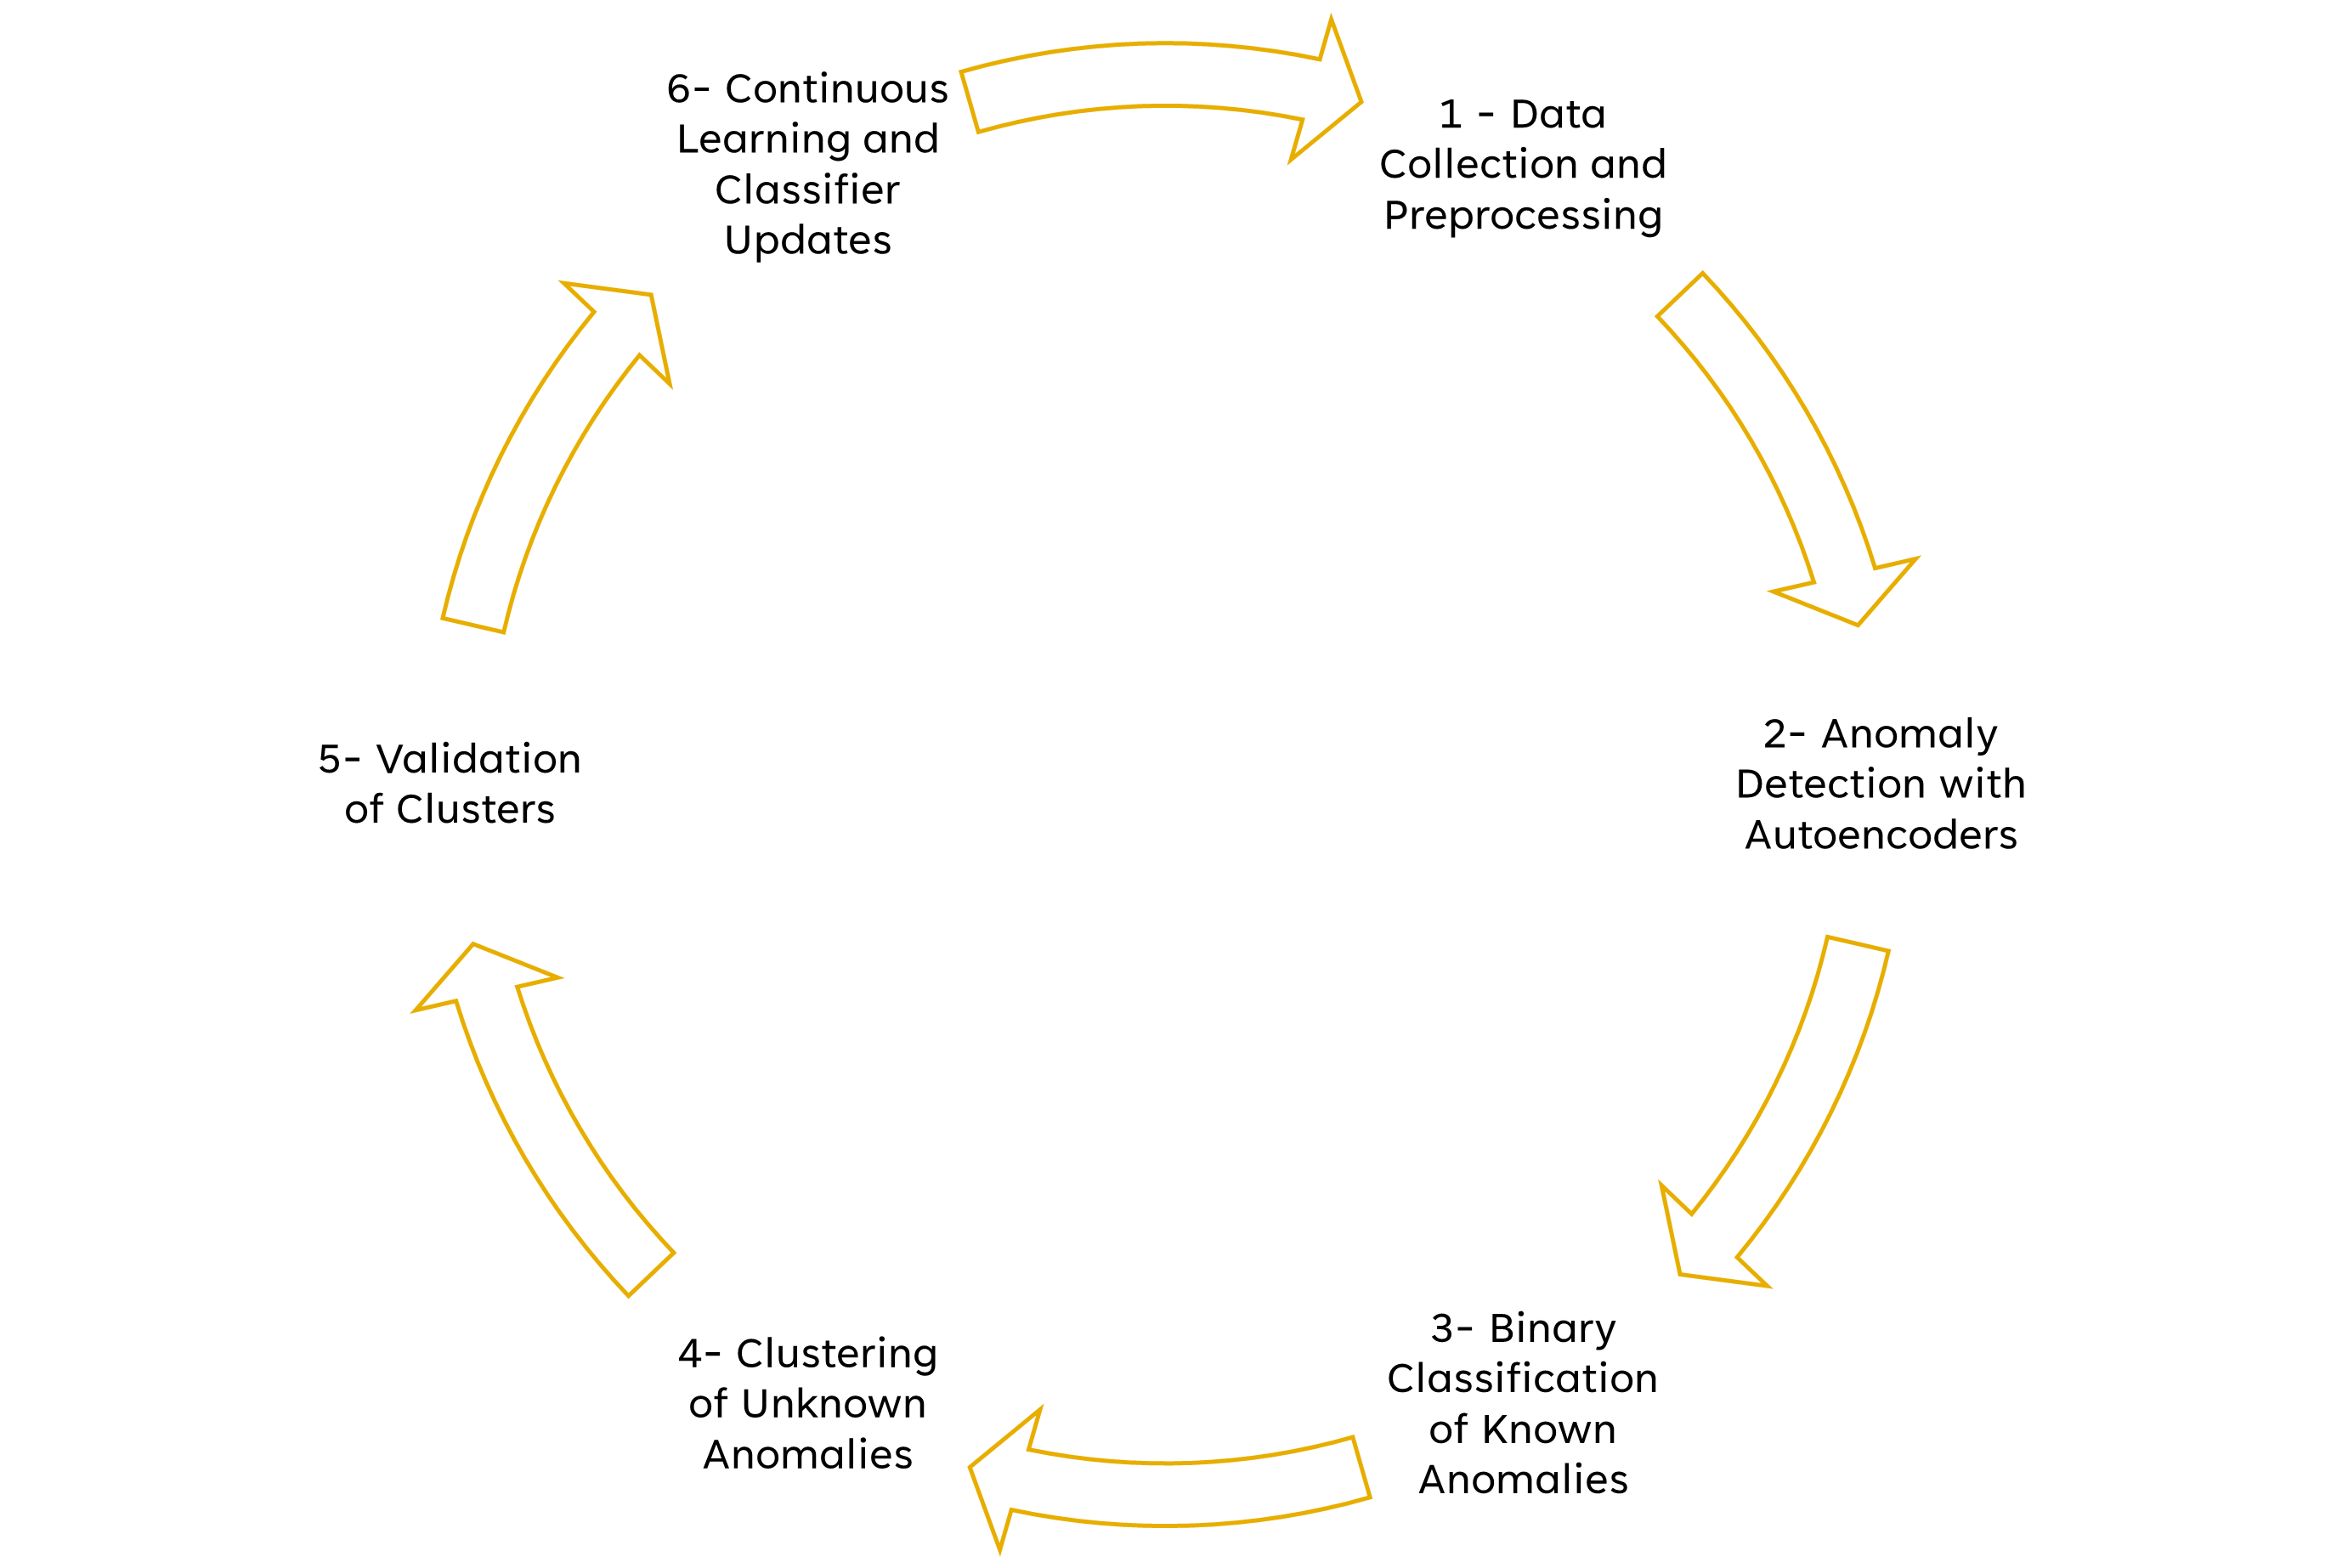
\includegraphics[width=0.78\textwidth]{general_method.png}
\caption{O ciclo de aprendizado de mundo aberto aplicado à operação de poços. O fluxo é
fechado: o conhecimento validado ao fim de uma volta passa a integrar a base de
classificadores usada na volta seguinte.}
\label{fig:novidades-ciclo}
\end{figure}

\begin{enumerate}[leftmargin=*,itemsep=0.3em]
  \item \textbf{Representar.} Mapear a janela bruta em um espaço latente
        ($\vect{z} = g_{\phi}(\mat{X})$).
  \item \textbf{Classificar.} Aplicar os classificadores da base de conhecimento atual.
  \item \textbf{Rejeitar.} Marcar como desconhecido aquilo que nenhum classificador
        reivindica com confiança suficiente.
  \item \textbf{Agrupar.} Organizar o material rejeitado em grupos coerentes,
        estimando o número de grupos.
  \item \textbf{Validar.} Submeter os grupos a um especialista --- humano ou, como
        propõe a \cref{parte:explicabilidade}, um agente de linguagem que produza uma
        hipótese nomeada e justificada.
  \item \textbf{Incorporar.} Treinar um novo classificador binário para cada grupo
        validado e adicioná-lo ao ensemble, sem retreinar os existentes.
\end{enumerate}

O sexto estágio merece destaque. Como os classificadores são binários e independentes,
acrescentar uma classe custa \emph{um} treinamento, e não o retreinamento de todo o
sistema. Essa propriedade --- consequência direta da escolha arquitetural do
\cref{cap:binarios} --- é o que torna o ciclo operacionalmente viável.

A \cref{fig:novidades-ciclo} representa o mesmo processo em forma de diagrama, e a
representação circular não é ornamental: ela afirma que não existe um estado final. Cada
volta amplia o conjunto de classes conhecidas, e o mundo aberto de hoje é o mundo fechado
de amanhã --- até que a próxima anomalia inédita apareça.

\begin{destaque}[Prática]
Os cadernos \texttt{2\_visualization\_techniques} e \texttt{5\_clustering\_methods},
descritos no \cref{cap:pratica}, cobrem os dois estágios centrais deste ciclo
\citep{Lopes2026Intro3W}. O primeiro mostra, com quatro configurações de t-SNE e quatro
de UMAP sobre os mesmos dados, por que a projeção é uma escolha e não uma medida. O
segundo aplica $K$-médias, DBSCAN e MeanShift com silhueta e índice de Rand ajustado, e
reproduz em escala reduzida a dificuldade que estrutura o \cref{cap:mundoaberto}.
\end{destaque}

\resumocapitulo{%
A hipótese de mundo fechado é uma escolha, não uma necessidade. O reconhecimento em
conjunto aberto permite recusar-se a classificar; o aprendizado de mundo aberto vai
além e transforma o recusado em novo conhecimento. O risco de espaço aberto explica
formalmente por que fronteiras de decisão ilimitadas --- hiperplanos, \ing{softmax} ---
falham nesse cenário: elas declaram pertinência com confiança máxima em regiões
arbitrariamente distantes de qualquer dado visto. Quatro famílias de escore de novidade
impõem limitação de formas distintas: erro de reconstrução, OCSVM, distância de
Mahalanobis e rejeição por ensemble de classificadores binários. O material rejeitado é
organizado por agrupamento --- K-means, MeanShift, DBSCAN --- cuja qualidade se avalia
por índices internos de silhueta, Davies-Bouldin e Calinski-Harabasz. Índices internos e
projeções bidimensionais medem coerência geométrica, jamais correção semântica; a
validação exige um especialista, e é essa lacuna que a Parte IV se propõe a preencher.}

\begin{exercicios}
\item Considere um classificador linear binário em $\R^2$ com fronteira
      $w_1 x_1 + w_2 x_2 + b = 0$. Mostre que a região classificada como positiva tem
      área infinita e conclua que seu risco de espaço aberto, conforme a
      \cref{eq:open-space-risk}, é ilimitado. Em seguida, mostre que uma esfera de raio
      finito tem risco limitado.

\item Demonstre que, quando $\mat{\Sigma} = \sigma^2\mat{I}$, a distância de Mahalanobis
      reduz-se à distância euclidiana dividida por $\sigma$. Interprete geometricamente o
      papel de $\mat{\Sigma}^{-1}$ no caso geral.

\item Explique por que os escores de $K$ classificadores binários independentes não somam
      um, e por que isso é exatamente a propriedade necessária para expressar ``nenhuma
      das anteriores''. Em seguida, discuta o que acontece quando dois classificadores
      reivindicam a mesma janela com escores altos.

\item Implemente o limiar adaptativo da \cref{eq:limiar-adaptativo} e aplique-o a
      agrupamentos sintéticos com diferentes razões $R = \mu/\sigma$. Verifique
      empiricamente se a salvaguarda de um terço é acionada e em que condições.

\item Gere dois conjuntos bidimensionais: um com dois agrupamentos gaussianos bem
      separados, outro com dois anéis concêntricos. Aplique K-means, MeanShift e DBSCAN
      a ambos e calcule os três índices internos. Discuta em quais casos os índices
      concordam com a estrutura verdadeira e em quais não.

\item O estimador de $K$ do \cref{cap:mundoaberto} usa oito características, entre elas
      os próprios índices de silhueta, Davies-Bouldin e Calinski-Harabasz. Explique por
      que isso não é circular. Proponha duas características adicionais que poderiam
      melhorar o estimador.

\item Discuta a seguinte objeção ao ciclo de seis estágios: ``se o especialista precisa
      validar cada grupo, o sistema não é autônomo e o ganho é ilusório''. Formule uma
      resposta quantitativa em termos do número de decisões que o especialista precisaria
      tomar com e sem o sistema.
\end{exercicios}

\begin{leituras}
\item \citet{Scheirer2013} --- a formalização do conjunto aberto e do risco de espaço
      aberto.
\item \citet{Pimentel2014review} --- revisão abrangente de detecção de novidade,
      organizada por família de método.
\item \citet{Smola2004} --- fundamentação da OCSVM.
\item \citet{Rousseeuw1987}, \citet{Calinski1974} --- índices de validação de
      agrupamento.
\item \citet{dbscan} e \citet{meanshift} --- os algoritmos originais.
\item \citet{maaten2008visualizing} --- t-SNE, com discussão honesta de suas limitações.
\end{leituras}


\part{A base: da regra ao mundo aberto}\label{parte:base}
\chapter{O sistema dual: regra e reconstrução}
\label{cap:dual}

\begin{objetivos}
Ao final deste capítulo, você será capaz de:
\begin{itemize}[leftmargin=*,itemsep=0.2em]
  \item descrever a arquitetura de um sistema dual que combina um diagrama de decisão
        determinístico com um autoencoder recorrente;
  \item justificar por que a combinação supera cada componente isolado, em termos de
        cobertura e de taxa de falsos positivos;
  \item descrever as decisões de projeto de um autoencoder LSTM para detecção de
        anomalias e a definição de seu limiar pela regra $\mu + 3\sigma$;
  \item explicar como o sistema se autotreina em campo, sem rotulação humana, e quais
        salvaguardas isso exige;
  \item interpretar os resultados de três estudos de caso reais e compará-los com a
        literatura sobre fechamento espúrio de DHSV.
\end{itemize}
\end{objetivos}

\section{O problema que este capítulo resolve}

Comecemos pelo requisito, não pelo método.

Uma operadora deseja monitorar duzentos e cinquenta poços submarinos em tempo real.
Cada poço tem um comportamento distinto: níveis de pressão diferentes, curvas de
declínio diferentes, esquemas de elevação artificial diferentes. Não há rotulação
humana disponível de forma contínua. Não há garantia de que os eventos que ocorrerão
estejam catalogados. E o sistema precisa funcionar a partir do momento em que é ligado.

Essas quatro restrições eliminam, de saída, a solução acadêmica padrão --- treinar um
classificador supervisionado sobre um conjunto rotulado e implantá-lo. O que se propõe
neste capítulo, e que efetivamente opera em campo, é uma arquitetura de dois
componentes com naturezas complementares.

\begin{description}[leftmargin=0pt,style=nextline,itemsep=0.5em]

\item[Um diagrama de decisão determinístico.] Codifica conhecimento de engenharia em
regras explícitas. Não requer treinamento, funciona no primeiro segundo, é auditável e
seu comportamento é previsível. Em contrapartida, só reconhece o que foi explicitamente
programado.

\item[Um autoencoder recorrente.] Aprende o comportamento normal \emph{daquele poço
específico} a partir dos próprios dados, sem rótulos, e sinaliza qualquer desvio.
Detecta o inesperado, mas não sabe nomeá-lo e precisa de tempo para aprender.

\end{description}

\begin{destaque}[A tese deste capítulo]
Os dois componentes não competem: eles se alimentam. O diagrama de decisão determina
\emph{quais dados são normais} e, com isso, fornece ao autoencoder o conjunto de
treinamento que ele não teria de outra forma. O autoencoder, por sua vez, cobre o
espaço de eventos que o diagrama não enumera. É uma relação de mão dupla, e é essa
relação que produz o ganho de desempenho reportado na \cref{sec:dual-resultados}.
\end{destaque}

\section{Arquitetura geral}

\begin{figure}[htbp]
\centering
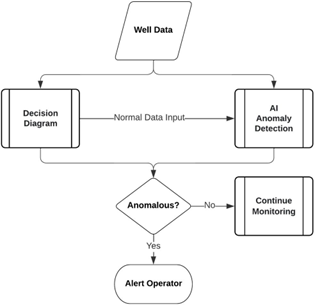
\includegraphics[width=0.55\textwidth]{DiagramaVIGIA2.png}
\caption{Fluxo geral do sistema dual. Os dados do poço alimentam simultaneamente o
diagrama de decisão e o módulo de detecção de anomalias por inteligência artificial. O
diagrama de decisão encaminha ao módulo de aprendizado apenas os trechos que classifica
como normais. Qualquer um dos dois componentes pode disparar o alerta ao operador.
Adaptado de \citet{aranha2023system}.}
\label{fig:dual-visaogeral}
\end{figure}

A \cref{fig:dual-visaogeral} mostra a estrutura. Note a seta rotulada como entrada de
dados normais: é ela que materializa a relação descrita acima. O autoencoder nunca vê
dados que o diagrama de decisão considera anômalos, e portanto o modelo de normalidade
que ele constrói não é contaminado por eventos.

\section{O diagrama de decisão}

O diagrama de decisão é uma árvore de regras organizada em quatro camadas sucessivas.
Cada camada responde a uma pergunta e restringe o espaço de hipóteses da seguinte.

\begin{figure}[htbp]
\centering
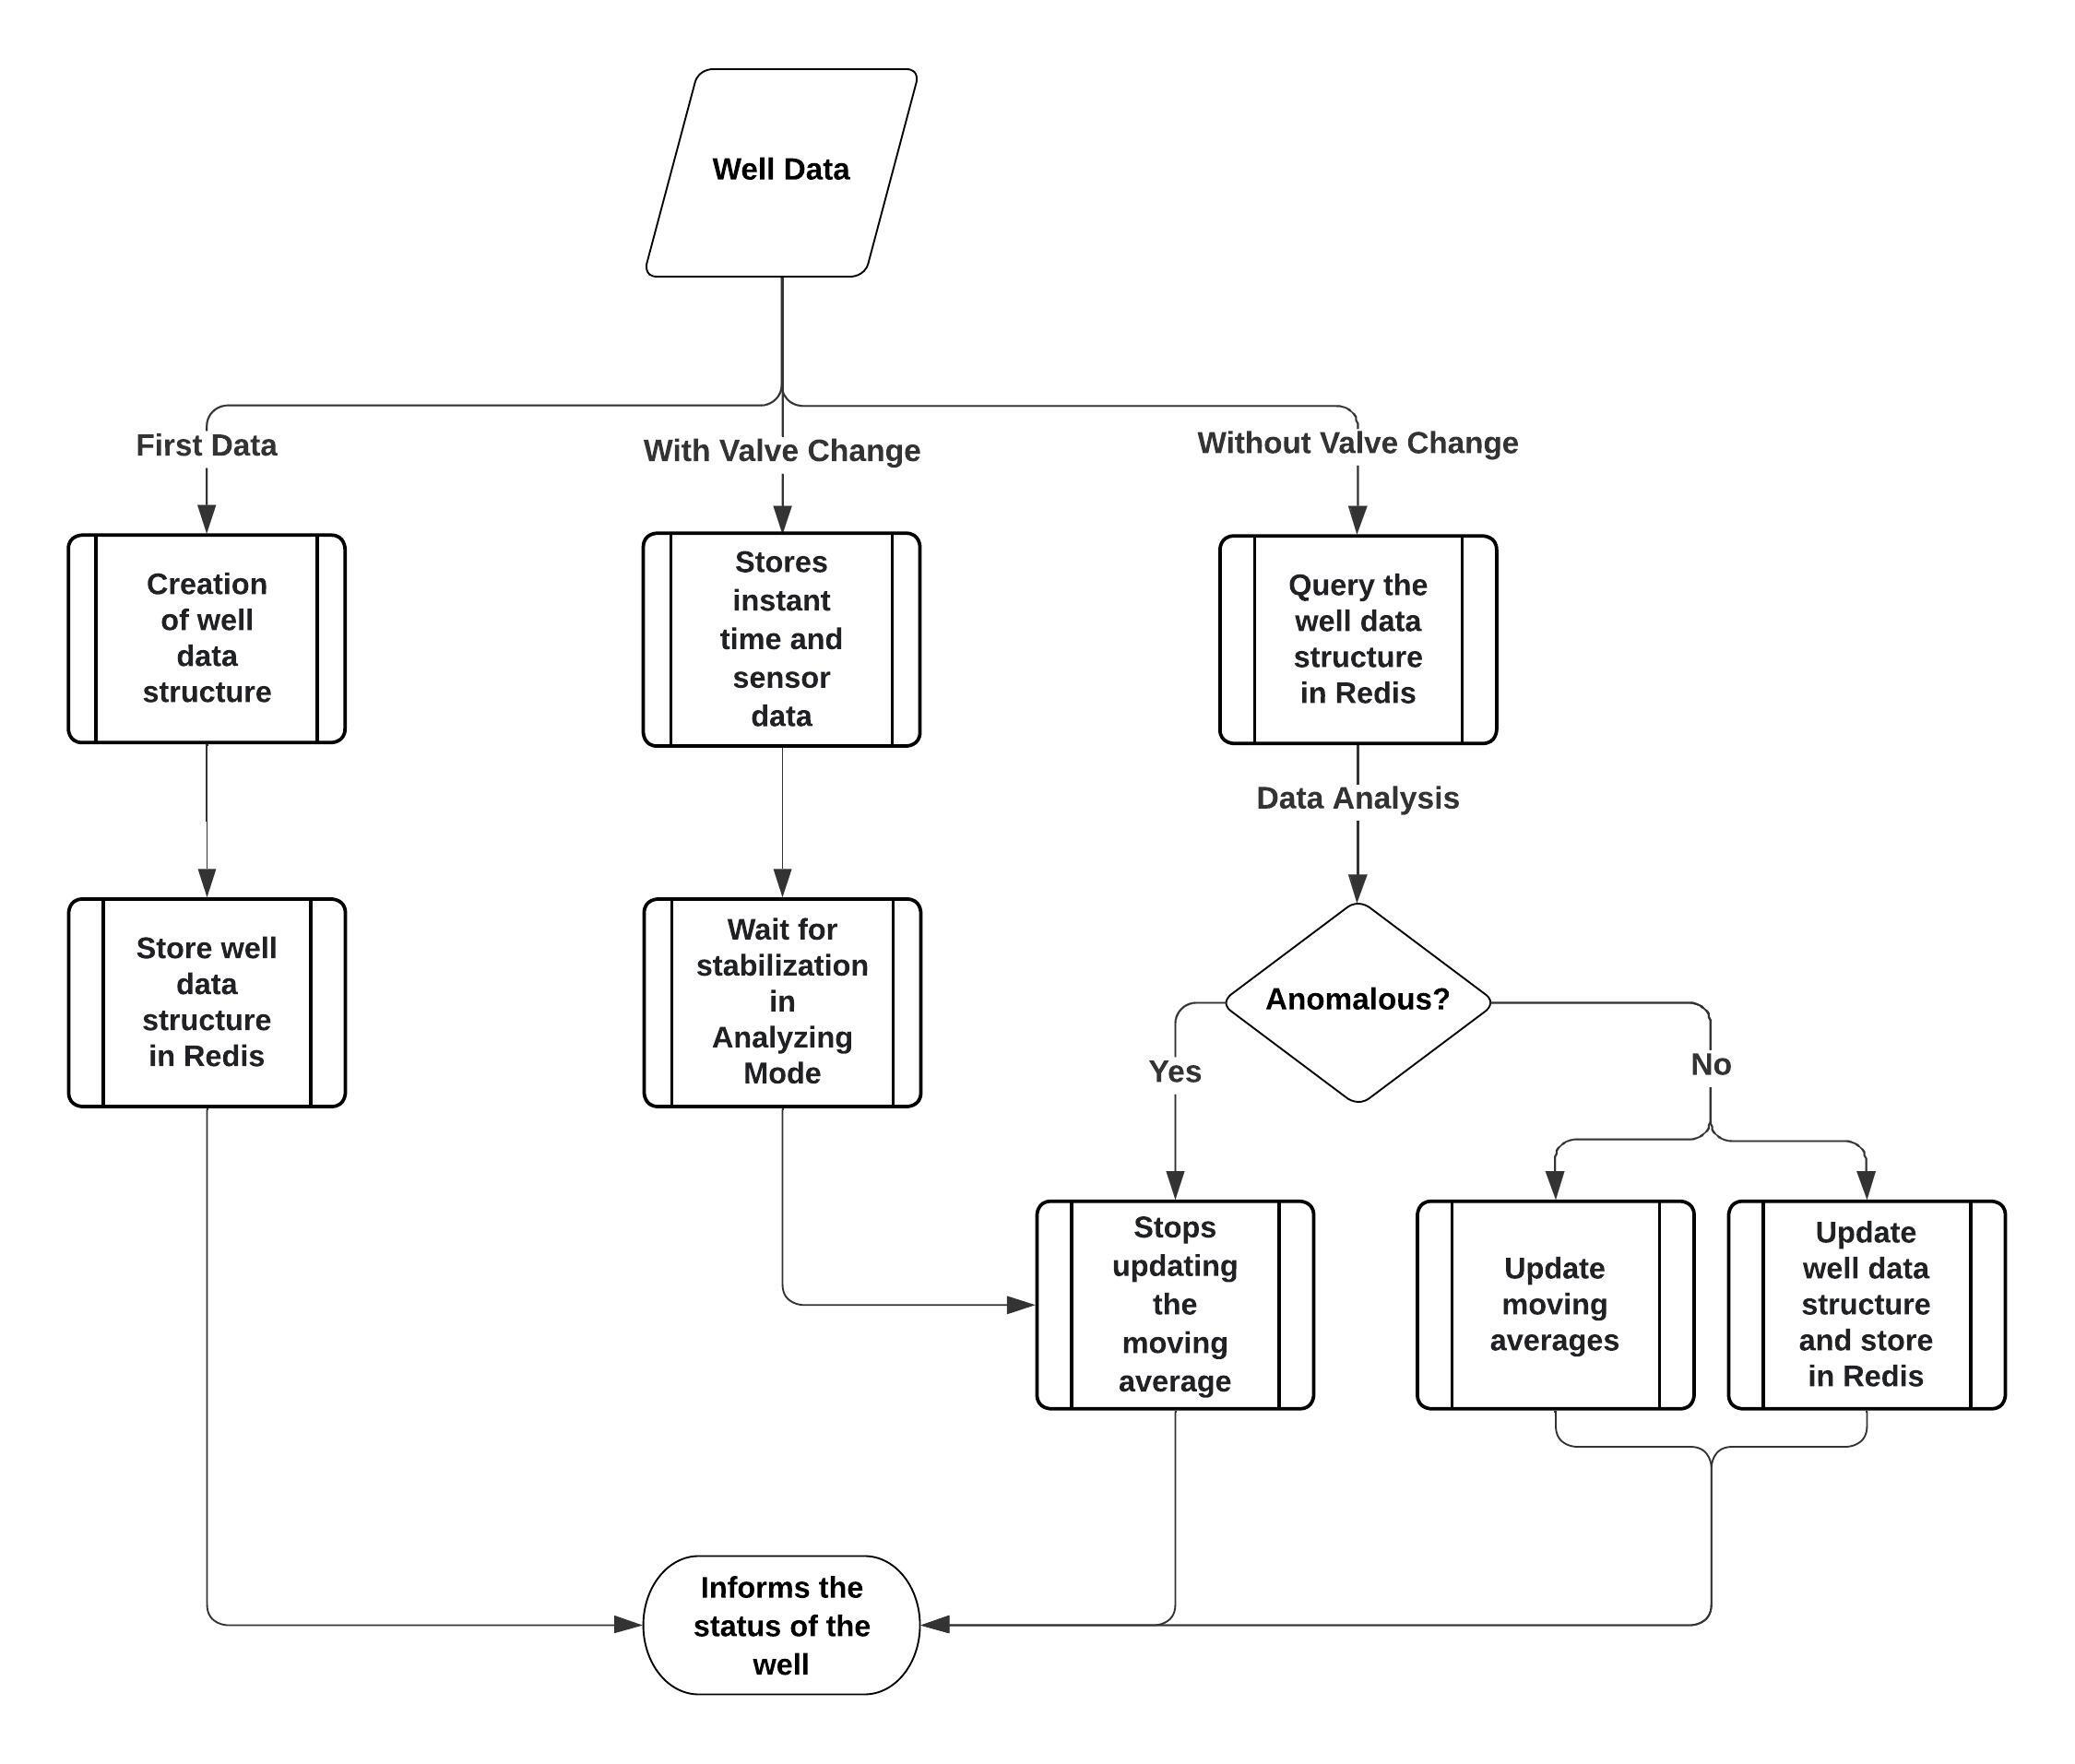
\includegraphics[width=0.9\textwidth]{New_Decision_Tree.jpeg}
\caption{Estrutura do diagrama de decisão. O fluxo bifurca conforme o dado seja o
primeiro do poço, siga uma mudança de estado de válvula ou dê continuidade a um regime já
estabelecido, encaminhando cada caso para estabilização, análise de anomalia ou
atualização da média móvel. Adaptado de \citet{aranha2023system}.}
\label{fig:dual-decisao}
\end{figure}

A \cref{fig:dual-decisao} mostra o fluxo. Vale insistir num ponto que a semelhança visual
esconde: apesar do nome e do formato, isto \emph{não} é uma árvore de decisão aprendida.
Nenhum de seus nós foi ajustado por otimização; cada bifurcação foi escrita por
engenheiros de produção e pode ser lida, auditada e alterada linha a linha. É conhecimento
declarado, não induzido --- e é essa diferença que sustenta a arquitetura dual descrita
neste capítulo.

\begin{enumerate}[leftmargin=*,itemsep=0.5em]

\item \textbf{Identificação do poço.} Qual poço é este, qual seu esquema de completação,
quais sensores estão disponíveis e quais são os limites operacionais declarados? Essa
camada não classifica nada --- ela carrega o contexto sem o qual as camadas seguintes
não podem operar. É também onde entram informações que nenhum modelo aprende dos dados:
profundidade, número de zonas produtoras, presença de gás de elevação.

\item \textbf{Tipo de dado.} O sinal recebido é válido? Esta camada implementa as
verificações discutidas no \cref{cap:dominio}: valor ausente, sensor congelado, leitura
fora da faixa física do instrumento, salto incompatível com a dinâmica do processo. Um
dado reprovado aqui não prossegue, e não contamina nem o alerta nem o treinamento.

\item \textbf{Transiente ou estabilizado?} O poço está em regime permanente ou em
transição? A distinção é essencial: durante uma partida, uma parada programada ou uma
manobra de válvula, os sinais apresentam variações de grande amplitude que são
perfeitamente normais. Sinalizá-las como anomalia é a receita para a fadiga de alarme
descrita no \cref{cap:introducao}.

\item \textbf{Análise de anomalia.} Somente aqui, com poço identificado, dado válido e
regime estabilizado, aplicam-se as regras de diagnóstico propriamente ditas ---
divergência entre pressões, queda de temperatura, oscilação sustentada.

\end{enumerate}

\begin{destaque}[Por que quatro camadas e não uma lista de regras]
A organização em camadas não é estética. Cada camada elimina uma fonte de falso
positivo antes que a próxima seja avaliada, e o resultado é que a última camada ---
a única que gera alarme --- opera sobre um subconjunto de dados já saneado. Uma lista
plana de regras avaliadas em paralelo produziria alarmes durante partidas, durante
falhas de sensor e durante manobras programadas.
\end{destaque}

\subsection{O tratamento de manobras de válvula}

Uma consequência prática merece destaque, porque é onde a maior parte dos sistemas
falha. Quando o operador altera deliberadamente o estado de uma válvula, o poço muda de
ponto de operação. Todos os sinais se deslocam. Um detector de anomalia baseado em
desvio da normalidade aprendida sinalizará --- corretamente, do ponto de vista
estatístico, e inutilmente, do ponto de vista operacional.

A solução adotada é radical e correta: \emph{ao detectar mudança de válvula, o sistema
descarta o modelo aprendido e reinicia o ciclo de treinamento}. O poço, depois da
manobra, é tratado como um poço novo. O custo é o período de reaprendizado; o benefício
é a ausência de alarmes espúrios sistemáticos.

\section{O detector por autoencoder}

\subsection{Lógica de operação}

\begin{figure}[htbp]
\centering
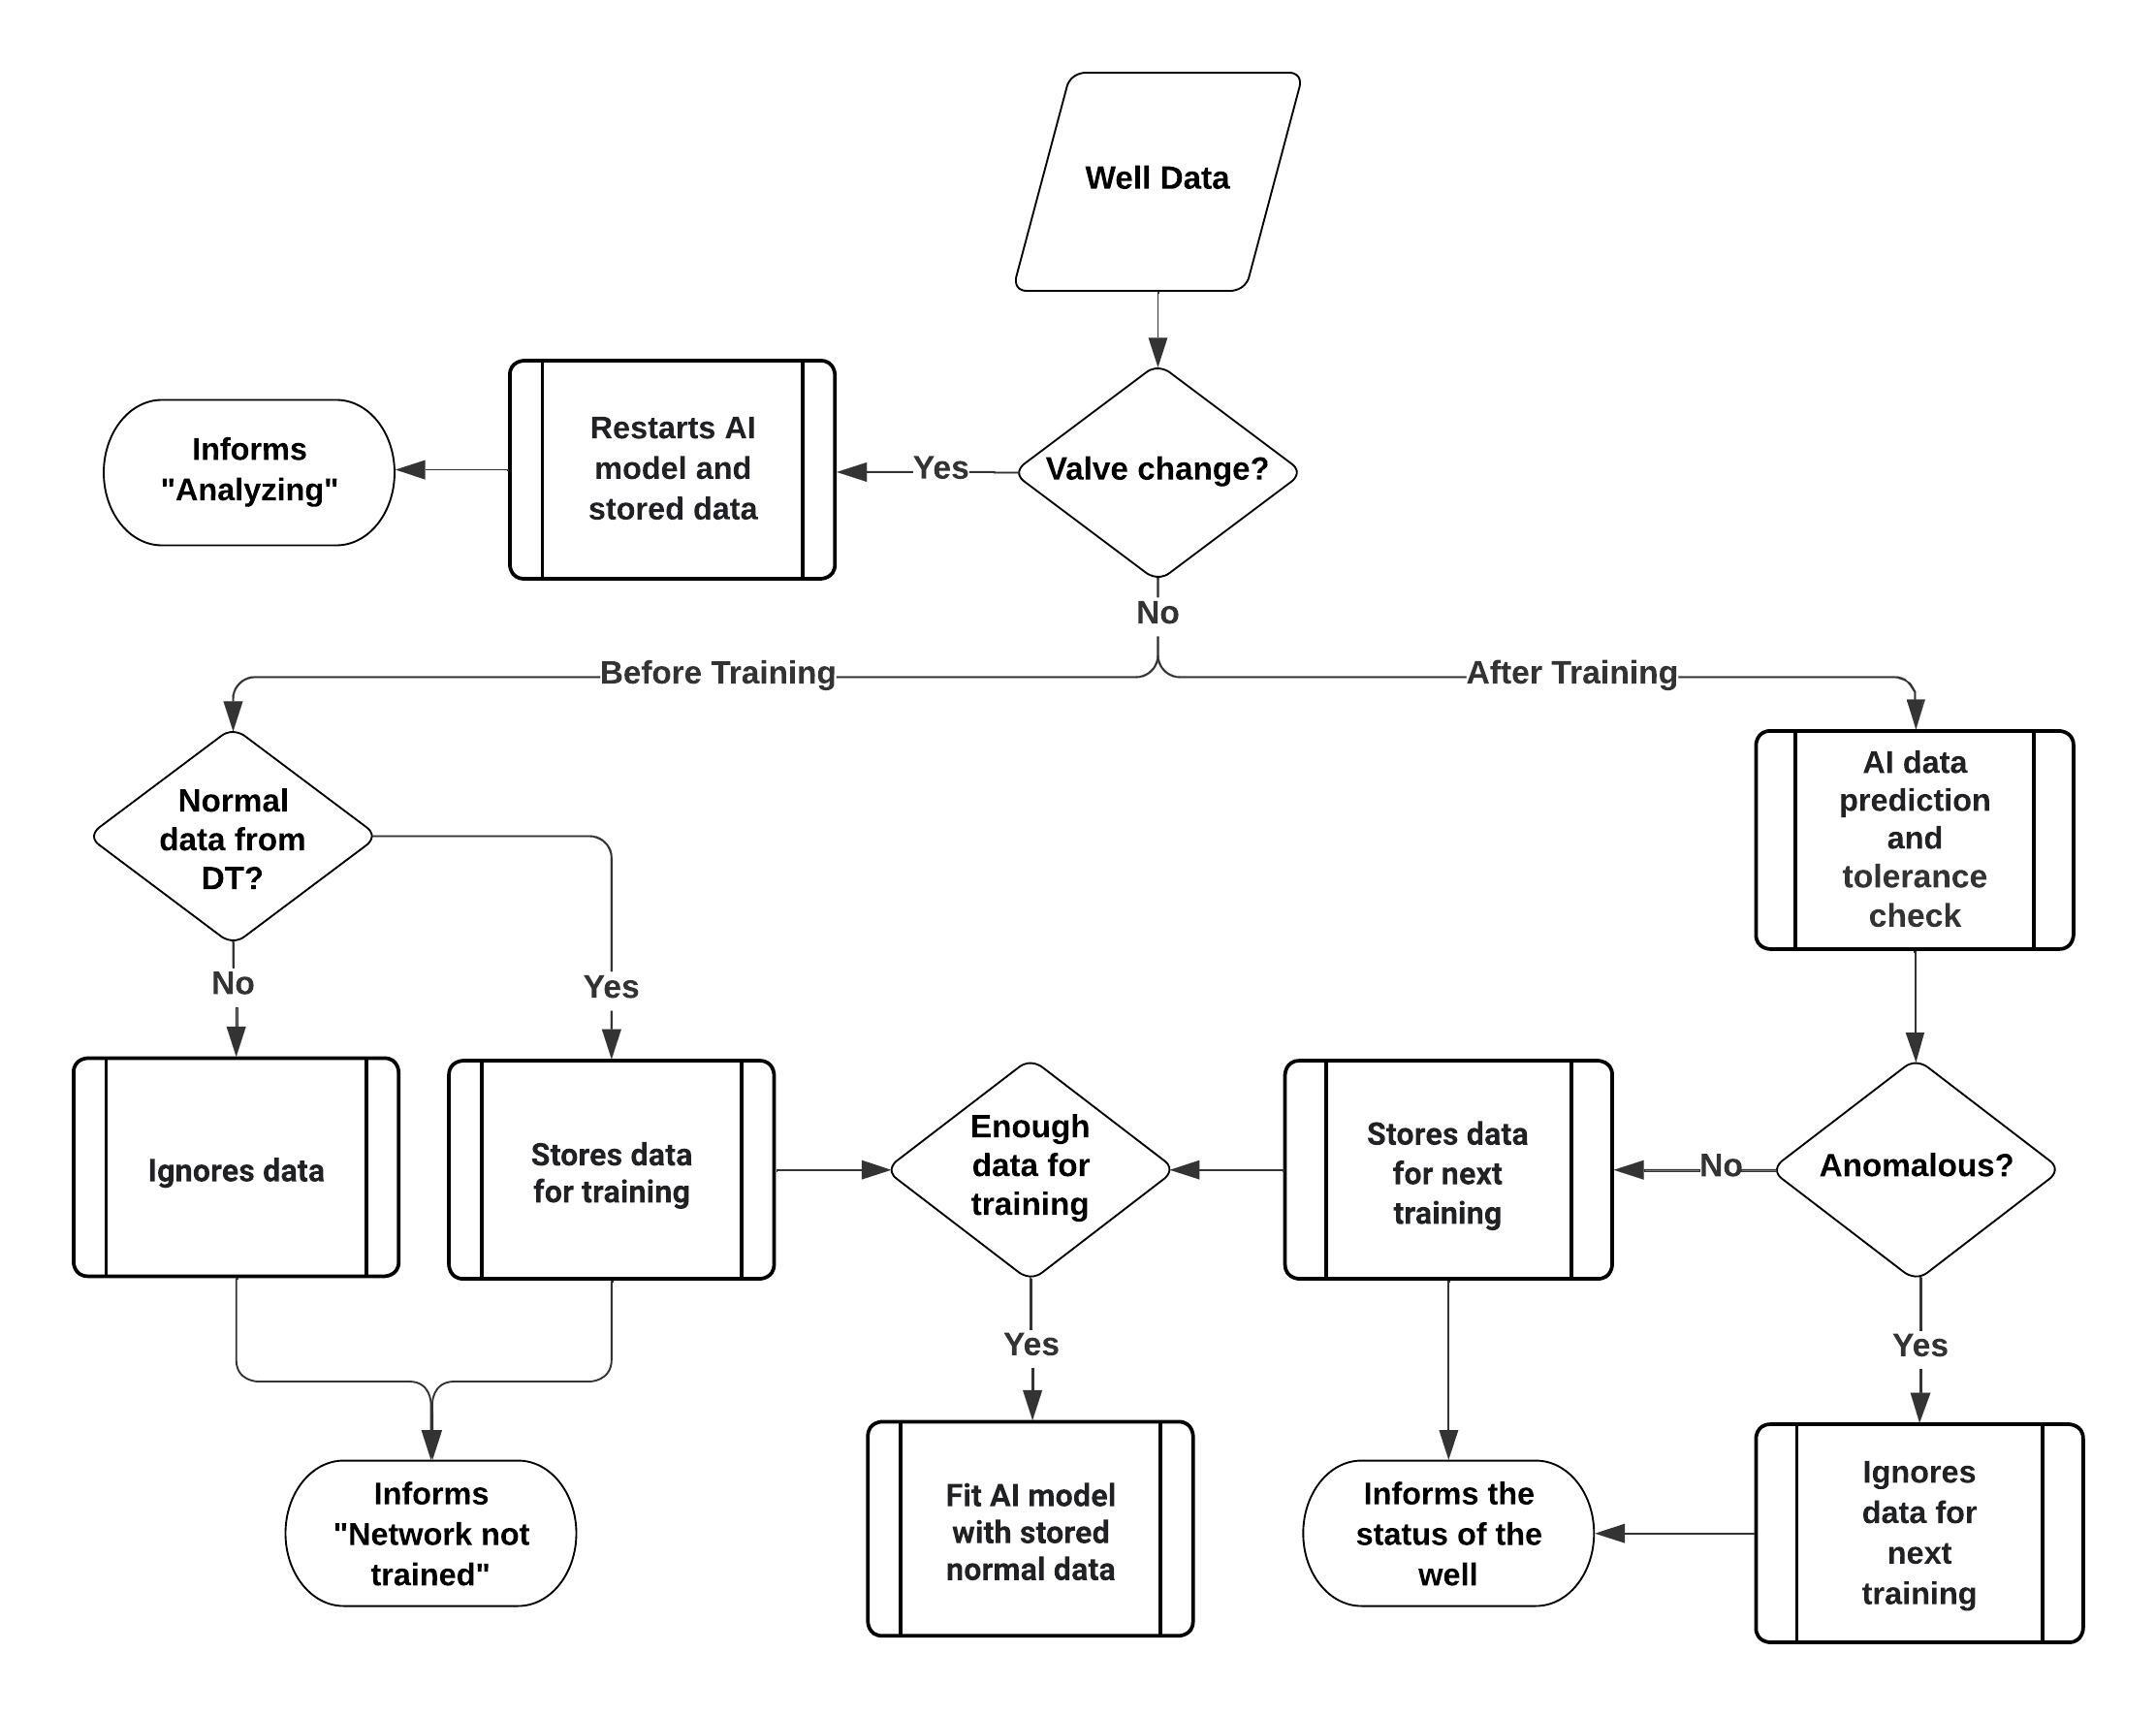
\includegraphics[width=\textwidth]{IA_flow_chart_2.jpeg}
\caption{Lógica operacional do módulo de detecção por inteligência artificial. Note os
três estados possíveis: antes do treinamento, o sistema apenas acumula dados normais
selecionados pelo diagrama de decisão; após o treinamento, ele prediz, compara com a
tolerância e informa o estado do poço; uma mudança de válvula reinicia o ciclo. Dados
julgados anômalos nunca retornam ao conjunto de treinamento. Adaptado de
\citet{aranha2023system}.}
\label{fig:dual-fluxo-ia}
\end{figure}

A \cref{fig:dual-fluxo-ia} detalha a máquina de estados. Três aspectos merecem
comentário.

\begin{itemize}[leftmargin=*,itemsep=0.4em]

\item \textbf{O sistema informa que não sabe.} Antes de acumular dados suficientes, ele
responde explicitamente ``rede não treinada''. Não há resposta silenciosamente errada.
É uma forma primitiva --- mas efetiva --- da rejeição que o \cref{cap:binarios}
formalizará.

\item \textbf{Dados anômalos são excluídos do treinamento futuro.} Sem essa
salvaguarda, o modelo aprenderia gradualmente a considerar a anomalia normal, e o
alarme se extinguiria sozinho. É a versão local do problema de deriva discutido no
\cref{cap:operacao}.

\item \textbf{O treinamento é contínuo.} Dados normais posteriores ao treinamento
inicial continuam sendo acumulados e usados em retreinamentos, o que permite ao modelo
acompanhar a evolução lenta e legítima do poço.

\end{itemize}

\subsection{Arquitetura da rede}

O autoencoder é do tipo \ing{sequence-to-sequence} com camadas LSTM. A entrada é um
tensor de forma $(\text{lote}, 500, 5)$: quinhentos passos de tempo de cinco sensores.

\begin{center}
\small
\begin{tabular}{lll}
\toprule
\textbf{Camada} & \textbf{Forma de saída} & \textbf{Função} \\
\midrule
Entrada                       & $(500, 5)$  & janela de \SI{500}{\second} \\
LSTM(16), ReLU                & $(500, 16)$ & codificação \\
LSTM(4), ReLU                 & $(4)$       & \textbf{representação latente} \\
\ing{RepeatVector}(500)       & $(500, 4)$  & replicação temporal \\
LSTM(16), ReLU                & $(500, 16)$ & decodificação \\
\ing{TimeDistributed} Densa(5)& $(500, 5)$  & reconstrução \\
\bottomrule
\end{tabular}
\end{center}

A compressão é de $500 \times 5 = \num{2500}$ valores para $4$: um fator de $625$. Essa
severidade é deliberada, e responde diretamente à advertência do \cref{cap:profundo}
sobre autoencoders excessivamente expressivos. Com quatro dimensões latentes, a rede não
tem como memorizar; ela é obrigada a capturar apenas a estrutura dominante da
normalidade.

\subsection{Treinamento}

\begin{center}
\small
\begin{tabular}{ll}
\toprule
\textbf{Hiperparâmetro} & \textbf{Valor} \\
\midrule
Função de perda      & SMAPE (\cref{eq:smape}) \\
Otimizador           & Adam \\
Épocas               & 500 \\
Tamanho do lote      & 100 \\
Ativação             & ReLU \\
Normalização         & Min-Max para $[0,1]$ \\
Ruído injetado       & 0 a 0,5\,\% \\
Dados mínimos        & $\approx 500$ amostras normais ($\approx \SI{5000}{\second}$) \\
\bottomrule
\end{tabular}
\end{center}

Duas escolhas merecem justificativa.

A \textbf{perda SMAPE} em vez do erro quadrático médio decorre da heterogeneidade de
escalas discutida no \cref{cap:aprendizado}: pressões da ordem de centenas de bar e
temperaturas da ordem de dezenas de graus. Um erro quadrático médio sobre variáveis
normalizadas ainda pondera implicitamente pela variância de cada canal; o SMAPE, sendo
relativo, trata todos os canais de forma comparável.

O \textbf{ruído injetado} de até 0,5\,\% cumpre dois papéis. Regulariza, impedindo que a
rede se apoie em detalhes de alta frequência específicos daquele poço; e simula a
variabilidade de instrumentação, tornando o modelo mais robusto quando transferido
entre poços com sensores de calibração ligeiramente diferente.

\subsection{Limiar e classificação de risco}

O escore de anomalia é o SMAPE de reconstrução. Sobre o conjunto de dados normais
acumulados, calculam-se $\mu$ e $\sigma$ desse escore, e define-se
\begin{equation}
  \tau = \mu + 3\sigma.
  \label{eq:dual-limiar}
\end{equation}

Sob normalidade aproximada, $\tau$ corresponde a aproximadamente $99{,}7\,\%$ dos casos
--- uma taxa nominal de falso positivo de $0{,}3\,\%$. A distribuição do erro de
reconstrução não é gaussiana, mas a regra é adequada como heurística e tem a virtude de
ser explicável a um operador em uma frase.

O valor do escore é então convertido em três níveis de risco:

\begin{figure}[htbp]
\centering
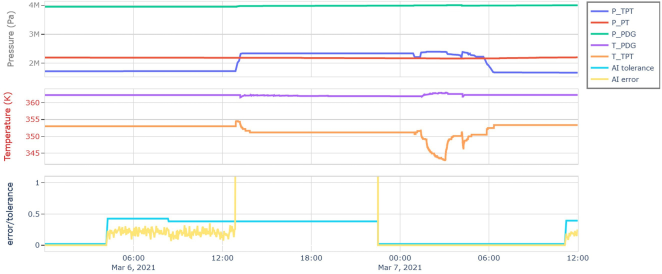
\includegraphics[width=0.86\textwidth]{abnormal.png}
\caption{Exemplo de detecção em dados reais. Nos dois painéis superiores, as pressões e
as temperaturas medidas por PDG e TPT; no inferior, o escore de anomalia com a linha de
tolerância da \cref{eq:dual-limiar}. A ultrapassagem do limiar precede em várias horas o
desvio que seria visível a olho nu nos sinais brutos. Adaptado de
\citet{aranha2023system}.}
\label{fig:dual-escore}
\end{figure}

\begin{center}
\small
\begin{tabular}{ll l}
\toprule
\textbf{Faixa} & \textbf{Nível} & \textbf{Ação recomendada} \\
\midrule
$< 30\,\%$          & Baixo & Registro; sem notificação. \\
$30\,\%$ a $70\,\%$ & Médio & Notificação ao operador; acompanhamento. \\
$> 70\,\%$          & Alto  & Alerta; investigação imediata. \\
\bottomrule
\end{tabular}
\end{center}

\begin{destaque}[Por que graduar o alarme]
Um alarme binário força uma escolha entre perder eventos e cansar o operador. A
graduação em três níveis desloca essa escolha para o operador, que dispõe de contexto
que o sistema não tem. É uma decisão de projeto de interface, não de aprendizado de
máquina, e é frequentemente o que separa um sistema usado de um sistema desligado.
\end{destaque}

\section{Implantação}

\begin{figure}[htbp]
\centering
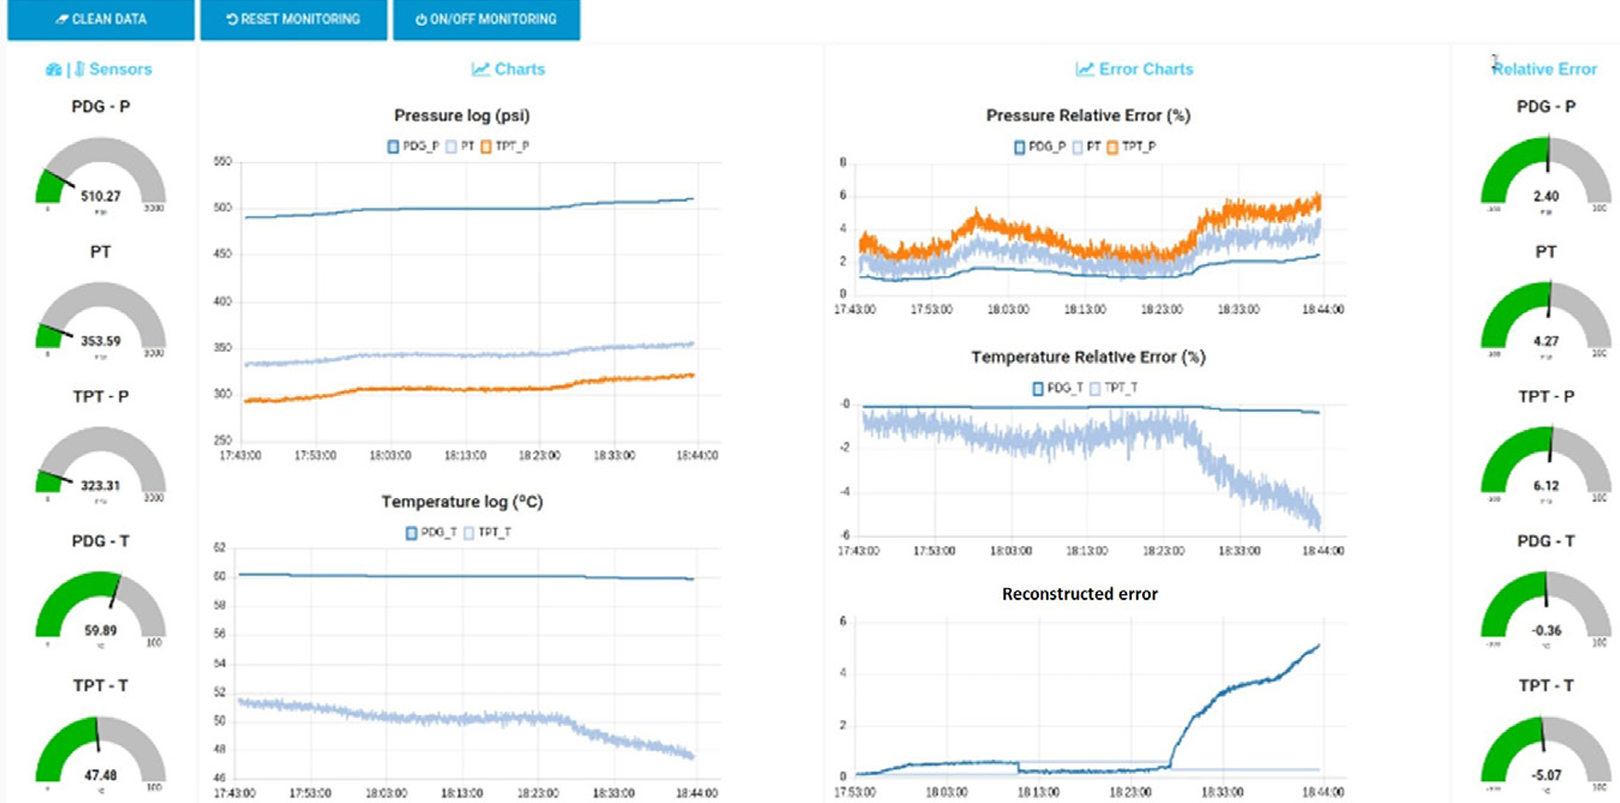
\includegraphics[width=\textwidth]{system.png}
\caption{Interface do sistema em operação. À esquerda, os valores instantâneos dos
cinco sensores monitorados; ao centro, os registros de pressão e temperatura; à
direita, os erros relativos de reconstrução por sensor e o erro agregado. O painel
inferior direito mostra o escore de anomalia cruzando o limiar, indicado pela linha
horizontal. Adaptado de \citet{aranha2023system}.}
\label{fig:dual-interface}
\end{figure}

O sistema foi implementado com Node-RED \citep{nodered} para orquestração de fluxo e
aquisição, e Python 3.7 com Keras \citep{Chollet2015} para o modelo. A escolha do
Node-RED merece nota: trata-se de uma ferramenta de programação visual por fluxo,
amplamente usada em automação industrial, que permite a engenheiros de operação
inspecionar e modificar o encadeamento sem tocar no código do modelo.

À época da avaliação reportada aqui, o sistema estava implantado em \textbf{mais de
vinte unidades flutuantes de produção} e \textbf{mais de duzentos e cinquenta poços
submarinos} nas bacias de Santos e de Campos.

\begin{destaque}[O que ``implantado'' significa]
Vale a pena explicitar, porque a palavra é usada com generosidade na literatura. Aqui
significa: executando continuamente em ambiente de produção da operadora, sobre dados
de tempo real, com saída visível a operadores em turno, e sujeito às consequências
operacionais de seus alertas. Não é um protótipo avaliado \ing{offline}.
\end{destaque}

\section{Resultados}
\label{sec:dual-resultados}

\subsection{Contribuição de cada componente}

A \cref{tab:dual-componentes} isola o efeito de acrescentar o autoencoder ao diagrama de
decisão.

\begin{table}[htbp]
\centering
\caption{Desempenho do diagrama de decisão isolado e do sistema dual completo.}
\label{tab:dual-componentes}
\begin{tabular}{lccc}
\toprule
\textbf{Configuração} & \textbf{ACC} & \textbf{ACC}$_b$ & $\bm{F_1}$ \\
\midrule
Diagrama de decisão                 & $0{,}9727$ & $0{,}9615$ & $0{,}9758$ \\
Diagrama de decisão + autoencoder   & $\bm{0{,}9894}$ & $\bm{0{,}9771}$ & $\bm{0{,}9917}$ \\
\bottomrule
\end{tabular}
\end{table}

\begin{resultadochave}
O acréscimo do autoencoder reduz o erro de $2{,}73\,\%$ para $1{,}06\,\%$ --- uma
redução relativa de aproximadamente $61\,\%$. A acurácia balanceada sobe de $0{,}9615$
para $0{,}9771$, e a medida $F_1$ de $0{,}9758$ para $0{,}9917$.
\end{resultadochave}

A leitura correta desse ganho exige cuidado. Em valor absoluto, $1{,}67$ ponto
percentual parece pouco. Em termos operacionais, significa que aproximadamente três em
cada cinco erros do sistema baseado em regras deixaram de ocorrer. Quando a base é um
sistema já bom, é assim que o progresso se manifesta.

\subsection{Comparação com a literatura}

O fechamento espúrio de DHSV (classe 2) é o evento mais estudado na literatura do 3W,
o que permite comparação direta.

\begin{table}[htbp]
\centering
\caption{Detecção de fechamento espúrio da DHSV: comparação com trabalhos anteriores.}
\label{tab:dual-literatura}
\begin{tabular}{llcc}
\toprule
\textbf{Trabalho} & \textbf{Método} & \textbf{ACC} & $\bm{F_1}$ \\
\midrule
\citet{Marins2021}  & Floresta aleatória      & $0{,}8708$ & --- \\
\citet{Turan2021}   & Árvore de decisão       & $0{,}6000$ & $0{,}4900$ \\
\citet{Machado2022} & LSTM                    & $\bm{0{,}9922}$ & $0{,}9360$ \\
Este capítulo       & Diagrama + autoencoder  & $0{,}9894$ & $\bm{0{,}9917}$ \\
\bottomrule
\end{tabular}
\end{table}

\begin{destaque}[Como ler esta tabela]
O sistema dual tem acurácia ligeiramente inferior à de \citet{Machado2022}
($0{,}9894$ contra $0{,}9922$) e medida $F_1$ substancialmente superior
($0{,}9917$ contra $0{,}9360$).

A combinação é diagnóstica. Uma medida $F_1$ de $0{,}9360$ com acurácia de $0{,}9922$
indica desequilíbrio entre precisão e revocação --- tipicamente, muitos falsos
positivos ou muitos falsos negativos concentrados na classe minoritária, mascarados
pela acurácia global (\cref{cap:aprendizado}). O sistema dual apresenta as duas métricas
alinhadas, o que indica desempenho equilibrado.

Uma ressalva de honestidade: os conjuntos de avaliação não são idênticos entre os
trabalhos, e a comparação é indicativa, não conclusiva.
\end{destaque}

\subsection{Estudos de caso em poços reais}

Os três casos a seguir são eventos reais, com data e hora, detectados pelo sistema em
operação. Eles importam porque são a única evidência disponível sobre generalização a
condições que nenhum conjunto de dados público contém.

\begin{table}[htbp]
\centering
\caption{Estudos de caso: características dos poços. WD é a lâmina d'água e TD a
profundidade total.}
\label{tab:dual-pocos}
\small
\begin{tabular}{lllll}
\toprule
\textbf{Poço} & \textbf{Tipo} & \textbf{WD (m)} & \textbf{TD (m)} & \textbf{Zonas} \\
\midrule
1 & Produtor, pré-sal de Santos & \num{2041} & \num{5870} & 3 (\num{5432} a \num{5774}\,m) \\
2 & Produtor                    & \num{2125} & \num{5552} & 2 (\num{5137} a \num{5440}\,m) \\
3 & Injetor WAG                 & \num{1946} & \num{6197} & 3 (\num{5437} a \num{5730}\,m) \\
\bottomrule
\end{tabular}
\end{table}

\begin{table}[htbp]
\centering
\caption{Estudos de caso: eventos detectados e desempenho. O SMAPE indicado é o valor de
pico do erro de reconstrução durante o evento.}
\label{tab:dual-casos}
\small
\begin{tabular}{llcccc}
\toprule
\textbf{Poço} & \textbf{Evento} & \textbf{Data e hora} & \textbf{SMAPE} &
\textbf{ACC}$_b$ & $\bm{F_1}$ \\
\midrule
1 & Fechamento espúrio (1º) & 01/08/2022 01:16 & $39{,}148\,\%$ & $0{,}9897$ & $0{,}9987$ \\
1 & Fechamento espúrio (2º) & 01/08/2022 08:48 & $48{,}312\,\%$ & $0{,}9988$ & $0{,}9989$ \\
2 & Comunicação de pressão na CKGL & 06/06/2018 14:37 & $33{,}136\,\%$ & $0{,}9998$ & $0{,}9998$ \\
3 & Fechamento espúrio DHSV/M1 & 18/10/2022 02:10 & $23{,}390\,\%$ & $0{,}9988$ & $0{,}9991$ \\
\bottomrule
\end{tabular}
\end{table}

\begin{figure}[htbp]
\centering
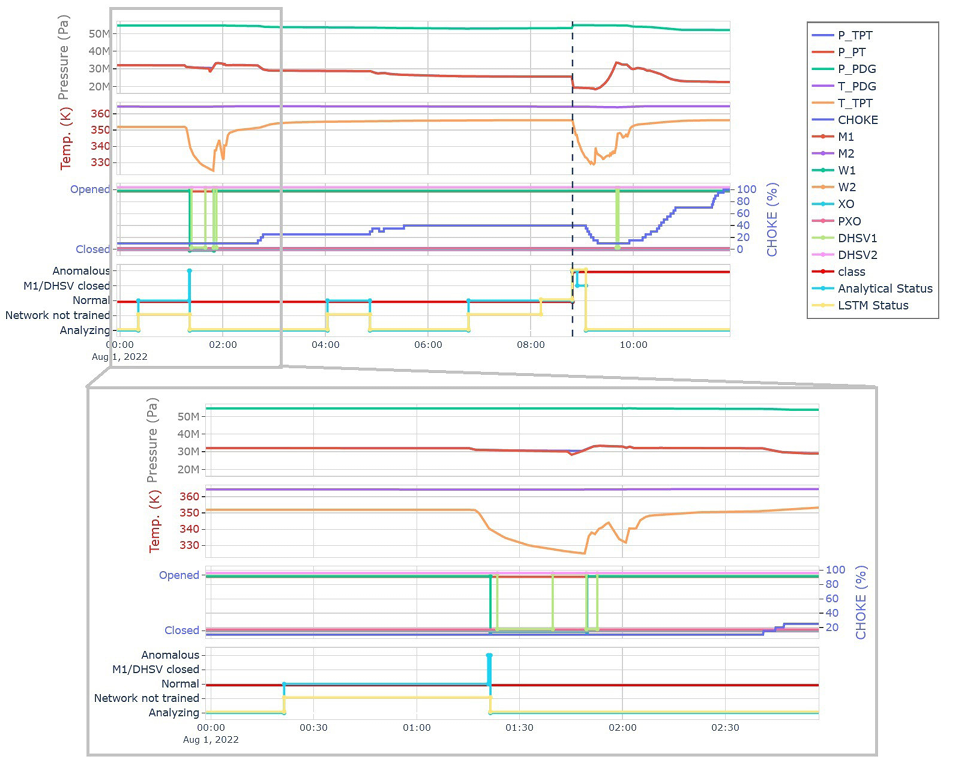
\includegraphics[width=\textwidth]{fig8.png}
\caption{Poço 1, primeiro evento. De cima para baixo: os sensores PDG, PT e TPT, o estado
das válvulas e a comparação entre a classificação dos dois modelos (\emph{LSTM status} e
\emph{analytical status}) e a classificação humana posterior (\emph{class}). Adaptado de
\citet{aranha2023system}.}
\label{fig:dual-poco1a}
\end{figure}

\begin{figure}[htbp]
\centering
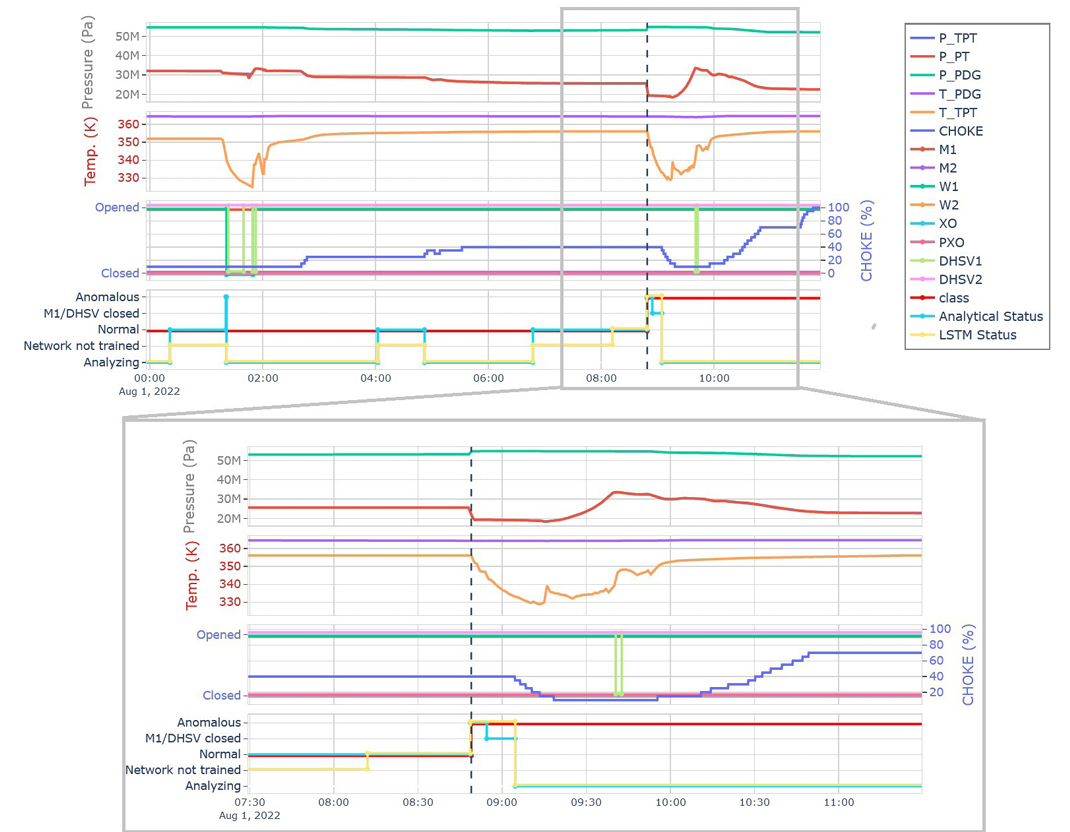
\includegraphics[width=\textwidth]{fig9.png}
\caption{Poço 1, segundo evento, no mesmo dia. Adaptado de \citet{aranha2023system}.}
\label{fig:dual-poco1b}
\end{figure}

A \cref{fig:dual-poco1a,fig:dual-poco1b} apresentam os dois eventos do poço 1, e a
comparação entre elas contém a lição mais útil do capítulo sobre a divisão de trabalho
entre as duas camadas.

No primeiro evento, às 01:16, \textbf{apenas o diagrama analítico detectou}. A rede não
teve chance: o fechamento espúrio da DHSV alterou o estado das válvulas, e o sistema
entrou em modo de análise --- justamente o comportamento projetado para evitar alarmes
durante manobras. O operador corrigiu com ciclagem de válvulas entre 01:39 e 01:52.

No segundo evento, às 08:48, \textbf{ambos detectaram}, e o diagrama classificou
corretamente a causa como fechamento espúrio da DHSV ou da M1.

\begin{destaque}[Por que isto justifica a arquitetura dual]
O primeiro evento é o argumento inteiro deste capítulo em uma linha: houve uma anomalia
real que a rede neural, por construção, não podia enxergar. A regra explícita enxergou.

Um sistema apenas aprendido teria perdido esse evento. Um sistema apenas analítico teria
perdido a classificação mais fina que a rede oferece em outros casos. A redundância não
é conservadorismo --- é a única configuração em que a janela cega de um componente é
coberta pelo outro.
\end{destaque}

\begin{figure}[htbp]
\centering
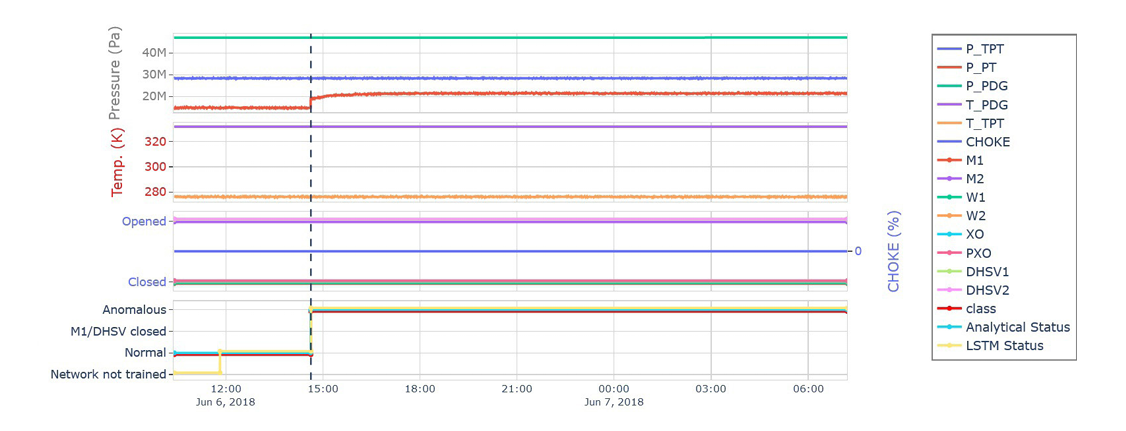
\includegraphics[width=\textwidth]{fig10.png}
\caption{Poço 2, retroanálise do evento de 6 de junho de 2018. Adaptado de
\citet{aranha2023system}.}
\label{fig:dual-poco2}
\end{figure}

\begin{figure}[htbp]
\centering
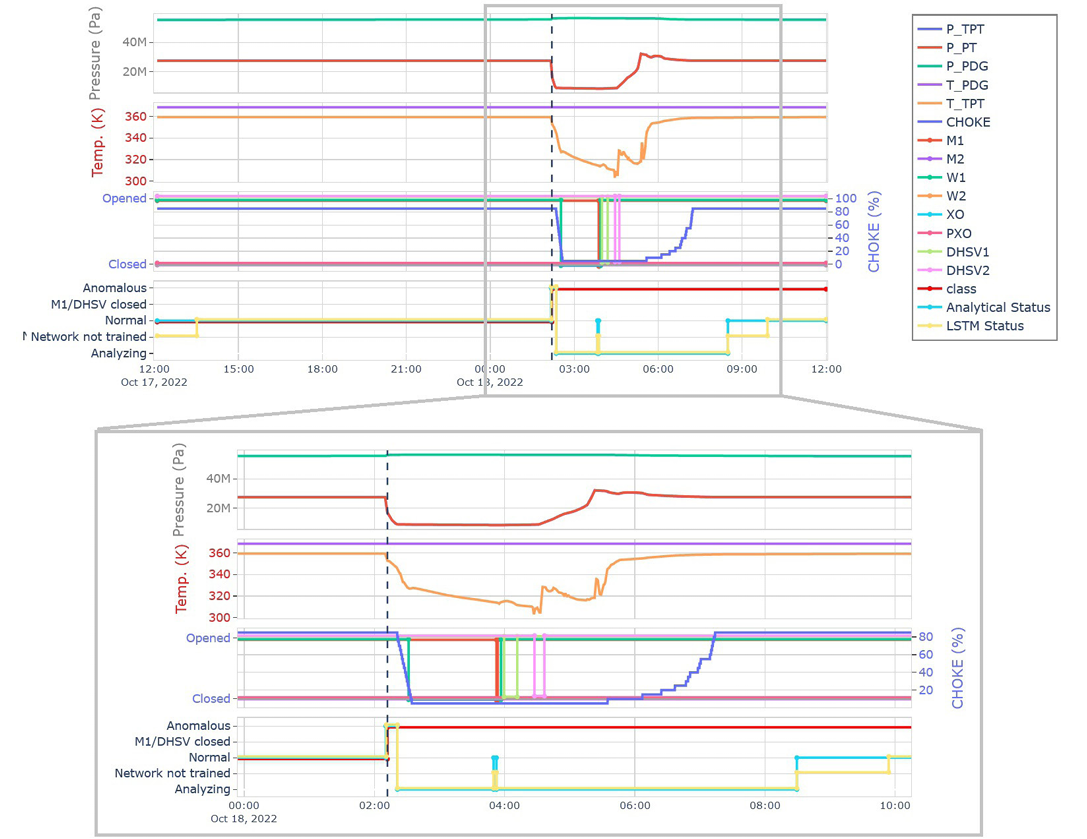
\includegraphics[width=\textwidth]{fig11.png}
\caption{Poço 3, evento de 18 de outubro de 2022, com o ciclo completo: detecção,
fechamento pelo operador, ciclagem, reabertura e retorno à normalidade. Adaptado de
\citet{aranha2023system}.}
\label{fig:dual-poco3}
\end{figure}

\begin{exemplo}{O poço 3, minuto a minuto}
O caso do poço 3, mostrado na \cref{fig:dual-poco3}, é o mais instrutivo, porque tem
começo, meio e fim documentados.

Trata-se de um injetor de água e gás alternados (WAG) em lâmina d'água de
\SI{1946}{\meter}. Às \textbf{02:10} de 18 de outubro de 2022, DHSV e M1 fecharam sem
comando. O sistema sinalizou o desvio com SMAPE de pico de $23{,}390\,\%$. As válvulas
foram reabertas às \textbf{07:14}, e o poço retornou à condição normal às
\textbf{08:29}.

Dois pontos merecem atenção. Primeiro, o SMAPE de pico deste caso é o menor dos quatro
--- cerca de metade do observado no segundo evento do poço 1 --- e ainda assim
suficiente para ultrapassar o limiar com folga. Isso indica que $\tau = \mu + 3\sigma$
está calibrado de forma conservadora o bastante para eventos de assinatura mais
discreta.

Segundo, o sistema acompanhou corretamente o \emph{retorno} à normalidade, com uma hora
e quinze minutos de defasagem em relação à reabertura das válvulas --- o tempo físico
de reestabilização do poço, não um atraso do algoritmo.
\end{exemplo}

\begin{exemplo}{O poço 2 e o valor de detectar o não catalogado}
O evento do poço 2 foi uma comunicação indevida de pressão através da válvula
reguladora de gás de elevação. \emph{Esse evento não pertence a nenhuma das nove classes
do 3W}, não estava programado no diagrama de decisão e não teria sido detectado por
nenhum classificador supervisionado treinado no catálogo padrão.

Foi detectado pelo autoencoder, com $\text{ACC}_b = 0{,}9998$, simplesmente porque não
se parecia com a normalidade daquele poço. A \cref{fig:dual-poco2} mostra a retroanálise:
o desvio é visível nos três sensores muito antes de a intervenção ter sido decidida em
campo.

É a demonstração mais direta do argumento deste livro: o componente que não sabe o nome
de nada é o único capaz de reagir ao que ainda não tem nome. O que lhe falta ---
dizer \emph{o que} está acontecendo --- é o que os \cref{cap:binarios,cap:mundoaberto}
e, em outro registro, a \cref{parte:explicabilidade} vão perseguir.
\end{exemplo}

\section{Limitações}

\begin{enumerate}[leftmargin=*,itemsep=0.4em]

\item \textbf{Não classifica.} O autoencoder responde ``anômalo'' ou ``normal''. O
diagrama de decisão classifica, mas apenas o que foi programado. Nenhum dos dois nomeia
um evento inédito.

\item \textbf{Período cego.} São necessárias aproximadamente quinhentas amostras normais
--- cerca de uma hora e vinte e três minutos --- antes que o modelo esteja disponível. E
o relógio reinicia a cada mudança de válvula.

\item \textbf{Limiar único e global.} Um único $\tau$ para todos os sensores e todos os
regimes. Um evento que afete fortemente um sensor e pouco os demais pode ser diluído no
erro agregado.

\item \textbf{Hipótese de normalidade sobre o erro.} A regra $\mu + 3\sigma$ pressupõe
uma distribuição que os dados não seguem exatamente. Na prática funciona, mas a taxa de
falso positivo nominal de $0{,}3\,\%$ não deve ser levada ao pé da letra.

\item \textbf{Avaliação limitada.} Três poços e quatro eventos. É evidência forte de
funcionamento e evidência fraca de generalização.

\end{enumerate}

\begin{destaque}[Para onde isso leva]
A limitação (1) é a mais estrutural, e é ela que abre o \cref{cap:binarios}: como
transformar ``algo está errado'' em ``isto é um hidrato'' \emph{sem} recair na hipótese
de mundo fechado que o \cref{cap:introducao} descartou.
\end{destaque}

\resumocapitulo{%
O sistema dual combina um diagrama de decisão determinístico em quatro camadas ---
identificação do poço, validação do dado, discriminação de transiente e análise de
anomalia --- com um autoencoder LSTM que comprime janelas de quinhentos segundos e cinco
sensores em quatro dimensões latentes. A relação entre os componentes é de mão dupla: o
diagrama seleciona os dados normais que treinam o autoencoder, e o autoencoder cobre os
eventos que o diagrama não enumera. O limiar de detecção é $\mu + 3\sigma$ sobre o SMAPE
de reconstrução, convertido em três níveis de risco. O sistema opera em mais de vinte
unidades flutuantes e mais de duzentos e cinquenta poços. O acréscimo do autoencoder ao
diagrama eleva a acurácia de $0{,}9727$ para $0{,}9894$ e a medida $F_1$ de $0{,}9758$
para $0{,}9917$, resultado competitivo com o estado da arte na detecção de fechamento
espúrio de DHSV. Quatro eventos reais em três poços confirmam o funcionamento em campo,
inclusive para um evento fora do catálogo. A limitação decisiva é que o sistema detecta
sem classificar --- e é essa lacuna que o restante da Parte II ataca.}

\begin{exercicios}
\item O autoencoder comprime $500 \times 5 = \num{2500}$ valores em quatro dimensões.
      Calcule a taxa de compressão e discuta, em termos de teoria da informação, que
      tipos de estrutura podem sobreviver a essa compressão e quais necessariamente se
      perdem.

\item Implemente o autoencoder descrito neste capítulo e treine-o sobre instâncias
      normais do 3W. Compare o histograma do SMAPE de reconstrução em dados normais e
      anômalos e verifique empiricamente se $\mu + 3\sigma$ é uma escolha adequada de
      limiar. Teste também $\mu + 2\sigma$ e $\mu + 4\sigma$, reportando a curva ROC.

\item O sistema reinicia o treinamento a cada mudança de válvula. Modele o custo dessa
      política: dado um poço com $\lambda$ manobras por mês e um período cego de
      \SI{5000}{\second}, qual a fração de tempo em que o sistema está indisponível?
      Para que valor de $\lambda$ a indisponibilidade ultrapassa $10\,\%$?

\item Proponha e justifique uma alternativa ao reinício completo após manobra de
      válvula. Considere: um modelo por estado de válvula; um modelo condicionado ao
      estado como entrada adicional; adaptação incremental. Discuta prós e contras.

\item O sistema usa um limiar único sobre o erro agregado. Proponha um esquema de
      limiares por sensor e discuta como combinar as decisões individuais. Que ganho
      você esperaria para um evento que afeta apenas a temperatura de fundo?

\item A \cref{tab:dual-literatura} mostra $\text{ACC} = 0{,}9922$ com $F_1 = 0{,}9360$
      para um dos trabalhos. Construa uma matriz de confusão compatível com esse par de
      valores e explique qual desequilíbrio ele revela.

\item Discuta criticamente a evidência dos estudos de caso. Quatro eventos em três poços
      sustentam qual afirmação? Formule três afirmações de força decrescente e indique
      qual delas os dados suportam.
\end{exercicios}

\begin{leituras}
\item \citet{LopesTese2025} --- a tese que originou este capítulo, com detalhamento
      adicional do diagrama de decisão.
\item \citet{Machado2022}, \citet{Marins2021} e \citet{Turan2021} --- os trabalhos
      comparados na \cref{tab:dual-literatura}.
\item \citet{aranha2023system} e \citet{Aranha2024} --- descrição de sistemas de
      monitoramento em operação, com os requisitos de campo que motivaram a arquitetura
      dual.
\item \citet{Malhotra2015LongST} --- referência clássica sobre autoencoders LSTM para
      detecção de anomalias em séries temporais.
\end{leituras}

\chapter{Ensemble de classificadores binários}
\label{cap:binarios}

\begin{objetivos}
Ao final deste capítulo, você será capaz de:
\begin{itemize}[leftmargin=*,itemsep=0.2em]
  \item explicar a diferença estrutural entre um classificador multiclasse e um ensemble
        de classificadores binários um-contra-todos, e por que apenas o segundo pode
        expressar rejeição;
  \item projetar e treinar um classificador binário por classe de anomalia, incluindo o
        tratamento do desbalanceamento da classe negativa;
  \item conduzir uma busca sistemática de hiperparâmetros e interpretar seus resultados;
  \item comparar o desempenho por classe do ensemble binário com o de um classificador
        multiclasse, de uma OCSVM e da literatura;
  \item reconhecer as classes em que a abordagem falha e formular hipóteses sobre o
        motivo.
\end{itemize}
\end{objetivos}

\section{Uma mudança de pergunta}

O \cref{cap:dual} terminou com um sistema que detecta sem classificar. A tentação
natural é acoplar-lhe um classificador multiclasse: nove classes, uma camada
\ing{softmax}, entropia cruzada categórica. É a solução que qualquer curso introdutório
sugeriria, e é a solução que o \cref{cap:introducao} descartou.

Este capítulo desenvolve a alternativa. Em vez de perguntar

\begin{center}
\emph{``qual das nove classes é esta janela?''}
\end{center}

\noindent
pergunta-se, nove vezes de forma independente,

\begin{center}
\emph{``esta janela é da classe $k$? Sim ou não.''}
\end{center}

\begin{destaque}[Por que isso não é uma reformulação vazia]
Em mundo fechado, as duas formulações são equivalentes: dado que a janela pertence a
alguma das nove classes, saber a resposta das nove perguntas binárias é saber a resposta
da pergunta multiclasse.

Em mundo aberto, elas deixam de ser equivalentes, e a razão é puramente estrutural.
O classificador multiclasse produz escores acoplados pela restrição
$\sum_k \hat{p}_k = 1$: se um escore cai, outro necessariamente sobe. Os nove
classificadores binários produzem escores \emph{independentes}, cada um saído de sua
própria sigmoide. Nada os impede de serem todos simultaneamente baixos --- e
``todos baixos'' é a assinatura do desconhecido.
\end{destaque}

Formalmente, a regra de decisão é a \cref{eq:ensemble-rejeicao} do \cref{cap:novidades}:
\[
  \hat{y} = \begin{cases}
    \argmax_{k} s_k(\mat{X}), & \text{se } \max_k s_k(\mat{X}) > \tau, \\[0.3em]
    \texttt{desconhecido},    & \text{caso contrário.}
  \end{cases}
\]

\subsection{Três consequências adicionais}

A independência dos classificadores traz três benefícios que não são o objetivo
declarado, mas que se revelaram decisivos.

\begin{description}[leftmargin=0pt,style=nextline,itemsep=0.5em]

\item[Extensibilidade incremental.] Acrescentar uma décima classe custa \emph{um}
treinamento. Nenhum dos nove classificadores existentes precisa ser tocado, porque
nenhum deles depende dos demais. Em um classificador multiclasse, acrescentar uma classe
altera a camada de saída e exige retreinamento completo. Essa propriedade é o que torna
viável o ciclo de incorporação de novas classes do \cref{cap:mundoaberto}.

\item[Otimização independente.] Cada classe pode ter sua própria arquitetura, seu
próprio comprimento de janela, seu próprio limiar. Um evento lento como a incrustação
(classe 7) e um evento abrupto como o fechamento de DHSV (classe 2) não precisam
compartilhar hiperparâmetros --- e, como argumentou o \cref{cap:dominio}, eles não
deveriam.

\item[Diagnóstico interpretável.] Quando o sistema erra, sabe-se \emph{qual} dos nove
classificadores errou. Em um classificador multiclasse, o erro é uma propriedade do
modelo inteiro.

\end{description}

\subsection{E os custos}

Três, e vale enunciá-los com a mesma clareza.

Primeiro, \textbf{custo computacional multiplicado por nove} --- quantificado no
\cref{cap:closedworld} e, como se verá, irrelevante na prática. Segundo,
\textbf{possibilidade de conflito}: dois classificadores podem reivindicar a mesma
janela com escores altos, situação que a regra $\argmax$ resolve arbitrariamente e que
o \cref{cap:mundoaberto} tratará com voto ponderado. Terceiro, \textbf{desbalanceamento
severo em cada tarefa binária}: ao treinar o classificador da classe $k$, todas as
demais classes formam a classe negativa, tipicamente numa razão de oito ou nove para
um.

\section{Metodologia}

\begin{figure}[htbp]
\centering
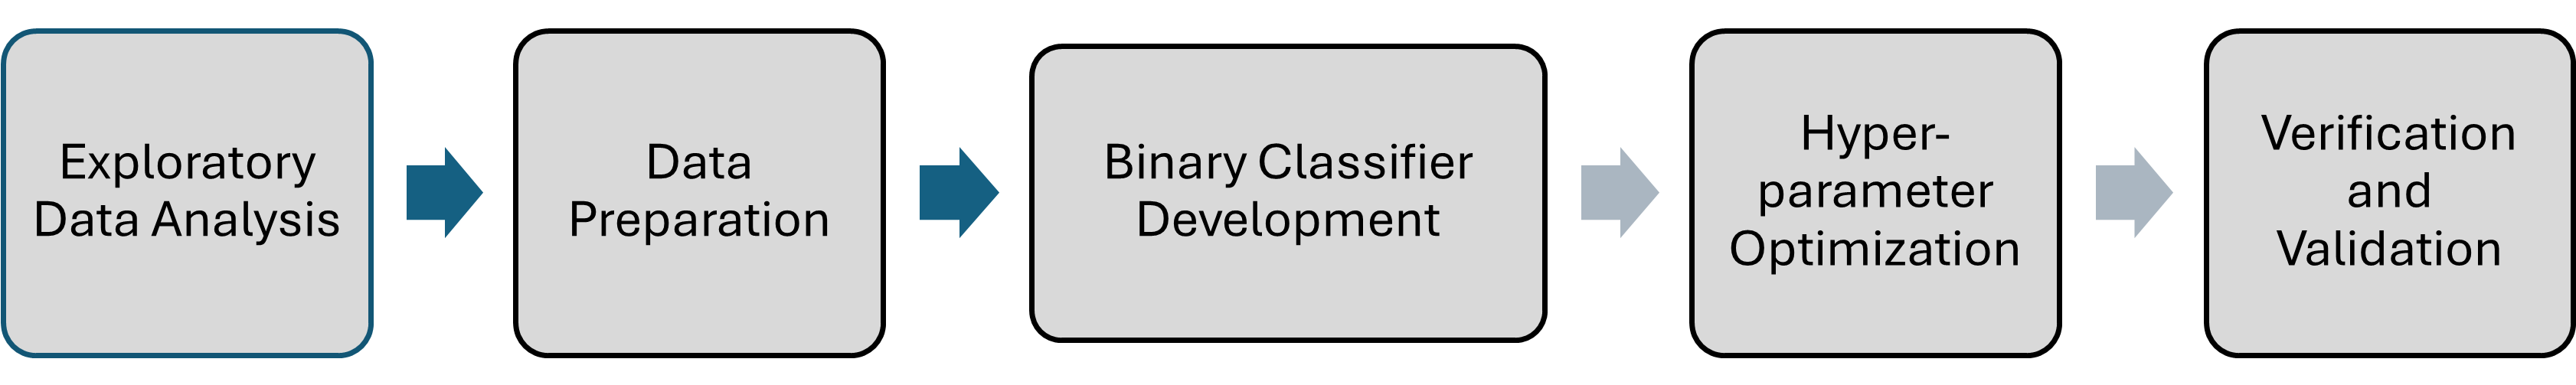
\includegraphics[width=\textwidth]{binary_diagram.png}
\caption{Fluxo metodológico do desenvolvimento dos classificadores binários: análise
exploratória, preparação dos dados, construção dos classificadores, otimização de
hiperparâmetros e, por fim, verificação e validação --- esta última incluindo a
comparação com um modelo termodinâmico independente, discutida no
\cref{cap:closedworld}.}
\label{fig:binarios-fluxo}
\end{figure}

\subsection{Análise exploratória}

A etapa que costuma ser omitida em artigos é aqui a que determina as decisões seguintes.
Três achados orientaram o projeto.

\begin{enumerate}[leftmargin=*,itemsep=0.4em]

\item \textbf{Forte correlação entre sensores.} As pressões de fundo e de cabeça são
altamente correlacionadas em regime normal, e é justamente a \emph{quebra} dessa
correlação que caracteriza vários eventos. Isso confirma a observação do
\cref{cap:dominio} de que a informação está na relação, não no sinal isolado.

\item \textbf{Heterogeneidade das escalas temporais.} A duração característica dos
eventos varia de minutos a meses, o que torna implausível um comprimento de janela
único. Essa constatação motivou a varredura sistemática de $T$ reportada no
\cref{cap:closedworld}.

\item \textbf{Desbalanceamento em dois níveis.} Entre normal e anômalo, e entre as
próprias classes anômalas.

\end{enumerate}

\subsection{Preparação dos dados}

\begin{itemize}[leftmargin=*,itemsep=0.3em]
  \item Seleção de instâncias reais, com instâncias simuladas usadas apenas para
        complementar classes escassas.
  \item Tratamento de valores ausentes e detecção de sensores congelados, conforme o
        \cref{cap:dados}.
  \item Extração de janelas com sobreposição.
  \item \textbf{Divisão temporal $80/20$ dentro de cada instância}, e não divisão
        aleatória de janelas. Essa decisão, discutida na
        \cref{sec:dados-telemetria} e vizinhança, custa alguns pontos percentuais de
        acurácia reportada e é a diferença entre um número honesto e um número inflado
        por vazamento.
  \item Subamostragem da classe negativa para atenuar o desbalanceamento induzido pela
        formulação um-contra-todos.
\end{itemize}

\subsection{Arquitetura dos classificadores}

Cada classificador binário é uma rede recorrente seguida de camadas densas:

\begin{center}
\small
\begin{tabular}{ll}
\toprule
\textbf{Camada} & \textbf{Configuração} \\
\midrule
Entrada        & $(T, S)$ \\
LSTM           & 32 a 128 unidades (buscado) \\
\ing{Dropout}  & $0{,}1$ a $0{,}5$ (buscado) \\
Densa, ReLU    & 32 a 64 unidades (buscado) \\
Densa, sigmoide& 1 unidade \\
\bottomrule
\end{tabular}
\end{center}

A saída é um único escalar em $[0,1]$ --- e é a ausência de acoplamento entre esses
escalares, ao longo dos nove modelos, que carrega toda a diferença conceitual deste
capítulo.

\subsection{Otimização de hiperparâmetros}

A busca foi conduzida com Keras-Tuner em modo de \termo{busca aleatória}{random search},
com \textbf{cem combinações por anomalia}. O espaço de busca e as condições de
treinamento estão na \cref{tab:binarios-hp}.

\begin{table}[htbp]
\centering
\caption{Espaço de busca de hiperparâmetros e condições de treinamento dos
classificadores binários.}
\label{tab:binarios-hp}
\small
\begin{tabular}{ll}
\toprule
\textbf{Item} & \textbf{Valor ou faixa} \\
\midrule
Estratégia de busca      & Busca aleatória, 100 combinações por classe \\
Unidades LSTM            & 32 a 128 \\
Taxa de \ing{dropout}    & $0{,}1$ a $0{,}5$ \\
Unidades densas          & 32 a 64 \\
Taxa de aprendizado      & $10^{-4}$ a $10^{-2}$ \\
Épocas                   & 25 \\
Parada antecipada        & paciência de 5 épocas \\
Tamanho do lote          & 64 \\
Otimizador               & Adam \\
Função de perda          & Entropia cruzada binária \\
Divisão treino/teste     & Temporal, $80/20$ \\
\bottomrule
\end{tabular}
\end{table}

\begin{destaque}[Por que busca aleatória e não busca em grade]
Com cinco hiperparâmetros e uma grade grosseira de cinco valores cada, seriam
$5^5 = \num{3125}$ combinações por classe, ou \num{28125} treinamentos. A busca
aleatória com cem amostras cobre o espaço de forma mais eficiente quando poucos
hiperparâmetros dominam o desempenho --- o que é o caso aqui, e é o resultado clássico
sobre o assunto. O ponto prático: nove classes tornam qualquer procedimento de busca
nove vezes mais caro, e isso obriga a escolher métodos econômicos.
\end{destaque}

\section{Resultados por classe}

A \cref{tab:binarios-porclasse} é a tabela central deste capítulo. Ela compara, classe
a classe, quatro abordagens: o ensemble um-contra-todos proposto, um classificador
multiclasse treinado sobre os mesmos dados, uma OCSVM aplicada ao espaço bruto, e os
resultados publicados por \citet{Marins2021} nas duas modalidades.

\begin{table}[htbp]
\centering
\caption{Acurácia por classe. OVA é o ensemble um-contra-todos proposto; Multi. é o
classificador multiclasse; OCSVM é a máquina de vetores de suporte de uma classe
aplicada ao espaço bruto. As duas últimas colunas reproduzem \citet{Marins2021} nas
modalidades binária e multiclasse. Traços indicam classes não avaliadas naquele
trabalho.}
\label{tab:binarios-porclasse}
\small
\begin{tabular}{llccccc}
\toprule
\textbf{Cl.} & \textbf{Evento} & \textbf{OVA} & \textbf{Multi.} & \textbf{OCSVM} &
\textbf{Lit. bin.} & \textbf{Lit. multi.} \\
\midrule
0 & Normal                     & $0{,}73$ & $0{,}710$ & --- & --- & --- \\
1 & Aumento de BSW             & $0{,}91$ & $0{,}916$ & $0{,}63$ & $0{,}99$ & $0{,}508$ \\
2 & Fechamento de DHSV         & $0{,}92$ & $0{,}919$ & $0{,}57$ & $0{,}99$ & $0{,}888$ \\
3 & Golfadas severas           & $0{,}94$ & $0{,}866$ & $0{,}67$ & $1{,}00$ & $0{,}791$ \\
4 & Instabilidade de fluxo     & $0{,}69$ & $0{,}758$ & $0{,}64$ & $0{,}99$ & $0{,}954$ \\
5 & Perda de produtividade     & $0{,}79$ & $0{,}953$ & $0{,}69$ & $0{,}98$ & $0{,}833$ \\
6 & Restrição rápida no PCK    & $0{,}91$ & $0{,}609$ & $0{,}63$ & $0{,}97$ & $0{,}710$ \\
7 & Incrustação no PCK         & $0{,}82$ & $0{,}865$ & $0{,}65$ & --- & --- \\
8 & Hidrato na produção        & $0{,}88$ & $0{,}989$ & $0{,}74$ & $0{,}99$ & $0{,}000$ \\
9 & Hidrato no serviço         & $0{,}93$ & $0{,}981$ & $0{,}63$ & --- & --- \\
\midrule
  & \textbf{Global}            & $\bm{0{,}87}$ & $0{,}86$ & $0{,}65$ & $0{,}98$ & $0{,}930$ \\
\bottomrule
\end{tabular}
\end{table}

\subsection{Leitura global}

\begin{resultadochave}
O ensemble um-contra-todos atinge acurácia global de $\bm{0{,}87}$, contra $0{,}86$ do
classificador multiclasse e $0{,}65$ da OCSVM. A diferença para o multiclasse é de um
ponto percentual --- estatisticamente marginal.
\end{resultadochave}

Esse resultado precisa ser lido com precisão, porque é fácil lê-lo errado nos dois
sentidos.

A leitura pessimista seria: ``o ensemble não é melhor, logo não vale o custo''. Ela
ignora que o ensemble \emph{faz outra coisa}. O classificador multiclasse não pode
rejeitar; o ensemble pode. O empate em desempenho de mundo fechado significa que
\textbf{a capacidade de rejeição foi obtida sem custo em acurácia} --- o que é o
resultado desejável, não um resultado decepcionante.

A leitura otimista seria: ``o ensemble é superior''. Um ponto percentual sobre esse
conjunto não sustenta essa afirmação.

\begin{destaque}[O que a tabela realmente demonstra]
Que a rejeição é gratuita, em termos de acurácia de mundo fechado. A demonstração de que
ela \emph{funciona} está no \cref{cap:closedworld}, no experimento em que a classe 8 é
escondida e $89\,\%$ de suas instâncias são corretamente sinalizadas como desconhecidas.
\end{destaque}

\subsection{Onde as duas abordagens divergem}

Comparar classe a classe é mais informativo que comparar médias.

\begin{center}
\small
\begin{tabular}{clcc l}
\toprule
& \textbf{Classe} & \textbf{OVA} & \textbf{Multi.} & \textbf{Diferença} \\
\midrule
\multirow{3}{*}{OVA melhor}
& 6 --- Restrição no PCK   & $0{,}91$ & $0{,}609$ & $+0{,}301$ \\
& 3 --- Golfadas           & $0{,}94$ & $0{,}866$ & $+0{,}074$ \\
& 0 --- Normal             & $0{,}73$ & $0{,}710$ & $+0{,}020$ \\
\midrule
\multirow{3}{*}{Multi. melhor}
& 5 --- Perda de produtiv. & $0{,}79$ & $0{,}953$ & $-0{,}163$ \\
& 8 --- Hidrato produção   & $0{,}88$ & $0{,}989$ & $-0{,}109$ \\
& 4 --- Instabilidade      & $0{,}69$ & $0{,}758$ & $-0{,}068$ \\
\bottomrule
\end{tabular}
\end{center}

O padrão é coerente com a taxonomia por assinatura do \cref{cap:dominio}. O ensemble
binário vence nas classes com assinatura própria e bem delimitada (6 e 3); o
multiclasse vence nas classes sintomáticas ou de assinatura compartilhada (5, 4) e na
classe 8. A explicação plausível: quando a assinatura é distintiva, um modelo dedicado a
ela é melhor; quando a assinatura é ambígua, a informação de \emph{contraste} entre
classes --- que só o multiclasse possui --- ajuda a desambiguar.

\begin{destaque}[Uma pista para a arquitetura final]
Esse padrão é a primeira evidência, neste livro, de que a resposta correta não é
``escolher entre ensemble e multiclasse'', mas usar cada um onde ele é bom. O
\cref{cap:mahalanobis} vai reforçá-la em outro registro --- o espaço latente do
classificador multiclasse revela-se superior ao do autoencoder para detecção de
novidade --- e o \cref{cap:sintese} a transformará em proposta de projeto.
\end{destaque}

\subsection{A falha da OCSVM}

A OCSVM aplicada diretamente ao espaço bruto atinge $0{,}65$ de acurácia global, com
desempenho notavelmente uniforme entre classes ($0{,}57$ a $0{,}74$). Uniformidade,
neste caso, não é virtude: indica que o método está capturando pouco da estrutura
específica de cada classe.

A explicação está no \cref{cap:novidades}. A OCSVM impõe uma fronteira limitada em torno
dos dados, o que é conceitualmente correto para mundo aberto, mas o faz \emph{no espaço
em que os dados lhe são apresentados}. No espaço bruto de alta dimensão, com sensores
correlacionados e escalas heterogêneas, a noção de proximidade que a OCSVM usa é
pobre.

A moral --- que atravessa o restante do livro --- é que \textbf{o método de detecção de
novidade importa menos que o espaço em que ele opera}. A mesma OCSVM, aplicada a um
espaço latente adequado, contribui de forma útil no voto ponderado do
\cref{cap:mundoaberto}.

\subsection{As duas classes problemáticas}

A classe 4 (instabilidade de fluxo) obtém $0{,}69$ e a classe 5 (perda rápida de
produtividade) obtém $0{,}79$ com o ensemble --- os dois piores resultados da tabela,
excetuando a classe normal.

Não é coincidência, e o \cref{cap:dominio} já antecipou o motivo: ambas são
\emph{sintomáticas}. Elas descrevem o que se observa, não o que causou. Duas instâncias
rotuladas como classe 4 podem ter causas físicas completamente distintas e assinaturas
correspondentemente distintas. Um classificador binário treinado sobre esse rótulo está
sendo solicitado a aprender uma categoria que não é internamente coerente.

\begin{destaque}[Um problema de rótulo, não de modelo]
Nenhuma arquitetura resolve uma taxonomia inconsistente. As classes 4 e 5 vão
apresentar desempenho ruim em todos os capítulos deste livro: $0{,}69$ e $0{,}79$ aqui;
$67{,}5\,\%$ de detecção de novidade para a classe 5 no \cref{cap:mahalanobis} contra
mais de $96\,\%$ das demais; $18{,}5\,\%$ de acerto na primeira escolha do agente para a
classe 4 no \cref{cap:resultados-agente}.

A recomendação que emerge --- e que o \cref{cap:sintese} formaliza --- é tratá-las como
\emph{sinalizadores}, não como classes: ``há instabilidade; investigue a causa'' é uma
saída honesta, ``esta é a classe 4'' não é.
\end{destaque}

\subsection{Sobre a comparação com a literatura}

As duas últimas colunas da \cref{tab:binarios-porclasse} exigem cautela. Os valores
binários de \citet{Marins2021} --- $0{,}97$ a $1{,}00$ --- são superiores aos deste
capítulo em todas as classes. Três diferenças de protocolo explicam boa parte da
discrepância:

\begin{enumerate}[leftmargin=*,itemsep=0.3em]
  \item \textbf{Divisão dos dados.} A divisão temporal adotada aqui é mais rigorosa que
        a divisão aleatória de janelas, e produz números sistematicamente menores.
  \item \textbf{Composição da classe negativa.} Um classificador binário
        ``classe $k$ contra normal'' é uma tarefa substancialmente mais fácil que
        ``classe $k$ contra todas as outras oito anomalias mais normal''.
  \item \textbf{Uso de instâncias simuladas e desenhadas à mão.}
\end{enumerate}

O valor de $0{,}000$ na coluna multiclasse da literatura para a classe 8 é, por si só,
instrutivo: um classificador multiclasse que erra \emph{todas} as instâncias de hidrato
enquanto atinge $0{,}930$ de acurácia global. É a patologia do desbalanceamento em sua
forma mais pura, e o argumento mais eloquente a favor das métricas balanceadas do
\cref{cap:aprendizado}.

\begin{destaque}[Comparações entre trabalhos]
Números de trabalhos diferentes sobre o 3W raramente são comparáveis sem verificação do
protocolo. Ao ler a literatura da área, verifique sempre: divisão temporal ou aleatória?
Instâncias simuladas incluídas? Estado transiente descartado? Classe negativa composta
de quê? As respostas movem a acurácia em mais pontos percentuais do que qualquer escolha
de arquitetura.
\end{destaque}

\section{O que falta}

Este capítulo estabeleceu que a rejeição é estruturalmente possível e que ela não custa
acurácia. Restam três lacunas, que organizam o restante do livro.

\begin{enumerate}[leftmargin=*,itemsep=0.4em]

\item \textbf{A rejeição funciona?} O experimento decisivo --- esconder uma classe e
verificar se ela é rejeitada --- está no \cref{cap:closedworld}, junto com a validação
contra um modelo termodinâmico independente e a análise do compromisso entre janela e
tempo de resposta.

\item \textbf{E depois de rejeitar?} O material rejeitado precisa ser organizado,
nomeado e reincorporado. É o \cref{cap:mundoaberto}.

\item \textbf{Por que o sistema decidiu assim?} Nem o escore binário nem o rótulo dizem
ao operador o que motivou a decisão. É a \cref{parte:explicabilidade}.

\end{enumerate}

\resumocapitulo{%
Substituir um classificador multiclasse por um ensemble de classificadores binários
um-contra-todos não é uma reformulação equivalente: os escores dos classificadores
binários são independentes e não somam um, o que permite que sejam todos simultaneamente
baixos --- a assinatura do desconhecido. A independência traz ainda extensibilidade
incremental, otimização por classe e diagnóstico interpretável, ao custo de nove vezes o
esforço computacional e de desbalanceamento severo em cada tarefa binária. Com busca
aleatória de cem combinações por classe e divisão temporal $80/20$, o ensemble atinge
acurácia global de $0{,}87$, contra $0{,}86$ do multiclasse e $0{,}65$ de uma OCSVM
aplicada ao espaço bruto: a capacidade de rejeição foi obtida sem custo em acurácia. A
comparação classe a classe revela um padrão coerente --- o ensemble vence onde a
assinatura é distintiva, o multiclasse vence onde ela é ambígua --- que antecipa a
arquitetura híbrida proposta ao final do livro. As classes sintomáticas 4 e 5 falham em
ambas as abordagens, indicando um problema de taxonomia e não de modelo.}

\begin{exercicios}
\item Demonstre formalmente que, se $K$ classificadores binários independentes produzem
      escores $s_k \in [0,1]$, então o vetor $(s_1, \dots, s_K)$ pode assumir qualquer
      ponto do hipercubo $[0,1]^K$, enquanto a saída de uma \ing{softmax} de $K$ classes
      está restrita ao simplexo. Calcule a dimensão de cada conjunto e interprete a
      diferença.

\item Ao treinar o classificador binário da classe $k$, a classe negativa reúne todas as
      demais. Para o 3W com dez classes aproximadamente equilibradas em número de
      instâncias, qual a razão de desbalanceamento? Compare três contramedidas ---
      subamostragem, superamostragem e ponderação na perda --- quanto ao efeito sobre
      revocação e precisão.

\item Implemente o ensemble e reproduza a \cref{tab:binarios-porclasse}. Em seguida,
      repita o experimento com divisão aleatória de janelas em vez de divisão temporal e
      quantifique o ganho artificial de acurácia. Discuta o que isso implica para a
      leitura da literatura da área.

\item A classe 6 obtém $0{,}91$ com o ensemble e $0{,}609$ com o multiclasse. Formule
      duas hipóteses para essa diferença de trinta pontos percentuais e proponha, para
      cada uma, um experimento que a testaria.

\item Discuta a proposta de tratar as classes 4 e 5 como sinalizadores em vez de
      classes. Que métricas você usaria para avaliar um ``sinalizador''? Como isso
      afetaria a acurácia global reportada e a utilidade operacional do sistema?

\item Proponha e implemente uma estratégia de resolução de conflito para o caso em que
      dois classificadores binários reivindicam a mesma janela com escores acima do
      limiar. Considere: $\argmax$ simples, voto ponderado por desempenho histórico da
      classe, e apresentação de ambas as hipóteses ao operador. Avalie cada uma no
      conjunto 3W.

\item O limiar $\tau$ da \cref{eq:ensemble-rejeicao} é único para todas as classes.
      Proponha um procedimento para calibrar $\tau_k$ por classe usando um conjunto de
      validação, e discuta o compromisso entre taxa de rejeição e acurácia sobre as
      janelas não rejeitadas.
\end{exercicios}

\begin{leituras}
\item \citet{LopesTese2025} --- a tese que originou este capítulo.
\item \citet{Lopes2026PST} --- a extensão que constitui o \cref{cap:closedworld}, com a
      validação da capacidade de rejeição.
\item \citet{Marins2021} e \citet{marins2020fault} --- os trabalhos de referência
      comparados na \cref{tab:binarios-porclasse}.
\item \citet{Scheirer2013} --- o arcabouço teórico que justifica a rejeição.
\item \citet{Smola2004} --- a OCSVM, cujo desempenho aqui ilustra a importância do
      espaço de representação.
\end{leituras}

\chapter{O ciclo de aprendizado de mundo aberto}
\label{cap:mundoaberto}

\begin{objetivos}
Ao final deste capítulo, você será capaz de:
\begin{itemize}[leftmargin=*,itemsep=0.2em]
  \item descrever as seis etapas do ciclo de aprendizado de mundo aberto e o papel de
        cada uma;
  \item descrever a construção de um espaço latente por autoencoder recorrente e
        justificar essa escolha frente a alternativas variacionais e de
        \ing{clustering} profundo;
  \item combinar classificadores binários e OCSVM em um voto ponderado por classe;
  \item explicar o procedimento publicado para estimar automaticamente o número de
        agrupamentos com uma floresta aleatória treinada sobre índices internos de
        qualidade;
  \item avaliar criticamente o desempenho do ciclo completo sobre uma anomalia
        genuinamente inédita.
\end{itemize}
\end{objetivos}

\section{A questão em aberto}

O \cref{cap:binarios} entregou um sistema capaz de dizer ``nenhuma das classes que
conheço''. É um avanço real e, ao mesmo tempo, uma resposta insatisfatória. Se todo
evento inédito recebe o mesmo rótulo --- \texttt{desconhecido} --- então, após alguns
meses de operação, o sistema terá acumulado milhares de janelas rejeitadas em um único
balde indistinto, sem qualquer estrutura.

O problema tem nome: \emph{rejeitar não é aprender}. Este capítulo fecha o ciclo.

\begin{definicao}{Aprendizado de mundo aberto}
Processo iterativo em que um sistema (i) reconhece o que sabe, (ii) rejeita o que não
sabe, (iii) organiza o material rejeitado em categorias candidatas, (iv) as caracteriza
e valida, e (v) as incorpora ao seu repertório, retornando a (i) com um conjunto de
classes maior.
\end{definicao}

A diferença em relação ao aprendizado incremental clássico é que aqui \emph{as classes
novas não são fornecidas por um professor}: elas emergem dos dados.

\section{As seis etapas}

\begin{enumerate}[leftmargin=*,itemsep=0.4em]
  \item \textbf{Representação.} Um autoencoder recorrente comprime a janela bruta em um
        espaço latente de baixa dimensão.
  \item \textbf{Reconhecimento.} Classificadores binários operando \emph{sobre o espaço
        latente} identificam as classes conhecidas.
  \item \textbf{Rejeição.} Um voto ponderado entre o escore binário e uma OCSVM decide
        o que é desconhecido.
  \item \textbf{Agrupamento.} O material rejeitado é particionado em grupos candidatos.
  \item \textbf{Refinamento e validação.} Os grupos são depurados por um limiar
        adaptativo e avaliados por índices internos.
  \item \textbf{Incorporação.} Grupos validados tornam-se \emph{classes virtuais}, sobre
        as quais novos classificadores binários são treinados.
\end{enumerate}

\begin{destaque}[Onde está o humano]
Em nenhuma das seis etapas o ciclo exige rotulação humana para operar. Ele exige um
humano para \emph{nomear} as classes virtuais --- e é precisamente essa lacuna que a
\cref{parte:explicabilidade} atacará, propondo que um modelo de linguagem produza a
descrição inicial que o especialista então valida ou corrige.
\end{destaque}

\section{Etapa 1: a representação latente}

\subsection{Arquitetura}

O autoencoder recebe quatro sensores amostrados em duzentos passos de tempo:

\begin{center}
\small
\begin{tabular}{lll}
\toprule
\textbf{Camada} & \textbf{Saída} & \textbf{Papel} \\
\midrule
Entrada                        & $(200, 4)$ & janela bruta \\
LSTM(32)                       & $(200, 32)$ & codificação \\
LSTM(8)                        & $(8)$       & compressão temporal \\
Densa(16)                      & $(16)$      & \textbf{espaço latente} \\
LSTM(8) $\to$ LSTM(32)         & $(200, 32)$ & decodificação \\
Densa$(4 \times 200)$          & $(200, 4)$  & reconstrução \\
\bottomrule
\end{tabular}
\end{center}

A compressão é de $800$ para $16$ valores, um fator de $50$ --- bem menos agressiva que
a do \cref{cap:dual}, porque aqui o latente não serve apenas para detectar desvio: ele
precisa \emph{discriminar} entre classes.

\subsection{Por que não um VAE ou um DCN}

A pergunta é legítima. Um autoencoder variacional impõe estrutura probabilística ao
latente; um \ing{deep clustering network} otimiza simultaneamente reconstrução e
separabilidade de agrupamentos. Ambos parecem, no papel, mais adequados à tarefa.

\begin{table}[htbp]
\centering
\caption{Acurácia do ciclo completo em função da arquitetura de representação.}
\label{tab:aberto-arquiteturas}
\begin{tabular}{lc}
\toprule
\textbf{Arquitetura da representação} & \textbf{Acurácia} \\
\midrule
Autoencoder LSTM              & $\bm{0{,}730}$ \\
Autoencoder variacional (VAE) & $0{,}727$ \\
\ing{Deep clustering network} (DCN) & $0{,}725$ \\
\bottomrule
\end{tabular}
\end{table}

\begin{resultadochave}
A diferença entre as três arquiteturas é de meio ponto percentual. O autoencoder mais
simples é o melhor dos três, e a sofisticação adicional do VAE e do DCN não se converteu
em desempenho.
\end{resultadochave}

Esse é um resultado negativo, e ele foi mantido no livro deliberadamente. Duas
interpretações são possíveis. A primeira: o gargalo do sistema não está na
representação, mas em outro ponto da cadeia --- e as etapas seguintes mostrarão que ele
está no agrupamento. A segunda: métodos que impõem estrutura ao latente (gaussianidade,
no VAE; agrupamento, no DCN) só ajudam quando essa estrutura corresponde à realidade dos
dados, e séries multivariadas de poços não são obviamente gaussianas nem obviamente
agrupáveis em esferas.

\begin{figure}[htbp]
\centering
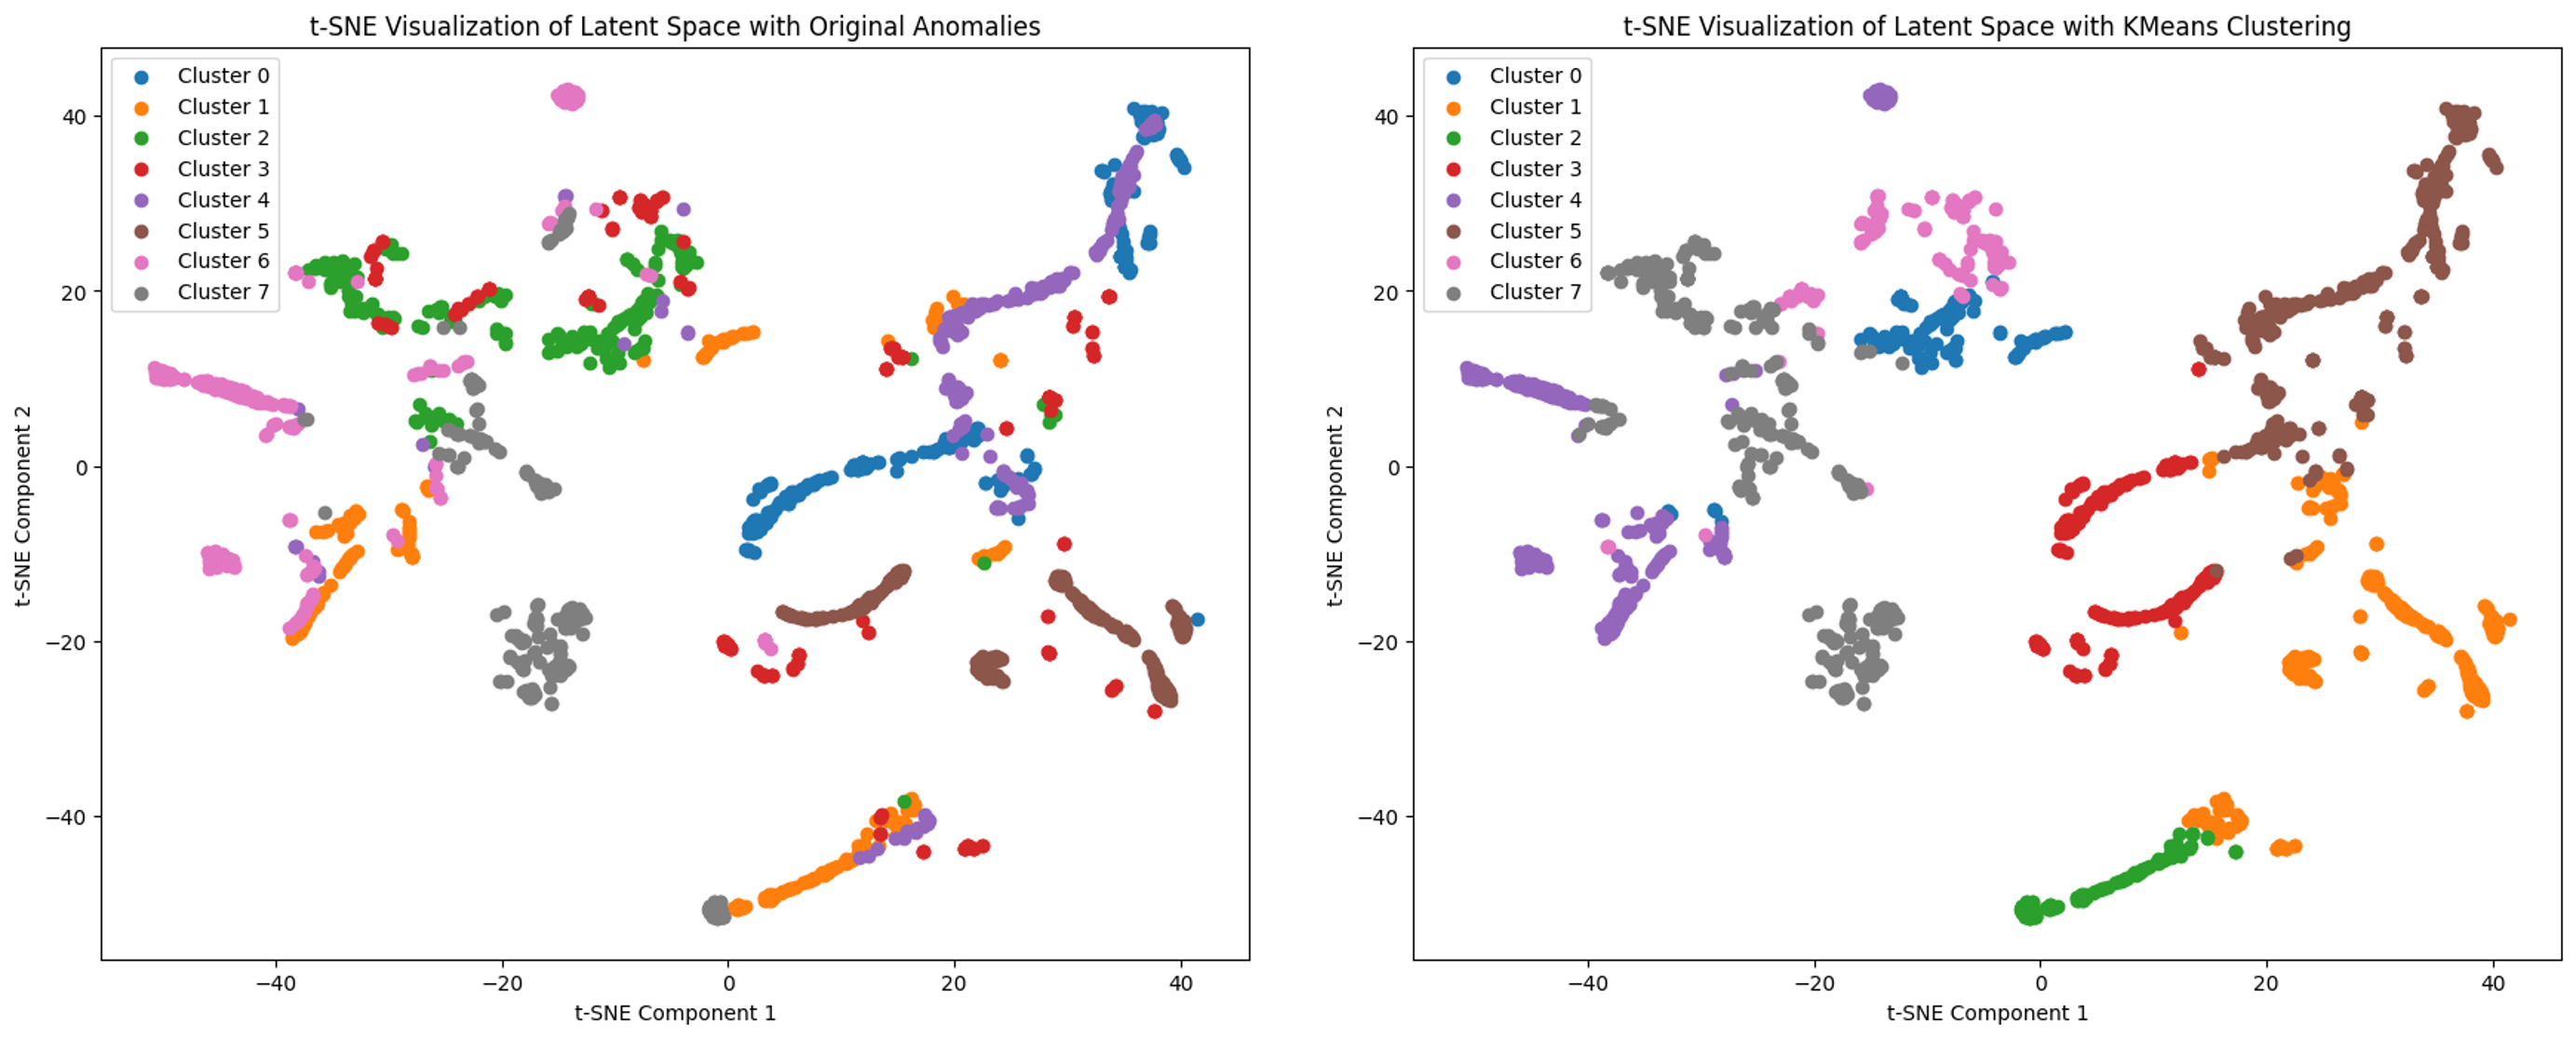
\includegraphics[width=\textwidth]{autoencoder_clustering.png}
\caption{Projeção t-SNE do espaço latente do codificador. À esquerda, os pontos coloridos
pelos oito rótulos originais do 3W; à direita, pelos agrupamentos obtidos com $K$-médias
sobre a mesma representação. A correspondência entre as duas partições é parcial: alguns
rótulos ocupam regiões bem definidas, outros se dispersam por vários agrupamentos.
Adaptado de \citet{Lopes2025EAAI}.}
\label{fig:aberto-agrupamento-latente}
\end{figure}

A \cref{fig:aberto-agrupamento-latente} antecipa esse diagnóstico. Se a representação
fosse o gargalo, o painel da direita seria uma versão embaralhada do da esquerda. Não é:
a estrutura existe, e o agrupamento a recupera em boa parte. O que falha é a
\emph{fronteira} entre classes vizinhas --- e nenhuma variante de autoencoder resolve
isso, porque todas otimizam reconstrução, e reconstrução não distingue vizinhos.

\begin{destaque}[A releitura pelo \cref{cap:mahalanobis}]
Há uma terceira interpretação, que só ficará disponível quando a evolução narrada na
\cref{parte:evolucao} for apresentada: talvez o problema não seja \emph{qual}
autoencoder, mas o fato de usar um autoencoder. O \cref{cap:mahalanobis} mostrará que o
espaço latente extraído da penúltima camada de um classificador multiclasse é
substancialmente melhor --- silhueta de $0{,}2299$ contra $-0{,}0149$ do autoencoder.
A razão é intuitiva em retrospecto: um autoencoder é treinado para \emph{reconstruir},
não para \emph{separar}.
\end{destaque}

\section{Etapas 2 e 3: reconhecer e rejeitar}

\subsection{Classificadores binários no espaço latente}

Sobre o vetor latente, um classificador binário por classe:

\begin{center}
\small
\begin{tabular}{ll}
\toprule
\textbf{Camada} & \textbf{Configuração} \\
\midrule
Entrada        & vetor latente \\
Densa(64)      & ReLU \\
\ing{Dropout}  & $0{,}3$ \\
Densa(32)      & ReLU \\
\ing{Dropout}  & $0{,}2$ \\
Densa(1)       & sigmoide \\
\bottomrule
\end{tabular}
\end{center}

Note a diferença em relação ao \cref{cap:binarios}: lá os classificadores recebiam a
série bruta e precisavam de camadas recorrentes; aqui recebem um vetor de dezesseis
dimensões e bastam camadas densas. O trabalho de extrair estrutura temporal foi
transferido para o autoencoder --- o que é, ao mesmo tempo, uma economia e um risco: o
que o autoencoder descartou está perdido para sempre.

\subsection{O voto ponderado}

Cada classe dispõe de dois escores: o do classificador binário, $s_i^{(b)}$, e o da
OCSVM ajustada aos dados daquela classe no latente, $s_i^{(o)}$. A decisão combina os
dois:
\begin{equation}
  S_i = w_i^{(b)} \, s_i^{(b)} + w_i^{(o)} \, s_i^{(o)},
  \qquad w_i^{(b)} + w_i^{(o)} = 1,
  \label{eq:aberto-voto}
\end{equation}
com rejeição quando $\max_i S_i < \tau$, $\tau = 0{,}65$.

Os pesos foram ajustados por classe, no conjunto de validação
(\cref{tab:aberto-pesos}).

\begin{table}[htbp]
\centering
\caption{Pesos do voto ponderado por classe. $w^{(b)}$ é o peso do classificador
binário e $w^{(o)}$ o da OCSVM.}
\label{tab:aberto-pesos}
\small
\begin{tabular}{lcc}
\toprule
\textbf{Classe} & $\bm{w^{(b)}}$ & $\bm{w^{(o)}}$ \\
\midrule
1 --- Aumento de BSW          & $0{,}65$ & $0{,}35$ \\
2 --- Fechamento de DHSV      & $0{,}54$ & $0{,}46$ \\
3 --- Golfadas severas        & $0{,}75$ & $0{,}25$ \\
4 --- Instabilidade de fluxo  & $0{,}52$ & $0{,}48$ \\
5 --- Perda de produtividade  & $0{,}58$ & $0{,}42$ \\
6 --- Restrição rápida no PCK & $0{,}77$ & $0{,}23$ \\
7 --- Incrustação no PCK      & $0{,}62$ & $0{,}38$ \\
8 --- Hidrato na produção     & $0{,}53$ & $0{,}47$ \\
9 --- Hidrato no serviço      & $0{,}54$ & $0{,}46$ \\
\midrule
Nenhuma (rejeição)            & $0{,}26$ & $\bm{0{,}74}$ \\
\bottomrule
\end{tabular}
\end{table}

\begin{destaque}[A linha mais informativa da tabela]
É a última. Para decidir que uma janela \emph{não pertence a nenhuma classe conhecida}, o
peso ótimo da OCSVM é $0{,}74$ --- quase três vezes o do classificador binário. Para
todas as outras decisões, a proporção se inverte.

A interpretação é direta e generaliza para além deste sistema: \textbf{classificadores
discriminativos são bons para dizer o que algo é; modelos de suporte, treinados apenas
sobre dados de uma classe, são bons para dizer o que algo não é}. Cada família de método
tem o seu papel, e tentar que uma delas cumpra os dois é o erro que o
\cref{cap:introducao} descreveu.
\end{destaque}

\subsection{Desempenho dos classificadores binários latentes}

A \cref{tab:aberto-binarios} reporta o desempenho por classe em dois níveis de
granularidade discutidos no \cref{cap:aprendizado}.

\begin{table}[htbp]
\centering
\caption{Desempenho dos classificadores binários no espaço latente. As duas primeiras
colunas referem-se ao experimento consolidado; as duas últimas, à média e ao desvio
padrão entre execuções, por amostra e por instância.}
\label{tab:aberto-binarios}
\small
\begin{tabular}{lcccc}
\toprule
\textbf{Classe} & \textbf{ACC} & $\bm{F_1}$ & \textbf{ACC (méd.\,$\pm$\,dp)} &
\textbf{Instância (méd.\,$\pm$\,dp)} \\
\midrule
1 & $0{,}92$ & $0{,}93$ & $0{,}82 \pm 0{,}04$ & $1{,}00$ \\
2 & $0{,}90$ & $0{,}90$ & $0{,}85 \pm 0{,}03$ & $0{,}98 \pm 0{,}05$ \\
3 & $0{,}85$ & $0{,}87$ & $0{,}89 \pm 0{,}02$ & $1{,}00$ \\
4 & $0{,}69$ & $0{,}68$ & $0{,}64 \pm 0{,}03$ & $1{,}00$ \\
5 & $0{,}82$ & $0{,}83$ & $0{,}75 \pm 0{,}03$ & $0{,}76 \pm 0{,}05$ \\
6 & $0{,}94$ & $0{,}95$ & $0{,}75 \pm 0{,}13$ & $0{,}34 \pm 0{,}42$ \\
7 & $0{,}79$ & $0{,}83$ & $0{,}80 \pm 0{,}01$ & $1{,}00$ \\
8 & $0{,}90$ & $0{,}91$ & $0{,}80 \pm 0{,}06$ & $0{,}94 \pm 0{,}12$ \\
9 & $0{,}92$ & $0{,}92$ & $0{,}81 \pm 0{,}05$ & $1{,}00$ \\
\bottomrule
\end{tabular}
\end{table}

Três observações.

A classe 4 permanece a pior, com $0{,}69$ --- \emph{exatamente} o mesmo valor obtido no
\cref{cap:binarios} sobre o espaço bruto. Mudar a representação não mudou nada, o que
reforça o diagnóstico de que o problema está no rótulo.

A classe 6 exibe a patologia mais interessante da tabela: acurácia por amostra de
$0{,}75 \pm 0{,}13$, mas acurácia por instância de $0{,}34 \pm 0{,}42$. Um desvio padrão
de $0{,}42$ sobre uma média de $0{,}34$ significa que o classificador acerta a instância
inteira ou erra a instância inteira, sem meio-termo, dependendo da execução. É um
classificador instável, e a métrica por amostra o esconde.

\begin{destaque}[Por que reportar os dois níveis]
Sete das nove classes atingem acurácia por instância de $0{,}94$ ou mais, contra
acurácias por amostra entre $0{,}64$ e $0{,}89$. Reportar apenas o nível de instância
sugeriria um sistema quase perfeito; reportar apenas o nível de amostra sugeriria um
sistema medíocre. Ambos são verdadeiros e respondem a perguntas operacionais
diferentes: ``o sistema identifica o evento?'' e ``o sistema delimita o evento?''.
\end{destaque}

\section{O teste real: a anomalia de ICV}

Toda a discussão anterior seria acadêmica sem uma anomalia genuinamente inédita. Ela
existe: a falha em válvula de controle de intervalo (ICV), descrita no
\cref{cap:dominio}, que \emph{não pertence a nenhuma das nove classes do 3W} e cujos
dados são de poços reais.

\subsection{Como o ensemble reage}

\begin{figure}[htbp]
\centering
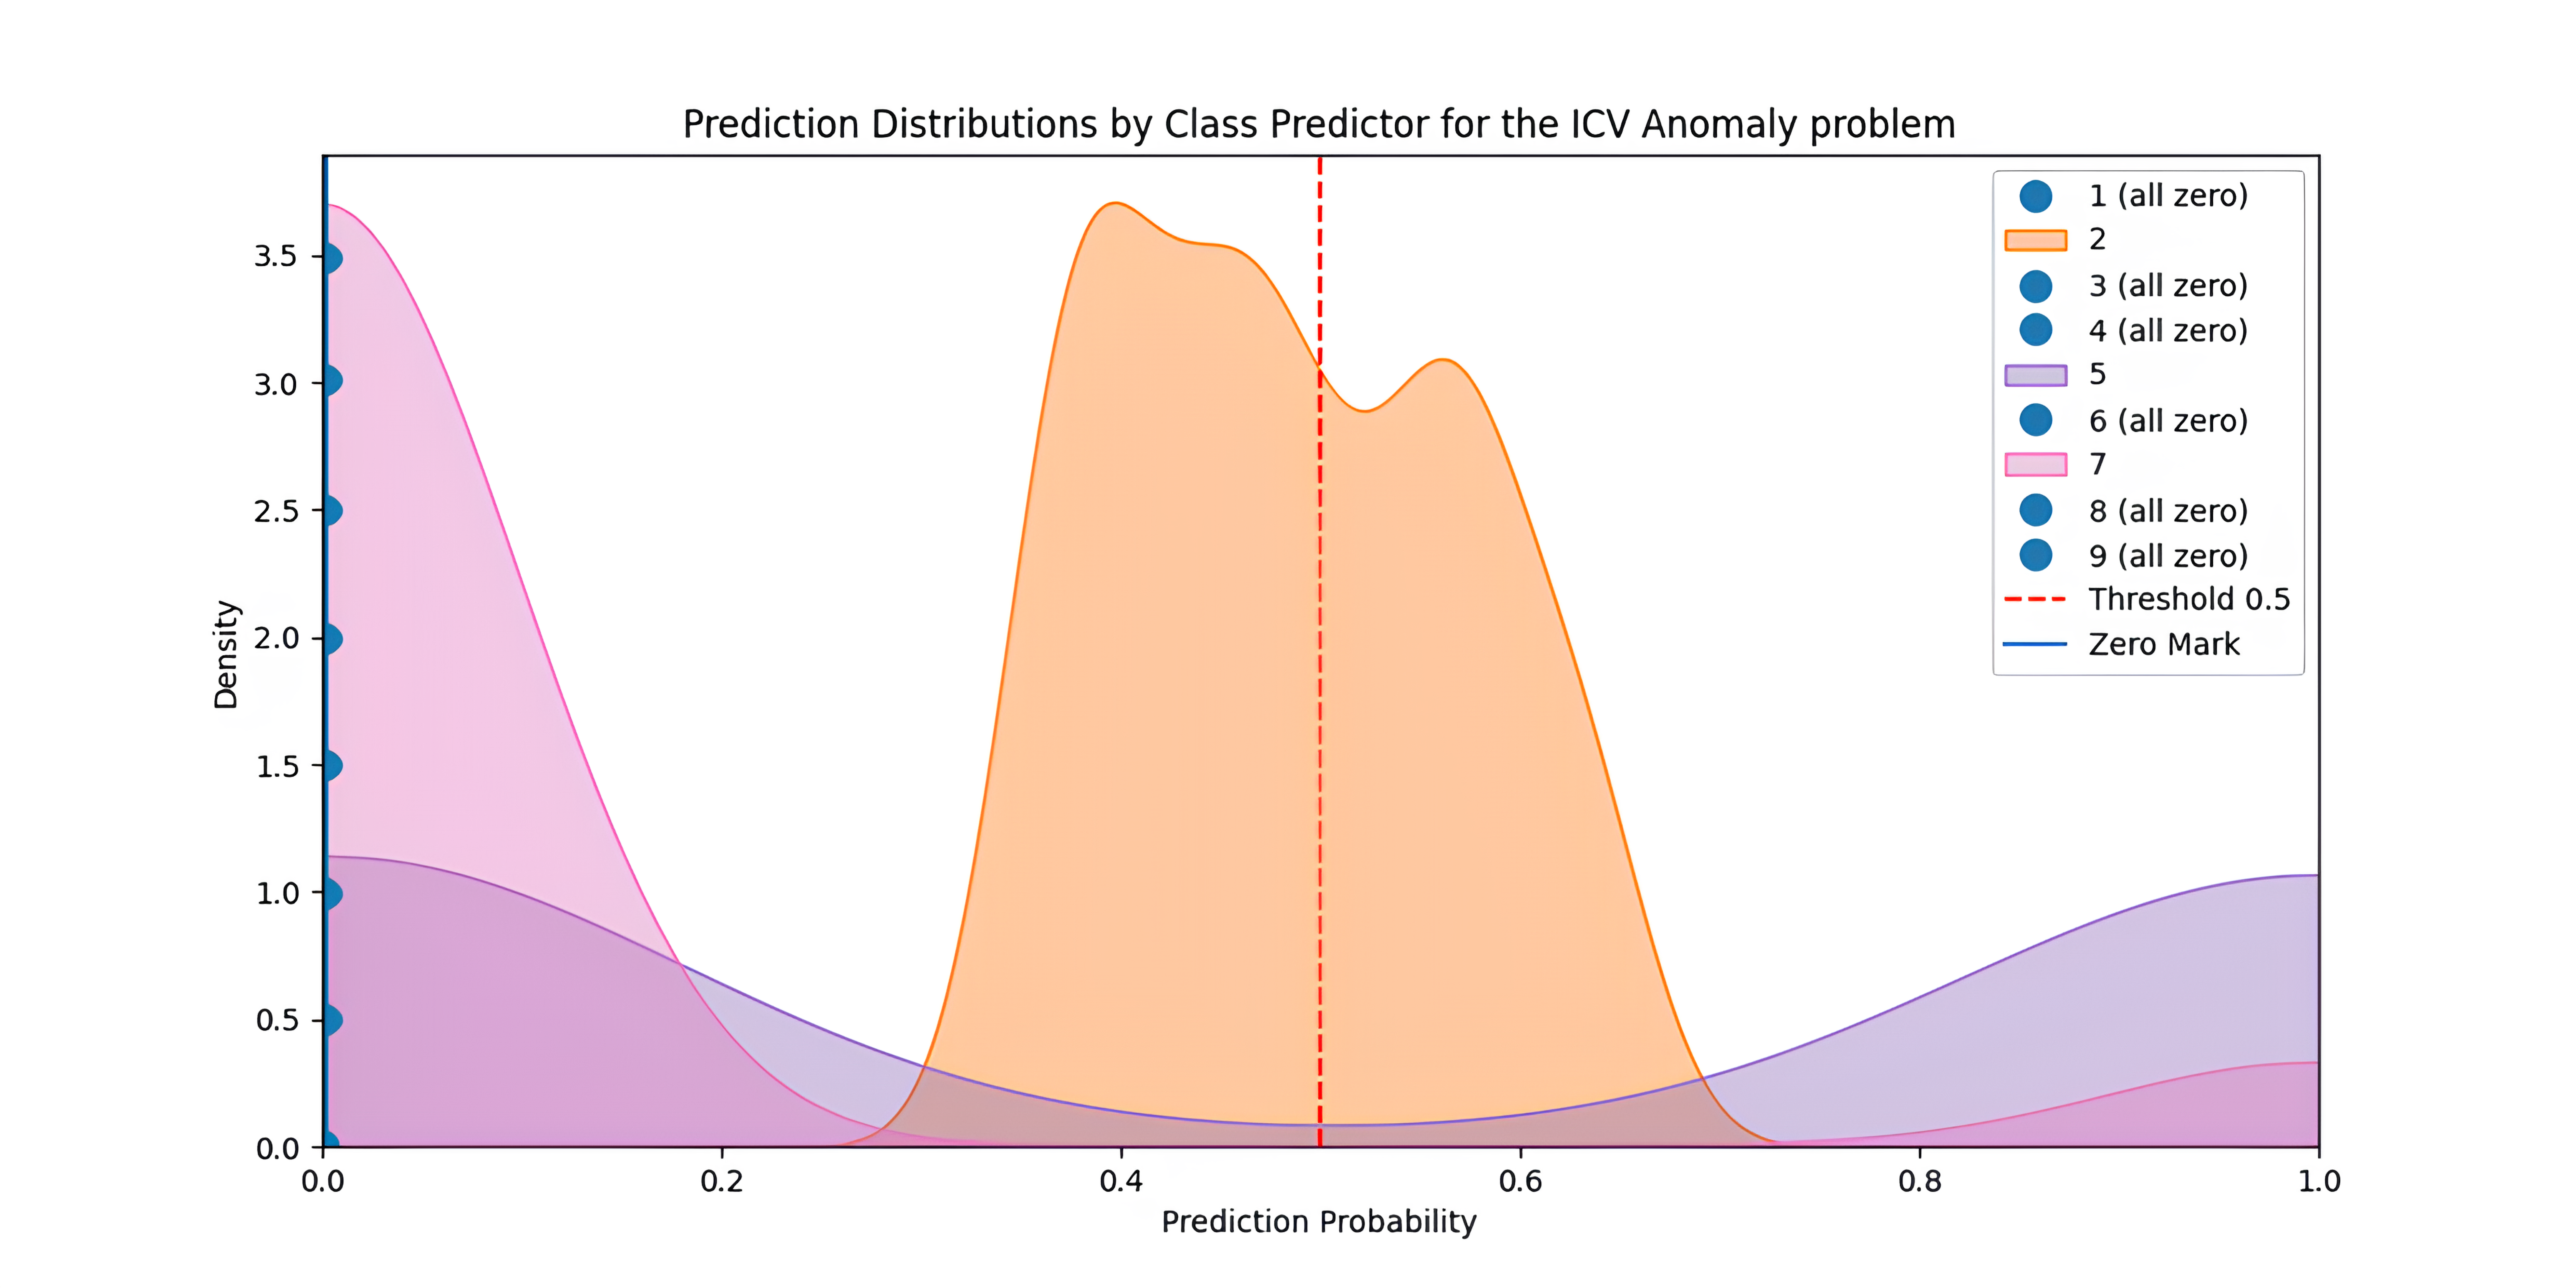
\includegraphics[width=\textwidth]{classifier_with_ICV_improved.png}
\caption{Distribuição dos escores dos nove classificadores binários quando apresentados
a janelas da anomalia de ICV --- uma classe que nenhum deles conhece. Seis dos nove
(1, 3, 4, 6, 8 e 9) produzem escore identicamente nulo. O classificador da classe 2
concentra-se em torno do limiar $0{,}5$, sem decidir. Os classificadores das classes 5 e
7 distribuem massa acima do limiar. A linha tracejada indica o limiar de decisão.
Adaptado de \citet{Lopes2025EAAI}.}
\label{fig:aberto-icv-classificadores}
\end{figure}

A \cref{fig:aberto-icv-classificadores} é uma das figuras mais informativas deste livro,
porque mostra simultaneamente o sucesso e o limite da rejeição.

O sucesso: seis dos nove classificadores respondem \emph{zero absoluto}. Não é
incerteza --- é recusa. O comportamento é exatamente o que a formulação um-contra-todos
do \cref{cap:binarios} prometia e que uma \ing{softmax} jamais poderia produzir, já que
os escores somariam um por construção.

O limite: os classificadores das classes 5 e 7 --- perda de produtividade e incrustação
--- atribuem probabilidade alta a parte das janelas. E a explicação, novamente, é
física, não algorítmica: uma ICV com falha \emph{de fato} restringe fluxo e \emph{de
fato} reduz produtividade. A assinatura sintomática é compartilhada. O classificador não
está errado no que observa; o rótulo é que não distingue causa de efeito.

\begin{resultadochave}
Do total de janelas de ICV, $\bm{48\,\%}$ foram atribuídas a alguma classe conhecida ---
majoritariamente 5 e 7 --- e $\bm{52\,\%}$ foram corretamente rejeitadas e encaminhadas
ao agrupamento.
\end{resultadochave}

Metade de uma anomalia genuinamente nova é reconhecida como nova. É simultaneamente um
resultado forte --- comparado a zero, que é o que um classificador de mundo fechado
entregaria --- e um resultado que deixa clara a distância até um sistema confiável.

\section{Etapas 4 e 5: agrupar, refinar, validar}

\subsection{Estimar o número de grupos}

Antes de agrupar é preciso decidir em quantos grupos. A solução adotada evita tanto o
arbítrio quanto a inspeção visual do cotovelo: uma \textbf{floresta aleatória} treinada
para prever $K$ a partir de oito características do próprio conjunto de dados.

\begin{center}
\small
\begin{tabular}{ll}
\toprule
\textbf{Característica} & \textbf{Descrição} \\
\midrule
$n$                    & número de amostras \\
Silhueta               & \cref{eq:silhueta} \\
Davies-Bouldin         & \cref{eq:db} \\
Calinski-Harabasz      & razão de dispersão entre e intra grupos \\
Inércia                & soma dos quadrados intra grupo \\
\texttt{avg\_k}        & estimativa por média de índices \\
\texttt{entropy\_k}    & estimativa por entropia da distribuição \\
Volume do envoltório   & hipervolume da caixa delimitadora dos dados \\
\bottomrule
\end{tabular}
\end{center}

A estimativa final é a média de duas delas:
\begin{equation}
  \hat{K} = \frac{\texttt{avg\_k} + \texttt{entropy\_k}}{2}.
  \label{eq:aberto-k}
\end{equation}

\begin{table}[htbp]
\centering
\caption{Indicadores do estimador do número de agrupamentos reportados por
\citet{Lopes2025EAAI}.}
\label{tab:aberto-rf}
\begin{tabular}{lc}
\toprule
\textbf{Métrica} & \textbf{Valor publicado} \\
\midrule
Acurácia                   & $98{,}3\,\%$ \\
Precisão                   & $0{,}98$ \\
Revocação                  & $0{,}86$ \\
Medida $F_1$               & $0{,}87$ \\
Erro médio absoluto em $K$ & $1{,}12$ \\
\bottomrule
\end{tabular}
\end{table}

\begin{destaque}[Resultado publicado e verificação independente]
A \cref{tab:aberto-rf} preserva os valores publicados e os atribui à fonte primária;
ela não é uma reprodução independente. Se ``acurácia'' significar acerto exato de $K$
e o MAE usar as mesmas predições, os dois indicadores não passam por uma verificação
aritmética: os $1{,}7\,\%$ de casos incorretos teriam erro absoluto médio condicionado de
$1{,}12/0{,}017\approx65{,}9$ grupos. Esse valor é incompatível com a escala descrita
para a tarefa.

As explicações possíveis incluem denominadores distintos, outra definição de acurácia,
MAE calculado para um componente intermediário ou erro de transcrição. Sem as predições
por conjunto ou material suplementar, não é possível escolher entre elas. Portanto, os
valores podem ser citados individualmente como resultados do artigo, mas não sustentam
a conclusão de que o estimador acerta exatamente $K$ em $98{,}3\,\%$ dos casos e erra,
em média, apenas um grupo quando falha.
\end{destaque}

\subsection{Interseção entre dois algoritmos}

O agrupamento não é confiado a um único método. Executam-se \textbf{K-means} --- com o
$K$ estimado --- e \textbf{MeanShift}, cuja largura de banda é determinada pelos próprios
dados, e retêm-se as amostras em que os dois concordam.

\begin{figure}[htbp]
\centering
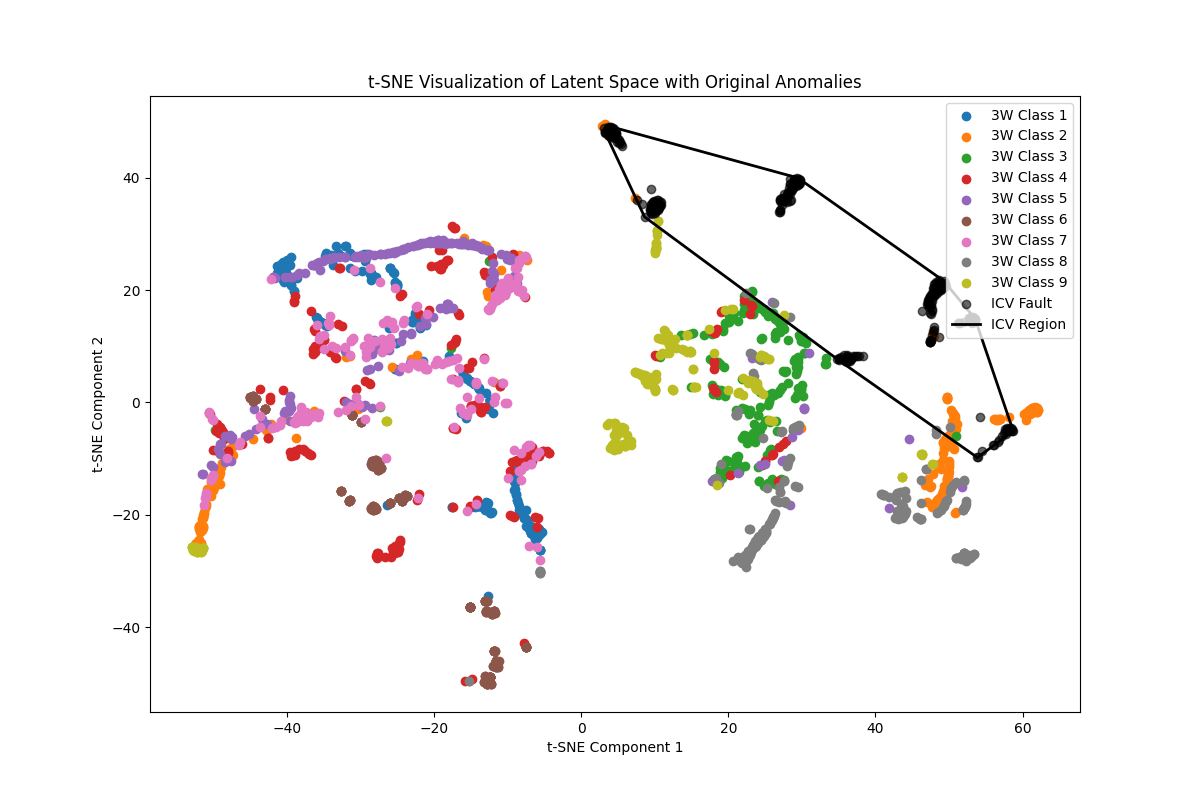
\includegraphics[width=0.85\textwidth]{latent_space_with_ICV_corrected.png}
\caption{Projeção t-SNE do espaço latente. Cada cor corresponde a um agrupamento
identificado pelo K-means sobre as classes conhecidas; os círculos vermelhos são as
janelas de ICV rejeitadas, e a região sombreada é o envoltório convexo que elas ocupam.
Note que as janelas de ICV não formam um grupo compacto: elas se distribuem em subgrupos
separados, no limite entre agrupamentos existentes. Adaptado de \citet{Lopes2025EAAI}.}
\label{fig:aberto-latente}
\end{figure}

\begin{figure}[htbp]
\centering
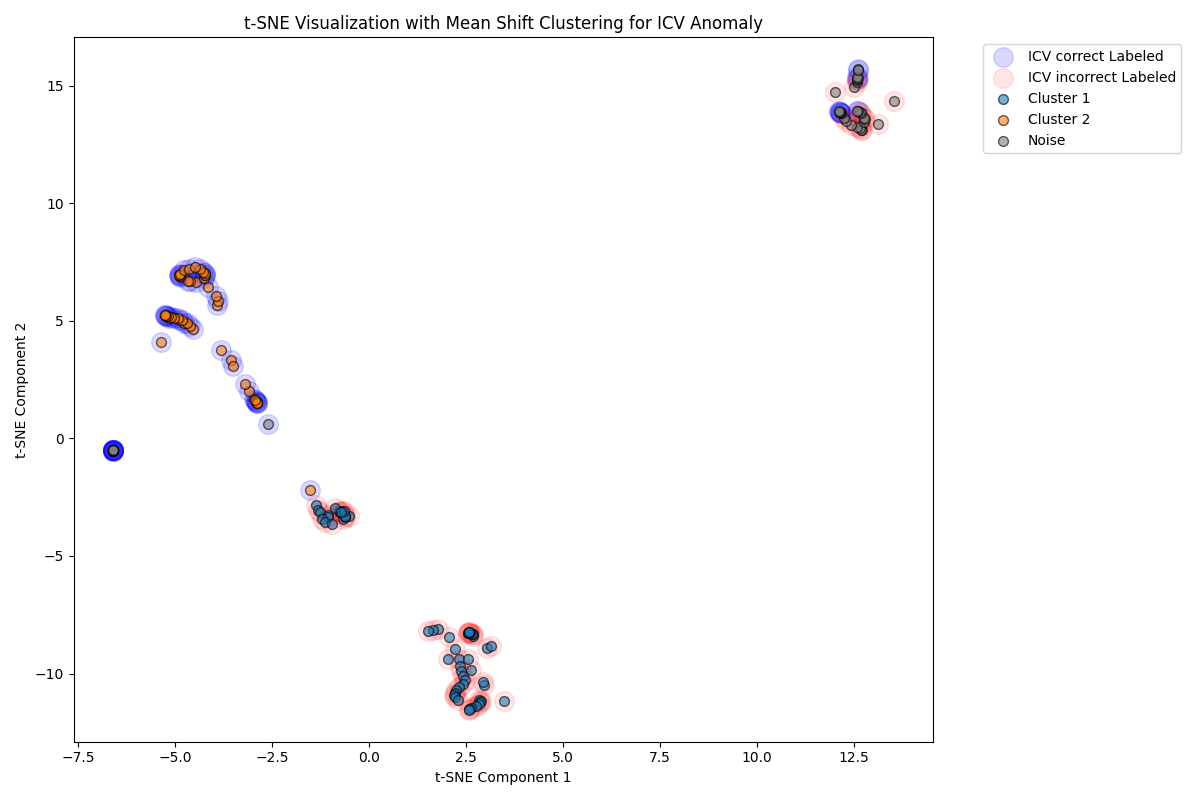
\includegraphics[width=0.85\textwidth]{meanshift_with_ICV_corrected.png}
\caption{Agrupamento das janelas de ICV rejeitadas por MeanShift, projetado por t-SNE.
O algoritmo identifica dois grupos e marca como ruído as amostras que não pertencem a
nenhum deles --- comportamento desejável, já que a rejeição inevitavelmente arrasta
janelas de transição. Adaptado de \citet{Lopes2025EAAI}.}
\label{fig:aberto-meanshift}
\end{figure}

\begin{figure}[htbp]
\centering
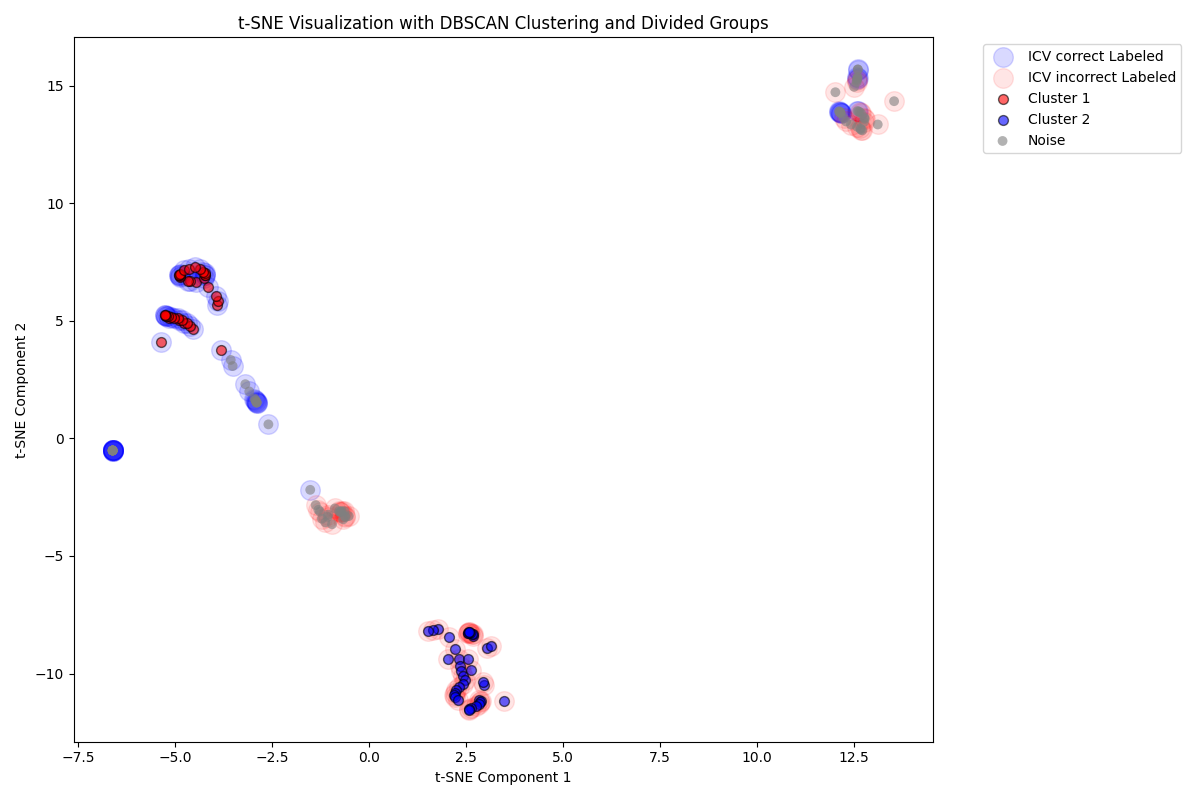
\includegraphics[width=0.85\textwidth]{dbscan_with_ICV_corrected.png}
\caption{Agrupamento das mesmas janelas por DBSCAN. O algoritmo não exige que se declare
o número de grupos, mas transfere a dificuldade para os parâmetros $\varepsilon$ e
$\mathit{minPts}$: com a densidade heterogênea do espaço latente, ele ou funde os
subgrupos ou classifica a maior parte das amostras como ruído. Adaptado de
\citet{Lopes2025EAAI}.}
\label{fig:aberto-dbscan}
\end{figure}

A comparação entre as \cref{fig:aberto-latente,fig:aberto-meanshift} explica por que a
interseção é necessária. Os dois algoritmos partem de premissas diferentes --- o K-means
supõe grupos esféricos de tamanho comparável; o MeanShift, modos de densidade --- e a
concordância entre eles é um indício de estrutura genuína, não de artefato do método.
A \cref{fig:aberto-dbscan} mostra o terceiro candidato descartado: o DBSCAN é o método
teoricamente mais adequado a grupos de forma arbitrária, mas neste espaço latente sua
sensibilidade a $\varepsilon$ o torna instável demais para uso automático.

\begin{destaque}[Uma advertência sobre o t-SNE]
As \cref{fig:aberto-latente,fig:aberto-meanshift} são projeções t-SNE, e o
\cref{cap:novidades} advertiu: distâncias no t-SNE não são distâncias no latente, e o
algoritmo produz agrupamentos visualmente convincentes mesmo em ruído puro. Estas
figuras servem para \emph{ilustrar}, nunca para \emph{provar}. A evidência quantitativa
está nos índices internos e nas taxas de acerto.
\end{destaque}

\subsection{Refinamento por limiar adaptativo}

Nem toda amostra atribuída a um grupo pertence a ele. Aplica-se, dentro de cada grupo,
um limiar sobre a distância ao centroide:
\[
  T = \mu + k\sigma,
\]
com $k$ determinado pela razão $R = \mu / \sigma$ da distribuição de distâncias:
\begin{equation}
  k = \begin{cases}
    2, & \text{se } R \geq 4, \\[0.2em]
    1 + \dfrac{R-2}{2}, & \text{se } 2 \leq R < 4, \\[0.5em]
    0, & \text{se } R < 2.
  \end{cases}
  \label{eq:aberto-kadaptativo}
\end{equation}

A lógica é a seguinte. $R$ alto indica grupo compacto e homogêneo, e nesse caso pode-se
ser tolerante ($k = 2$). $R$ baixo indica grupo disperso, provavelmente contaminado, e
exige rigor ($k = 0$, ou seja, retém-se apenas o que está abaixo da distância média).
Entre os dois extremos, interpola-se linearmente.

Uma salvaguarda final: se o critério eliminar mais de dois terços do grupo, ele é
descartado e mantêm-se os dois terços mais próximos do centroide. Sem essa proteção, um
grupo mal formado poderia ser reduzido a um punhado de amostras e ainda assim promovido
a classe.

\subsection{Validação}

Grupos sobreviventes são avaliados pelos índices internos do \cref{cap:novidades}:
silhueta, Davies-Bouldin e Calinski-Harabasz. Um grupo só é promovido a classe virtual
se apresentar coesão e separação adequadas segundo os três.

\subsection{O que o agrupamento acerta, quando acerta}

A acurácia agregada esconde uma variabilidade grande entre combinações de classes
desconhecidas. Vale examinar um caso favorável para saber o que o método produz quando
as condições lhe são proprícias.

\begin{figure}[htbp]
\centering
\begin{minipage}{0.49\textwidth}
  \centering
  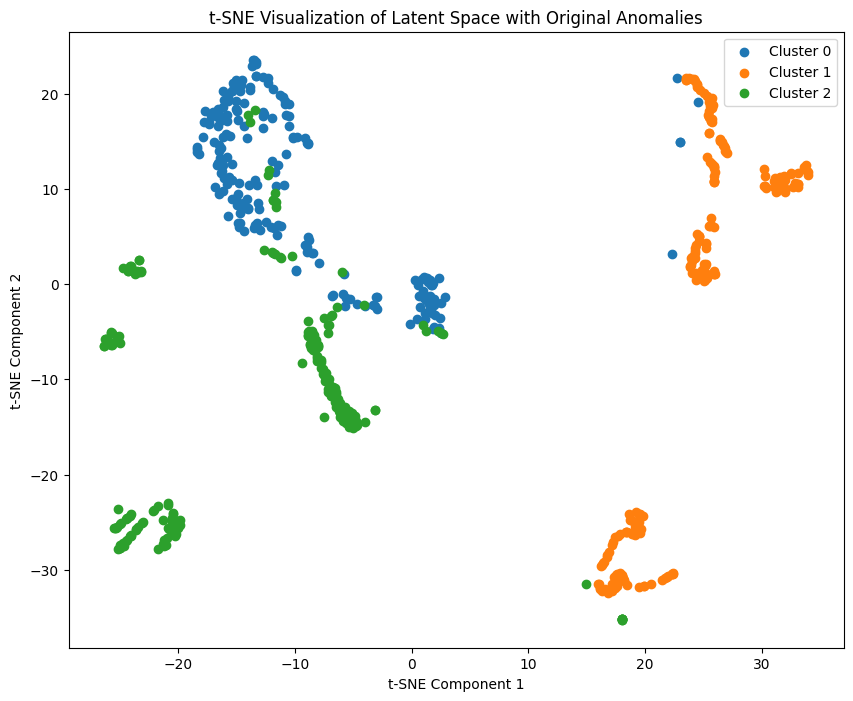
\includegraphics[width=\textwidth]{best_original.png}
\end{minipage}\hfill
\begin{minipage}{0.49\textwidth}
  \centering
  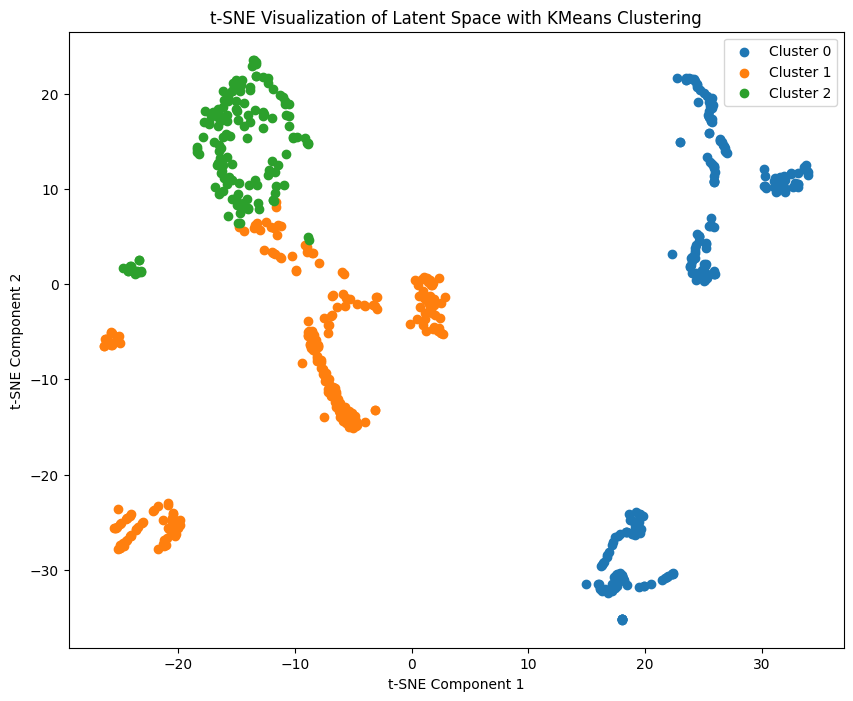
\includegraphics[width=\textwidth]{best_clustering.png}
\end{minipage}
\caption{Ocultando as classes 3, 6 e 8 e tratando-as como desconhecidas. À esquerda, a
distribuição original dos dados, colorida pelos rótulos verdadeiros; à direita, os três
agrupamentos recuperados por $K$-médias sem acesso a esses rótulos. Adaptado de
\citet{Lopes2025EAAI}.}
\label{fig:aberto-melhor-caso}
\end{figure}

A \cref{fig:aberto-melhor-caso} mostra esse caso: escondem-se três das nove classes
conhecidas, treina-se o sistema com as seis restantes e verifica-se o que o agrupamento
faz com o material rejeitado. A correspondência entre os dois painéis é boa --- medida
$F_1$ de $0{,}71$, $0{,}97$ e $0{,}76$ para as classes 3, 6 e 8 --- e o número de grupos
foi estimado corretamente.

\begin{figure}[htbp]
\centering
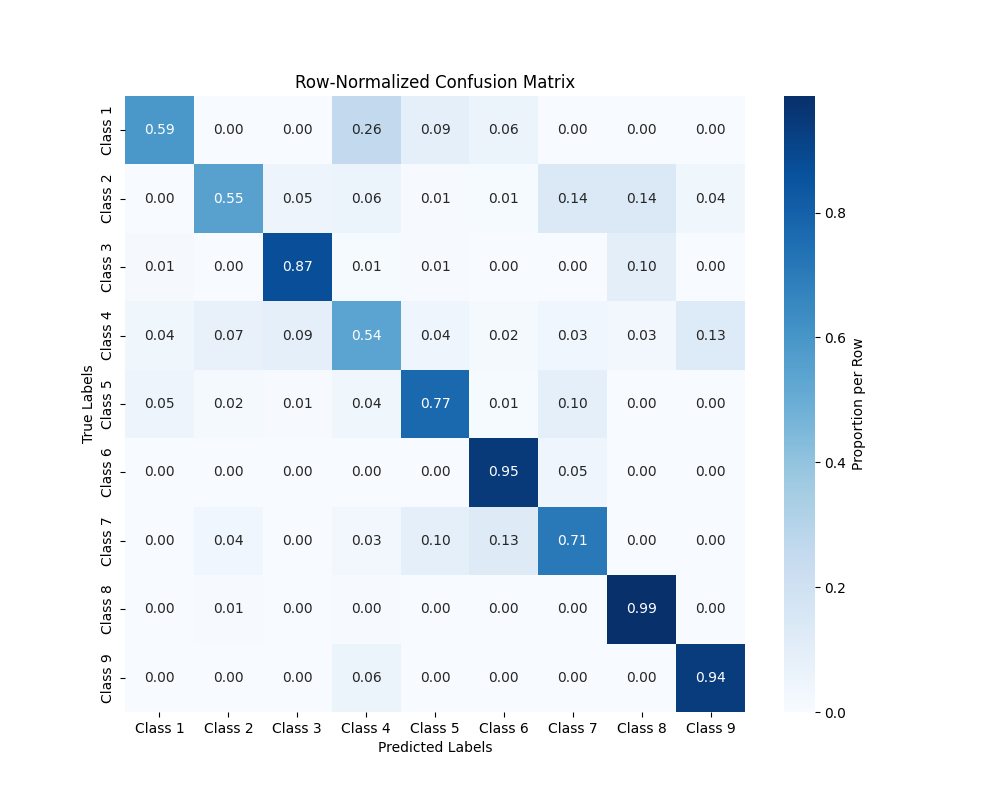
\includegraphics[width=0.78\textwidth]{confusion_matrix_kmeans.png}
\caption{Matriz de confusão normalizada do agrupamento por $K$-médias, agregada sobre as
$\binom{9}{3} = 168$ combinações possíveis de três classes ocultas. A diagonal domina,
mas os erros não estão distribuídos de modo uniforme. Adaptado de
\citet{Lopes2025EAAI}.}
\label{fig:aberto-matriz-kmeans}
\end{figure}

Um caso favorável, contudo, não é evidência. Por isso o experimento foi repetido para
\emph{todas} as $168$ combinações de três classes escolhidas entre nove, e a
\cref{fig:aberto-matriz-kmeans} agrega o resultado. A leitura importante não é a
diagonal, e sim o padrão fora dela: os erros concentram-se nos mesmos pares que já
haviam aparecido na \cref{fig:aberto-latente} e na rejeição da anomalia de ICV. Não é
ruído do algoritmo --- é sobreposição real de assinatura entre classes vizinhas, e nenhum
método de agrupamento a desfaz sozinho.

\section{Etapa 6: classes virtuais}

\begin{definicao}{Classe virtual}
Agrupamento validado que passa a ser tratado como classe pelo sistema, recebendo seu
próprio classificador binário, mas que ainda não foi nomeado nem confirmado por um
especialista.
\end{definicao}

A promoção a classe virtual é a etapa que fecha o ciclo, e ela é barata precisamente por
causa da propriedade de extensibilidade incremental estabelecida no \cref{cap:binarios}:
treina-se um novo classificador binário, e nenhum dos existentes é tocado.

\begin{figure}[htbp]
\centering
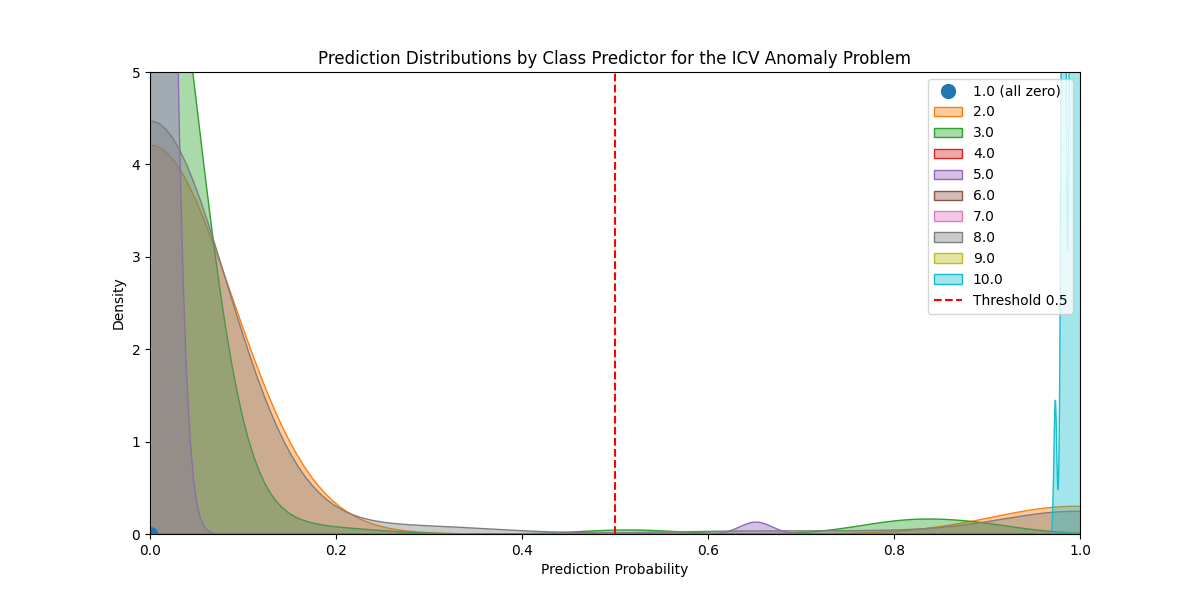
\includegraphics[width=\textwidth]{classifier_with_ICV_with_10_classes.png}
\caption{O mesmo cenário da \cref{fig:aberto-icv-classificadores}, agora com dez
classificadores. O décimo foi treinado exclusivamente sobre as janelas antes rejeitadas
e reivindica a maior parte delas; as reivindicações espúrias das classes 2 e 5
retrocedem. Adaptado de \citet{Lopes2025EAAI}.}
\label{fig:aberto-dez-classes}
\end{figure}

A \cref{fig:aberto-dez-classes} é o fecho experimental do ciclo, e deve ser lida em par
com a \cref{fig:aberto-icv-classificadores}. São os mesmos dados de ICV apresentados ao
mesmo conjunto de classificadores, com uma única diferença: um décimo classificador foi
acrescentado, treinado apenas com o material que o próprio sistema havia separado como
desconhecido. O que era detecção dispersa entre duas classes erradas torna-se uma
reivindicação concentrada e correta --- a validação de que $0{,}98$ de acurácia na
décima classe não custou desempenho nas nove anteriores.

\begin{destaque}[O que esta figura não prova]
O décimo classificador aprendeu a reconhecer a falha de ICV, mas ninguém lhe disse que
aquilo \emph{era} uma falha de ICV. Para o sistema, a classe continua anônima: um
agrupamento coerente, reprodutível e agora reconhecível, sem nome nem causa.

Nomear é outro problema, e é exatamente onde começa a \cref{parte:explicabilidade}.
\end{destaque}

\begin{resultadochave}
Sobre o conjunto de janelas rejeitadas, o ciclo de agrupamento e refinamento atinge
acurácia de $\bm{80{,}8\,\%}$ no nível de amostra na atribuição a grupos coerentes.
\end{resultadochave}

\section{Balanço}

O ciclo funciona, e funciona parcialmente. Vale enunciar as duas metades com igual
clareza.

\textbf{O que funciona.} A rejeição não é uma promessa teórica: $52\,\%$ de uma anomalia
genuinamente inédita foram identificados como tal, com seis de nove classificadores
respondendo zero absoluto. O agrupamento subsequente organiza esse material com
$80{,}8\,\%$ de acurácia. A estimativa automática de $K$ dispensa arbítrio. E o
mecanismo de classes virtuais permite crescimento do repertório sem retreinamento
global.

\textbf{O que não funciona.} Quase metade das janelas de ICV foi absorvida pelas classes
sintomáticas 5 e 7. A escolha da representação --- autoencoder, VAE ou DCN --- é
irrelevante, o que sugere que o gargalo não foi identificado. As classes 4 e 5 falham
sistematicamente. E, sobretudo, \textbf{as classes virtuais não têm nome}: o sistema
produz ``grupo 11'', não ``falha de ICV''.

\begin{destaque}[As três portas que este capítulo abre]
Cada uma dessas limitações define uma das partes seguintes do livro.

A representação inadequada leva ao \cref{cap:mahalanobis}: o latente do classificador
multiclasse supera o do autoencoder por uma margem que torna o resultado da
\cref{tab:aberto-arquiteturas} compreensível em retrospecto.

A detecção grosseira, no nível de janela inteira, leva ao \cref{cap:segmentacao}: uma
U-Net que segmenta ponto a ponto, elevando a acurácia de $0{,}500$ para $0{,}863$.

E a ausência de nomes leva à \cref{parte:explicabilidade}, onde um modelo de linguagem
recebe as estatísticas do segmento anômalo e produz uma descrição em linguagem natural
--- que, para a maioria das classes, converge para um nome consistente.
\end{destaque}

\resumocapitulo{%
O ciclo de aprendizado de mundo aberto tem seis etapas: representação, reconhecimento,
rejeição, agrupamento, refinamento e incorporação. A representação é um autoencoder LSTM
que comprime $200 \times 4$ valores em dezesseis dimensões; alternativas variacionais e
de \ing{clustering} profundo produzem desempenho estatisticamente indistinguível
($0{,}730$, $0{,}727$ e $0{,}725$), o que indica que o gargalo está em outro lugar. A
rejeição combina classificadores binários e OCSVM em um voto ponderado por classe, e o
peso ótimo da OCSVM na decisão de rejeitar é $0{,}74$ contra $0{,}26$ do classificador
--- evidência de que reconhecer e rejeitar são tarefas para famílias distintas de
método. Sobre uma anomalia genuinamente inédita, a falha de ICV, seis dos nove
classificadores produzem escore nulo e $52\,\%$ das janelas são corretamente rejeitadas;
os $48\,\%$ restantes são absorvidos pelas classes sintomáticas 5 e 7. O agrupamento usa
a interseção entre K-means e MeanShift, com $K$ estimado por uma floresta aleatória
sobre oito índices. O artigo reporta $98{,}3\,\%$ de acurácia e MAE de $1{,}12$, valores
preservados aqui com a ressalva de que suas definições conjuntas aguardam reconciliação
a partir das predições por conjunto. O refinamento usa um limiar adaptativo
$\mu + k\sigma$ com $k$ dependente da razão
$R = \mu/\sigma$. A acurácia do ciclo de agrupamento é de $80{,}8\,\%$ no nível de
amostra. Os grupos validados tornam-se classes virtuais --- que ainda não têm nome.}

\begin{exercicios}
\item O peso ótimo da OCSVM na decisão de rejeição é $0{,}74$, contra valores entre
      $0{,}23$ e $0{,}48$ nas decisões de reconhecimento. Explique essa assimetria em
      termos da natureza discriminativa dos classificadores binários e da natureza
      generativa dos modelos de suporte.

\item Implemente o limiar adaptativo da \cref{eq:aberto-kadaptativo}. Gere conjuntos
      sintéticos com diferentes graus de dispersão e verifique se o comportamento de $k$
      corresponde à intenção declarada. Proponha e avalie uma alternativa contínua e
      diferenciável.

\item Mostre que, se a acurácia de acerto exato de $K$ é $a$ e o erro médio absoluto é
      $m$, então o erro absoluto médio condicionado aos casos incorretos é
      $m/(1-a)$. Use essa identidade para propor verificações de consistência para um
      relatório que apresente as duas métricas.

\item \textbf{Projeto de extensão.} Com acesso aos dados e a um protocolo explicitamente
      versionado, substitua o autoencoder por um \ing{transformer} de séries temporais e
      compare-o com a \cref{tab:aberto-arquiteturas}. As diferenças entre representações
      permanecem pequenas? Documente por que seus valores podem divergir dos publicados e
      o que o resultado implica sobre onde concentrar esforço de engenharia.

\item A interseção entre K-means e MeanShift descarta amostras em que os dois algoritmos
      discordam. Quantifique, sobre o 3W, a fração descartada. Discuta o compromisso
      entre pureza dos grupos e cobertura, e proponha um critério para decidir quando a
      interseção é preferível à união.

\item Argumenta-se que $48\,\%$ das janelas de ICV foram absorvidas pelas classes 5 e 7
      por compartilharem assinatura sintomática. Projete um experimento que teste essa
      hipótese contra a alternativa de que se trata de simples limitação do
      classificador.

\item Uma classe virtual é promovida sem nome nem confirmação humana. Discuta os riscos
      operacionais de acumular classes virtuais indefinidamente e proponha uma política
      de governança: quando promover, quando fundir, quando descartar, e com que
      frequência solicitar revisão humana.
\end{exercicios}

\begin{leituras}
\item \citet{LopesTese2025} --- a tese que originou este capítulo, com detalhamento
      completo do ciclo.
\item \citet{Lopes2025EAAI} --- o artigo em que o ciclo foi publicado, origem das
      figuras deste capítulo.
\item \citet{openworld1}, \citet{openworld2} e \citet{openworld3} --- os fundamentos do
      aprendizado de mundo aberto.
\item \citet{Pimentel2014review} --- revisão abrangente de detecção de novidade.
\item \citet{Breiman2001} --- florestas aleatórias, aqui usadas de forma incomum, como
      estimador de metaparâmetro.
\item \citet{maaten2008visualizing} --- o t-SNE, com a discussão original sobre o que
      suas projeções podem e não podem sustentar.
\end{leituras}


\part{A evolução}\label{parte:evolucao}
\chapter{Superando o mundo fechado}
\label{cap:closedworld}

\begin{objetivos}
Ao final deste capítulo, você será capaz de:
\begin{itemize}[leftmargin=*,itemsep=0.2em]
      \item descrever e interpretar um experimento de mundo aberto por classe escondida;
  \item analisar o compromisso entre comprimento de janela, acurácia e tempo de resposta
        operacional;
  \item interpretar a validação de um classificador contra um modelo físico independente
        e analisar as discrepâncias;
  \item estimar o custo computacional de um ensemble e discutir sua viabilidade no
        ambiente avaliado;
  \item posicionar corretamente as limitações de um resultado positivo.
\end{itemize}
\end{objetivos}

\section{Do princípio à evidência}

O \cref{cap:binarios} estabeleceu que um ensemble de classificadores binários
\emph{pode} rejeitar, sem perda observada na acurácia agregada daquele experimento.
Faltava confrontá-lo com uma classe que o sistema realmente nunca viu e medir se a
rejeição continuava útil nesse protocolo.

Este capítulo apresenta essa evidência para uma classe escondida, junto com três investigações que a
acompanham: a varredura sistemática do comprimento de janela, a validação contra um
modelo termodinâmico independente e a análise do custo computacional. É o
aprofundamento do \cref{cap:binarios} --- mesmos classificadores, perguntas mais duras.

\section{O experimento da classe escondida}

\subsection{Protocolo}

O experimento é conceitualmente simples e metodologicamente decisivo.

\begin{enumerate}[leftmargin=*,itemsep=0.3em]
  \item Treinam-se classificadores binários para \textbf{seis} classes apenas.
  \item A classe 8 --- hidrato na linha de produção --- é \textbf{completamente removida}
        do treinamento. Nenhuma janela dela é vista, em nenhum momento, por nenhum
        classificador.
  \item Apresentam-se ao ensemble as instâncias da classe 8.
  \item Mede-se a fração dessas instâncias para as quais \emph{todos} os seis escores
        ficam abaixo do limiar.
\end{enumerate}

A pergunta que o experimento responde não é ``o sistema classifica bem?'', mas
\textbf{``o sistema sabe que não sabe?''}.

\subsection{Resultado}

\begin{resultadochave}
$\bm{89\,\%}$ das instâncias da classe escondida foram sinalizadas como ``nenhuma das
classes treinadas''.
\end{resultadochave}

A \cref{fig:closed-multiclasse} mostra o que acontece quando o mesmo experimento é feito
com um classificador multiclasse, e é a ilustração mais direta do problema que este
livro ataca.

\begin{figure}[htbp]
\centering
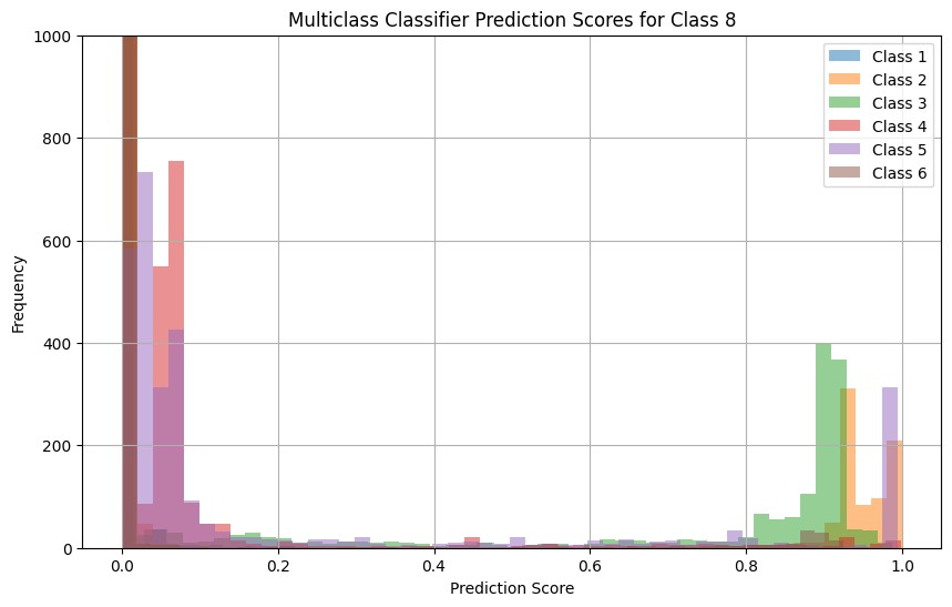
\includegraphics[width=0.9\textwidth]{Figure_7.png}
\caption{Escores de um classificador multiclasse treinado em seis classes, quando
apresentado às instâncias da classe 8 --- que ele nunca viu. Note a concentração de
massa próxima de $1{,}0$ para as classes 3, 2 e 5: o modelo não hesita, ele afirma com
convicção máxima que o hidrato é outra coisa. A restrição
$\sum_k \hat{p}_k = 1$ não lhe permite outra resposta. Adaptado de
\citet{Lopes2026PST}.}
\label{fig:closed-multiclasse}
\end{figure}

\begin{destaque}[O que a figura mostra e o que ela não mostra]
Ela não mostra um modelo mal treinado. Os picos próximos de $1{,}0$ indicam alta
confiança, e a alta confiança é apropriada \emph{dentro} do mundo fechado em que o
modelo foi treinado e avaliado.

O que a figura mostra é que a confiança de um classificador multiclasse não carrega
informação alguma sobre se a entrada pertence ao domínio para o qual ele foi treinado.
É um alerta que vale muito além do monitoramento de poços.
\end{destaque}

\begin{destaque}[Por que este é o resultado central da tese]
Um classificador multiclasse, no mesmo experimento, teria acertado $0\,\%$ --- não por
ser mal treinado, mas por construção. A restrição $\sum_k \hat{p}_k = 1$ o obriga a
distribuir toda a massa de probabilidade entre as seis classes que conhece. A resposta
``nenhuma delas'' não pertence ao seu espaço de saída.

Os $89\,\%$ não medem, portanto, uma melhoria incremental sobre uma linha de base: eles
medem a existência de uma capacidade que antes era literalmente inexpressável.
\end{destaque}

\subsection{Os onze por cento restantes}

Um resultado honesto exige olhar para o complemento. Onze por cento das instâncias de
hidrato foram atribuídas com confiança a alguma das seis classes conhecidas --- ou seja,
o sistema afirmou algo falso com convicção.

Em termos operacionais, esse é o modo de falha mais perigoso do sistema. Um alarme
ausente leva o operador a investigar por conta própria; um diagnóstico errado o leva a
investigar \emph{na direção errada}. O \cref{cap:operacao} retornará a essa distinção ao
discutir o projeto da interface.

\begin{destaque}[Uma comparação de escala]
Vale registrar a ordem de grandeza. Os $89\,\%$ deste experimento contrastam com os
$52\,\%$ obtidos sobre a anomalia de ICV no \cref{cap:mundoaberto} --- e a diferença é
instrutiva.

O hidrato tem assinatura física própria e distintiva. A falha de ICV é sintomaticamente
próxima de classes existentes. A capacidade de rejeição, portanto, não é uma propriedade
fixa do método: ela depende de quão distinta é a novidade em relação ao que já se
conhece. Sistemas de mundo aberto detectam melhor o que é mais estranho --- o que é
tranquilizador e, ao mesmo tempo, é a razão pela qual o número reportado em qualquer
trabalho da área deve vir acompanhado da identificação da classe escondida.
\end{destaque}

\section{O comprimento da janela}

\subsection{Um compromisso que não é técnico}

Quanto tempo de sinal é necessário para reconhecer um hidrato? Em uma janela causal,
$T$ define o histórico mínimo necessário após o início da aquisição; o atraso adicional
depende do passo entre janelas, do alinhamento do evento e da frequência de inferência.

A \cref{tab:closed-janelas} apresenta a varredura completa, de \SI{150}{\second} a
\SI{7500}{\second}, para o classificador binário de hidrato.

\begin{table}[htbp]
\centering
\caption{Desempenho do classificador binário de hidrato em função do comprimento da
janela $T$. FP e FN são as taxas de falso positivo e falso negativo.}
\label{tab:closed-janelas}
\small
\begin{tabular}{rcccccc}
\toprule
$\bm{T}$ \textbf{(s)} & \textbf{ACC} & \textbf{PR} & \textbf{REC} & $\bm{F_1}$ &
\textbf{FP} & \textbf{FN} \\
\midrule
150   & $0{,}866$ & $0{,}863$ & $0{,}898$ & $0{,}881$ & $0{,}175$ & $0{,}102$ \\
300   & $0{,}891$ & $0{,}883$ & $0{,}928$ & $0{,}905$ & $0{,}154$ & $0{,}072$ \\
600   & $0{,}891$ & $0{,}891$ & $0{,}918$ & $0{,}904$ & $0{,}144$ & $0{,}082$ \\
900   & $0{,}902$ & $0{,}885$ & $0{,}952$ & $0{,}917$ & $0{,}166$ & $0{,}048$ \\
1200  & $0{,}898$ & $0{,}893$ & $0{,}937$ & $0{,}915$ & $0{,}157$ & $0{,}063$ \\
1500  & $0{,}907$ & $0{,}911$ & $0{,}935$ & $0{,}923$ & $0{,}132$ & $0{,}065$ \\
2250  & $0{,}899$ & $0{,}923$ & $0{,}910$ & $0{,}917$ & $0{,}117$ & $0{,}090$ \\
3000  & $0{,}930$ & $0{,}949$ & $0{,}941$ & $0{,}945$ & $0{,}090$ & $0{,}059$ \\
3750  & $0{,}961$ & $0{,}958$ & $0{,}985$ & $0{,}971$ & $0{,}085$ & $0{,}015$ \\
4500  & $0{,}920$ & $0{,}895$ & $0{,}997$ & $0{,}943$ & $0{,}236$ & $\bm{0{,}003}$ \\
5250  & $0{,}962$ & $\bm{0{,}977}$ & $0{,}966$ & $0{,}971$ & $\bm{0{,}047}$ & $0{,}034$ \\
6000  & $0{,}869$ & $0{,}968$ & $0{,}832$ & $0{,}895$ & $0{,}056$ & $0{,}168$ \\
6750  & $0{,}942$ & $0{,}922$ & $\bm{1{,}000}$ & $0{,}959$ & $0{,}180$ & $\bm{0{,}000}$ \\
7500  & $\bm{0{,}966}$ & $0{,}958$ & $0{,}994$ & $\bm{0{,}975}$ & $0{,}092$ & $0{,}006$ \\
\bottomrule
\end{tabular}
\end{table}

\subsection{Três leituras da tabela}

\paragraph{A tendência.} A acurácia cresce de $0{,}866$ para $0{,}966$ ao longo de duas
ordens de grandeza de $T$. O ganho é real, mas modesto: dez pontos percentuais para um
aumento de cinquenta vezes no comprimento da janela. E ele não é monótono --- há uma
queda pronunciada em \SI{6000}{\second} ($0{,}869$), com revocação despencando para
$0{,}832$.

\begin{destaque}[Sobre a não monotonicidade]
A queda em \SI{6000}{\second} não deve ser explicada apressadamente. Duas causas
concorrem. Primeira, janelas mais longas produzem \emph{menos} exemplos de treinamento a
partir do mesmo conjunto de dados --- a variância da estimativa cresce. Segunda, com
$T = \SI{6000}{\second}$ a janela passa a conter, frequentemente, tanto o regime normal
quanto o evento inteiro, e o rótulo agregado torna-se ambíguo.

A lição metodológica: uma varredura de hiperparâmetro que produz curva ruidosa está
comunicando algo sobre a quantidade de dados, não apenas sobre o hiperparâmetro.
\end{destaque}

\paragraph{O compromisso entre FP e FN.} As duas últimas colunas revelam um padrão que a
acurácia esconde. Em \SI{4500}{\second}, a taxa de falso negativo cai para $0{,}003$ ---
praticamente nenhum hidrato escapa --- mas a de falso positivo sobe para $0{,}236$. Em
\SI{5250}{\second}, quase o oposto: FP de $0{,}047$ e FN de $0{,}034$.

Qual configuração é melhor? \textbf{A pergunta não tem resposta técnica.} Um hidrato não
detectado pode custar dias de produção e uma intervenção submarina; um alarme falso custa
atenção do operador. A razão entre esses custos é uma decisão da operadora, e o papel do
engenheiro é apresentar a curva, não escolher o ponto.

\paragraph{A leitura operacional.} É a mais importante, e a \cref{tab:closed-tempo} a
torna explícita.

\begin{table}[htbp]
\centering
\caption{Compromisso entre histórico mínimo e acurácia para três comprimentos de janela
representativos; o atraso efetivo depende do passo e do alinhamento.}
\label{tab:closed-tempo}
\begin{tabular}{rcc}
\toprule
$\bm{T}$ \textbf{(s)} & \textbf{Histórico mínimo} & \textbf{Acurácia} \\
\midrule
150  & $2{,}5$ minutos & $86{,}6\,\%$ \\
300  & $5$ minutos     & $89{,}1\,\%$ \\
900  & $15$ minutos    & $90{,}2\,\%$ \\
\bottomrule
\end{tabular}
\end{table}

\begin{resultadochave}
Reduzir a janela de \SI{900}{\second} para \SI{150}{\second} --- de quinze para dois
minutos e meio de histórico --- custa $3{,}6$ pontos percentuais de acurácia neste teste.
\end{resultadochave}

Esse número precisa ser confrontado, em cada implantação, com o intervalo disponível
para agir. A faixa de trinta minutos a cinco horas antes atribuída a
\citet{VARGAS2019} não foi confirmada na fonte consultada nesta revisão e, por isso, não
é usada aqui como evidência.

\begin{destaque}[A conclusão que inverte a intuição]
O gargalo do sistema não é o tempo de detecção. É a confiabilidade do diagnóstico.

Otimizar por latência, neste problema, é otimizar a variável errada. É por isso que o
restante deste livro investe em segmentação precisa (\cref{cap:segmentacao}), em
detecção de novidade confiável (\cref{cap:mahalanobis}) e em explicabilidade
(\cref{parte:explicabilidade}) --- e não em inferência mais rápida.
\end{destaque}

\section{Validação contra um modelo físico}

\subsection{A ideia}

Comparar um classificador com outro classificador diz pouco: ambos podem estar
compartilhando os mesmos vieses do conjunto de dados. Comparar um classificador com um
\textbf{modelo termodinâmico independente} é outra coisa --- o modelo físico não foi
treinado em dado nenhum e não conhece o 3W.

\subsection{O modelo de Motiee}

\begin{figure}[htbp]
\centering
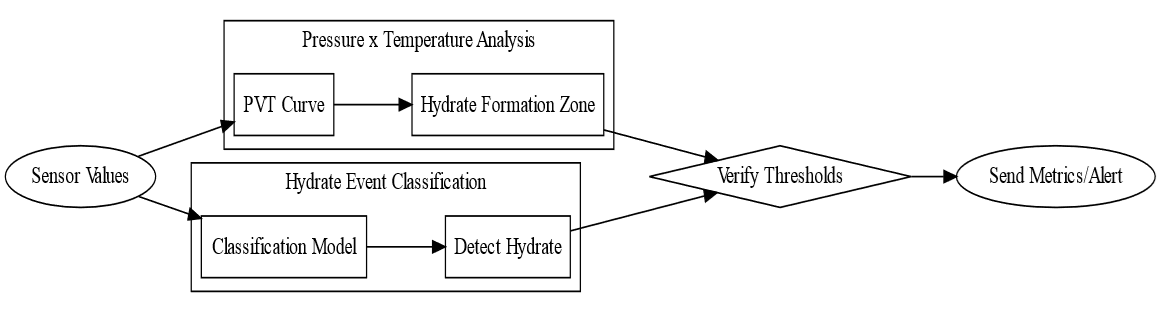
\includegraphics[width=\textwidth]{Figure_9.png}
\caption{Arquitetura de validação cruzada entre modelo físico e modelo aprendido. Os
mesmos valores de sensor alimentam dois caminhos independentes --- a análise
pressão--temperatura contra a envoltória de formação de hidrato e o classificador
binário --- cujos resultados são então confrontados antes de gerar o alerta. Adaptado de
\citet{Lopes2026PST}.}
\label{fig:closed-arquitetura}
\end{figure}

A correlação empírica de \citet[p.~98--99]{montie1991} estima a temperatura de formação
de hidrato $T_{\text{hid}}$ a partir da pressão absoluta $P$ e da densidade relativa do
gás $q$. Na forma publicada, define-se $x=\log_{10}(P/\mathrm{psia})$, e a saída é dada
em graus Fahrenheit:
\begin{equation}
\begin{split}
      T_{\text{hid},\,{}^\circ\mathrm{F}} = {} & -238{,}24469 + 78{,}99667\,x
            - 5{,}352544\,x^2 \\
      & + 349{,}473877\,q - 150{,}854675\,q^2 - 27{,}604065\,xq.
\end{split}
\label{eq:motiee}
\end{equation}
Trata-se de uma correlação de triagem para gás natural doce baseada em gravidade
específica, não de um modelo composicional. Por isso, seu uso fora da faixa de pressão e
composição coberta pela fonte exige validação contra dados de equilíbrio ou simulador
termodinâmico.

A partir dela define-se um índice de proximidade da condição de hidrato,
\begin{equation}
  C_{\text{hid}} = 100 \, \frac{T - T_{\text{hid}}}{T},
  \label{eq:chid}
\end{equation}
onde $T$ é a temperatura medida. Valores negativos ou próximos de zero indicam operação
dentro ou junto da envoltória de formação. A curva pressão--temperatura de referência é a
de \citet{Safamirzaei2015}.

\begin{figure}[htbp]
\centering
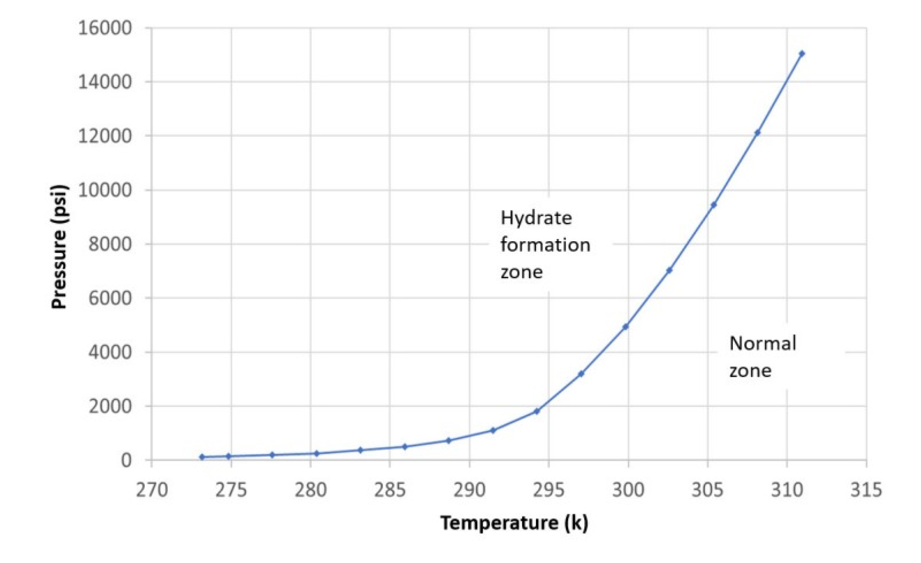
\includegraphics[width=0.92\textwidth]{figure_5.eps}
\caption{Envoltória de formação de hidrato no plano temperatura--pressão. A curva separa
a zona de operação normal da zona de formação: para uma dada pressão, temperaturas à
esquerda da curva colocam o sistema em risco. Adaptado de \citet{Lopes2026PST}.}
\label{fig:closed-envoltoria}
\end{figure}

A \cref{fig:closed-envoltoria} apresenta essa envoltória. Note que a curva é monotônica e
suave --- e é justamente essa simplicidade que a torna um instrumento de validação útil.
Ela não tem parâmetros ajustados aos dados, não conhece o 3W e não pode ter aprendido
nenhum atalho do conjunto. Se o classificador concorda com ela, a concordância significa
alguma coisa.

\begin{exemplo}{Usando a \cref{eq:motiee} na prática}
Considere um trecho de linha operando a $P = \SI{7}{\mega\pascal}$, ou aproximadamente
$1015\,\text{psia}$, com gás de densidade relativa $q = 0{,}65$ e temperatura medida
$T = \SI{18}{\celsius}$.

Com $x=\log_{10}(1015)\approx3{,}007$, a \cref{eq:motiee} fornece
$T_{\text{hid}}\approx60{,}4\,{}^\circ\mathrm{F}\approx\SI{15,8}{\celsius}$. Pela
\cref{eq:chid}, $C_{\text{hid}} \approx 100 \times (18 - 15{,}8)/18 \approx 12\,\%$.

Uma queda de aproximadamente $2{,}2$ graus na temperatura da linha levaria
$C_{\text{hid}}$ a zero. É esse tipo de raciocínio de margem que o modelo analítico
oferece e que um classificador, por si só, não comunica.
\end{exemplo}

\subsection{Resultado da comparação}

\begin{table}[htbp]
\centering
\caption{Classificador binário de hidrato \emph{versus} critério analítico baseado na
correlação de Motiee.}
\label{tab:closed-analitico}
\begin{tabular}{lcc}
\toprule
\textbf{Métrica} & \textbf{Classificador binário} & \textbf{Critério analítico} \\
\midrule
Acurácia            & $\bm{90{,}02\,\%}$ & $76{,}60\,\%$ \\
Falsos positivos    & $16{,}80\,\%$      & $18{,}61\,\%$ \\
Falsos negativos    & $\bm{4{,}80\,\%}$  & $20{,}10\,\%$ \\
\bottomrule
\end{tabular}
\end{table}

\begin{resultadochave}
O classificador supera o critério analítico em treze pontos percentuais de acurácia. A
diferença concentra-se nos falsos negativos: $4{,}8\,\%$ contra $20{,}1\,\%$ --- uma
redução de quatro vezes.
\end{resultadochave}

\subsection{Interpretando a diferença}

Por que o modelo físico perde? Não por estar errado. A correlação de Motiee descreve
corretamente a \emph{condição termodinâmica de formação} de hidrato. O que ela não
descreve é a \emph{cinética}: a formação leva tempo, depende da presença de água livre,
de nucleação, de histórico de escoamento e de eventual injeção de inibidor.

Um trecho pode estar dentro da envoltória por horas sem formar hidrato; outro pode formar
com margem aparentemente confortável, se houver acúmulo de água. O modelo analítico
responde ``é termodinamicamente possível?''; o classificador aprende a responder ``está
acontecendo?''.

\begin{destaque}[Complementaridade, não substituição]
As taxas de falso positivo são quase idênticas --- $16{,}8\,\%$ e $18{,}6\,\%$ --- o que
sugere que ambos os métodos são igualmente conservadores ao alertar. A diferença está
inteiramente na detecção.

A arquitetura sensata não escolhe entre os dois. O modelo analítico fornece contexto
físico interpretável --- a margem de $C_{\text{hid}}$ --- que o classificador não produz;
o classificador fornece a sensibilidade que o modelo não tem. O
\cref{cap:agente} retomará essa ideia em outro registro, ao alimentar o agente de
linguagem com conhecimento de domínio explícito.
\end{destaque}

Vale ainda notar que esta validação é possível apenas para o hidrato, porque apenas ele
dispõe de um modelo físico fechado e bem estabelecido. Para golfadas, incrustação ou
falha de ICV não há equivalente --- e essa é uma limitação da estratégia de validação,
não do classificador.

\subsection{A complementaridade na tela do operador}

\begin{figure}[htbp]
\centering
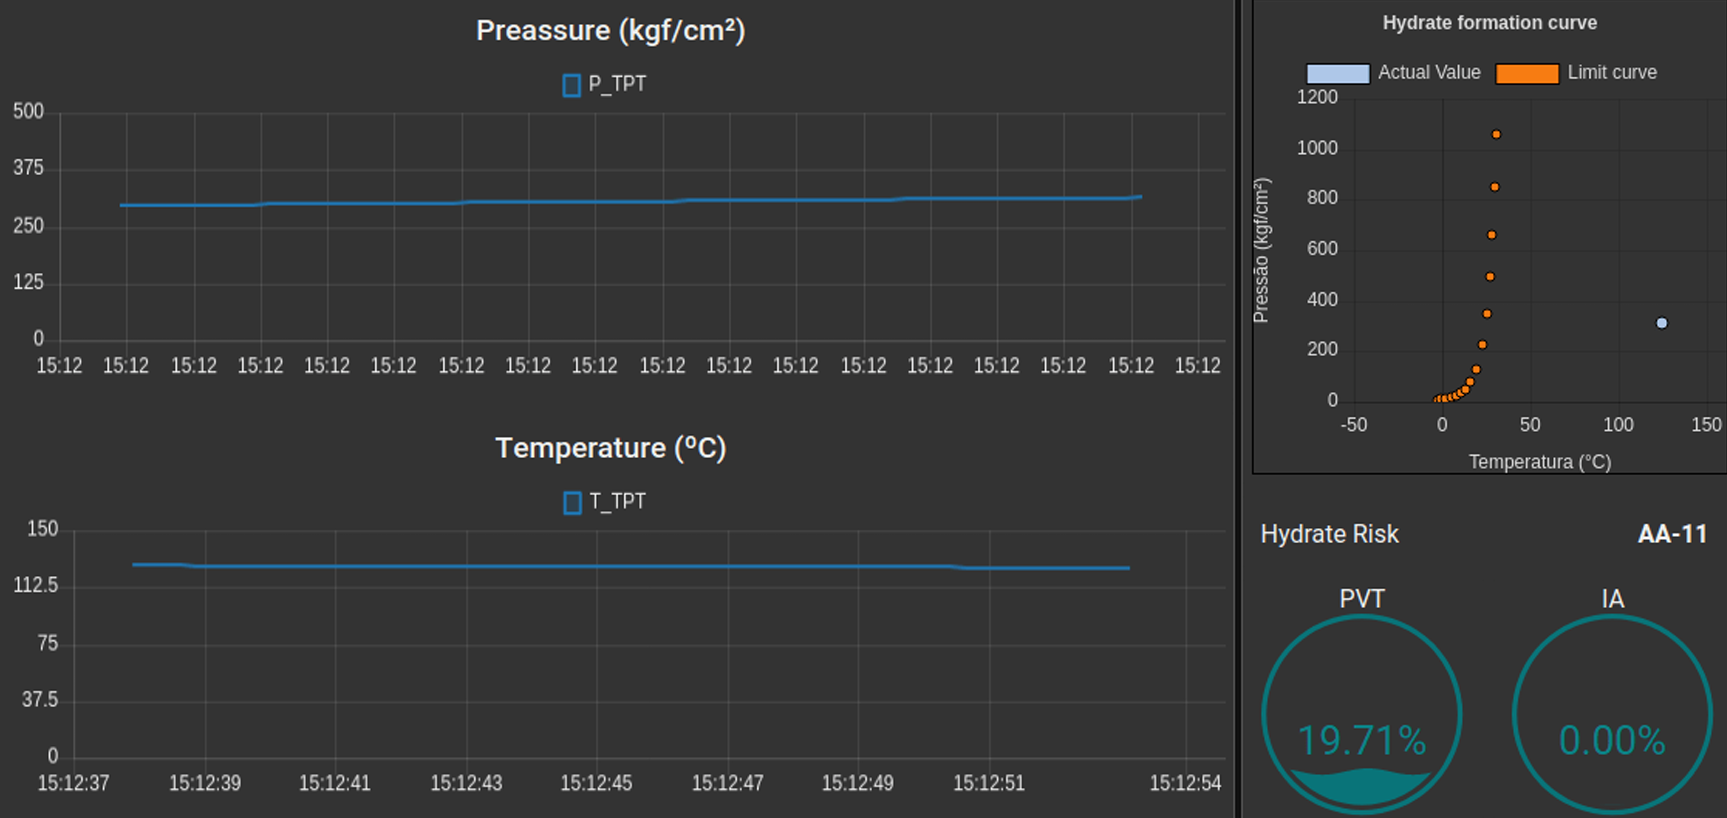
\includegraphics[width=\textwidth]{Figure_10.png}
\caption{Painel operacional com os dois indicadores lado a lado. À direita, a curva de
formação de hidrato com o ponto de operação atual; abaixo, os dois medidores de risco:
o analítico (PVT), em $19{,}71\,\%$, e o aprendido (IA), em $0{,}00\,\%$. Os dois números
respondem a perguntas diferentes e são apresentados sem tentativa de fundi-los em um só.
Adaptado de \citet{Lopes2026PST}.}
\label{fig:closed-painel}
\end{figure}

A \cref{fig:closed-painel} materializa a recomendação da seção anterior. A decisão de
projeto --- exibir os dois riscos separadamente, em vez de combiná-los em um índice
único --- é deliberada. Um risco analítico de $19{,}71\,\%$ com risco aprendido nulo
comunica ao operador algo específico e acionável: \emph{as condições termodinâmicas se
aproximam da envoltória, mas ainda não há assinatura de formação}. Um índice combinado
de, digamos, $10\,\%$ destruiria essa informação.

\begin{destaque}[Fundir indicadores é perder informação]
A tentação de reduzir múltiplos indicadores a um número único é forte, e quase sempre
equivocada em contextos de decisão especializada. Dois indicadores que discordam são
informativos precisamente por discordarem. O \cref{cap:operacao} desenvolverá esse
princípio ao discutir o projeto do painel do operador.
\end{destaque}

\section{Custo computacional}

O argumento recorrente contra ensembles é o custo. Convém quantificá-lo.

\begin{table}[htbp]
\centering
\caption{Custo computacional por inferência, para janela de \SI{900}{\second}.}
\label{tab:closed-custo}
\begin{tabular}{lcc}
\toprule
& \textbf{Memória} & \textbf{Latência} \\
\midrule
Um classificador binário   & $\approx \SI{2,3}{\mega\byte}$ & $\approx \SI{45}{\milli\second}$ \\
Ensemble de nove           & $\approx \SI{21}{\mega\byte}$  & $\approx \SI{405}{\milli\second}$ \\
\bottomrule
\end{tabular}
\end{table}

\begin{resultadochave}
O ensemble completo ocupa cerca de \SI{21}{\mega\byte} e responde em cerca de
\SI{405}{\milli\second} para uma janela de \SI{900}{\second}.
\end{resultadochave}

A inferência é mais de três ordens de grandeza menor que a janela avaliada. Cabe em um computador industrial
embarcado, e o custo de multiplicar por nove --- que parecia uma objeção séria no
\cref{cap:binarios} --- não é limitante no hardware e na frequência avaliados.

\begin{destaque}[Uma observação sobre argumentos de eficiência]
Este é um caso em que a quantificação delimita o debate. Objeções de custo computacional
devem ser sempre confrontadas com a escala de tempo do processo monitorado. Em
monitoramento de hidrato no cenário avaliado, a inferência é rápida em relação à janela;
rede, aquisição, concorrência entre poços e requisitos de disponibilidade ainda precisam
ser medidos na implantação.
\end{destaque}

\section{Limitações}

\begin{enumerate}[leftmargin=*,itemsep=0.4em]

\item \textbf{Uma única classe escondida.} O experimento foi feito removendo a classe 8.
Não se sabe se $89\,\%$ se sustentaria com outra classe --- e a comparação com os
$52\,\%$ da ICV no \cref{cap:mundoaberto} sugere fortemente que não.

\item \textbf{Detecção sem localização.} O sistema classifica a janela inteira. Não diz
onde, dentro dela, o evento começa. É a lacuna que o \cref{cap:segmentacao} preenche.

\item \textbf{Rejeição sem organização.} Rejeitar é o primeiro passo; o
\cref{cap:mundoaberto} mostrou o que vem depois, e mostrou também que essa etapa é a
mais frágil da cadeia.

\item \textbf{Rejeição sem explicação.} O sistema diz ``desconhecido'' sem dizer por quê.
É a \cref{parte:explicabilidade}.

\item \textbf{Validação física restrita ao hidrato.} As demais classes não dispõem de
modelo independente contra o qual comparar.

\end{enumerate}

\resumocapitulo{%
O experimento decisivo do princípio de mundo aberto consiste em treinar o ensemble sobre
seis classes, esconder completamente a classe 8 --- hidrato na produção --- e verificar
se suas instâncias são reconhecidas como desconhecidas: $89\,\%$ delas são, contra
$0\,\%$ que um classificador multiclasse obteria por construção. A varredura do
comprimento de janela, de \SI{150}{\second} a \SI{7500}{\second}, mostra ganho modesto e
não monótono ($0{,}866$ a $0{,}966$) e revela que reduzir a janela de quinze para dois
minutos e meio de histórico custa $3{,}6$ pontos percentuais; o atraso operacional ainda
depende do passo e do alinhamento. No ambiente avaliado, a inferência não é o gargalo.
A validação contra a correlação
termodinâmica de Motiee dá ao classificador $90{,}02\,\%$ de acurácia contra $76{,}60\,\%$
do critério analítico, com falsos negativos de $4{,}8\,\%$ contra $20{,}1\,\%$: o modelo
físico descreve a condição de formação, o classificador aprende a ocorrência. O custo do
ensemble --- \SI{21}{\mega\byte} e \SI{405}{\milli\second} --- é três ordens de grandeza
menor que a escala de tempo assumida para o processo e não foi limitante no ambiente
avaliado.}

\begin{exercicios}
\item Repita o experimento da classe escondida para cada uma das nove classes,
      reportando a taxa de rejeição em cada caso. Correlacione os resultados com alguma
      medida de distinção da assinatura --- por exemplo, a distância entre centroides no
      espaço latente. A hipótese de que ``a rejeição depende de quão estranha é a
      novidade'' se sustenta?

\item A \cref{tab:closed-janelas} mostra queda de acurácia em \SI{6000}{\second}.
      Projete dois experimentos que discriminem entre as duas explicações oferecidas
      (menos exemplos de treinamento \emph{versus} rótulo agregado ambíguo).

\item Para $T = \SI{4500}{\second}$, FP $= 0{,}236$ e FN $= 0{,}003$; para
      $T = \SI{5250}{\second}$, FP $= 0{,}047$ e FN $= 0{,}034$. Formule o problema de
      escolha como minimização de custo esperado, atribua custos plausíveis a um hidrato
      não detectado e a um alarme falso, e determine para que razão de custos cada
      configuração é preferível.

\item \textbf{Projeto de reprodução.} Com acesso às instâncias e às variáveis físicas
      necessárias, implemente a \cref{eq:motiee} e a \cref{eq:chid} para as classes 8 e
      9 do 3W e busque reproduzir a \cref{tab:closed-analitico}. Registre protocolo e
      divergências. Em seguida, examine os casos em que o critério analítico erra e o
      classificador acerta: há padrão?

\item O modelo analítico e o classificador têm taxas de falso positivo semelhantes mas
      taxas de falso negativo muito distintas. Proponha três formas de combiná-los ---
      conjunção, disjunção e voto ponderado --- e avalie cada uma quanto a FP, FN e
      interpretabilidade.

\item Estime o custo computacional do ensemble para os duzentos e cinquenta poços
      mencionados no \cref{cap:dual}, supondo inferência a cada \SI{60}{\second}. Discuta
      arquiteturas de implantação: inferência na plataforma, em terra, ou híbrida.

\item Argumente a favor e contra a seguinte afirmação: ``o resultado de $89\,\%$ é
      superestimado porque a classe 8 tem assinatura particularmente distintiva''. Que
      evidência adicional resolveria a disputa?
\end{exercicios}

\begin{leituras}
\item \citet{Lopes2026PST} --- o artigo que originou este capítulo.
\item \citet{LopesTese2025} --- a tese, para o contexto completo.
\item \citet{montie1991} e \citet{Safamirzaei2015} --- as correlações termodinâmicas
      usadas na validação independente.
\item \citet{VARGAS2019} --- a descrição do conjunto 3W.
\item \citet{Scheirer2013} --- a formalização do risco de espaço aberto, que dá suporte
      teórico ao experimento da classe escondida.
\end{leituras}

\chapter{Da detecção à segmentação}
\label{cap:segmentacao}

\begin{objetivos}
Ao final deste capítulo, você será capaz de:
\begin{itemize}[leftmargin=*,itemsep=0.2em]
  \item distinguir detecção de segmentação e justificar por que a segunda é
        operacionalmente superior;
  \item projetar uma U-Net unidimensional para segmentação de séries temporais;
  \item explicar o papel das conexões de atalho na preservação da resolução temporal;
  \item avaliar segmentação com IoU e com SoftED, e interpretar a diferença entre
        as duas famílias de métrica;
  \item diagnosticar desalinhamento de anotação a partir de padrões anômalos nas
        métricas.
\end{itemize}
\end{objetivos}

\section{A pergunta errada}

Todos os capítulos anteriores fizeram a mesma pergunta: \emph{esta janela contém uma
anomalia?} A resposta é um rótulo por janela.

Considere o que isso significa em operação. Com janelas de \SI{900}{\second}, o sistema
informa ``houve um evento em algum ponto destes quinze minutos''. O operador precisa
então examinar novecentas amostras para descobrir onde. Se a janela for de
\SI{7500}{\second}, são mais de duas horas de sinal.

A pergunta correta é outra: \emph{quais amostras, exatamente, pertencem ao evento?}

\begin{definicao}{Segmentação de séries temporais}
Tarefa de atribuir um rótulo a \emph{cada amostra} de uma série temporal, produzindo uma
saída de mesmo comprimento que a entrada. Formalmente, dado
$\mat{X} \in \R^{T \times S}$, produzir $\vect{y} \in \{0,1\}^{T}$, em contraste com a
detecção, que produz um único $y \in \{0,1\}$.
\end{definicao}

\begin{destaque}[Três ganhos, não um]
A mudança de detecção para segmentação parece um refinamento de granularidade. Ela é
mais que isso.

Primeiro, \textbf{localização}: o operador sabe onde olhar.

Segundo, \textbf{início do evento}: com o instante inicial identificado, torna-se
possível medir antecedência de detecção --- métrica que o rótulo por janela não permite
sequer definir.

Terceiro, e menos óbvio, \textbf{qualidade da entrada para as etapas seguintes}. Um
segmento delimitado com precisão contém apenas o evento; uma janela contém o evento mais
o regime normal que o precede. Todas as estat\'isticas calculadas sobre o segmento ---
e o \cref{cap:agente} calculará treze delas por sensor --- são tão boas quanto a
delimitação. \textbf{A segmentação é pré-requisito da explicabilidade.}
\end{destaque}

\section{A U-Net unidimensional}

\subsection{Por que esta arquitetura}

A U-Net foi proposta por \citet{Ronneberger2015} para segmentação de imagens médicas,
sob restrições que ecoam as deste problema: poucos exemplos anotados, necessidade de
saída na mesma resolução da entrada, e classes desbalanceadas.

Sua ideia central é o contorno de um dilema. Para reconhecer um evento é preciso
contexto amplo --- e contexto amplo se obtém reduzindo a resolução. Mas para delimitá-lo
com precisão é preciso resolução fina. As \termo{conexões de atalho}{skip connections}
resolvem o conflito transportando as ativações de alta resolução do codificador
diretamente para o decodificador, contornando o gargalo.

\subsection{Arquitetura}

\begin{center}
\small
\begin{tabular}{lll}
\toprule
\textbf{Bloco} & \textbf{Composição} & \textbf{Resolução} \\
\midrule
Entrada     & $(L, 1)$ & $L$ \\
Cod.\ 1     & Conv1D(32,5)+BN, $\times 2$; MaxPool(2); \ing{Dropout} $0{,}2$ & $L/2$ \\
Cod.\ 2     & Conv1D(64,5)+BN, $\times 2$; MaxPool(2); \ing{Dropout} $0{,}2$ & $L/4$ \\
Gargalo     & Conv1D(128,5)+BN, $\times 2$ & $L/4$ \\
Dec.\ 1     & \ing{UpSampling}(2); concatena atalho (64); Conv1D(64,5)+BN, $\times 2$ & $L/2$ \\
Dec.\ 2     & \ing{UpSampling}(2); concatena atalho (32); Conv1D(32,5)+BN, $\times 2$ & $L$ \\
Saída       & Conv1D(1,1), sigmoide & $L$ \\
\bottomrule
\end{tabular}
\end{center}

A saída é uma probabilidade por amostra, limiarizada em $0{,}5$. O modelo é aplicado
\textbf{por sensor}, e as regiões resultantes são combinadas em seguida --- decisão que
preserva a informação de \emph{qual} sensor evidencia o evento, e que será usada pelo
agente do \cref{cap:agente}.

\begin{destaque}[Por que núcleo 5 e não 3]
Com núcleos de tamanho 5, duas convoluções por bloco e dois níveis de subamostragem, o
campo receptivo do gargalo cobre algumas dezenas de amostras --- suficiente para
capturar a dinâmica de transição de um evento de poço, e ainda estreito o bastante para
que a fronteira do segmento não seja borrada. Com núcleos 3, o campo receptivo exigiria
mais níveis; com núcleos 7 ou maiores, as fronteiras perdem definição. É um compromisso
que vale a pena verificar empiricamente em qualquer aplicação nova.
\end{destaque}

\section{Protocolo experimental}

\begin{itemize}[leftmargin=*,itemsep=0.3em]
  \item \textbf{Dados}: 3W complementado por instâncias proprietárias de poços reais;
        quatro variáveis (P-PDG, P-TPT, T-TPT e P-MON-CKP).
  \item \textbf{Amostra}: 200 passos $\times$ 4 variáveis, ou 800 dimensões quando
        achatada.
  \item \textbf{Janela deslizante}: comprimento de 100 passos, passo de \SI{5}{\second}.
  \item \textbf{Pré-processamento}: imputação de faltantes (último válido, próximo
        válido, média), padronização e remoção de ruído por transformada
        \ing{wavelet}.
  \item \textbf{Validação}: cruzada estratificada em cinco dobras.
  \item \textbf{Treinamento}: Adam, 30 a 50 épocas.
  \item \textbf{Limiares}: $0{,}5$ na saída da U-Net; percentil 95 para a distância de
        Mahalanobis (\cref{cap:mahalanobis}); $0{,}3$ para os classificadores binários.
\end{itemize}

A avaliação é feita \textbf{poço a poço}, e não sobre um conjunto agregado. Dez poços
--- identificados como G1, A1, A2, A3, B1, C1, C2, D1, E1 e F1 --- são reportados
individualmente. Essa escolha é deliberada: o desvio padrão entre poços é a única
medida honesta de generalização disponível, e agregá-los produziria um número único que
esconderia exatamente a informação mais relevante.

\section{Resultados}

\subsection{Autoencoder \emph{versus} U-Net}

A \cref{tab:seg-comparacao} confronta a abordagem anterior --- detecção por erro de
reconstrução de autoencoder, como no \cref{cap:dual} --- com a segmentação por U-Net,
poço a poço.

\begin{table}[htbp]
\centering
\caption{Detecção por autoencoder \emph{versus} segmentação por U-Net, avaliadas no
nível de amostra, por poço.}
\label{tab:seg-comparacao}
\small
\begin{tabular}{lcccc}
\toprule
& \multicolumn{2}{c}{\textbf{Autoencoder}} & \multicolumn{2}{c}{\textbf{U-Net}} \\
\cmidrule(lr){2-3}\cmidrule(lr){4-5}
\textbf{Poço} & \textbf{ACC} & $\bm{F_1}$ & \textbf{ACC} & $\bm{F_1}$ \\
\midrule
G1 & $0{,}818$ & $0{,}706$ & $0{,}882$ & $0{,}731$ \\
A1 & $0{,}541$ & $0{,}703$ & $0{,}775$ & $0{,}739$ \\
A2 & $0{,}582$ & $0{,}736$ & $0{,}929$ & $0{,}936$ \\
A3 & $0{,}293$ & $0{,}454$ & $0{,}951$ & $0{,}915$ \\
B1 & $0{,}285$ & $0{,}443$ & $0{,}752$ & $0{,}632$ \\
C1 & $0{,}772$ & $0{,}766$ & $0{,}885$ & $0{,}817$ \\
C2 & $0{,}329$ & $0{,}277$ & $0{,}975$ & $0{,}912$ \\
D1 & $0{,}296$ & $0{,}457$ & $0{,}892$ & $0{,}777$ \\
E1 & $0{,}496$ & $0{,}663$ & $0{,}870$ & $0{,}874$ \\
F1 & $0{,}567$ & $0{,}724$ & $0{,}720$ & $0{,}674$ \\
\midrule
\textbf{Global} & $0{,}500 \pm 0{,}187$ & $0{,}593 \pm 0{,}160$ &
                  $\bm{0{,}863 \pm 0{,}082}$ & $\bm{0{,}801 \pm 0{,}102}$ \\
\bottomrule
\end{tabular}
\end{table}

\begin{resultadochave}
A acurácia média sobe de $0{,}500$ para $0{,}863$ --- e o desvio padrão entre poços cai
de $0{,}187$ para $0{,}082$, uma redução de $56\,\%$.
\end{resultadochave}

\subsection{O número que importa não é a média}

Uma acurácia de $0{,}500$ em um problema binário é o desempenho de uma moeda. É tentador
concluir que o autoencoder ``não funciona'', mas essa leitura é errada e vale
desmontá-la: o autoencoder do \cref{cap:dual} obteve $0{,}9894$ em operação real.

A diferença está na \emph{tarefa}. Lá ele decidia se uma janela era anômala; aqui, cada
amostra. O erro de reconstrução é um escalar por janela e não carrega informação
temporal fina; usá-lo para segmentar é usá-lo para o que ele não faz.

\begin{destaque}[A redução da variância é o resultado principal]
A média subiu $73\,\%$, mas é o desvio padrão que conta a história decisiva.

Com o autoencoder, a acurácia varia de $0{,}285$ (B1) a $0{,}818$ (G1) --- uma faixa de
cinquenta e três pontos percentuais. O sistema funciona bem em alguns poços e falha em
outros, e não há como saber de antemão em quais. \textbf{Um sistema imprevisível é
inutilizável, mesmo que sua média seja aceitável}, porque o operador não pode calibrar
quanta confiança depositar no alerta.

Com a U-Net, a faixa é de $0{,}720$ (F1) a $0{,}975$ (C2). O pior caso passa a ser
melhor que o caso médio anterior. É essa propriedade --- e não a média --- que torna o
sistema implantável.
\end{destaque}

Vale ainda notar o poço A3: acurácia de $0{,}293$ com o autoencoder e $0{,}951$ com a
U-Net, um ganho de sessenta e seis pontos percentuais. Esse poço reaparecerá adiante,
com um comportamento que revela algo sobre os dados, não sobre os modelos.

\subsection{Qualidade da delimitação}

Acurácia por amostra é uma métrica generosa em problemas desbalanceados. A
\cref{tab:seg-iou} acrescenta a interseção sobre união (\cref{eq:iou}), que mede
diretamente a sobreposição entre o segmento predito e o real.

\begin{table}[htbp]
\centering
\caption{Acurácia e interseção sobre união da segmentação por U-Net, por poço.}
\label{tab:seg-iou}
\small
\begin{tabular}{lcc}
\toprule
\textbf{Poço} & \textbf{ACC (\%)} & \textbf{IoU (\%)} \\
\midrule
A1 & $89{,}00$ & $74$ \\
A2 & $95{,}50$ & $93$ \\
A3 & $96{,}00$ & $85$ \\
B1 & $84{,}00$ & $56$ \\
C1 & $99{,}50$ & $98$ \\
C2 & $97{,}75$ & $84$ \\
D1 & $97{,}05$ & $93$ \\
E1 & $94{,}22$ & $83$ \\
F1 & $86{,}94$ & $72$ \\
G1 & $98{,}73$ & $94$ \\
\midrule
\textbf{Global} & $\bm{94{,}00}$ & $\bm{85}$ \\
\bottomrule
\end{tabular}
\end{table}

\begin{resultadochave}
IoU global de $85\,\%$: o segmento predito e o segmento real coincidem em cerca de cinco
sextos de sua união.
\end{resultadochave}

O poço B1 merece atenção: $84\,\%$ de acurácia mas apenas $56\,\%$ de IoU. A combinação é
diagnóstica --- o modelo acerta a maior parte das amostras, mas as fronteiras do
segmento estão substancialmente deslocadas. Em termos operacionais, o evento é detectado
e mal delimitado. Como toda a cadeia de explicabilidade depende da delimitação, esse é
um caso em que a saída deve ser marcada como de baixa confiança.

\section{Avaliação por SoftED}

\subsection{O problema das métricas ponto a ponto}

Considere um evento que começa na amostra 1000. Um detector o sinaliza na amostra 995;
outro, na 1400. Pela acurácia por amostra, ambos erram --- o primeiro erra cinco
amostras, o segundo quatrocentas. A diferença entre um sistema que antecipa em cinco
segundos e um que atrasa em quase sete minutos praticamente desaparece na métrica.

Em detecção de eventos, isso é inaceitável, e o SoftED de \citet{Salles2024softed}
existe para corrigi-lo, atribuindo crédito parcial a detecções próximas do instante
verdadeiro dentro de uma tolerância $k$.

\subsection{Resultados}

\begin{table}[htbp]
\centering
\caption{Avaliação SoftED com tolerância $k = 1000$ amostras, por poço.}
\label{tab:seg-softed}
\small
\begin{tabular}{lccc}
\toprule
\textbf{Poço} & \textbf{Precisão} & \textbf{Revocação} & $\bm{F_1}$ \\
\midrule
G1 & $1{,}00$ & $1{,}00$ & $1{,}00$ \\
A1 & $1{,}00$ & $1{,}00$ & $1{,}00$ \\
C2 & $1{,}00$ & $1{,}00$ & $1{,}00$ \\
D1 & $1{,}00$ & $1{,}00$ & $1{,}00$ \\
F1 & $1{,}00$ & $1{,}00$ & $1{,}00$ \\
B1 & $1{,}00$ & $0{,}40$ & $0{,}58$ \\
E1 & $1{,}00$ & $0{,}41$ & $0{,}58$ \\
A2 & $1{,}00$ & $0{,}30$ & $0{,}46$ \\
A3 & $0{,}00$ & $1{,}00$ & $0{,}00$ \\
\midrule
\textbf{Global} & $\bm{0{,}89}$ & $\bm{0{,}68}$ & $\bm{0{,}74}$ \\
\bottomrule
\end{tabular}
\end{table}

Métricas complementares globais: antecedência de detecção de $0{,}22$ e taxa de falso
positivo de $0{,}11$.

\subsection{Três leituras}

\paragraph{Precisão alta, revocação baixa.} Precisão de $0{,}89$ contra revocação de
$0{,}68$: quando o sistema aponta um evento, ele quase sempre está certo; mas ele deixa
passar cerca de um terço dos eventos. Para um sistema de alerta operacional, essa é a
assimetria preferível --- alarmes falsos destroem a confiança do operador mais
rapidamente do que eventos perdidos, que ainda podem ser capturados por outros meios.
Mas $0{,}68$ é um número que precisa melhorar.

\paragraph{Cinco poços perfeitos.} G1, A1, C2, D1 e F1 obtêm $1{,}00$ nas três métricas.
Metade dos poços é resolvida completamente. Isso indica que o método não tem uma
limitação intrínseca --- ele falha por razões específicas, em poços específicos, e essas
razões podem ser investigadas.

\paragraph{Antecedência de $0{,}22$.} O sistema raramente antecipa o evento; ele o
detecta no momento em que ocorre ou pouco depois. Para eventos de desenvolvimento lento
--- incrustação, aumento de BSW --- a antecipação seria valiosa e não está sendo obtida.

\subsection{O poço A3, ou como uma métrica revela um problema de dados}

O poço A3 apresenta a combinação mais estranha do livro:

\begin{center}
\small
\begin{tabular}{lc}
\toprule
Acurácia de segmentação (\cref{tab:seg-comparacao}) & $0{,}951$ \\
IoU (\cref{tab:seg-iou})                            & $85\,\%$ \\
SoftED --- revocação                                 & $1{,}00$ \\
SoftED --- precisão                                  & $\bm{0{,}00}$ \\
\bottomrule
\end{tabular}
\end{center}

Um modelo que segmenta com $95\,\%$ de acurácia e $85\,\%$ de IoU, e cuja precisão de
detecção de evento é exatamente zero. Isso não é um resultado ruim --- é um resultado
\emph{impossível}, sob a hipótese de que as anotações estão corretas.

\begin{destaque}[O que precisão $0{,}00$ com revocação $1{,}00$ significa]
Revocação $1{,}00$ indica que todo evento anotado tem uma detecção próxima. Precisão
$0{,}00$ indica que nenhuma detecção está próxima de um evento anotado. As duas
afirmações só são simultaneamente verdadeiras se houver \textbf{muitas} detecções, das
quais apenas algumas caem perto de eventos anotados --- ou se houver um deslocamento
sistemático maior que a tolerância entre o que o modelo detecta e o que está anotado.

A segunda hipótese é a mais provável, e ela aponta para \emph{desalinhamento da
anotação} do poço A3, não para falha do modelo. A alta acurácia de segmentação
corrobora: o modelo encontra consistentemente uma estrutura no sinal --- ela apenas não
está onde o rótulo diz.
\end{destaque}

Este é o tipo de achado que justifica reportar múltiplas métricas em vez de uma. Nenhuma
delas, isoladamente, revelaria o problema; a \emph{contradição} entre elas revela.

\section{Os classificadores binários sobre segmentos}

Com o segmento delimitado, os classificadores binários do \cref{cap:binarios} podem ser
aplicados a ele, e não à janela inteira. A arquitetura, mais leve por operar sobre um
segmento já isolado, é:

\begin{figure}[htbp]
\centering
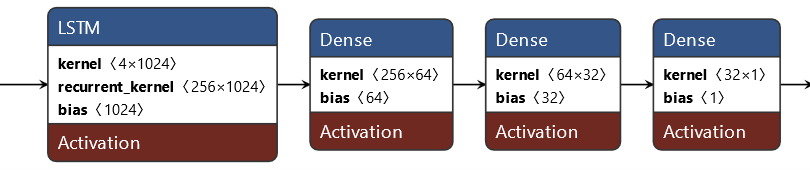
\includegraphics[width=\textwidth]{Figure_4.png}
\caption{Classificador binário aplicado ao segmento identificado, com as dimensões
efetivas de cada tensor de parâmetros: uma camada recorrente seguida de camadas densas
decrescentes até uma única saída escalar. A figura mostra a variante com LSTM de 256
unidades; o número de unidades recorrentes é ajustado por classe. Adaptado de
\citet{Lopes2026OTC}.}
\label{fig:seg-classificador}
\end{figure}

\begin{center}
\small
\begin{tabular}{ll}
\toprule
\textbf{Camada} & \textbf{Configuração} \\
\midrule
Entrada       & segmento \\
LSTM(128 a 256) & opcional, conforme a classe \\
Densa(64)     & + BN + \ing{Dropout} $0{,}3$ \\
Densa(32)     & + BN + \ing{Dropout} $0{,}2$ \\
Densa(16)     & + \ing{Dropout} $0{,}1$ \\
Densa(1)      & sigmoide \\
\bottomrule
\end{tabular}
\end{center}

O desempenho desses classificadores, e sobretudo o efeito do \emph{espaço} em que o
segmento é representado, é o assunto do \cref{cap:mahalanobis}.

\section{Limitações}

\begin{enumerate}[leftmargin=*,itemsep=0.4em]
  \item \textbf{Revocação de $0{,}68$}. Um terço dos eventos não é detectado dentro da
        tolerância.
  \item \textbf{Antecedência de $0{,}22$}. Praticamente não há detecção antecipada.
  \item \textbf{Variabilidade entre poços persistente}, ainda que reduzida: IoU de
        $56\,\%$ em B1 contra $98\,\%$ em C1.
  \item \textbf{Dependência da qualidade da anotação}, como o caso A3 demonstra de forma
        contundente.
  \item \textbf{Segmentação binária}. A U-Net separa normal de anômalo; ela não
        classifica o tipo de anomalia.
\end{enumerate}

\resumocapitulo{%
Trocar detecção por segmentação --- rótulo por amostra em vez de rótulo por janela ---
produz três ganhos: localização do evento, identificação do instante inicial e, o mais
importante para o restante do livro, qualidade das estatísticas que alimentarão a
camada de explicabilidade. A U-Net unidimensional, com codificador de dois níveis,
gargalo de 128 filtros e conexões de atalho que preservam a resolução temporal, eleva a
acurácia média de $0{,}500$ para $0{,}863$ e reduz o desvio padrão entre poços de
$0{,}187$ para $0{,}082$ --- é a redução de variância, mais que o ganho de média, que
torna o sistema implantável. A interseção sobre união global é de $85\,\%$. A avaliação
por SoftED, que atribui crédito parcial a detecções próximas do instante verdadeiro,
dá precisão de $0{,}89$, revocação de $0{,}68$ e medida $F_1$ de $0{,}74$, com cinco dos
dez poços resolvidos perfeitamente. O poço A3, com revocação $1{,}00$ e precisão
$0{,}00$ apesar de $95\,\%$ de acurácia de segmentação, revela desalinhamento de
anotação --- um achado que só a contradição entre métricas distintas torna visível.}

\begin{exercicios}
\item Calcule o campo receptivo do gargalo da U-Net descrita, considerando núcleos de
      tamanho 5, duas convoluções por bloco e dois níveis de subamostragem por fator 2.
      Compare com a duração típica da transição de um fechamento de DHSV.

\item Implemente a U-Net e reproduza a \cref{tab:seg-comparacao}. Em seguida, remova as
      conexões de atalho e repita. Quantifique a degradação em acurácia e, separadamente,
      em IoU. Qual das duas métricas é mais sensível à remoção? Por quê?

\item Um modelo obtém acurácia de $0{,}84$ e IoU de $0{,}56$ (poço B1). Construa um
      exemplo de segmentação predita e real, sobre uma série de mil amostras, compatível
      com esse par de valores. O que isso revela sobre o erro do modelo?

\item Implemente o SoftED e avalie a sensibilidade dos resultados à tolerância $k$. Trace
      precisão, revocação e $F_1$ globais em função de $k$, de 100 a 5000. Existe um
      valor de $k$ além do qual os resultados deixam de mudar? O que ele significa
      fisicamente?

\item O poço A3 apresenta precisão $0{,}00$ e revocação $1{,}00$. Projete um procedimento
      automático que detecte esse padrão de contradição entre métricas e sinalize
      possíveis erros de anotação em um conjunto de dados novo.

\item A antecedência de detecção é de $0{,}22$. Proponha três modificações da arquitetura
      ou do treinamento que poderiam aumentá-la --- por exemplo, ponderação assimétrica
      da perda nas amostras iniciais do evento --- e discuta o efeito esperado de cada
      uma sobre a taxa de falso positivo.

\item A U-Net é aplicada por sensor e as regiões são combinadas depois. Compare essa
      estratégia com uma U-Net multivariada que recebe os quatro sensores
      simultaneamente. Que informação cada abordagem preserva e qual descarta? Implemente
      ambas e compare.
\end{exercicios}

\begin{leituras}
\item \citet{Lopes2026OTC} --- o artigo que originou este capítulo.
\item \citet{Ronneberger2015} --- a U-Net original, cuja motivação em imagens médicas
      espelha as restrições do problema de poços.
\item \citet{Salles2024softed} --- a métrica SoftED e a discussão sobre por que métricas
      ponto a ponto são inadequadas para detecção de eventos.
\item \citet{VazVargas2026_3w2} --- a versão 2.0 do 3W, com discussão sobre a qualidade das
      anotações.
\end{leituras}

\chapter{Novidade no espaço latente}
\label{cap:mahalanobis}

\begin{objetivos}
Ao final deste capítulo, você será capaz de:
\begin{itemize}[leftmargin=*,itemsep=0.2em]
  \item aplicar a distância de Mahalanobis como escore de novidade e calibrar seu limiar
        por percentil;
  \item comparar espaços de representação --- bruto, latente de autoencoder e penúltima
        camada de classificador --- por índices internos de qualidade;
  \item explicar por que uma representação treinada para discriminar supera uma
        treinada para reconstruir, na tarefa de detectar o desconhecido;
  \item interpretar razões de separação entre classes conhecidas e desconhecidas;
  \item reconhecer as hipóteses estatísticas embutidas no método e as situações em que
        elas falham.
\end{itemize}
\end{objetivos}

\section{Retomando um resultado incômodo}

O \cref{cap:mundoaberto} apresentou um achado que ficou sem explicação: autoencoder,
VAE e DCN produziram acurácias de $0{,}730$, $0{,}727$ e $0{,}725$. Três arquiteturas de
sofisticação crescente, desempenho indistinguível.

A interpretação oferecida na ocasião foi que o gargalo estava em outro lugar. Este
capítulo mostra que a interpretação estava certa e localiza o gargalo com precisão: o
problema não é \emph{qual} autoencoder, mas o fato de usar um autoencoder.

\begin{destaque}[A hipótese deste capítulo]
Um autoencoder é treinado para minimizar erro de reconstrução. Nada em seu objetivo o
incentiva a \emph{separar} classes; ao contrário, ele gasta capacidade representando
fielmente aquilo que é comum a todas elas.

Um classificador multiclasse é treinado justamente para separar. A representação
implícita em sua penúltima camada --- o vetor que alimenta a camada de saída --- é,
por construção, um espaço em que as classes são linearmente separáveis.

A hipótese é que \textbf{esse espaço, construído para discriminar entre classes
conhecidas, também é melhor para reconhecer o desconhecido} --- mesmo que nada em seu
treinamento tenha visado a isso.
\end{destaque}

\section{A distância de Mahalanobis como escore}

\subsection{Definição}

Dado um conjunto de referência com média $\bm{\mu}$ e covariância $\mat{\Sigma}$, a
distância de Mahalanobis (\cref{eq:mahalanobis}) de um ponto $\vect{z}$ é
\[
  d_M(\vect{z}) = \sqrt{(\vect{z} - \bm{\mu})^\top \mat{\Sigma}^{-1} (\vect{z} - \bm{\mu})}.
\]

Sua virtude sobre a distância euclidiana é ponderar cada direção pela variabilidade
observada. Em um espaço latente onde algumas dimensões variam muito naturalmente e
outras quase nada, essa correção é o que separa um escore útil de um escore dominado
pelas direções de maior escala.

\subsection{Calibração do limiar}

O limiar é fixado no \textbf{percentil 95} da distribuição de $d_M$ sobre os dados
conhecidos. A escolha é operacional, não estatística: aceita-se, por construção, uma
taxa de falso alarme de aproximadamente $5\,\%$ em troca de sensibilidade.

\begin{destaque}[Por que percentil e não $\chi^2$]
Sob normalidade multivariada, $d_M^2$ segue distribuição $\chi^2$ com graus de liberdade
iguais à dimensão, e o limiar poderia ser lido diretamente de uma tabela.

Os dados não são normais. Calibrar por percentil empírico dispensa a hipótese e produz a
taxa de falso alarme desejada \emph{por construção}, qualquer que seja a distribuição
real. É um exemplo geral: quando a hipótese paramétrica é duvidosa e há dados
suficientes, o quantil empírico é preferível ao valor teórico.
\end{destaque}

\section{Três espaços em competição}

\begin{enumerate}[leftmargin=*,itemsep=0.4em]
  \item \textbf{Espaço bruto}, com $200 \times 4 = 800$ dimensões. Nenhuma transformação.
  \item \textbf{Latente de autoencoder LSTM}, com $128$ dimensões. Codificador:
        entrada $\to$ LSTM(256) $\to$ LSTM(128) $\to$ Densa(128). Decodificador
        simétrico. Treinado para reconstruir.
  \item \textbf{Penúltima camada de classificador multiclasse}, com $64$ dimensões.
        Treinada para discriminar entre as classes conhecidas.
\end{enumerate}

\begin{figure}[htbp]
\centering
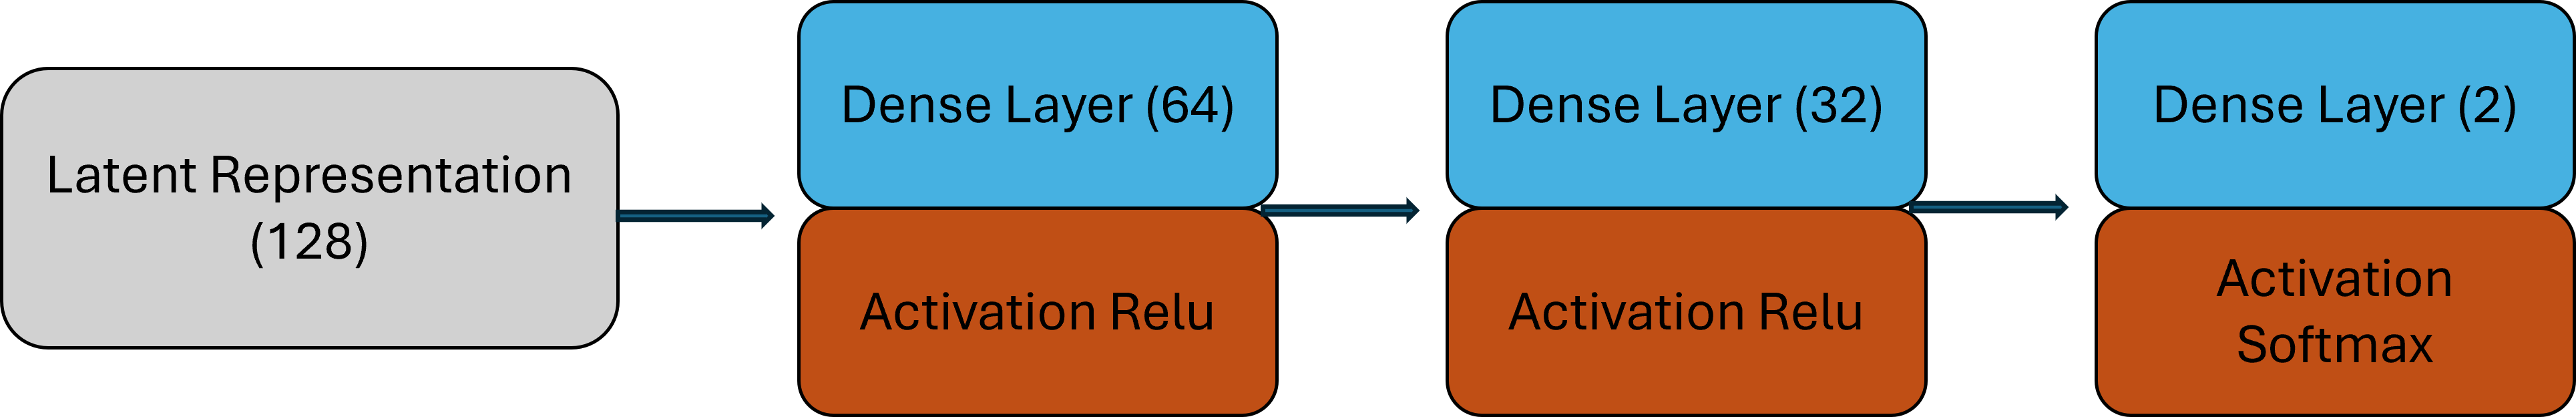
\includegraphics[width=\textwidth]{binary_classifiers.png}
\caption{Cabeça classificadora aplicada sobre a representação latente: duas camadas
densas com ativação ReLU seguidas da camada de saída. É a mesma cabeça para os três
espaços comparados, o que isola o efeito da representação.}
\label{fig:mahal-cabeca}
\end{figure}

O controle experimental importa: a arquitetura da cabeça classificadora é idêntica nos
três casos. Qualquer diferença de desempenho é atribuível à representação, não ao
classificador.

\section{Resultados}

\subsection{Detecção de novidade}

A \cref{tab:mahal-deteccao} apresenta o resultado central. Cada linha corresponde a uma
classe tratada como \emph{desconhecida} --- removida do treinamento --- e reporta a
fração de suas amostras corretamente identificadas como novidade por três métodos.

\begin{table}[htbp]
\centering
\caption{Acurácia de detecção de novidade (\%) por classe tratada como desconhecida,
sob três abordagens.}
\label{tab:mahal-deteccao}
\small
\begin{tabular}{lccc}
\toprule
\textbf{Classe tratada como desconhecida} & \textbf{Class.\ bin.} &
\textbf{Mahal.\ bruto} & \textbf{Mahal.\ latente} \\
\midrule
1 --- Aumento de BSW           & $22{,}8$ & $41{,}5$ & $\bm{99{,}0}$ \\
2 --- Fechamento de DHSV       & $76{,}9$ & $77{,}1$ & $\bm{96{,}5}$ \\
3 --- Golfadas severas         & $48{,}1$ & $61{,}0$ & $\bm{99{,}0}$ \\
4 --- Instabilidade de fluxo   & $44{,}7$ & $57{,}8$ & $\bm{96{,}0}$ \\
5 --- Perda rápida de produtiv.& $\bm{0{,}1}$ & $62{,}3$ & $67{,}5$ \\
6 --- Restrição rápida no PCK  & $47{,}6$ & $47{,}6$ & $\bm{99{,}0}$ \\
7 --- Incrustação no PCK       & $36{,}5$ & $36{,}7$ & $52{,}3$ \\
8 --- Hidrato na produção      & $50{,}5$ & $91{,}1$ & $\bm{99{,}0}$ \\
9 --- Hidrato no serviço       & $51{,}9$ & $88{,}7$ & $\bm{99{,}0}$ \\
Falha de ICV                   & $37{,}0$ & $67{,}5$ & $\bm{98{,}2}$ \\
\bottomrule
\end{tabular}
\end{table}

\begin{resultadochave}
Aplicar a distância de Mahalanobis no espaço latente do classificador multiclasse eleva
a detecção de novidade a $99\,\%$ em cinco das dez classes, e a mais de $96\,\%$ em sete
delas. Sobre a anomalia de ICV --- a única genuinamente inédita --- o salto é de
$52\,\%$ (\cref{cap:mundoaberto}) para $\bm{98{,}2\,\%}$.
\end{resultadochave}

\subsection{Três observações}

\paragraph{A progressão é sistemática.} Em nove das dez linhas, o Mahalanobis no espaço
bruto supera os classificadores binários, e o Mahalanobis latente supera o bruto. Não é
um ganho concentrado em casos favoráveis: é uma melhoria uniforme, o que é a assinatura
de uma mudança correta de método e não de ajuste ao conjunto de teste.

\paragraph{A classe 5 e o valor de $0{,}1\,\%$.} Um detector que identifica um décimo de
um por cento das novidades de uma classe está, para todos os efeitos, cego a ela. Ainda
assim, o Mahalanobis latente eleva o número a $67{,}5\,\%$ --- o pior resultado da
coluna, e um ganho de seiscentas vezes. A classe 5 continua sendo o ponto fraco do
sistema em todos os capítulos deste livro.

\paragraph{A classe 7 e o limite físico.} A incrustação no PCK atinge apenas $52{,}3\,\%$
mesmo no melhor espaço. A explicação é a escala temporal: incrustação se desenvolve ao
longo de semanas, e uma janela de duzentos passos não contém a evidência necessária.
Nenhuma escolha de representação corrige um problema de janela.

\subsection{Quanto o desconhecido se afasta}

A acurácia diz se o limiar foi ultrapassado. A \cref{tab:mahal-separacao} diz por quanto.

\begin{table}[htbp]
\centering
\caption{Razão de separação: distância de Mahalanobis média das amostras desconhecidas
dividida pela das conhecidas, nos espaços bruto e latente.}
\label{tab:mahal-separacao}
\small
\begin{tabular}{lcc}
\toprule
\textbf{Classe desconhecida} & \textbf{Espaço bruto} & \textbf{Espaço latente} \\
\midrule
1 & $2{,}1\times$ & $15{,}8\times$ \\
2 & $1{,}8\times$ & $12{,}4\times$ \\
3 & $2{,}3\times$ & $18{,}2\times$ \\
4 & $2{,}0\times$ & $16{,}1\times$ \\
5 & $1{,}9\times$ & $14{,}7\times$ \\
6 & $2{,}4\times$ & $13{,}9\times$ \\
8 & $<1{,}0\times$ & $\bm{186{,}5\times}$ \\
9 & $2{,}2\times$ & $17{,}3\times$ \\
\bottomrule
\end{tabular}
\end{table}

\begin{destaque}[A linha da classe 8]
No espaço bruto, a razão de separação da classe 8 é \emph{menor que um}: as amostras de
hidrato estão, em média, \textbf{mais próximas} do centro dos dados conhecidos do que as
próprias amostras conhecidas. Qualquer detector de novidade baseado em distância
falharia --- não por má calibração, mas porque no espaço bruto a informação simplesmente
não está disponível de forma acessível a uma métrica de distância.

No espaço latente, a mesma classe atinge $186{,}5\times$. É o maior valor da tabela por
uma ordem de grandeza.

A inversão é a demonstração mais forte da tese deste capítulo. Nenhum ajuste de limiar,
nenhuma escolha de escore, nenhuma sofisticação algorítmica recuperaria o desempenho no
espaço bruto. \textbf{A representação não é um detalhe de pré-processamento; ela
determina o que é detectável.}
\end{destaque}

Vale ainda notar a uniformidade das demais linhas: entre $12{,}4\times$ e $18{,}2\times$
no latente, contra $1{,}8\times$ a $2{,}4\times$ no bruto. O ganho é de aproximadamente
uma ordem de grandeza, de forma consistente.

\subsection{Por que o latente é melhor: a evidência direta}

Até aqui o argumento foi indireto --- o desempenho é melhor, logo o espaço é melhor. A
\cref{tab:mahal-qualidade} mede a qualidade dos espaços diretamente, pelos índices
internos do \cref{cap:novidades}.

\begin{table}[htbp]
\centering
\caption{Qualidade do espaço de representação segundo três índices internos. Para
silhueta e Calinski-Harabasz, maior é melhor; para Davies-Bouldin, menor é melhor.}
\label{tab:mahal-qualidade}
\small
\begin{tabular}{lcc}
\toprule
\textbf{Índice} & \textbf{Latente do autoencoder} & \textbf{Latente do multiclasse} \\
\midrule
Silhueta            & $-0{,}0149$   & $\bm{0{,}2299}$ \\
Calinski-Harabasz   & $687{,}8008$  & $\bm{2818{,}231}$ \\
Davies-Bouldin      & $4{,}5592$    & $\bm{1{,}746}$ \\
\bottomrule
\end{tabular}
\end{table}

\begin{resultadochave}
A silhueta do latente do autoencoder é \textbf{negativa} ($-0{,}0149$): em média, as
amostras estão mais próximas de um agrupamento vizinho do que do seu próprio. O latente
do multiclasse atinge $0{,}2299$. O índice Calinski-Harabasz é quatro vezes maior e o
Davies-Bouldin, dois pontos e meio menor.
\end{resultadochave}

\begin{destaque}[A explicação retroativa do \cref{cap:mundoaberto}]
Silhueta negativa significa que \textbf{não há estrutura de classe} no latente do
autoencoder. Isso explica, de uma vez, três observações anteriores:

por que autoencoder, VAE e DCN produziram desempenho equivalente --- todos otimizavam
reconstrução, e nenhum criava separação;

por que o agrupamento sobre o material rejeitado alcançou apenas $80{,}8\,\%$ --- não há
agrupamentos bem definidos para encontrar;

e por que o refinamento por limiar adaptativo precisou de tanta engenharia --- ele estava
compensando a ausência de estrutura no espaço subjacente.

O esforço do \cref{cap:mundoaberto} foi, em boa medida, gasto tentando extrair estrutura
de um espaço que não a tinha.
\end{destaque}

\subsection{Efeito sobre a classificação}

O ganho não se restringe à detecção de novidade. A \cref{tab:mahal-classificacao} mostra
o desempenho dos classificadores binários --- arquitetura idêntica --- sobre os três
espaços.

\begin{table}[htbp]
\centering
\caption{Desempenho dos classificadores binários em função do espaço de representação.
Média e desvio padrão sobre as classes.}
\label{tab:mahal-classificacao}
\small
\begin{tabular}{lcccc}
\toprule
\textbf{Espaço} & \textbf{ACC} & \textbf{PR} & \textbf{REC} & $\bm{F_1}$ \\
\midrule
Latente do multiclasse & $\bm{0{,}755} \pm 0{,}171$ & $\bm{0{,}732} \pm 0{,}280$ &
                          $\bm{0{,}685} \pm 0{,}384$ & $\bm{0{,}668} \pm 0{,}322$ \\
Latente do autoencoder & $0{,}697 \pm 0{,}154$ & $0{,}697 \pm 0{,}277$ &
                          $0{,}530 \pm 0{,}367$ & $0{,}559 \pm 0{,}318$ \\
Espaço bruto           & $0{,}691 \pm 0{,}162$ & $0{,}642 \pm 0{,}329$ &
                          $0{,}535 \pm 0{,}392$ & $0{,}543 \pm 0{,}349$ \\
\bottomrule
\end{tabular}
\end{table}

A ordem se mantém, mas as diferenças são bem menores --- seis pontos percentuais de
acurácia entre o melhor e o pior espaço, contra dezenas de pontos na detecção de
novidade.

\begin{destaque}[Uma assimetria reveladora]
A qualidade do espaço importa muito mais para \emph{detectar o desconhecido} do que para
\emph{classificar o conhecido}.

A razão é que um classificador suficientemente expressivo pode compensar uma
representação ruim: ele aprende a fronteira onde quer que ela esteja. Um escore de
distância não pode --- ele depende inteiramente da geometria que lhe é dada.

Corolário prático: se o objetivo é classificar bem o que se conhece, invista no
classificador. Se o objetivo é reconhecer o que não se conhece, invista na
representação.
\end{destaque}

Note também os desvios padrão elevados --- revocação de $0{,}685 \pm 0{,}384$. Um desvio
maior que metade da média indica que o desempenho varia enormemente entre classes, o que
as tabelas por classe dos capítulos anteriores já mostraram: excelente para as classes
2, 3 e 9, ruim para as classes 4 e 5.

\section{Balanço da evolução}

\begin{resultadochave}
No conjunto das classes avaliadas, a distância de Mahalanobis no espaço latente do
classificador multiclasse detecta $\bm{95{,}4\,\%}$ das falhas não vistas com
$\bm{4{,}5\,\%}$ de falsos alarmes --- uma melhoria média de $17\,\%$ sobre a melhor
alternativa anterior.
\end{resultadochave}

A \cref{tab:mahal-evolucao} resume o percurso da \cref{parte:evolucao}.

\begin{table}[htbp]
\centering
\caption{Evolução da detecção de novidade sobre a anomalia de ICV ao longo do livro.}
\label{tab:mahal-evolucao}
\small
\begin{tabular}{lll}
\toprule
\textbf{Capítulo} & \textbf{Método} & \textbf{Detecção} \\
\midrule
\cref{cap:dual}         & Erro de reconstrução, limiar $\mu + 3\sigma$ & apenas binária \\
\cref{cap:mundoaberto}  & Ensemble binário no latente do autoencoder   & $52{,}0\,\%$ \\
\cref{cap:mahalanobis}  & Mahalanobis no espaço bruto                  & $67{,}5\,\%$ \\
\cref{cap:mahalanobis}  & Mahalanobis no latente do multiclasse        & $\bm{98{,}2\,\%}$ \\
\bottomrule
\end{tabular}
\end{table}

\begin{destaque}[Uma lição sobre engenharia de sistemas de aprendizado]
A progressão de $52\,\%$ a $98{,}2\,\%$ não veio de um modelo maior, de mais dados ou de
uma arquitetura nova. Veio de duas mudanças conceituais: segmentar em vez de detectar
(\cref{cap:segmentacao}) e representar com um classificador em vez de um autoencoder
(este capítulo).

Ambas custam pouco em implementação. Ambas exigiram identificar corretamente onde estava
o gargalo --- e, no caso da representação, foi um resultado \emph{negativo} do
\cref{cap:mundoaberto} que apontou o caminho. Resultados negativos, quando reportados,
são informação.
\end{destaque}

\section{Limitações}

\begin{enumerate}[leftmargin=*,itemsep=0.4em]

\item \textbf{Hipótese elíptica.} A distância de Mahalanobis supõe distribuição
aproximadamente elíptica, caracterizada por média e covariância. Se a classe conhecida é
multimodal --- e várias são ---, a hipótese é violada e uma mistura de gaussianas ou uma
estimativa por vizinhança seria mais adequada.

\item \textbf{Ausência de tratamento de deriva.} $\bm{\mu}$ e $\mat{\Sigma}$ são
estimados uma vez. Poços mudam ao longo de anos, e o método não prevê atualização.

\item \textbf{Dependência da segmentação.} Todo o desempenho pressupõe segmentos bem
delimitados. Nos poços em que a U-Net vai mal --- B1, com IoU de $56\,\%$ ---, o escore
de novidade é calculado sobre um segmento contaminado.

\item \textbf{Variabilidade entre poços.} Persistente, como os desvios padrão da
\cref{tab:mahal-classificacao} mostram.

\item \textbf{Revocação e antecedência.} SoftED de $0{,}678$ e antecedência de $0{,}222$
permanecem inalteradas por este capítulo, que atua sobre a natureza da decisão e não
sobre o instante em que ela é tomada.

\item \textbf{Classes 5 e 7.} $67{,}5\,\%$ e $52{,}3\,\%$ mesmo no melhor espaço, por
razões que são de rótulo e de escala temporal, respectivamente.

\item \textbf{Ainda não há explicação.} O sistema agora detecta o desconhecido com
$98{,}2\,\%$ de acerto e continua incapaz de dizer uma palavra sobre o que ele é.

\end{enumerate}

\begin{destaque}[O que a \cref{parte:evolucao} deixa para a seguinte]
Ao final desta parte, o sistema sabe \emph{onde} está o evento, sabe \emph{que} ele é
desconhecido, e sabe com alta confiança. A única pergunta do \cref{cap:introducao} que
permanece inteiramente sem resposta é a terceira: \emph{por quê?}
\end{destaque}

\resumocapitulo{%
A distância de Mahalanobis aplicada ao espaço latente extraído da penúltima camada de um
classificador multiclasse detecta $95{,}4\,\%$ das falhas não vistas com $4{,}5\,\%$ de
falsos alarmes, contra $67{,}5\,\%$ no espaço bruto e $52\,\%$ com o ensemble sobre o
latente do autoencoder. Sobre a anomalia de ICV, a detecção salta de $52\,\%$ para
$98{,}2\,\%$. A razão é geométrica e mensurável: a silhueta do latente do autoencoder é
negativa ($-0{,}0149$), indicando ausência de estrutura de classe, enquanto a do
multiclasse é $0{,}2299$, com Calinski-Harabasz quatro vezes maior e Davies-Bouldin dois
pontos e meio menor. A razão de separação entre desconhecidos e conhecidos passa de
cerca de $2\times$ no bruto para $12$ a $18\times$ no latente, e atinge $186{,}5\times$
para a classe 8 --- que no espaço bruto tinha razão \emph{menor que um}. A qualidade da
representação importa muito mais para detectar o desconhecido do que para classificar o
conhecido: seis pontos percentuais de acurácia de classificação contra dezenas de pontos
de detecção de novidade. Isso explica retroativamente por que autoencoder, VAE e DCN
produziram desempenho indistinguível no \cref{cap:mundoaberto}. Permanecem em aberto as
classes 5 e 7, a antecedência de detecção e --- sobretudo --- a explicação.}

\begin{exercicios}
\item Demonstre que a distância de Mahalanobis é invariante a transformações lineares
      invertíveis do espaço, e que a distância euclidiana não é. Relacione esse fato à
      superioridade observada da primeira em espaços latentes com escalas heterogêneas.

\item A razão de separação da classe 8 é menor que $1{,}0$ no espaço bruto. Construa um
      exemplo bidimensional em que amostras de uma classe ausente do treinamento fiquem,
      em média, mais próximas do centroide dos dados de treinamento do que os próprios
      dados de treinamento. Que geometria produz esse efeito?

\item Implemente os três espaços e reproduza a \cref{tab:mahal-qualidade}. Em seguida,
      calcule a silhueta do latente de um classificador multiclasse treinado com
      diferentes números de classes ($3$, $5$, $7$, $9$). A qualidade do espaço melhora
      monotonicamente com o número de classes?

\item A hipótese elíptica é violada quando a classe conhecida é multimodal. Implemente
      uma alternativa baseada em mistura de gaussianas e compare com o Mahalanobis
      simples sobre as classes do 3W. Em quais classes o ganho é maior? Isso corresponde
      à sua expectativa sobre quais classes são multimodais?

\item O limiar é o percentil 95 dos dados conhecidos. Trace a curva de detecção de
      novidade \emph{versus} taxa de falso alarme variando o percentil de 80 a 99{,}9,
      para o espaço bruto e para o latente. Compare as áreas sob as curvas.

\item Argumenta-se que a classe 7 falha por razão de escala temporal e não de
      representação. Projete um experimento que teste essa hipótese --- por exemplo,
      repetindo a avaliação com janelas progressivamente maiores --- e preveja o
      resultado esperado sob a hipótese e sob sua negação.

\item Proponha um mecanismo de atualização de $\bm{\mu}$ e $\mat{\Sigma}$ que acompanhe
      a deriva lenta do poço sem absorver eventos anômalos. Discuta o compromisso entre
      taxa de adaptação e risco de o modelo aprender a considerar normal uma degradação
      progressiva.
\end{exercicios}

\begin{leituras}
\item \citet{Lopes2026OTC} --- o artigo que originou este capítulo.
\item \citet{Mahalanobis1936} --- o trabalho original que define a distância.
\item \citet{Rousseeuw1987}, \citet{Calinski1974} --- os índices internos usados na
      comparação de espaços.
\item \citet{Pimentel2014review} --- revisão de detecção de novidade, útil para situar o
      Mahalanobis entre as alternativas.
\item \citet{maaten2008visualizing} --- para a visualização dos espaços latentes, com as
      ressalvas já discutidas.
\end{leituras}


\part{A explicabilidade}\label{parte:explicabilidade}
\chapter{Modelos de linguagem como camada de raciocínio}
\label{cap:llm}

\begin{objetivos}
Este capítulo não ensina a construir um modelo de linguagem nem desenvolve a
arquitetura \ing{transformer} em detalhe; ele apresenta o mínimo necessário para
julgar o que essa tecnologia pode e não pode fazer no problema do livro. Ao final,
você será capaz de:
\begin{itemize}[leftmargin=*,itemsep=0.2em]
  \item enunciar a equação da atenção e explicar as duas propriedades que ela trouxe ---
        paralelização e caminho curto entre posições;
  \item explicar o que é uma mistura de especialistas e por que ela reduz o custo de
        inferência;
  \item reconhecer os elementos de um \ing{prompt} com saída estruturada e os critérios
        para validá-la;
  \item reconhecer os modos de falha característicos de modelos de linguagem ---
        alucinação, sensibilidade ao prompt, ausência de calibração --- e as
        salvaguardas correspondentes;
  \item posicionar corretamente o papel de um modelo de linguagem em um sistema de
        monitoramento industrial.
\end{itemize}
\end{objetivos}

\section{A pergunta que sobrou}

Ao final da \cref{parte:evolucao}, o sistema delimita o evento e, no experimento com a
anomalia de ICV, sinaliza corretamente $98{,}2\,\%$ de suas janelas como desconhecidas.
O que ele entrega ao operador é, literalmente, isto:

\begin{center}
\ttfamily
\{ segmento: [14230, 15870], classe: desconhecida, escore: 0.94 \}
\end{center}

O operador precisa então abrir as séries temporais, examinar cada sensor, comparar com o
regime anterior, lembrar de eventos semelhantes e formar uma hipótese. O sistema fez o
trabalho de percepção; todo o trabalho de \emph{interpretação} continua com o humano.

Esta parte do livro investiga se um modelo de linguagem pode assumir parte dessa carga.

\begin{destaque}[O que se está e o que não se está propondo]
\textbf{Não} se propõe substituir os modelos numéricos por um modelo de linguagem. Um
\ing{transformer} de propósito geral é ruim em séries temporais multivariadas
amostradas a cada segundo, e não há razão para esperar o contrário.

Propõe-se acrescentar uma camada \emph{acima} deles. Os modelos numéricos detectam,
segmentam e quantificam; o modelo de linguagem recebe as quantidades resultantes ---
não os dados brutos --- e produz a interpretação. É uma divisão de trabalho por
competência, e o restante desta parte a testa empiricamente.
\end{destaque}

\section{O \ing{transformer}}

\subsection{Atenção}

O mecanismo central, introduzido por \citet{Vaswani2017}, é a atenção por produto escalar
escalado (\cref{eq:atencao}):
\[
  \text{Atenção}(\mat{Q}, \mat{K}, \mat{V}) =
  \operatorname{softmax}\!\left( \frac{\mat{Q}\mat{K}^\top}{\sqrt{d_k}} \right) \mat{V}.
\]

A leitura intuitiva: cada posição da sequência emite uma \termo{consulta}{query}, compara-a
com as \termo{chaves}{keys} de todas as demais posições, e agrega os \termo{valores}{values}
ponderados pela similaridade. O resultado é que qualquer posição pode acessar qualquer
outra em uma única operação --- em contraste com uma LSTM, onde a informação precisa
atravessar todos os passos intermediários.

O fator $\sqrt{d_k}$ evita que o produto escalar cresça com a dimensão e sature a
\ing{softmax}.

\begin{destaque}[Por que isso mudou tudo]
Duas propriedades, e nenhuma delas é ``o modelo entende linguagem''.

\textbf{Paralelização.} Uma LSTM processa a sequência passo a passo, e o passo $t$ depende
do $t-1$. A atenção computa todas as posições simultaneamente. Isso é o que tornou
possível treinar sobre corpora de trilhões de tokens.

\textbf{Caminho curto.} Em uma LSTM, a distância informacional entre duas posições
separadas por $n$ passos é $O(n)$. Na atenção, é $O(1)$. Dependências de longo alcance
deixam de ser um problema arquitetural.
\end{destaque}

\subsection{Da arquitetura ao modelo de linguagem}

Empilhando blocos de atenção com camadas densas, normalização e conexões residuais, e
treinando o resultado para prever o próximo \termo{token}{token} em um corpus muito
grande, obtém-se um modelo de linguagem.

O que emerge desse treinamento --- e permanece objeto de debate legítimo --- é a
capacidade de executar tarefas não vistas explicitamente, quando descritas em linguagem
natural. É essa capacidade que este livro explora, com o ceticismo apropriado.

\section{Mistura de especialistas}

\begin{definicao}{Mistura de especialistas}
Arquitetura em que a camada densa de cada bloco é substituída por um conjunto de
sub-redes especialistas e uma rede de roteamento que seleciona, para cada
\ing{token}, apenas um subconjunto pequeno delas. O modelo tem muitos parâmetros no
total, mas ativa poucos por inferência.
\end{definicao}

O modelo usado nesta parte do livro tem aproximadamente \textbf{397 bilhões de parâmetros
totais} e ativa cerca de \textbf{17 bilhões} por \ing{token} --- uma fração de
aproximadamente $4\,\%$ \citep{Qwen35_2026}.

\begin{destaque}[Por que isso importa para uma aplicação industrial]
Um modelo denso de 397 bilhões de parâmetros exigiria muito mais memória e computação;
sua viabilidade dependeria de hardware, quantização, paralelismo e meta de latência. A
mistura de especialistas reduz o custo por \ing{token} ao ativar apenas parte dos
parâmetros.

Para o problema deste livro, a consequência prática é que a camada de linguagem pode ser
consultada em segundos, contra os \SI{405}{\milli\second} do ensemble numérico e os
segundos ou minutos de histórico das janelas numéricas. Na configuração observada, a
camada de raciocínio não dominou a latência; essa conclusão deve ser reavaliada sob carga
e com a latência de rede da implantação.
\end{destaque}

\section{Como se instrui um modelo de linguagem}

\subsection{Prompt}

\begin{definicao}{Prompt}
Texto de entrada fornecido ao modelo, contendo instruções, contexto, dados e formato de
saída desejado. Diferentemente de um programa, não é executado: é interpretado
estatisticamente.
\end{definicao}

A construção do prompt é a principal alavanca de engenharia disponível, e as decisões
relevantes para esta aplicação são quatro.

\begin{description}[leftmargin=0pt,style=nextline,itemsep=0.4em]

\item[Papel e escopo.] Declarar explicitamente o papel do modelo --- ``você é um
especialista em análise de dados de poços submarinos'' --- e, tão importante quanto,
seus limites --- ``julgue apenas com base nas estatísticas fornecidas''.

\item[Conhecimento de domínio explícito.] Não confiar no que o modelo possa ter
absorvido durante o pré-treinamento. Os perfis de classe do \cref{cap:agente} são
fornecidos no prompt, de forma explícita e verificável.

\item[Formato de saída estruturado.] Exigir JSON com campos definidos. Isso permite
validação automática e integração com o restante do sistema, e é o que separa um
experimento de uma peça de software.

\item[Temperatura baixa.] Reduzir a aleatoriedade da amostragem para privilegiar
consistência sobre criatividade.

\end{description}

\subsection{Saída estruturada}

O agente do \cref{cap:agente} produz, para cada segmento:

\begin{itemize}[leftmargin=*,itemsep=0.2em]
  \item três classes candidatas, ordenadas;
  \item uma justificativa por candidata, referenciando as estatísticas;
  \item um nível de confiança (\ing{High}, \ing{Medium}, \ing{Low});
  \item um nome e uma descrição, caso julgue tratar-se de fenômeno não catalogado.
\end{itemize}

\begin{destaque}[Por que três candidatas e não uma]
Porque uma única resposta força o modelo a comprometer-se, e um modelo que se compromete
sob incerteza produz afirmações confiantes e falsas --- exatamente a patologia que a
\cref{fig:closed-multiclasse} exibiu para o classificador multiclasse.

Três candidatas ordenadas comunicam a estrutura da incerteza. E, como o
\cref{cap:resultados-agente} mostrará, a diferença entre acerto na primeira escolha
($35{,}1\,\%$) e nas três primeiras ($63{,}9\,\%$) é grande o bastante para que essa
decisão de projeto seja o que separa um sistema inútil de um sistema útil.
\end{destaque}

\subsection{Modo de raciocínio}

Modelos recentes podem ser instruídos a gerar uma cadeia de raciocínio intermediária
antes da resposta final. O ganho, em tarefas que exigem comparação de múltiplas
evidências, é consistente; o custo é latência e \ing{tokens}.

Neste trabalho o modo está ativado, com temperatura $0{,}2$, \ing{top-p} $0{,}7$ e limite
de \num{4096} \ing{tokens}.

\begin{destaque}[Cadeia de raciocínio não é explicação]
Distinção importante e frequentemente ignorada. O texto que o modelo gera antes da
resposta é uma sequência que aumenta a probabilidade de acerto; não há garantia de que
ele descreva o processo computacional efetivamente realizado.

Neste sistema, a explicabilidade genuína vem de outro lugar: as estatísticas do
\cref{cap:agente} são calculadas deterministicamente e podem ser verificadas
independentemente. A justificativa do modelo é auditável \emph{contra elas}. É essa
ancoragem --- e não a cadeia de raciocínio --- que torna a saída confiável.
\end{destaque}

\section{Modos de falha}

Um capítulo sobre modelos de linguagem em contexto industrial que não enumere seus modos
de falha seria irresponsável.

\begin{description}[leftmargin=0pt,style=nextline,itemsep=0.5em]

\item[Alucinação.] O modelo produz afirmações plausíveis e falsas com a mesma fluência
com que produz afirmações corretas. Em um contexto onde a saída pode motivar uma
intervenção de milhões de dólares, isso é inaceitável sem salvaguarda.

\emph{Mitigação adotada}: fornecer todas as estatísticas no prompt, restringir a
julgamento sobre elas, exigir justificativa que as referencie, e manter o humano como
decisor.

\item[Sensibilidade ao prompt.] Reformulações semanticamente equivalentes podem alterar
o resultado. Isso compromete a reprodutibilidade.

\emph{Mitigação adotada}: prompt fixo, versionado e reportado integralmente.

\item[Ausência de calibração.] A confiança declarada pelo modelo não corresponde
necessariamente a uma probabilidade. ``High'' não significa $90\,\%$.

\emph{Mitigação adotada}: tratar o nível de confiança como ordinal e reportar a acurácia
empírica separadamente.

\item[Contaminação de dados.] O 3W é público desde 2019, e um modelo treinado em corpus
amplo pode tê-lo visto. Um acerto pode refletir memorização, não raciocínio.

\emph{Mitigação adotada}: nenhuma completamente satisfatória. É uma limitação declarada,
e o \cref{cap:resultados-agente} argumenta a partir dos \emph{padrões} de erro, que
memorização não explicaria bem.

\item[Custo e dependência externa.] Inferência em serviço de terceiros implica custo por
chamada, latência de rede e dependência operacional.

\emph{Mitigação adotada}: acionar o modelo apenas sobre segmentos já detectados como
anômalos --- um punhado por dia, não a cada segundo.

\end{description}

\begin{destaque}[A regra que organiza esta parte do livro]
Um modelo de linguagem \textbf{nunca decide sozinho} em um sistema de monitoramento
industrial. Ele propõe, justifica e ordena hipóteses. A decisão é do operador, e o
sistema deve ser projetado para que essa fronteira seja explícita na interface.
\end{destaque}

\section{Infraestrutura}

O modelo é acessado por um serviço gerenciado de inferência, com os parâmetros
resumidos na \cref{tab:llm-config}.

\begin{table}[htbp]
\centering
\caption{Configuração de inferência do agente.}
\label{tab:llm-config}
\small
\begin{tabular}{ll}
\toprule
\textbf{Parâmetro} & \textbf{Valor} \\
\midrule
Modelo                 & Qwen3.5-397B-A17B (mistura de especialistas) \\
Parâmetros totais      & $\approx 397$ bilhões \\
Parâmetros ativos      & $\approx 17$ bilhões por \ing{token} \\
Serviço                & NVIDIA NIM \\
Modo de raciocínio     & ativado \\
Temperatura            & $0{,}2$ \\
\ing{Top-p}            & $0{,}7$ \\
Limite de \ing{tokens} & \num{4096} \\
Formato de saída       & JSON estruturado \\
\bottomrule
\end{tabular}
\end{table}

\begin{destaque}[Sobre reprodutibilidade]
Modelos servidos por API são atualizados sem aviso, e o mesmo prompt pode produzir saídas
diferentes meses depois. Trabalhos que dependem deles devem reportar data de execução,
identificador exato do modelo e todos os parâmetros de amostragem --- e ainda assim a
reprodutibilidade é inferior à de um modelo local. É um custo real da abordagem, e o
\cref{cap:futuro} discutirá alternativas.
\end{destaque}

\resumocapitulo{%
Modelos de linguagem baseados em \ing{transformer} devem sua eficácia a duas propriedades
do mecanismo de atenção --- paralelização completa e caminho informacional de comprimento
constante entre quaisquer posições --- e não a qualquer compreensão no sentido humano. A
arquitetura de mistura de especialistas permite modelos de centenas de bilhões de
parâmetros com custo de inferência de modelos muito menores: o modelo aqui utilizado tem
$397$ bilhões de parâmetros e ativa $17$ bilhões por \ing{token}. A instrução se dá por
prompt, cujas decisões de projeto relevantes são declarar papel e escopo, fornecer
conhecimento de domínio explicitamente, exigir saída estruturada em JSON e usar
temperatura baixa. O agente produz três candidatas ordenadas, com justificativa e
confiança por candidata --- decisão que se mostrará determinante nos resultados. Os modos
de falha característicos são alucinação, sensibilidade ao prompt, ausência de calibração,
contaminação de dados de treinamento e dependência de serviço externo; cada um exige
salvaguarda explícita. A regra que organiza esta parte: o modelo de linguagem propõe e
justifica, nunca decide.}

\begin{exercicios}
\item Calcule a complexidade computacional da atenção em função do comprimento da
      sequência $n$ e da dimensão $d$. Compare com a de uma LSTM. Para que valores de $n$
      a atenção deixa de ser vantajosa?

\item Um modelo com $397$ bilhões de parâmetros ativa $17$ bilhões por \ing{token}.
      Estime a memória necessária para armazenar os pesos em precisão de 16 bits e a
      necessária para uma inferência. Discuta as implicações para implantação local em
      uma unidade de produção.

\item \textbf{Atividade com serviço externo.} Escreva um prompt que instrua um modelo a
      classificar um segmento anômalo de poço a partir de estatísticas fornecidas, com
      saída em JSON validável. Registre modelo, revisão, data e parâmetros; aplique-o a
      três segmentos e avalie a estabilidade das respostas ao reformular o prompt sem
      alterar seu conteúdo semântico.

\item Discuta a afirmação: ``a cadeia de raciocínio gerada pelo modelo é uma explicação
      de sua decisão''. Apresente um argumento contra e proponha um experimento que
      distinga entre cadeia de raciocínio fiel e cadeia de raciocínio confabulada.

\item Projete um procedimento automático de validação da saída do agente contra as
      estatísticas fornecidas no prompt --- por exemplo, verificar se cada afirmação
      numérica na justificativa corresponde a um valor efetivamente presente na entrada.
      Que fração das alucinações esse procedimento capturaria?

\item O 3W é público desde 2019 e pode ter sido visto durante o pré-treinamento. Proponha
      três estratégias para estimar o grau de contaminação e discuta os limites de cada
      uma.

\item Compare o custo total de propriedade de três arquiteturas: modelo servido por API,
      modelo aberto executado localmente, e modelo aberto ajustado ao domínio. Considere
      custo por inferência, latência, reprodutibilidade, privacidade dos dados e esforço
      de manutenção.
\end{exercicios}

\begin{leituras}
\item \citet{Vaswani2017} --- o artigo que introduz o \ing{transformer}.
\item \citet{Qwen2025} --- os fundamentos da família Qwen3; \citet{Qwen35_2026} --- a
      ficha oficial da versão Qwen3.5-397B-A17B utilizada nos experimentos.
\item \citet{Lopes2026LLM} --- o trabalho que originou esta parte do livro.
\item \citet{Liu2024oilgasLLM} e \citet{Chebbi2025energygpt} --- aplicações de modelos de
      linguagem no setor de petróleo e gás.
\item \citet{Sharma2025xaiagents} --- explicabilidade em sistemas baseados em agentes.
\item \citet{Zhang2025LLMTSFD} --- modelos de linguagem aplicados a detecção de falhas em
      séries temporais.
\end{leituras}

\chapter{A camada de agente}
\label{cap:agente}

\begin{objetivos}
Ao final deste capítulo, você será capaz de:
\begin{itemize}[leftmargin=*,itemsep=0.2em]
  \item descrever uma cadeia de pré-processamento que produza sinais comparáveis entre
        poços;
  \item calcular as treze métricas por sensor que traduzem um segmento anômalo em
        descrição quantitativa;
  \item descrever a construção de perfis estatísticos de classe robustos a valores
        extremos;
  \item reconhecer a estrutura do \ing{prompt} de um agente de diagnóstico e os
        critérios de validação de sua saída;
  \item explicar por que a tradução para linguagem intermediária é o que torna a camada
        de linguagem viável.
\end{itemize}
\end{objetivos}

\section{O problema de tradução}

Um modelo de linguagem não recebe séries temporais. Ele recebe texto.

A questão central deste capítulo é, portanto, uma questão de tradução: como converter um
segmento anômalo --- centenas de amostras, quatro sensores --- em uma descrição textual
que preserve a informação diagnóstica e seja compreensível pelo modelo.

Duas abordagens ingênuas falham de imediato. Despejar os números brutos no prompt gasta
milhares de \ing{tokens} em informação de baixíssima densidade, e o modelo não é bom em
extrair padrões de listas longas de floats. Descrever qualitativamente --- ``a pressão
subiu'' --- perde a magnitude, a velocidade e a relação entre sensores.

\begin{destaque}[A solução: uma linguagem intermediária]
Calcular deterministicamente um conjunto pequeno de métricas interpretáveis, e apresentar
ao modelo essas métricas em vez dos dados.

A escolha tem três consequências que valem ser explicitadas.

\textbf{Auditabilidade.} As métricas são calculadas por código verificável. Qualquer
afirmação do modelo pode ser confrontada com elas.

\textbf{Economia.} Treze números por sensor, contra centenas de amostras.

\textbf{Transferência de responsabilidade.} O trabalho de percepção fica com os métodos
numéricos --- que são bons nisso --- e o de interpretação com o modelo de linguagem.

O preço é que \emph{o que as métricas não capturam está perdido}. A escolha das métricas
é, portanto, a decisão de projeto mais consequente desta parte do livro.
\end{destaque}

\section{Pré-processamento}

A cadeia tem quatro etapas, nesta ordem.

\begin{enumerate}[leftmargin=*,itemsep=0.4em]

\item \textbf{Padronização por escore-$z$.} Cada sensor é centrado e escalado pela média
e pelo desvio padrão de sua referência. O conjunto usado para ajustar esses parâmetros
deve ser registrado para impedir vazamento e definir o que significa ``regime normal''.

\item \textbf{Normalização Min-Max para $[0,1]$.} Acomoda a entrada ao intervalo usado
pelo restante da cadeia. Se seus limites forem ajustados sobre as mesmas amostras da
etapa anterior, a composição é equivalente à normalização Min-Max direta; para ter
efeito adicional, as duas etapas precisam usar referências de ajuste distintas e
exclusivas do treinamento.

\item \textbf{Remoção de ruído por \ing{wavelet}.} Transformada de Daubechies db4, nível
3, com limiarização suave.

\item \textbf{Tratamento de valores ausentes.} Conforme o \cref{cap:dados}.

\end{enumerate}

\begin{destaque}[Por que db4, nível 3, limiar suave]
A escolha não é arbitrária, e cada componente responde a uma exigência do problema.

\textbf{Daubechies 4} tem suporte compacto e quatro momentos nulos --- suficiente para
representar bem transições abruptas, como o fechamento de uma válvula, sem introduzir os
artefatos oscilatórios que uma base mais suave produziria.

\textbf{Nível 3} remove três oitavas de alta frequência. Em sinais amostrados a cada
segundo, isso elimina ruído de instrumentação preservando dinâmicas de dezenas de
segundos.

\textbf{Limiarização suave} encolhe os coeficientes em vez de zerá-los, evitando as
descontinuidades que a limiarização dura introduz --- descontinuidades que seriam
interpretadas pelas métricas de \texttt{slope} e \texttt{rate} como eventos reais.
\end{destaque}

\subsection{Seleção de instâncias}

Uma decisão metodológica com consequência direta sobre a interpretação dos resultados:

\begin{itemize}[leftmargin=*,itemsep=0.3em]
  \item usam-se \textbf{apenas instâncias de poços reais} (\texttt{WELL});
  \item instâncias simuladas são acrescentadas somente quando uma classe tem menos de
        trinta instâncias reais;
  \item instâncias desenhadas à mão (\texttt{DRAWN}) são \textbf{sempre excluídas}.
\end{itemize}

A justificativa: o objetivo é avaliar a capacidade de interpretar fenômenos físicos
reais. Uma instância desenhada à mão contém a assinatura que um especialista
\emph{acredita} que o evento tem --- e um acerto sobre ela mediria concordância com a
intuição do anotador, não com a física.

\section{As treze métricas}

Para cada sensor, comparam-se dois trechos: o \termo{regime de base}{baseline}, anterior
ao evento, e o \termo{regime do evento}{event window}, delimitado pela segmentação do
\cref{cap:segmentacao}. Sejam $\bar{b}$ e $\sigma_b$ a média e o desvio padrão do
primeiro, e $\bar{e}$ e $\sigma_e$ os do segundo.

\subsection{Métricas de deslocamento}

\begin{align}
  \delta &= \bar{e} - \bar{b}, \label{eq:ag-delta} \\
  \text{variação percentual} &= 100 \, \frac{\delta}{|\bar{b}|}, \label{eq:ag-pct} \\
  z &= \frac{|\delta|}{\max(\sigma_b, 10^{-6})}. \label{eq:ag-z}
\end{align}

\begin{destaque}[As três métricas dizem coisas diferentes]
Uma pressão que sobe \SI{5}{\bar} sobre uma base de \SI{200}{\bar} com desvio padrão de
\SI{0,5}{\bar} tem $\delta = 5$, variação percentual de $2{,}5\,\%$ e $z = 10$.

O deslocamento absoluto é pequeno. A variação percentual é desprezível. E o escore-$z$
de $10$ indica um evento estatisticamente extraordinário.

É por isso que as três são fornecidas ao modelo. Cada uma responde a uma pergunta:
``quanto mudou?'', ``mudou muito em relação ao nível?'' e ``mudou muito em relação ao
que costuma variar?''. A última é quase sempre a diagnóstica, e é a que um humano
examinando o gráfico tende a subestimar.

O termo $\max(\sigma_b, 10^{-6})$ protege contra divisão por zero quando o sensor está
congelado --- situação frequente, como o \cref{cap:dados} discutiu.
\end{destaque}

\subsection{Métricas categóricas}

Três métricas convertem grandezas contínuas em categorias verbais, que o modelo de
linguagem manipula melhor que números.

\begin{center}
\small
\begin{tabular}{lll}
\toprule
\textbf{Métrica} & \textbf{Categoria} & \textbf{Critério} \\
\midrule
\multirow{3}{*}{\texttt{direction}}
& \ing{increase} & $\delta > 0{,}5\,\sigma_b$ \\
& \ing{decrease} & $\delta < -0{,}5\,\sigma_b$ \\
& \ing{stable}   & caso contrário \\
\midrule
\multirow{3}{*}{\texttt{magnitude}}
& \ing{small}    & $z < 1$ \\
& \ing{moderate} & $1 \leq z < 3$ \\
& \ing{large}    & $z \geq 3$ \\
\midrule
\multirow{3}{*}{\texttt{rate}}
& \ing{sudden}   & $|\text{inclinação}| > 0{,}01$ \\
& \ing{fast}     & $|\text{inclinação}| > 0{,}002$ \\
& \ing{gradual}  & caso contrário \\
\bottomrule
\end{tabular}
\end{center}

\begin{destaque}[Categorizar é uma decisão, não uma conveniência]
Fornecer ``a pressão aumentou de forma súbita e de grande magnitude'' em vez de
``$\delta = 4{,}7$, $z = 8{,}2$, inclinação $= 0{,}031$'' facilita o trabalho do modelo,
que foi treinado sobre texto e não sobre tabelas numéricas.

O custo é a perda de informação nas fronteiras: $z = 2{,}99$ e $z = 3{,}01$ recebem
categorias diferentes apesar de serem praticamente idênticos. Por isso as métricas
contínuas são fornecidas \emph{junto} com as categóricas, e não em vez delas. O modelo
recebe ambas e pode reconhecer casos de fronteira.
\end{destaque}

\subsection{Métricas de forma e variabilidade}

\begin{itemize}[leftmargin=*,itemsep=0.3em]
  \item \texttt{slope} --- inclinação da regressão linear sobre o segmento.
  \item \texttt{behavior} --- descrição qualitativa da forma da curva.
  \item \texttt{oscillation\_ratio} --- razão entre a energia oscilatória do evento e a
        da base. Discrimina golfadas de deslocamentos monotônicos.
  \item \texttt{noise\_ratio} $= \sigma_e / \sigma_b$ --- razão entre desvios padrão.
  \item \texttt{event\_range} --- amplitude do segmento.
  \item \texttt{baseline\_mean} e \texttt{event\_mean} --- os níveis absolutos.
\end{itemize}

\begin{destaque}[Por que fornecer os níveis absolutos]
As demais doze métricas são relativas, e há um bom motivo: elas precisam ser comparáveis
entre poços. Mas há informação diagnóstica no valor absoluto que o relativo apaga.

Uma temperatura de fundo de \SI{4}{\celsius} está próxima da condição de formação de
hidrato; uma de \SI{60}{\celsius} não está, e nenhuma variação relativa comunica isso.
Fornecer \texttt{baseline\_mean} e \texttt{event\_mean} permite ao modelo aplicar
conhecimento físico sobre faixas absolutas --- exatamente o tipo de raciocínio que os
métodos numéricos dos capítulos anteriores não fazem.
\end{destaque}

\subsection{Métricas entre sensores}

As treze métricas descrevem cada sensor isoladamente. Mas o \cref{cap:dominio} insistiu
que a informação diagnóstica está frequentemente na \emph{relação} entre sensores. Duas
métricas adicionais capturam isso:

\begin{itemize}[leftmargin=*,itemsep=0.3em]
  \item \textbf{relação P-PDG $\times$ P-TPT}, com três valores possíveis:
        \ing{same\_direction}, \ing{diverging}, ou
        \ing{one\_stable\_or\_both\_stable};
  \item \textbf{sensor dominante}, aquele com maior $|z|$.
\end{itemize}

\begin{exemplo}{Por que a divergência é diagnóstica}
Considere duas situações.

\emph{Primeira}: P-PDG e P-TPT caem juntas. O poço inteiro está despressurizando --- é
consistente com uma redução de produção, uma restrição a jusante, ou uma parada.

\emph{Segunda}: P-PDG sobe enquanto P-TPT cai. As duas pressões estão divergindo, o que
só é fisicamente possível se algo entre elas mudou --- tipicamente uma restrição ou o
fechamento de uma válvula na coluna.

O valor absoluto de cada pressão pode ser idêntico nos dois casos. É a relação que
distingue, e nenhuma métrica por sensor a captura.
\end{exemplo}

\section{Perfis de classe}

O modelo precisa saber contra o que comparar. Para cada classe conhecida constrói-se um
perfil estatístico a partir das instâncias de treinamento.

\subsection{Remoção de valores extremos em duas passagens}

Um perfil contaminado por uma instância atípica descreve mal a classe. A depuração usa o
critério do intervalo interquartil em duas passagens, com rigor crescente:

\begin{enumerate}[leftmargin=*,itemsep=0.2em]
  \item primeira passagem com $k = 3{,}0$ --- remove apenas extremos grosseiros;
  \item segunda passagem com $k = 1{,}5$ --- refina sobre a distribuição já limpa.
\end{enumerate}

\begin{destaque}[Por que duas passagens e não uma com $k = 1{,}5$]
Porque quartis são estimados a partir dos próprios dados. Um único valor muito extremo
desloca o terceiro quartil e, com ele, o limite superior --- fenômeno conhecido como
mascaramento. Aplicar $k = 1{,}5$ diretamente pode não remover o extremo que corrompeu a
estimativa.

Removendo primeiro os extremos grosseiros com $k = 3{,}0$, os quartis da segunda
passagem são estimados sobre dados mais limpos, e o critério mais rigoroso opera sobre
uma referência confiável. É um procedimento simples e frequentemente esquecido.
\end{destaque}

\subsection{Composição do perfil}

Cada perfil contém quatro elementos:

\begin{description}[leftmargin=0pt,style=nextline,itemsep=0.4em]
\item[Comportamento macro.] Padrão agregado ao longo de todo o evento.
\item[Comportamento local.] Padrão nos instantes iniciais --- útil para detecção precoce.
\item[Conhecimento de domínio.] Descrição física do mecanismo, redigida a partir da
literatura e da experiência operacional. É a única parte não derivada dos dados, e é
deliberadamente explícita: não se confia no que o modelo possa ter absorvido durante o
pré-treinamento.
\item[Características distintivas.] O que separa esta classe das mais parecidas com ela.
\end{description}

\begin{destaque}[O último elemento é o mais importante]
As três primeiras seções descrevem a classe. A quarta descreve suas \emph{fronteiras}.

Uma classe descrita isoladamente permite ao modelo reconhecer compatibilidade; descrita
em contraste com suas vizinhas, permite discriminar. Como o \cref{cap:resultados-agente}
mostrará, a maior parte dos erros do agente é entre classes fisicamente vizinhas --- e é
exatamente essa seção do perfil que ataca esse modo de falha.
\end{destaque}

\section{O prompt}

A estrutura final entregue ao modelo:

\begin{center}
\small
\begin{tabular}{ll}
\toprule
\textbf{Seção} & \textbf{Conteúdo} \\
\midrule
Papel        & especialista em análise de dados de poços submarinos \\
Escopo       & julgar apenas com base nas estatísticas fornecidas \\
Perfis       & as nove classes, com os quatro elementos acima \\
Evidência    & as treze métricas por sensor, mais as métricas entre sensores \\
Tarefa       & ordenar três candidatas; justificar; avaliar confiança \\
Novidade     & se nenhuma classe servir, nomear e descrever o fenômeno \\
Formato      & JSON com campos especificados \\
\bottomrule
\end{tabular}
\end{center}

A saída é validada automaticamente: JSON bem formado, exatamente três candidatas, classes
pertencentes ao conjunto declarado, confiança em $\{$\ing{High}, \ing{Medium},
\ing{Low}$\}$.

\begin{destaque}[O que este projeto \emph{não} inclui --- e por quê]
Não há ajuste fino do modelo, não há aprendizado com exemplos no prompt, não há múltiplas
passagens com agregação de votos, não há uso de ferramentas externas pelo agente.

Cada uma dessas técnicas provavelmente melhoraria os resultados. A omissão é deliberada:
o objetivo é estabelecer uma \textbf{linha de base honesta} para o que um modelo de
propósito geral, sem qualquer adaptação, consegue fazer nesta tarefa. Os números do
\cref{cap:resultados-agente} devem ser lidos como piso, não como teto.
\end{destaque}

\section{A arquitetura completa}

Vale, ao final desta descrição, situar a camada de agente no sistema inteiro.

\begin{enumerate}[leftmargin=*,itemsep=0.3em]
  \item A U-Net segmenta o sinal e delimita a região anômala (\cref{cap:segmentacao}).
  \item O classificador multiclasse produz a representação latente
        (\cref{cap:mahalanobis}).
  \item A distância de Mahalanobis decide se o segmento é conhecido ou novidade.
  \item As métricas deste capítulo são calculadas sobre o segmento.
  \item O agente recebe métricas e perfis, e produz hipóteses justificadas.
  \item O operador decide.
\end{enumerate}

\begin{destaque}[Cada camada depende da anterior]
A cadeia é sequencial, e isso significa que erros se propagam. Se a segmentação erra as
fronteiras --- como no poço B1, com IoU de $56\,\%$ ---, as métricas dos passos 4 são
calculadas sobre um segmento contaminado, e a interpretação do agente parte de premissas
erradas.

É a razão pela qual o \cref{cap:segmentacao} foi apresentado como pré-requisito da
explicabilidade, e não como um refinamento independente.
\end{destaque}

\resumocapitulo{%
A camada de agente resolve um problema de tradução: converter um segmento anômalo em
descrição textual que preserve informação diagnóstica. A solução é uma linguagem
intermediária de treze métricas por sensor --- deslocamento absoluto, variação
percentual, escore-$z$, inclinação, direção, magnitude, velocidade, comportamento, razão
de oscilação, razão de ruído, amplitude e os dois níveis médios --- acrescidas de duas
métricas entre sensores, entre as quais a relação entre P-PDG e P-TPT. Métricas
contínuas e categóricas são fornecidas simultaneamente, para que o modelo reconheça casos
de fronteira. O pré-processamento aplica padronização e normalização Min-Max com
referências de ajuste que precisam ser registradas, além de remoção de
ruído por \ing{wavelet} db4 nível 3 com limiarização suave, e usa apenas instâncias de
poços reais. Os perfis de classe, depurados por remoção de extremos em duas passagens com
$k = 3{,}0$ e depois $k = 1{,}5$, contêm comportamento macro, comportamento local,
conhecimento de domínio explícito e --- o elemento decisivo --- as características que
distinguem a classe de suas vizinhas. O agente recebe perfis e evidência, e produz três
candidatas ordenadas com justificativa e confiança, em JSON validado. Não há ajuste fino
nem agregação de múltiplas passagens: os resultados do próximo capítulo são um piso.}

\begin{exercicios}
\item \textbf{Projeto de extensão.} Implemente as treze métricas e aplique-as a
      instâncias de cada classe do 3W.
      Construa uma matriz de correlação entre elas: quais são redundantes? Proponha um
      subconjunto mínimo que preserve a capacidade discriminativa.

\item O escore-$z$ usa $\max(\sigma_b, 10^{-6})$. Analise o comportamento da métrica
      quando o sensor de base está congelado ($\sigma_b = 0$) mas o evento apresenta
      variação. O valor resultante é informativo ou é um artefato? Proponha um
      tratamento alternativo.

\item As categorias de \texttt{magnitude} usam fronteiras em $z = 1$ e $z = 3$.
      Justifique essas escolhas sob a hipótese de normalidade e discuta o que acontece
      quando ela é violada. Proponha fronteiras baseadas em quantis empíricos e compare.

\item Implemente a remoção de extremos em duas passagens e compare com uma única passagem
      com $k = 1{,}5$. Construa um conjunto sintético em que o mascaramento ocorra e
      quantifique a diferença nos perfis resultantes.

\item Projete uma métrica adicional entre sensores que capture a defasagem temporal
      entre a resposta de P-PDG e a de P-TPT. Que classes ela ajudaria a discriminar?
      Implemente-a e verifique empiricamente.

\item \textbf{Atividade com serviço externo.} Escreva o prompt completo descrito neste
      capítulo, registre modelo, revisão, data e parâmetros, e submeta o mesmo segmento
      vinte vezes com temperatura $0{,}2$. Meça a variabilidade da saída. Repita com
      temperatura $0{,}0$ e $0{,}7$ e discuta o compromisso entre consistência e
      diversidade de hipóteses.

\item Argumenta-se que instâncias desenhadas à mão devem ser excluídas porque medem
      concordância com a intuição do anotador. Construa o argumento contrário: em que
      circunstâncias avaliar sobre instâncias sintéticas seria legítimo e informativo?
\end{exercicios}

\begin{leituras}
\item \citet{Lopes2026LLM} --- o trabalho que originou este capítulo, com o prompt
      completo.
\item \citet{VARGAS2019} e \citet{VazVargas2026_3w2} --- a descrição do 3W e das
      proveniências das instâncias.
\item \citet{Ma2024wellrecords} e \citet{Wei2024leakage} --- aplicações de modelos de
      linguagem a registros e a diagnóstico no setor.
\item \citet{Belay2026agenticAD} --- detecção de anomalias com arquiteturas de agente.
\item \citet{Zhang2026llmrules} --- extração de regras de domínio com modelos de
      linguagem.
\end{leituras}

\chapter{O que o agente acerta e o que não acerta}
\label{cap:resultados-agente}

\begin{objetivos}
Ao final deste capítulo, você será capaz de:
\begin{itemize}[leftmargin=*,itemsep=0.2em]
  \item interpretar acurácia em três níveis de ordenação e explicar por que a diferença
        entre elas é informativa;
  \item avaliar um sistema no papel de validador, distinguindo precisão de revocação
        nesse contexto;
  \item analisar convergência de nomes gerados em linguagem natural;
  \item identificar artefatos de conjunto de dados a partir de padrões nas descrições
        produzidas;
  \item derivar uma divisão de trabalho entre modelos numéricos e camada de linguagem a
        partir de evidência empírica.
\end{itemize}
\end{objetivos}

\section{Três estudos, três perguntas}

O \cref{cap:agente} descreveu como o agente é construído. Este capítulo mede o que ele
faz, por meio de três estudos independentes que respondem a três perguntas distintas.

\begin{enumerate}[leftmargin=*,itemsep=0.3em]
  \item \textbf{Estudo 0 --- classificação.} O agente consegue nomear a classe correta a
        partir apenas das estatísticas?
  \item \textbf{Estudo 1 --- validação.} O agente consegue julgar se a decisão de um
        classificador numérico está correta?
  \item \textbf{Estudo 2 --- novidade.} O agente consegue reconhecer que um segmento não
        corresponde a nenhuma classe conhecida?
\end{enumerate}

Adianta-se a conclusão, porque ela organiza a leitura: \textbf{o agente é ruim na
primeira tarefa, razoável na segunda e bom na terceira}. E essa ordenação, longe de ser
um resultado decepcionante, é o que define seu papel correto no sistema.

\section{Estudo 0: classificação}

\subsection{Protocolo}

O agente recebe as métricas de um segmento e os perfis das nove classes, e produz três
candidatas ordenadas. Avaliam-se 191 segmentos de poços reais.

Reportam-se três níveis de acurácia: \emph{top-1} (a primeira candidata está correta),
\emph{top-2} (a correta está entre as duas primeiras) e \emph{top-3}. Intervalos de
confiança de $95\,\%$ são de Wilson (\cref{eq:wilson}).

\subsection{Resultados globais}

\begin{table}[htbp]
\centering
\caption{Acurácia global do agente na tarefa de classificação, com intervalos de
confiança de Wilson a $95\,\%$. As linhas de acaso correspondem a escolha aleatória
entre nove classes.}
\label{tab:ag-global}
\begin{tabular}{lccc}
\toprule
\textbf{Nível} & \textbf{Acurácia} & \textbf{IC $95\,\%$} & \textbf{Acaso} \\
\midrule
Top-1 & $35{,}1\,\%$ & $[28{,}7;\ 42{,}1]$ & $11{,}1\,\%$ \\
Top-2 & $53{,}4\,\%$ & $[46{,}3;\ 60{,}3]$ & $22{,}2\,\%$ \\
Top-3 & $63{,}9\,\%$ & $[56{,}9;\ 70{,}4]$ & $33{,}3\,\%$ \\
\bottomrule
\end{tabular}
\end{table}

\begin{resultadochave}
O agente acerta a classe na primeira tentativa em $35{,}1\,\%$ dos casos --- três vezes o
acaso --- e a inclui entre as três primeiras em $63{,}9\,\%$, quase o dobro do acaso.
Nenhum desses números é competitivo com os classificadores numéricos, que atingem
$0{,}87$ de acurácia (\cref{cap:binarios}).
\end{resultadochave}

\subsection{Como não ler estes números}

Duas leituras erradas são tentadoras, e ambas devem ser afastadas.

\textbf{``O agente é inútil.''} Ele opera em condições incomparavelmente mais duras:
recebe treze métricas por sensor em vez de duzentas amostras por sensor, nunca foi
treinado nesta tarefa, e não viu um único exemplo rotulado. Três vezes o acaso, sob essas
condições, indica que a linguagem intermediária do \cref{cap:agente} de fato carrega
informação diagnóstica.

\textbf{``O agente vai substituir os classificadores.''} $35{,}1\,\%$ contra $87\,\%$
encerra o assunto.

\begin{destaque}[A informação está na diferença entre os níveis]
De top-1 para top-3, a acurácia quase dobra: $35{,}1\,\%$ para $63{,}9\,\%$.

Isso significa que, em cerca de $29\,\%$ dos casos, o agente \emph{tem} a resposta certa
em mãos e a coloca em segundo ou terceiro lugar. Ele identifica o conjunto plausível de
hipóteses e falha em ordená-lo.

É exatamente o perfil de um sistema que deve ser usado como \textbf{gerador de
hipóteses}, e não como decisor. E é a justificativa empírica da decisão de projeto ---
tomada antes de conhecer estes resultados --- de exigir três candidatas em vez de uma.
\end{destaque}

\subsection{Por classe}

\begin{table}[htbp]
\centering
\caption{Acurácia do agente por classe na tarefa de classificação (\%).}
\label{tab:ag-porclasse}
\small
\begin{tabular}{llrccc}
\toprule
\textbf{Cl.} & \textbf{Evento} & $\bm{n}$ & \textbf{Top-1} & \textbf{Top-2} & \textbf{Top-3} \\
\midrule
1 & Aumento de BSW            & 15 & $26{,}7$ & $40{,}0$ & $53{,}3$ \\
2 & Fechamento de DHSV        & 22 & $\bm{86{,}4}$ & $\bm{90{,}9}$ & $\bm{100{,}0}$ \\
3 & Golfadas severas          & 32 & $18{,}8$ & $53{,}1$ & $53{,}1$ \\
4 & Instabilidade de fluxo    & 27 & $18{,}5$ & $25{,}9$ & $37{,}0$ \\
5 & Perda de produtividade    & 15 & $26{,}7$ & $53{,}3$ & $66{,}7$ \\
6 & Restrição rápida no PCK   & 15 & $66{,}7$ & $66{,}7$ & $66{,}7$ \\
7 & Incrustação no PCK        & 36 & $38{,}9$ & $66{,}7$ & $83{,}3$ \\
8 & Hidrato na produção       & 15 & $26{,}7$ & $53{,}3$ & $60{,}0$ \\
9 & Hidrato no serviço        & 14 & $\bm{7{,}1}$ & $\bm{14{,}3}$ & $42{,}9$ \\
\bottomrule
\end{tabular}
\end{table}

A dispersão é enorme --- de $7{,}1\,\%$ a $86{,}4\,\%$ na primeira escolha --- e os
extremos são instrutivos.

\paragraph{Classe 2, o melhor caso.} $86{,}4\,\%$ na primeira escolha e $100\,\%$ nas
três primeiras. O fechamento de DHSV tem assinatura inequívoca: queda abrupta e
simultânea de pressão a montante e a jusante, com direção e magnitude que nenhuma outra
classe reproduz. Quando a assinatura é distintiva, treze métricas bastam.

\paragraph{Classe 6, o caso rígido.} $66{,}7\,\%$ nos três níveis --- valor idêntico. O
agente ou acerta de primeira, ou não considera a classe correta em lugar algum. Não há
hesitação nem gradação. É o comportamento de um critério determinístico embutido no
perfil da classe, que ou é satisfeito ou não é.

\paragraph{Classe 9, o pior caso.} $7{,}1\,\%$ na primeira escolha, $42{,}9\,\%$ nas três
primeiras. Hidrato na linha de serviço é sistematicamente confundido com hidrato na linha
de produção (classe 8) --- e não poderia ser diferente: o mecanismo físico é o mesmo,
apenas a localização difere, e nenhuma das treze métricas codifica localização.

\begin{destaque}[Um erro que não é do modelo]
A confusão entre as classes 8 e 9 não é uma falha de raciocínio. É uma consequência
direta da escolha de métricas do \cref{cap:agente}, que foi apresentada lá como ``a
decisão de projeto mais consequente desta parte do livro''.

O que as métricas não capturam, o modelo não pode inferir. Distinguir 8 de 9 exigiria
informação de qual conjunto de sensores está afetado --- informação disponível, mas não
codificada.

\emph{Este é um problema corrigível.} Vários dos números baixos desta tabela podem estar
medindo a linguagem intermediária, não o agente.
\end{destaque}

\paragraph{Classes 4 e 5.} $18{,}5\,\%$ e $26{,}7\,\%$. Pela quarta vez neste livro, as
classes sintomáticas aparecem no fundo da tabela. A consistência do padrão --- em
métodos completamente distintos, de ensembles binários a modelos de linguagem --- é a
evidência mais forte de que o problema está na taxonomia.

Por essa razão, \textbf{as classes 4 e 5 foram excluídas dos Estudos 1 e 2}. Avaliar
capacidade de validação sobre rótulos internamente incoerentes mediria a incoerência,
não a capacidade.

\section{Estudo 1: validação}

\subsection{Uma tarefa diferente}

Aqui o agente não classifica. Ele recebe a decisão de um classificador numérico e julga
se ela é válida, dadas as estatísticas.

A tarefa é intrinsecamente mais fácil --- verificar é mais fácil que gerar --- e
operacionalmente mais valiosa: um sistema que sinaliza quando o classificador
provavelmente errou permite ao operador calibrar sua confiança caso a caso.

O conjunto tem 187 casos, sendo 149 decisões corretas e 38 incorretas, distribuídos
pelas sete classes não sintomáticas (1, 2, 3, 6, 7, 8 e 9).

\subsection{Resultados}

\begin{table}[htbp]
\centering
\caption{Desempenho do agente na tarefa de validação.}
\label{tab:ag-validacao}
\small
\begin{tabular}{lcc}
\toprule
\textbf{Métrica} & \textbf{Valor} & \textbf{IC $95\,\%$} \\
\midrule
Acurácia top-2 global                & $71{,}7\,\%$ ($134/187$) & $[64{,}8;\ 77{,}6]$ \\
\quad confirmação de decisões corretas & $71{,}8\,\%$ ($107/149$) & --- \\
\quad rejeição de decisões incorretas  & $71{,}1\,\%$ ($27/38$)   & --- \\
\midrule
Corretas julgadas VÁLIDAS            & $67{,}1\,\%$ ($100/149$) & --- \\
Incorretas julgadas INVÁLIDAS        & $73{,}7\,\%$ ($28/38$)   & --- \\
\midrule
\textbf{Precisão}                    & $\bm{0{,}909}$ ($100/110$) & $[0{,}841;\ 0{,}950]$ \\
Revocação                            & $0{,}671$ & --- \\
Medida $F_1$                         & $0{,}772$ & --- \\
\bottomrule
\end{tabular}
\end{table}

\begin{resultadochave}
Quando o agente declara uma classificação VÁLIDA, ele está certo em $\bm{90{,}9\,\%}$ dos
casos. E ele rejeita $73{,}7\,\%$ das classificações efetivamente erradas.
\end{resultadochave}

\subsection{Por que a precisão é o número que importa}

A assimetria entre precisão ($0{,}909$) e revocação ($0{,}671$) define o uso operacional
correto.

\begin{description}[leftmargin=0pt,style=nextline,itemsep=0.4em]

\item[Um selo de VÁLIDO é confiável.] Nove em cada dez são corretos. O operador pode
tratá-lo como forte evidência a favor da classificação.

\item[A ausência do selo não é evidência contra.] Cerca de um terço das classificações
corretas não recebe confirmação. Um caso não confirmado exige exame; não deve ser
descartado.

\end{description}

\begin{destaque}[O uso correto]
Este perfil sustenta uma política concreta de triagem. Segmentos com selo de VÁLIDO
podem ser processados com menor escrutínio; segmentos sem selo entram na fila de revisão
humana.

Como o agente confirma cerca de $59\,\%$ do total ($110$ de $187$), essa política reduz
em mais da metade o volume que exige atenção detalhada, com risco controlado de
aproximadamente $9\,\%$ de confirmações incorretas. É uma proposta de valor mensurável,
e é diferente --- e mais defensável --- de ``a IA classifica os eventos''.
\end{destaque}

\subsection{Por classe}

\begin{table}[htbp]
\centering
\caption{Desempenho do agente na validação, por classe (\%). ``Val.\ OK'' é a fração de
decisões corretas julgadas válidas; ``Val.\ Rej.'' é a fração de decisões incorretas
julgadas inválidas.}
\label{tab:ag-validacao-classe}
\small
\begin{tabular}{lccccc}
\toprule
\textbf{Cl.} & \textbf{Conf.\ top-1} & \textbf{Conf.\ top-2} &
\textbf{Erradas rejeitadas} & \textbf{Val.\ OK} & \textbf{Val.\ Rej.} \\
\midrule
1 & $40$ & $53$ & $60$ & $53$ & $60$ \\
2 & $95$ & $95$ & $80$ & $95$ & $80$ \\
3 & $62$ & $62$ & $40$ & $59$ & $60$ \\
6 & $73$ & $73$ & $80$ & $73$ & $80$ \\
7 & $86$ & $89$ & $\bm{100}$ & $81$ & $\bm{100}$ \\
8 & $47$ & $60$ & $40$ & $53$ & $60$ \\
9 & $29$ & $43$ & $88$ & $29$ & $75$ \\
\bottomrule
\end{tabular}
\end{table}

Duas linhas merecem comentário.

\paragraph{Classe 7.} Rejeita $100\,\%$ das classificações erradas e confirma $81\,\%$
das corretas. É o melhor validador da tabela --- notavelmente, para uma classe cuja
detecção de novidade atingia apenas $52{,}3\,\%$ no \cref{cap:mahalanobis}. As
competências não são as mesmas.

\paragraph{Classe 9.} Confirma apenas $29\,\%$ das corretas, mas rejeita $88\,\%$ das
erradas. O agente é um péssimo confirmador e um excelente cético para essa classe.

\begin{destaque}[Especialização por classe, medida e não postulada]
As \cref{tab:ag-porclasse,tab:ag-validacao-classe} juntas permitem atribuir a cada classe
o papel em que o agente é efetivamente bom:

classes 2 e 7 --- confirmar, justificar e validar;

classes 1, 3, 6 e 8 --- segunda opinião e nomeação de novidades;

classe 9 --- cético, acionado apenas para rejeitar;

classes 4 e 5 --- sinalizador sintomático, com reordenação das três candidatas para o
operador.

Essa atribuição não foi decidida a priori. Ela foi extraída dos dados, e o
\cref{cap:sintese} a incorporará à arquitetura de referência.
\end{destaque}

\section{Estudo 2: detecção de novidade}

\subsection{Protocolo}

Para cada classe, o agente recebe os perfis das \emph{demais} classes --- nunca o da
classe do segmento --- e deve reconhecer que nenhuma delas se aplica, além de propor um
nome e uma descrição. São 611 segmentos.

\subsection{Resultados}

\begin{table}[htbp]
\centering
\caption{Taxa de reconhecimento de novidade pelo agente, por classe.}
\label{tab:ag-novidade}
\small
\begin{tabular}{lrc}
\toprule
\textbf{Classe ocultada} & \textbf{Acertos} & \textbf{Taxa} \\
\midrule
1 & $51/72$   & $70{,}8\,\%$ \\
2 & $99/99$   & $\bm{100{,}0\,\%}$ \\
3 & $103/123$ & $83{,}7\,\%$ \\
6 & $67/70$   & $95{,}7\,\%$ \\
7 & $166/175$ & $94{,}9\,\%$ \\
8 & $56/61$   & $91{,}8\,\%$ \\
9 & $6/11$    & $54{,}5\,\%$ \\
\midrule
\textbf{Global} & $\bm{548/611}$ & $\bm{89{,}7\,\%}$ \\
\bottomrule
\end{tabular}
\end{table}

Intervalo de confiança de Wilson a $95\,\%$: $[87{,}0;\ 91{,}9]$.

\begin{resultadochave}
O agente reconhece corretamente que um segmento não pertence a nenhuma das classes
apresentadas em $\bm{89{,}7\,\%}$ dos casos --- contra $35{,}1\,\%$ de acerto quando
precisa nomear a classe correta.
\end{resultadochave}

\begin{destaque}[A assimetria central deste livro]
$35{,}1\,\%$ para dizer o que algo é. $89{,}7\,\%$ para dizer que não é nada conhecido.

A mesma assimetria apareceu no \cref{cap:mundoaberto}, quando o peso ótimo da OCSVM na
decisão de rejeição ($0{,}74$) inverteu-se em relação às decisões de reconhecimento. Ela
reaparece aqui, em um sistema de natureza completamente diferente.

Isso sugere que se trata de uma propriedade do \emph{problema}, não dos métodos:
reconhecer incompatibilidade é estruturalmente mais fácil que estabelecer identidade.
Basta que uma evidência contradiga cada classe conhecida; para afirmar identidade, é
preciso que todas as evidências convirjam.
\end{destaque}

\section{Os nomes gerados}

Ao rejeitar, o agente propõe um nome. A \cref{tab:ag-nomes} apresenta os nomes
consolidados por classe.

\begin{table}[htbp]
\centering
\caption{Nomes consolidados propostos pelo agente para cada classe apresentada como
desconhecida.}
\label{tab:ag-nomes}
\small
\begin{tabular}{lp{8.2cm}}
\toprule
\textbf{Cl.} & \textbf{Nome consolidado} \\
\midrule
1 & \emph{Wellhead Thermal-Pressure Surge} (sem convergência) \\
2 & \emph{Downhole Isolation Event with Wellhead Depressurization} \\
3 & \emph{Production Rate Surge with Cyclic Pressure Decline} \\
6 & \emph{Downhole Telemetry Loss with Dual Pressure Surge} \\
7 & \emph{Downhole Telemetry Loss with Wellhead Pressure Buildup} \\
8 & \emph{Flow Restriction with Thermal Cooling and Telemetry Loss} \\
9 & Sem convergência (seis nomes distintos) \\
\bottomrule
\end{tabular}
\end{table}

\subsection{O acerto notável}

Para a classe 2, o agente --- que nunca viu o rótulo ``fechamento espúrio de DHSV'' ---
produziu \emph{Downhole Isolation Event with Wellhead Depressurization}.

Traduzindo: ``evento de isolamento de fundo com despressurização na cabeça''. É uma
descrição fisicamente correta do fechamento espúrio da DHSV. O agente não recuperou o
nome; ele o \emph{reconstruiu} a partir do comportamento dos sensores.

\begin{destaque}[Por que isso importa mais que a taxa de acerto]
Um sistema que rejeita produz um balde de segmentos sem nome --- foi a limitação com que
o \cref{cap:mundoaberto} terminou. Um sistema que rejeita \emph{e propõe uma descrição
fisicamente plausível} produz uma hipótese que o especialista pode confirmar ou corrigir
em minutos, em vez de horas de análise.

É a diferença entre ``grupo 11, $n = 340$'' e ``possível evento de isolamento de fundo
com despressurização na cabeça''. A segunda saída é acionável.
\end{destaque}

\subsection{A não convergência}

A classe 1 produziu \textbf{51 nomes únicos} em suas 51 rejeições. A análise dos termos
mostra dispersão: \emph{thermal} aparece 16 vezes, \emph{pressure} 13, \emph{wellhead}
10, \emph{surge} 10. O nome consolidado da \cref{tab:ag-nomes} é uma síntese posterior,
não um consenso do agente.

A classe 9 produziu seis nomes distintos em seis rejeições.

\begin{destaque}[A não convergência é um sinal útil]
Quando o agente converge para um nome, há estrutura reconhecível. Quando cada segmento
gera um nome diferente, o agente está confabulando --- e isso pode ser \textbf{medido}
automaticamente, sem rótulos.

Propõe-se, portanto, a taxa de convergência de nomes como \emph{métrica de confiança não
supervisionada}: agrupar as descrições geradas e medir sua concentração. Alta
concentração indica descoberta genuína; alta dispersão indica que a saída não deve ser
apresentada ao operador como hipótese.
\end{destaque}

\subsection{O achado incômodo}

Quatro das sete classes --- 2, 6, 7 e 8 --- receberam nomes contendo
\emph{telemetry loss}, perda de telemetria.

Isso não é uma característica física dos eventos. É um artefato do 3W: em muitas
instâncias, o início da anomalia coincide com sensores de fundo reportando NaN ou zero.
O agente descreveu corretamente o que \emph{está nos dados}, e o que está nos dados
inclui uma correlação espúria entre anomalia e falha de telemetria.

\begin{destaque}[Quando o modelo revela o conjunto de dados]
O \cref{cap:dados} já havia alertado, na \cref{sec:dados-telemetria}, para essa
correlação. O que este resultado acrescenta é que ela é \textbf{forte o bastante para
dominar a descrição gerada} de quatro classes distintas.

A implicação é séria: qualquer modelo treinado no 3W pode estar aprendendo, em parte, a
detectar falha de telemetria em vez de detectar a anomalia. Os resultados de todos os
capítulos anteriores deste livro devem ser lidos com essa ressalva.

E há uma lição metodológica geral: um sistema que descreve o que vê em linguagem natural
funciona como instrumento de auditoria do conjunto de dados. Nenhuma das matrizes de
confusão dos capítulos anteriores tornou esse artefato visível.
\end{destaque}

\section{Limitações}

\begin{enumerate}[leftmargin=*,itemsep=0.4em]
  \item \textbf{Ausência de estudos de ablação.} Não se avaliou a contribuição individual
        de cada métrica, nem se comparou com métodos de atribuição como SHAP ou
        gradientes integrados.
  \item \textbf{Ausência de ajuste fino.} Modelo de propósito geral, sem adaptação ao
        domínio.
  \item \textbf{Passagem única de inferência.} Sem agregação de múltiplas amostragens,
        que tipicamente melhora consistência.
  \item \textbf{Apenas dados públicos.} Somente o 3W, com todos os seus artefatos.
  \item \textbf{Confundimento de telemetria.} Discutido acima; afeta quatro das sete
        classes avaliadas.
  \item \textbf{Amostras pequenas por classe.} A classe 9 tem $n = 11$ no Estudo 2. Os
        intervalos de confiança correspondentes são largos.
  \item \textbf{Possível contaminação.} O 3W é público desde 2019.
\end{enumerate}

\begin{destaque}[Por que os resultados ainda sustentam a conclusão]
A objeção mais séria é a contaminação: o modelo poderia estar recuperando conhecimento
memorizado sobre o 3W, e não raciocinando.

Três observações argumentam contra essa explicação. Primeiro, se houvesse memorização, a
acurácia de classificação seria \emph{alta}, não $35{,}1\,\%$. Segundo, os erros seguem
padrões fisicamente coerentes --- a confusão entre as classes 8 e 9 corresponde a
mecanismos idênticos, o que memorização de rótulos não produziria. Terceiro, os nomes
gerados não reproduzem a nomenclatura do 3W; eles a reconstroem em vocabulário próprio.

A contaminação provavelmente existe e provavelmente não explica os resultados.
\end{destaque}

\resumocapitulo{%
Três estudos medem o agente. Na classificação, ele acerta $35{,}1\,\%$ na primeira
escolha e $63{,}9\,\%$ nas três primeiras --- três vezes o acaso, e muito abaixo dos
$87\,\%$ dos classificadores numéricos; a diferença entre os níveis mostra que ele
identifica o conjunto plausível de hipóteses e falha em ordená-lo, o que o caracteriza
como gerador de hipóteses. Na validação, obtém precisão de $0{,}909$ com revocação de
$0{,}671$: um selo de VÁLIDO é confiável, sua ausência não é evidência contra, e isso
sustenta uma política de triagem que reduz à metade o volume de revisão humana. Na
detecção de novidade, atinge $89{,}7\,\%$ --- a assimetria entre $35{,}1\,\%$ para
afirmar identidade e $89{,}7\,\%$ para reconhecer incompatibilidade reaparece aqui em um
sistema completamente distinto daquele do \cref{cap:mundoaberto}, sugerindo tratar-se de
propriedade do problema. Os nomes gerados convergem para descrições fisicamente corretas
em cinco das sete classes, com destaque para a classe 2 --- \emph{Downhole Isolation
Event with Wellhead Depressurization} ---, e a taxa de convergência é proposta como
métrica de confiança não supervisionada. Quatro classes receberam nomes contendo
``perda de telemetria'', revelando um artefato do 3W forte o bastante para dominar a
descrição e exigir ressalva sobre todos os resultados do livro.}

\begin{exercicios}
\item Calcule os intervalos de confiança de Wilson para todas as taxas da
      \cref{tab:ag-novidade}. Para quais classes o intervalo é largo o bastante para
      tornar a comparação entre elas inconclusiva?

\item O agente acerta $35{,}1\,\%$ em top-1 e $63{,}9\,\%$ em top-3. Modele o processo
      como ordenação de nove candidatas e estime a distribuição da posição da resposta
      correta. Que fração da massa está além da terceira posição?

\item A precisão de $0{,}909$ com revocação de $0{,}671$ sustenta uma política de
      triagem. Formalize essa política, estime a redução de carga de revisão em função do
      volume diário de segmentos e calcule o risco residual.

\item Implemente a métrica de convergência de nomes proposta no capítulo: agrupe
      descrições geradas por similaridade semântica e meça a concentração. Valide-a
      verificando se ela distingue as classes 2 e 9.

\item A confusão entre as classes 8 e 9 é atribuída à ausência de informação de
      localização nas métricas. Proponha duas métricas adicionais que a codifiquem e
      preveja o efeito sobre a acurácia top-1 da classe 9.

\item Projete um experimento que quantifique o efeito do confundimento de telemetria:
      por exemplo, remover instâncias em que a anomalia coincide com valores ausentes e
      repetir a avaliação. Quanta acurácia você espera perder, e por quê?

\item Argumente a favor e contra a afirmação: ``a contaminação do conjunto de dados de
      treinamento invalida estes resultados''. Proponha um conjunto de avaliação que
      resolveria definitivamente a questão e discuta a viabilidade de construí-lo.
\end{exercicios}

\begin{leituras}
\item \citet{Lopes2026LLM} --- o trabalho que originou este capítulo, com os três estudos
      completos.
\item \citet{Wilson1927} --- o intervalo de confiança usado em todas as taxas.
\item \citet{VazVargas2026_3w2} --- a versão 2.0 do 3W, com discussão sobre qualidade dos
      dados relevante ao artefato de telemetria.
\item \citet{Sharma2025xaiagents} e \citet{Belay2026agenticAD} --- trabalhos
      contemporâneos sobre agentes e explicabilidade em detecção de anomalias.
\end{leituras}


\part{Síntese e prática}\label{parte:sintese}
\chapter{Síntese: uma arquitetura de referência}
\label{cap:sintese}

\begin{objetivos}
Ao final deste capítulo, você será capaz de:
\begin{itemize}[leftmargin=*,itemsep=0.2em]
  \item reconstruir a trajetória metodológica completa e identificar o que produziu cada
        salto de desempenho;
  \item consolidar resultados heterogêneos em uma visão comparável;
  \item derivar, a partir da evidência, qual componente deve ser usado para qual tarefa;
  \item avaliar criticamente uma arquitetura de referência que integre modelos numéricos
        e camada de linguagem;
  \item enunciar os princípios de projeto que o percurso deste livro sustenta.
\end{itemize}
\end{objetivos}

\section{Onde chegamos}

Este livro contou uma história em quatro atos.

No primeiro, um sistema dual --- regras e autoencoder --- entrou em operação em mais de
duzentos e cinquenta poços e detectou eventos que ninguém havia catalogado. Ele
funcionava, e não sabia dizer o que via.

No segundo, o ensemble de classificadores binários trocou a pergunta ``qual das nove
classes?'' pela pergunta ``é esta? sim ou não'', e com isso tornou expressável a resposta
``nenhuma delas''. O experimento da classe escondida deu $89\,\%$.

No terceiro, duas mudanças conceituais --- segmentar em vez de detectar, e representar
com um classificador em vez de um autoencoder --- levaram a detecção de novidade de
$52\,\%$ a $98{,}2\,\%$.

No quarto, uma camada de linguagem recebeu as estatísticas do segmento e produziu
hipóteses justificadas, reconstruindo descrições fisicamente corretas de eventos cujo
nome nunca lhe foi apresentado.

Este capítulo consolida o percurso e propõe a arquitetura que ele sustenta.

\section{O que produziu cada ganho}

\begin{table}[htbp]
\centering
\caption{Marcos de desempenho e a mudança conceitual responsável por cada um.}
\label{tab:sint-marcos}
\small
\begin{tabular}{p{2.1cm}p{4.3cm}p{2.4cm}p{3.2cm}}
\toprule
\textbf{Capítulo} & \textbf{Mudança conceitual} & \textbf{Resultado} &
\textbf{Custo} \\
\midrule
\cref{cap:dual} &
Combinar regras determinísticas com aprendizado não supervisionado &
ACC $0{,}9727 \to 0{,}9894$ &
Duas bases de código \\
\addlinespace
\cref{cap:binarios} &
Escores independentes em vez de \ing{softmax} acoplada &
Rejeição torna-se expressável &
$9\times$ o treinamento \\
\addlinespace
\cref{cap:closedworld} &
Validar a rejeição com classe escondida &
$89\,\%$ de rejeição &
Nenhum \\
\addlinespace
\cref{cap:mundoaberto} &
Organizar o rejeitado em classes virtuais &
$80{,}8\,\%$ de agrupamento &
Muita engenharia \\
\addlinespace
\cref{cap:segmentacao} &
Segmentar em vez de detectar &
ACC $0{,}500 \to 0{,}863$; desvio $0{,}187 \to 0{,}082$ &
Anotação por amostra \\
\addlinespace
\cref{cap:mahalanobis} &
Representar com classificador, não com autoencoder &
Novidade $52 \to 98{,}2\,\%$ &
Trocar uma linha \\
\addlinespace
\cref{cap:resultados-agente} &
Descrever em linguagem natural &
$89{,}7\,\%$ de novidade; nomes fisicamente corretos &
Serviço externo \\
\bottomrule
\end{tabular}
\end{table}

\begin{destaque}[Os dois maiores ganhos foram os mais baratos]
Trocar o autoencoder pelo latente do classificador multiclasse elevou a detecção de
novidade em quarenta e seis pontos percentuais. Em termos de implementação, é extrair a
saída de uma camada diferente.

Segmentar em vez de detectar elevou a acurácia em trinta e seis pontos e reduziu a
variância entre poços em mais da metade. Exigiu uma arquitetura nova, mas nenhuma
sofisticação --- a U-Net é de 2015.

Em contraste, o ciclo de mundo aberto do \cref{cap:mundoaberto} --- estimação automática
de $K$, interseção entre dois algoritmos de agrupamento, limiar adaptativo com três
regimes, salvaguarda de dois terços --- exigiu esforço de engenharia desproporcional ao
seu resultado, porque operava sobre um espaço sem estrutura de classe.

A lição é geral e vale ser lembrada: \textbf{antes de sofisticar o método, verifique o
espaço em que ele opera}.
\end{destaque}

\section{Resultados consolidados}

\subsection{Detecção de novidade}

\begin{table}[htbp]
\centering
\caption{Detecção de novidade ao longo do livro. Valores em porcentagem. Traços indicam
que a combinação não foi avaliada.}
\label{tab:sint-novidade}
\small
\begin{tabular}{lcccc}
\toprule
& \textbf{Ens.\ bin.} & \textbf{Mahal.} & \textbf{Mahal.} & \textbf{Agente} \\
\textbf{Classe} & \textbf{latente AE} & \textbf{bruto} & \textbf{latente MC} & \textbf{LLM} \\
\midrule
1 & $22{,}8$ & $41{,}5$ & $99{,}0$ & $70{,}8$ \\
2 & $76{,}9$ & $77{,}1$ & $96{,}5$ & $100{,}0$ \\
3 & $48{,}1$ & $61{,}0$ & $99{,}0$ & $83{,}7$ \\
4 & $44{,}7$ & $57{,}8$ & $96{,}0$ & --- \\
5 & $0{,}1$  & $62{,}3$ & $67{,}5$ & --- \\
6 & $47{,}6$ & $47{,}6$ & $99{,}0$ & $95{,}7$ \\
7 & $36{,}5$ & $36{,}7$ & $52{,}3$ & $94{,}9$ \\
8 & $50{,}5$ & $91{,}1$ & $99{,}0$ & $91{,}8$ \\
9 & $51{,}9$ & $88{,}7$ & $99{,}0$ & $54{,}5$ \\
ICV & $52{,}0$ & $67{,}5$ & $98{,}2$ & --- \\
\midrule
\textbf{Global} & --- & --- & $\bm{95{,}4}$ & $89{,}7$ \\
\bottomrule
\end{tabular}
\end{table}

\begin{destaque}[A linha mais interessante da tabela é a da classe 7]
A incrustação no PCK é o pior caso do Mahalanobis latente ($52{,}3\,\%$) --- e um dos
melhores do agente ($94{,}9\,\%$).

A explicação está na natureza da evidência. O método geométrico enxerga uma janela de
duzentos passos e não encontra desvio suficiente, porque a incrustação se desenvolve ao
longo de semanas. O agente recebe a \emph{tendência} --- a inclinação, a razão de
oscilação, a comparação com o regime de base --- que já é uma síntese temporal, e
reconhece o padrão.

Não é que um método seja melhor. É que eles falham em situações diferentes, e isso é
precisamente o que torna a combinação valiosa.
\end{destaque}

Vale registrar a simetria: para a classe 9, a relação se inverte --- $99{,}0\,\%$ do
Mahalanobis contra $54{,}5\,\%$ do agente. A complementaridade é bidirecional.

\subsection{Classificação}

\begin{table}[htbp]
\centering
\caption{Acurácia de classificação por abordagem.}
\label{tab:sint-classificacao}
\small
\begin{tabular}{llc}
\toprule
\textbf{Capítulo} & \textbf{Abordagem} & \textbf{Acurácia global} \\
\midrule
\cref{cap:binarios} & Ensemble binário (espaço bruto)      & $0{,}87$ \\
\cref{cap:binarios} & Multiclasse (espaço bruto)           & $0{,}86$ \\
\cref{cap:mahalanobis} & Binários no latente do multiclasse & $0{,}755 \pm 0{,}171$ \\
\cref{cap:mundoaberto} & Binários no latente do autoencoder & $0{,}730$ \\
\cref{cap:binarios} & OCSVM (espaço bruto)                 & $0{,}65$ \\
\cref{cap:resultados-agente} & Agente, top-3               & $0{,}639$ \\
\cref{cap:resultados-agente} & Agente, top-1               & $0{,}351$ \\
\bottomrule
\end{tabular}
\end{table}

A ordenação é inequívoca: para classificar o conhecido, os métodos supervisionados
clássicos dominam. O agente fica em último lugar, e a distância não é pequena.

\subsection{As duas assimetrias}

Duas comparações resumem o livro inteiro.

\begin{center}
\small
\begin{tabular}{lcc}
\toprule
& \textbf{Afirmar identidade} & \textbf{Reconhecer incompatibilidade} \\
\midrule
Métodos numéricos & $87\,\%$   & $95{,}4\,\%$ \\
Agente de linguagem & $35{,}1\,\%$ & $89{,}7\,\%$ \\
\bottomrule
\end{tabular}
\end{center}

\begin{destaque}[Duas leituras de uma mesma tabela]
\textbf{Por coluna}: reconhecer incompatibilidade é mais fácil que afirmar identidade,
para \emph{ambas} as famílias de método. Isso é uma propriedade do problema. Basta uma
evidência contraditória para descartar uma hipótese; afirmar identidade exige
convergência de todas as evidências.

\textbf{Por linha}: os métodos numéricos são melhores nas duas tarefas, mas a diferença é
de cinquenta e dois pontos percentuais na primeira e de apenas seis na segunda. É onde a
distância é pequena que a contribuição do agente pode ser aproveitada --- somada ao fato
de que ele, e apenas ele, produz uma descrição.
\end{destaque}

\section{Divisão de trabalho por classe}

A \cref{tab:sint-papeis} atribui a cada classe o papel em que cada componente é
efetivamente bom, com base na evidência acumulada.

\begin{table}[htbp]
\centering
\caption{Divisão de trabalho derivada dos resultados. ``Numérico'' refere-se ao pipeline
U-Net + latente do multiclasse + Mahalanobis.}
\label{tab:sint-papeis}
\small
\begin{tabular}{clp{4.4cm}p{4.0cm}}
\toprule
\textbf{Cl.} & \textbf{Evento} & \textbf{Papel do numérico} & \textbf{Papel do agente} \\
\midrule
1 & BSW & Decisor ($99{,}0\,\%$) & Segunda opinião; nomear novidade \\
\addlinespace
2 & DHSV & Decisor ($96{,}5\,\%$) & Confirmar, justificar e validar ($95\,\%$) \\
\addlinespace
3 & Golfadas & Decisor ($99{,}0\,\%$) & Segunda opinião; nomear novidade \\
\addlinespace
4 & Instabilidade & \textbf{Sinalizador}, não classificador & Reordenar as três candidatas para o operador \\
\addlinespace
5 & Perda de produtiv. & \textbf{Sinalizador}, não classificador & Reordenar as três candidatas para o operador \\
\addlinespace
6 & Restrição PCK & Decisor ($99{,}0\,\%$) & Segunda opinião; nomear novidade \\
\addlinespace
7 & Incrustação & Fraco ($52{,}3\,\%$) & \textbf{Decisor auxiliar} ($94{,}9\,\%$); rejeita $100\,\%$ dos erros \\
\addlinespace
8 & Hidrato prod. & Decisor ($99{,}0\,\%$) & Segunda opinião; nomear novidade \\
\addlinespace
9 & Hidrato serv. & Decisor ($99{,}0\,\%$) & \textbf{Cético}: acionar apenas para rejeitar ($88\,\%$) \\
\bottomrule
\end{tabular}
\end{table}

\begin{destaque}[Esta tabela não foi decidida; foi medida]
Nenhuma das atribuições acima foi postulada a priori. Cada uma decorre de um número
reportado nos capítulos anteriores.

Isso é diferente da prática comum de propor uma arquitetura e depois avaliá-la. Aqui a
avaliação por classe --- que exigiu resistir à tentação de reportar apenas médias
globais --- produziu a arquitetura.

É o argumento mais forte deste livro a favor de reportar desempenho desagregado.
\end{destaque}

\subsection{As classes sintomáticas}

As classes 4 e 5 recebem, na \cref{tab:sint-papeis}, um tratamento distinto de todas as
demais: elas deixam de ser classes.

A recomendação é que o sistema, ao identificar um segmento compatível com elas, emita
\emph{``há instabilidade de fluxo; investigue a causa''} em vez de \emph{``esta é a classe
4''}. A primeira saída é verdadeira e útil; a segunda é uma afirmação sobre uma categoria
que não é internamente coerente.

O suporte empírico é a consistência com que essas classes falham: $0{,}69$ e $0{,}79$ nos
ensembles binários; $67{,}5\,\%$ de detecção de novidade para a classe 5 contra mais de
$96\,\%$ das demais; $18{,}5\,\%$ e $26{,}7\,\%$ de acerto do agente. Quatro métodos
independentes, o mesmo resultado.

\begin{destaque}[Uma recomendação para o próprio conjunto de dados]
A conclusão que este livro sustenta é que as classes 4 e 5 deveriam ser
\emph{redefinidas} no 3W --- por mecanismo, e não por sintoma --- ou explicitamente
marcadas como categorias sintomáticas, para as quais métricas de classificação não são
apropriadas.
\end{destaque}

\section{A arquitetura de referência}

\subsection{Estrutura em camadas}

\begin{enumerate}[leftmargin=*,itemsep=0.4em]

\item \textbf{Aquisição e validação.} Diagrama de decisão do \cref{cap:dual}:
identificação do poço, validação do dado, discriminação de transiente. Determinístico,
auditável, funciona no primeiro segundo.

\item \textbf{Segmentação.} U-Net unidimensional por sensor (\cref{cap:segmentacao}).
Produz a delimitação de que todas as camadas seguintes dependem.

\item \textbf{Representação.} Penúltima camada do classificador multiclasse
(\cref{cap:mahalanobis}). Sessenta e quatro dimensões com estrutura de classe.

\item \textbf{Decisão conhecido/novidade.} Distância de Mahalanobis com limiar no
percentil 95.

\item \textbf{Classificação.} Ensemble binário sobre o latente, para os segmentos
julgados conhecidos.

\item \textbf{Interpretação.} Métricas do \cref{cap:agente} e agente de linguagem, para
todos os segmentos anômalos.

\item \textbf{Decisão.} Operador humano, com as saídas das camadas 4 a 6 apresentadas
separadamente.

\item \textbf{Incorporação.} Ciclo de classes virtuais (\cref{cap:mundoaberto}), agora
sobre um espaço latente com estrutura, e com nomes propostos pelo agente.

\end{enumerate}

\subsection{Fluxo}

\begin{center}
\small
\begin{tabular}{ll}
\toprule
\textbf{Situação} & \textbf{Comportamento do sistema} \\
\midrule
Dado inválido & Descartado na camada 1; não gera alerta \\
Transiente conhecido & Descartado na camada 1 \\
Normal & Camada 4 não sinaliza; registro apenas \\
Anomalia conhecida & Camadas 5 e 6; agente valida ou contesta \\
Anomalia desconhecida & Camada 4 sinaliza; agente nomeia; camada 8 acumula \\
Classes 4 ou 5 & Sinalizador; três candidatas do agente ao operador \\
\bottomrule
\end{tabular}
\end{center}

\begin{destaque}[A camada 8 fecha o ciclo, agora com nome]
O \cref{cap:mundoaberto} terminou com classes virtuais anônimas --- ``grupo 11'' --- e
apontou isso como sua principal limitação.

Nesta arquitetura, a camada 8 recebe segmentos rejeitados por um método que acerta
$95{,}4\,\%$, agrupados em um espaço com silhueta positiva, e acompanhados de descrições
geradas pelo agente com taxa de convergência mensurável. O especialista recebe: um grupo
coeso, um nome proposto, uma justificativa ancorada em estatísticas verificáveis, e um
indicador de quão consistente foi a descrição.

Confirmar ou corrigir isso é trabalho de minutos. Era trabalho de horas.
\end{destaque}

\section{Sete princípios}

O percurso deste livro sustenta sete afirmações que transcendem o problema de poços
submarinos.

\begin{enumerate}[leftmargin=*,itemsep=0.5em]

\item \textbf{A representação determina o que é detectável.} Um mesmo escore de
distância detecta $67{,}5\,\%$ ou $98{,}2\,\%$ da mesma anomalia, conforme o espaço.
Antes de trocar o método, verifique o espaço.

\item \textbf{Reconhecer incompatibilidade é mais fácil que afirmar identidade.} Vale
para métodos geométricos e para modelos de linguagem. Projete sistemas que explorem essa
assimetria em vez de ignorá-la.

\item \textbf{Escores acoplados não podem expressar rejeição.} A restrição
$\sum_k \hat{p}_k = 1$ é uma decisão de projeto com consequência epistemológica, e quase
sempre é tomada sem que se note.

\item \textbf{Reportar desempenho desagregado é o que permite projetar arquiteturas.} A
divisão de trabalho da \cref{tab:sint-papeis} é invisível em qualquer média global.

\item \textbf{Reduzir a variância vale mais que aumentar a média.} Um sistema com
acurácia $0{,}86 \pm 0{,}08$ é implantável; um com $0{,}86 \pm 0{,}19$ não é, porque o
operador não sabe quando confiar.

\item \textbf{Resultados negativos são informação.} O empate entre autoencoder, VAE e DCN
no \cref{cap:mundoaberto} foi o que apontou o gargalo que o \cref{cap:mahalanobis}
resolveu.

\item \textbf{Um sistema que descreve o que vê audita o conjunto de dados.} O artefato de
telemetria do 3W só se tornou visível quando quatro classes receberam nomes contendo
``perda de telemetria''. Nenhuma matriz de confusão o revelou.

\end{enumerate}

\resumocapitulo{%
A trajetória do livro produziu ganhos cuja magnitude foi inversamente proporcional ao seu
custo de implementação: trocar o autoencoder pelo latente do classificador multiclasse
elevou a detecção de novidade em quarenta e seis pontos percentuais e custa extrair a
saída de outra camada, enquanto o elaborado ciclo de agrupamento do
\cref{cap:mundoaberto} exigiu esforço desproporcional por operar sobre um espaço sem
estrutura de classe. Consolidados, os resultados revelam duas assimetrias: reconhecer
incompatibilidade é mais fácil que afirmar identidade, para ambas as famílias de método;
e a vantagem dos métodos numéricos sobre o agente é de cinquenta e dois pontos na
classificação e de apenas seis na detecção de novidade. A avaliação desagregada por
classe permitiu derivar --- e não postular --- uma divisão de trabalho: métodos numéricos
decidem nas classes 1, 2, 3, 6, 8 e 9; o agente é decisor auxiliar na classe 7, onde o
método geométrico atinge apenas $52{,}3\,\%$; é cético na classe 9; e as classes
sintomáticas 4 e 5 devem ser tratadas como sinalizadores, não como classes. A arquitetura
de referência resultante tem oito camadas, da validação determinística do dado ao ciclo
de incorporação de classes virtuais --- que agora recebe grupos coesos, nomes propostos e
justificativas verificáveis. Sete princípios generalizáveis encerram o capítulo.}

\begin{exercicios}
\item A \cref{tab:sint-novidade} mostra que a classe 7 é o pior caso do método geométrico
      e um dos melhores do agente, enquanto a classe 9 apresenta a relação inversa.
      Formule uma regra de seleção de método por classe e estime o desempenho global de
      um sistema que a aplique.

\item Implemente a arquitetura de referência de oito camadas e meça o desempenho
      fim-a-fim sobre o 3W. Compare com cada componente isolado. O ganho da integração é
      aditivo, subaditivo ou superaditivo?

\item O princípio 5 afirma que reduzir variância vale mais que aumentar média. Formalize
      essa intuição: sob que função de utilidade do operador ela é verdadeira? Construa um
      contraexemplo em que ela seja falsa.

\item Proponha uma redefinição das classes 4 e 5 do 3W baseada em mecanismo em vez de
      sintoma. Que informação adicional seria necessária para rotular as instâncias
      existentes sob a nova definição?

\item A arquitetura é sequencial e erros se propagam. Estime a acurácia fim-a-fim em
      função das acurácias das camadas 2, 4 e 6, sob independência. Compare com o valor
      medido no exercício 2 e discuta a diferença.

\item Projete um mecanismo de realimentação em que as correções do operador sobre as
      classes virtuais melhorem as camadas 3 e 5. Que riscos de deriva esse laço
      introduz?

\item Escolha um dos sete princípios e teste-o em um domínio completamente diferente ---
      diagnóstico médico, detecção de fraude, manutenção de equipamentos rotativos.
      Ele se sustenta? Que adaptação exige?
\end{exercicios}

\begin{leituras}
\item \citet{LopesTese2025}, \citet{Lopes2026PST}, \citet{Lopes2026OTC} e
      \citet{Lopes2026LLM} --- os quatro trabalhos consolidados neste capítulo.
\item \citet{Scheirer2013} --- o arcabouço teórico de mundo aberto que atravessa todo o
      percurso.
\item \citet{VazVargas2026_3w2} --- a evolução do 3W, relevante para a recomendação sobre as
      classes sintomáticas.
\end{leituras}

\chapter{Da bancada à plataforma}
\label{cap:operacao}

\begin{objetivos}
Ao final deste capítulo, você será capaz de:
\begin{itemize}[leftmargin=*,itemsep=0.2em]
  \item enumerar os requisitos não funcionais que distinguem um protótipo de um sistema
        implantado;
  \item enunciar os princípios de uma interface que comunique incerteza sem induzir
        fadiga de alarme;
  \item estruturar o laço de realimentação humana e a governança de classes virtuais;
  \item reconhecer e monitorar deriva de conceito e de dados;
  \item estimar o custo total de operação de um sistema de monitoramento com camada de
        linguagem.
\end{itemize}
\end{objetivos}

\section{O que muda quando o sistema é ligado}

Todos os números deste livro foram obtidos em avaliação controlada. A exceção é o
\cref{cap:dual}, cujo sistema opera em mais de vinte unidades flutuantes --- e é
justamente por isso que ele é o capítulo com o menor número de tabelas e o maior número
de decisões de engenharia aparentemente banais.

Este capítulo trata dessas decisões. Elas não aparecem em artigos, e determinam se o
sistema é usado ou desligado.

\begin{destaque}[A assimetria entre pesquisa e operação]
Em pesquisa, o critério é a métrica. Em operação, o critério é: \emph{o operador confia?}

Um sistema com acurácia de $0{,}95$ que emite três alarmes falsos por turno será
ignorado em uma semana. Um sistema com acurácia de $0{,}85$ que quase nunca alarma
indevidamente será consultado. A métrica não captura essa diferença; o desvio padrão
entre poços --- discutido no \cref{cap:segmentacao} --- captura parte dela.
\end{destaque}

\section{Requisitos não funcionais}

\begin{table}[htbp]
\centering
\caption{Requisitos não funcionais e a resposta arquitetural correspondente.}
\label{tab:oper-requisitos}
\small
\begin{tabular}{p{3.6cm}p{8.4cm}}
\toprule
\textbf{Requisito} & \textbf{Resposta no sistema descrito} \\
\midrule
Disponibilidade desde o primeiro segundo &
Diagrama de decisão determinístico, que não requer treinamento
(\cref{cap:dual}) \\
\addlinespace
Ausência de rotulação contínua &
Autoencoder e ciclo de mundo aberto operam sem rótulos \\
\addlinespace
Heterogeneidade entre poços &
Modelo por poço; normalização por escore-$z$; avaliação com desvio padrão entre poços
reportado \\
\addlinespace
Robustez a falha de sensor &
Camada de validação de dado; imputação; detecção de sensor congelado \\
\addlinespace
Robustez a manobra deliberada &
Reinício do ciclo de treinamento na mudança de válvula \\
\addlinespace
Latência compatível &
\SI{405}{\milli\second} do ensemble contra 30 min a 5 h de tempo de resposta do processo \\
\addlinespace
Auditabilidade &
Métricas determinísticas verificáveis; justificativas ancoradas nelas \\
\addlinespace
Extensibilidade &
Classificadores binários independentes; classes virtuais \\
\bottomrule
\end{tabular}
\end{table}

\begin{destaque}[Nenhum desses requisitos é sobre acurácia]
Vale notar o que a \cref{tab:oper-requisitos} não contém. Nenhuma linha exige acurácia
mínima.

Isso não significa que a acurácia seja irrelevante --- significa que ela é condição
necessária e largamente insuficiente. Um sistema perfeitamente acurado que exige
rotulação contínua, ou que leva uma semana para ficar disponível, ou cujo comportamento
varia imprevisivelmente entre poços, não é implantável.
\end{destaque}

\section{A interface}

\subsection{O que apresentar}

O sistema produz, para cada segmento anômalo, quatro objetos distintos:

\begin{enumerate}[leftmargin=*,itemsep=0.2em]
  \item a delimitação temporal do evento;
  \item a decisão conhecido/novidade, com o escore de Mahalanobis;
  \item a classe, quando conhecida, com o escore do classificador binário;
  \item três hipóteses ordenadas com justificativa, do agente.
\end{enumerate}

A tentação é fundir tudo em um número. O \cref{cap:closedworld} já argumentou contra, ao
discutir o painel que exibe risco analítico e risco aprendido lado a lado
(\cref{fig:closed-painel}).

\begin{destaque}[Indicadores que discordam são informativos]
Quando o método geométrico diz ``conhecido, classe 7'' e o agente diz ``incompatível com
todas as classes'', essa discordância é o achado mais valioso que o sistema pode
produzir naquele instante. Fundir os dois em um índice a destruiria.

A regra de projeto: \textbf{fundir indicadores é aceitável quando eles concordam e
inaceitável quando discordam} --- e como não se sabe de antemão qual será o caso, não se
funde.
\end{destaque}

\subsection{Graduação em vez de binário}

O \cref{cap:dual} usa três níveis de risco --- baixo, médio, alto --- em vez de um
alarme binário. A justificativa merece ser repetida: um alarme binário força uma escolha
entre perder eventos e cansar o operador, e essa escolha é feita por quem projeta o
sistema, que tem menos contexto que quem o opera.

A graduação transfere a decisão para onde há mais informação.

\subsection{Validação de agrupamentos}

\begin{figure}[htbp]
\centering
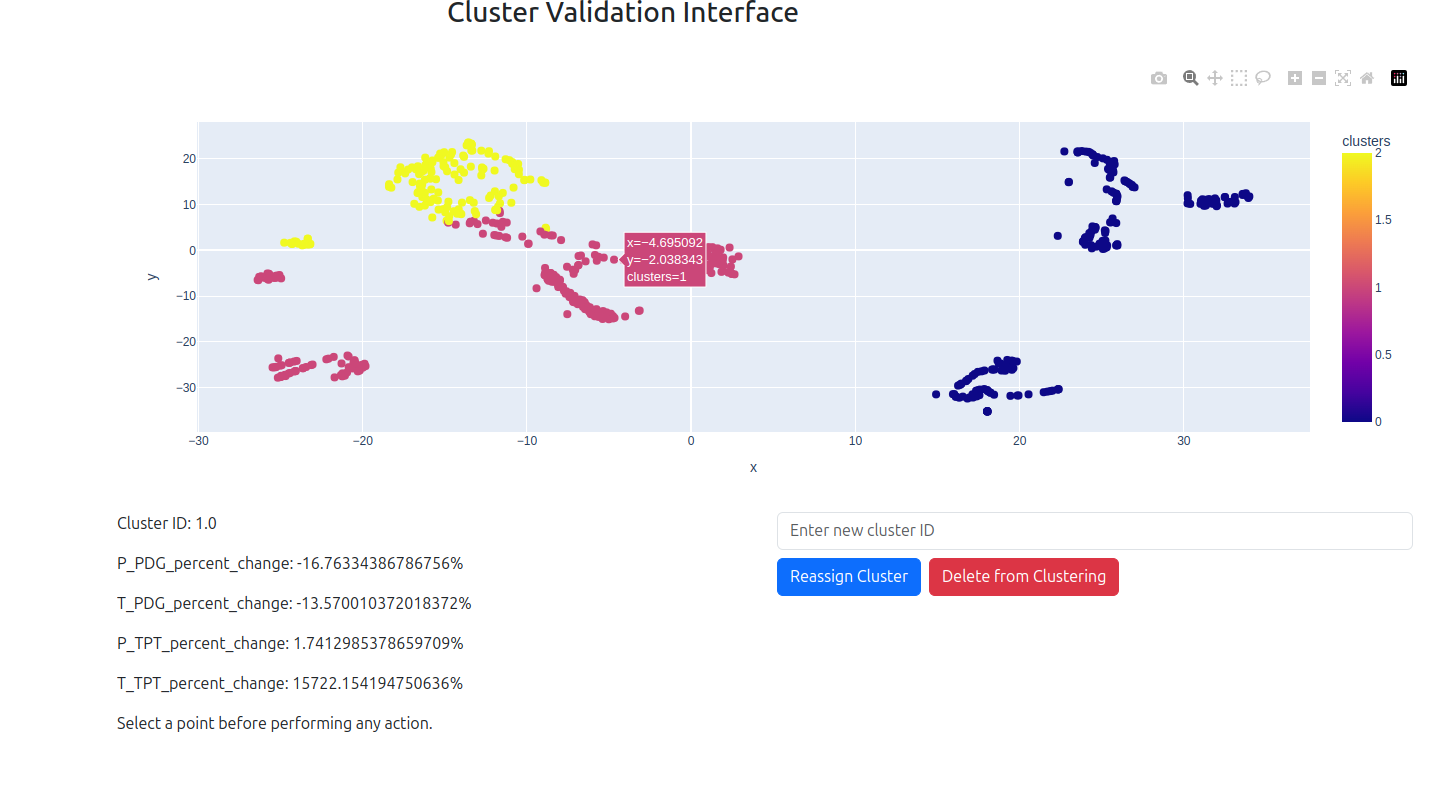
\includegraphics[width=\textwidth]{operator_mockup_interface.png}
\caption{Interface de validação de agrupamentos. O especialista inspeciona a projeção do
espaço latente, seleciona um ponto e recebe as variações percentuais por sensor daquele
segmento. Pode então reatribuir o ponto a outro agrupamento ou removê-lo da análise.}
\label{fig:oper-validacao}
\end{figure}

A \cref{fig:oper-validacao} materializa o laço humano do ciclo de mundo aberto. Três
decisões de projeto merecem comentário.

\textbf{A projeção é interativa, não estática.} O especialista precisa explorar, não
apenas contemplar. As ressalvas do \cref{cap:novidades} sobre projeções não lineares
valem aqui: a interface deve ser entendida como ferramenta de navegação, não como
representação fiel de distâncias.

\textbf{Cada ponto expõe suas estatísticas.} Selecionar um ponto revela as variações
percentuais por sensor --- as mesmas métricas do \cref{cap:agente}. O especialista julga
sobre números verificáveis, não sobre a posição visual.

\textbf{As ações são reversíveis e explícitas.} Reatribuir e remover, ambas registradas.
A remoção é particularmente importante: nem tudo que foi rejeitado merece virar classe.

\begin{destaque}[Note o valor de $15722\,\%$ na figura]
A variação percentual de T-TPT exibida é de mais de quinze mil por cento. Isso não é um
evento físico --- é o comportamento da \cref{eq:ag-pct} quando $\bar{b}$ é próximo de
zero, tipicamente porque o sensor estava congelado ou zerado no regime de base.

A interface expõe esse valor sem tratamento, e isso é uma virtude: o especialista
reconhece imediatamente um artefato de instrumentação. Uma interface que ``limpasse'' o
número o esconderia.

É também mais uma manifestação do artefato de telemetria que o
\cref{cap:resultados-agente} identificou.
\end{destaque}

\section{O laço humano}

\subsection{Três papéis distintos}

\begin{description}[leftmargin=0pt,style=nextline,itemsep=0.4em]

\item[Operador de turno.] Recebe alertas graduados, decide se investiga, registra o
desfecho. Precisa de latência baixa e de baixa taxa de falso alarme.

\item[Especialista de disciplina.] Valida agrupamentos, nomeia classes virtuais, corrige
perfis. Atua em escala de dias, não de minutos.

\item[Responsável pelo modelo.] Monitora deriva, decide retreinamentos, versiona
modelos e prompts.

\end{description}

Confundir esses papéis é um erro comum. A interface do operador não deve expor controles
de validação de agrupamento; a do especialista não precisa de latência de segundos.

\subsection{Governança de classes virtuais}

Um sistema que promove classes virtuais indefinidamente acumula categorias mal definidas.
A \cref{tab:oper-governanca} propõe uma política.

\begin{table}[htbp]
\centering
\caption{Política de governança de classes virtuais.}
\label{tab:oper-governanca}
\small
\begin{tabular}{p{3.2cm}p{8.8cm}}
\toprule
\textbf{Decisão} & \textbf{Critério} \\
\midrule
Promover a virtual &
Grupo aprovado nos três índices internos; ao menos trinta segmentos; convergência de
nomes acima de um limiar \\
\addlinespace
Encaminhar a revisão &
Toda classe virtual, dentro de um prazo definido, com o nome e a justificativa do
agente \\
\addlinespace
Fundir &
Dois grupos cujas descrições convergem para o mesmo nome e cujos centroides distam menos
que um limiar \\
\addlinespace
Descartar &
Grupo cuja dispersão de nomes indica confabulação; grupo dominado por artefato de
instrumentação \\
\addlinespace
Promover a real &
Confirmação do especialista, com definição por mecanismo e não por sintoma \\
\bottomrule
\end{tabular}
\end{table}

\begin{destaque}[A última linha é a mais importante]
``Definição por mecanismo e não por sintoma'' é a lição que as classes 4 e 5 ensinaram ao
longo de todo o livro. Uma política de governança que não a incorpore reproduzirá o
problema em cada nova classe.
\end{destaque}

\section{Deriva}

\subsection{Três formas}

\begin{description}[leftmargin=0pt,style=nextline,itemsep=0.4em]

\item[Deriva de dados.] A distribuição das entradas muda --- o poço envelhece, o BSW
sobe, a pressão de reservatório cai. O modelo continua correto sobre o passado e
progressivamente irrelevante sobre o presente.

\item[Deriva de conceito.] A relação entre entrada e rótulo muda. Um mesmo padrão de
sensores passa a significar outra coisa, por exemplo após uma intervenção que altera a
completação.

\item[Deriva induzida pelo próprio sistema.] O caso mais insidioso: o modelo se retreina
sobre dados que ele mesmo classificou como normais e, gradualmente, aprende a considerar
normal uma degradação progressiva.

\end{description}

\begin{destaque}[A salvaguarda do \cref{cap:dual}, revisitada]
A regra de excluir dados anômalos do conjunto de retreinamento existe precisamente para
impedir a terceira forma. Sem ela, uma incrustação que se desenvolve ao longo de meses
seria progressivamente absorvida como normalidade, e o alarme se extinguiria sozinho ---
sem que nenhuma métrica indicasse falha.

É o modo de falha mais perigoso de sistemas auto-adaptativos, porque é silencioso.
\end{destaque}

\subsection{O que monitorar}

\begin{itemize}[leftmargin=*,itemsep=0.3em]
  \item \textbf{Distribuição do escore de Mahalanobis} sobre dados classificados como
        normais. Um deslocamento sistemático indica deriva de dados.
  \item \textbf{Taxa de rejeição.} Um aumento sustentado pode indicar deriva ou o
        surgimento de um fenômeno novo --- e distinguir os dois é trabalho do
        especialista.
  \item \textbf{Taxa de confirmação do agente.} Queda na fração de decisões validadas
        sugere que os perfis de classe estão desatualizados.
  \item \textbf{Convergência de nomes.} Aumento de dispersão indica que o agente está
        confabulando com mais frequência.
  \item \textbf{Desfecho registrado pelo operador.} A única fonte de rótulo verdadeiro
        em operação, e a mais valiosa.
\end{itemize}

\begin{destaque}[Quatro dos cinco indicadores não exigem rótulo]
Isso é essencial. Um esquema de monitoramento que dependesse de rótulos seria inútil
exatamente onde é mais necessário --- em operação contínua, sem anotação.

O quinto indicador, o desfecho registrado, exige disciplina operacional e é o mais
difícil de obter. Vale investir nele: é o que permite avaliar o sistema de verdade.
\end{destaque}

\section{Custo}

\begin{table}[htbp]
\centering
\caption{Estrutura de custo por camada, em ordem de grandeza.}
\label{tab:oper-custo}
\small
\begin{tabular}{p{3.4cm}p{4.2cm}p{4.4cm}}
\toprule
\textbf{Camada} & \textbf{Custo de inferência} & \textbf{Observação} \\
\midrule
Diagrama de decisão & Desprezível & Regras \\
U-Net & Milissegundos por sensor & GPU opcional \\
Ensemble binário & \SI{405}{\milli\second}; \SI{21}{\mega\byte} & Por poço \\
Mahalanobis & Desprezível & Inversão de matriz $64 \times 64$ pré-computada \\
Agente de linguagem & Segundos; custo por chamada & \textbf{Somente sobre segmentos anômalos} \\
\bottomrule
\end{tabular}
\end{table}

\begin{destaque}[A decisão de custo que viabiliza a camada de linguagem]
Acionar o agente a cada janela, em duzentos e cinquenta poços, seria proibitivo em custo
e desnecessário: a esmagadora maioria das janelas é normal.

Acioná-lo apenas sobre segmentos que a camada 4 sinalizou reduz o volume em ordens de
grandeza --- de milhões de janelas por dia para dezenas de segmentos. É por isso que a
arquitetura do \cref{cap:sintese} coloca o agente na posição seis, e não na posição um.

Generalizando: em sistemas com componentes de custo muito assimétrico, a arquitetura
deve garantir que o componente caro só seja acionado quando o barato já filtrou.
\end{destaque}

\subsection{Custos que não aparecem na tabela}

\begin{itemize}[leftmargin=*,itemsep=0.3em]
  \item \textbf{Tempo do especialista} na validação de classes virtuais. É o custo
        dominante do ciclo de mundo aberto, e a razão pela qual as descrições geradas
        pelo agente têm valor econômico direto.
  \item \textbf{Versionamento de modelos e prompts.} Um prompt é código; deve ser
        versionado, revisado e testado.
  \item \textbf{Dependência de serviço externo.} Disponibilidade, latência de rede,
        mudança de modelo sem aviso.
  \item \textbf{Governança de dados.} Enviar dados operacionais a um serviço de terceiros
        exige avaliação de conformidade.
\end{itemize}

\section{Uma lista de verificação}

\begin{enumerate}[leftmargin=*,itemsep=0.3em]
  \item O sistema funciona no primeiro segundo, antes de qualquer treinamento?
  \item Ele informa explicitamente quando não sabe?
  \item Ele degrada graciosamente quando um sensor falha?
  \item Manobras deliberadas geram alarme?
  \item O desempenho foi reportado com desvio padrão entre poços?
  \item Cada afirmação do sistema pode ser rastreada a um número verificável?
  \item Indicadores discordantes são apresentados separadamente?
  \item Existe caminho para o operador registrar o desfecho?
  \item Existe política escrita de governança de classes novas?
  \item O monitoramento de deriva dispensa rótulos?
  \item O componente caro só é acionado após filtragem pelo barato?
  \item Prompts e modelos estão versionados?
\end{enumerate}

\resumocapitulo{%
A distância entre um protótipo e um sistema implantado é feita de requisitos não
funcionais que nenhuma métrica captura: disponibilidade desde o primeiro segundo,
operação sem rotulação contínua, robustez a falha de sensor e a manobra deliberada,
auditabilidade e extensibilidade. A interface deve apresentar separadamente a
delimitação, a decisão conhecido/novidade, a classe e as hipóteses do agente --- fundir
indicadores é aceitável quando concordam e inaceitável quando discordam, e como não se
sabe de antemão, não se funde. O laço humano envolve três papéis com necessidades
distintas: operador de turno, especialista de disciplina e responsável pelo modelo. A
governança de classes virtuais define quando promover, fundir, descartar e --- crucialmente
--- exige que a promoção a classe real seja feita por mecanismo, não por sintoma. Das
três formas de deriva, a mais perigosa é a induzida pelo próprio sistema, contra a qual a
exclusão de dados anômalos do retreinamento é a salvaguarda. Quatro dos cinco indicadores
de deriva propostos dispensam rótulos. Por fim, a camada de linguagem só é
economicamente viável porque é acionada apenas sobre segmentos já filtrados: em sistemas
com custos assimétricos, o componente caro deve vir depois do barato.}

\begin{exercicios}
\item Estime o volume diário de janelas processadas em duzentos e cinquenta poços com
      inferência a cada minuto, e o número esperado de segmentos anômalos com taxa de
      falso alarme de $5\,\%$. Quantas chamadas ao agente isso representa por dia?

\item Projete a interface do operador de turno com os quatro objetos produzidos pelo
      sistema. Justifique cada elemento visual em termos de carga cognitiva e de risco de
      fadiga de alarme.

\item Implemente os cinco indicadores de deriva propostos. Simule uma deriva de dados
      lenta sobre um poço do 3W e verifique quais indicadores a detectam e com quanta
      antecedência.

\item Construa um cenário concreto de deriva induzida pelo próprio sistema e demonstre,
      por simulação, que a salvaguarda de exclusão de dados anômalos a impede. O que
      acontece se a salvaguarda tiver falsos negativos?

\item A \cref{fig:oper-validacao} exibe uma variação percentual de mais de quinze mil por
      cento. Proponha três formas de apresentar esse valor ao especialista --- exibir sem
      tratamento, limitar a uma faixa, ou substituir por uma marca de artefato --- e
      discuta os riscos de cada uma.

\item Redija a política de governança de classes virtuais como documento operacional,
      com critérios numéricos concretos, prazos e responsáveis. Aplique-a
      retrospectivamente aos agrupamentos do \cref{cap:mundoaberto}.

\item Percorra a lista de verificação para um sistema de aprendizado de máquina com que
      você tenha trabalhado. Quantos itens ele satisfaz? Para cada item não satisfeito,
      estime o custo de corrigi-lo.
\end{exercicios}

\begin{leituras}
\item \citet{aranha2023system} e \citet{Aranha2024} --- descrições de sistemas de
      monitoramento em operação real.
\item \citet{LopesTese2025} --- o contexto operacional completo do sistema dual.
\item \citet{nodered} --- a ferramenta de orquestração usada na implantação.
\item \citet{gatta2022predictive} e \citet{soriano2021visual} --- aspectos operacionais e
      de visualização em monitoramento de poços.
\end{leituras}

\chapter{O que ainda não sabemos}
\label{cap:futuro}

\begin{objetivos}
Ao final deste capítulo, você será capaz de:
\begin{itemize}[leftmargin=*,itemsep=0.2em]
  \item enunciar com precisão as limitações que atravessam todo o trabalho apresentado;
  \item distinguir limitações de dados, de método e de avaliação;
  \item formular questões de pesquisa a partir de resultados negativos e de artefatos
        identificados;
  \item avaliar criticamente afirmações sobre sistemas de detecção de anomalias em
        contextos industriais;
  \item planejar uma agenda de trabalho que ataque os gargalos na ordem correta.
\end{itemize}
\end{objetivos}

\section{Uma advertência sobre o que foi medido}

Este livro apresentou muitos números. Antes de propor o que vem depois, é necessário
delimitar o que esses números sustentam.

\begin{destaque}[A ressalva que atravessa tudo]
Quatro classes receberam, do agente, nomes contendo ``perda de telemetria''
(\cref{cap:resultados-agente}). Isso revelou que, no 3W, o início de muitas anomalias
coincide com sensores de fundo reportando valores ausentes ou zerados.

A implicação é desconfortável: \textbf{parte do desempenho reportado nos experimentos
com o 3W pode decorrer da detecção de falha de instrumentação, e não da detecção da
anomalia}. Não há como quantificar essa fração com os experimentos realizados.

As análises por matriz de confusão apresentadas não evidenciaram esse padrão; as
descrições em linguagem natural o tornaram visível e motivam um teste controlado.
\end{destaque}

Essa ressalva não invalida automaticamente os resultados --- o \cref{cap:dual} reporta
estudos de caso de campo com dados reais e eventos verificados --- mas define a primeira
prioridade da agenda: \emph{medir o confundimento antes de perseguir mais acurácia}.

\section{Limitações de dados}

\begin{enumerate}[leftmargin=*,itemsep=0.4em]

\item \textbf{Possível confundimento de telemetria.} Descrito acima. Testável por um protocolo
que remova instâncias em que a anomalia coincide com valores ausentes, e repita toda a
avaliação. A diferença de desempenho pareada, com intervalo de confiança, estimará a
contribuição desse sinal; a remoção também pode alterar a composição e a dificuldade da
amostra.

\item \textbf{Um único conjunto de dados.} Quase tudo foi avaliado no 3W. A exceção ---
o sistema dual, avaliado em poços reais de um operador --- é justamente a que não permite
publicação dos dados.

\item \textbf{Amostras pequenas por classe.} A classe 9 tem $n = 11$ no estudo de
novidade e $n = 14$ no de classificação. Intervalos de confiança de Wilson com essas
amostras são largos o bastante para tornar várias comparações inconclusivas.

\item \textbf{Rótulos de qualidade heterogênea.} A análise do poço A3 no
\cref{cap:segmentacao} mostrou que a discordância entre modelo e anotação podia ser
atribuída à anotação. Não se sabe quantos outros casos assim existem.

\item \textbf{Classes definidas por sintoma.} As classes 4 e 5, discutidas em quatro
capítulos. Não é um problema de método.

\item \textbf{Possível contaminação.} O 3W é público desde 2019 e pode ter integrado
corpora de pré-treinamento. O \cref{cap:resultados-agente} apresentou três argumentos
contra essa explicação, nenhum deles conclusivo.

\end{enumerate}

\begin{destaque}[Cinco das seis limitações são do conjunto de dados, não do método]
Isso é característico da área. A comunidade de detecção de anomalias industriais dispõe
de poucos conjuntos públicos, e o 3W --- apesar de todas as ressalvas --- é um dos
melhores existentes.

Avançar exige mais dados públicos de qualidade, com anotação por especialista e taxonomia
por mecanismo. É trabalho menos glamouroso que propor arquiteturas, e provavelmente mais
impactante.
\end{destaque}

\section{Limitações de método}

\subsection{Segmentação}

A U-Net exige anotação por amostra, muito mais cara que anotação por janela. O
\cref{cap:segmentacao} obteve $0{,}863$ de acurácia com esse custo. Não se sabe qual
seria o desempenho de abordagens fracamente supervisionadas, que aprendem a segmentar a
partir de rótulos de janela.

A revocação SoftED de $0{,}678$ significa que cerca de um terço dos eventos não é
detectado dentro da tolerância temporal. A detecção antecipada de $0{,}222$ indica que o
modelo raramente antecipa o especialista --- e antecipar é o que teria valor operacional.

\subsection{Novidade}

A média $\bm{\mu}$ e a covariância $\bm{\Sigma}$ do Mahalanobis são estimadas uma vez, e
não acompanham deriva. Um esquema de atualização incremental é necessário, mas introduz o
risco de absorver degradação progressiva --- o modo de falha silencioso do
\cref{cap:operacao}.

O limiar no percentil 95 é uma escolha, não uma derivação. A justificativa dada no
\cref{cap:mahalanobis} --- que a hipótese de normalidade multivariada não se sustenta ---
explica por que não se usa $\chi^2$, mas não estabelece que 95 seja ótimo.

A classe 7 permanece em $52{,}3\,\%$. O diagnóstico é claro: a janela de duzentos passos
não comporta um fenômeno de semanas. A solução exige representação multiescala.

\subsection{Agente}

\begin{itemize}[leftmargin=*,itemsep=0.3em]
  \item \textbf{Sem ablação.} Não se sabe quais das treze métricas importam. Um estudo de
        ablação é o experimento de menor custo e maior retorno informativo pendente.
  \item \textbf{Sem comparação com atribuição.} SHAP e gradientes integrados produzem
        explicações de natureza diferente; não foram comparados.
  \item \textbf{Sem ajuste fino, sem exemplos, sem múltiplas passagens, sem ferramentas.}
        Como o \cref{cap:agente} registrou, os resultados devem ser lidos como piso.
  \item \textbf{Sem calibração.} A confiança declarada pelo agente não foi verificada
        contra frequências empíricas.
  \item \textbf{Sem informação de localização.} A confusão entre as classes 8 e 9 decorre
        disso, e é corrigível.
\end{itemize}

\subsection{Reprodutibilidade do modelo de linguagem}

O \cref{cap:llm} prometeu que este capítulo discutiria alternativas. A questão é séria:
o modelo é servido por interface de programação de terceiros, pode ser atualizado ou
descontinuado sem aviso, e a temperatura de $0{,}2$ reduz mas não elimina a
estocasticidade. Os resultados não são estritamente reproduzíveis.

\begin{table}[htbp]
\centering
\caption{Alternativas para reprodutibilidade da camada de linguagem.}
\label{tab:fut-repro}
\small
\begin{tabular}{p{3.0cm}p{4.4cm}p{4.6cm}}
\toprule
\textbf{Alternativa} & \textbf{Ganho} & \textbf{Custo} \\
\midrule
Modelo aberto local, versão fixa &
Reprodutibilidade estrita; dados não saem do perímetro &
Infraestrutura de GPU; desempenho tipicamente inferior \\
\addlinespace
Ajuste fino sobre modelo aberto menor &
Adaptação ao domínio; modelo próprio e versionável &
Exige dados rotulados --- o que o sistema procura evitar \\
\addlinespace
Registro completo de entradas e saídas &
Auditoria posterior; permite reanálise &
Não permite repetir o experimento \\
\addlinespace
Amostragem múltipla com agregação &
Reduz variância; mede consistência &
Multiplica o custo por chamada \\
\bottomrule
\end{tabular}
\end{table}

\begin{destaque}[Não há escolha dominante]
Cada linha da \cref{tab:fut-repro} troca uma propriedade desejável por outra. A
recomendação prática é combinar a terceira linha --- registro completo, que é barata e
compatível com qualquer das outras --- com a alternativa que o contexto de governança
exigir.

Em ambiente industrial com restrição de dados, a primeira linha tende a ser mandatória,
e o custo de desempenho deve ser aceito.
\end{destaque}

\section{Limitações de avaliação}

\begin{enumerate}[leftmargin=*,itemsep=0.4em]

\item \textbf{Nenhuma avaliação com operadores.} Todas as afirmações sobre carga
cognitiva, fadiga de alarme e utilidade das justificativas são argumentadas, não medidas.
A política de triagem do \cref{cap:resultados-agente} --- que reduziria à metade o volume
de revisão --- é uma projeção.

\item \textbf{Nenhuma avaliação fim-a-fim.} Os componentes foram medidos isoladamente. A
arquitetura de referência do \cref{cap:sintese} nunca foi executada como um todo.

\item \textbf{Ausência de linha de base humana.} Não se sabe qual é a acurácia de um
especialista sobre os mesmos segmentos, o que impede afirmar que o sistema é útil e não
apenas mensurável.

\item \textbf{Comparações com a literatura são aproximadas.} Como o \cref{cap:binarios}
registrou, protocolos, partições e definições de classe diferem entre trabalhos.

\end{enumerate}

\begin{destaque}[A limitação mais séria é a terceira]
Sem linha de base humana, ``$89{,}7\,\%$ de detecção de novidade'' é um número sem
referencial. Pode ser excelente ou trivial.

Estabelecer essa linha de base é caro --- exige tempo de especialista --- e é a lacuna
que mais compromete a interpretação de todo o trabalho.
\end{destaque}

\section{Uma agenda}

\subsection{Ordenada por razão informação/custo}

\begin{table}[htbp]
\centering
\caption{Agenda de trabalho, ordenada por razão entre informação obtida e custo.}
\label{tab:fut-agenda}
\small
\begin{tabular}{p{5.2cm}p{2.0cm}p{4.8cm}}
\toprule
\textbf{Experimento} & \textbf{Custo} & \textbf{Informação obtida} \\
\midrule
Remoção do confundimento de telemetria & Baixo &
Quantifica quanto do desempenho é artefato \\
\addlinespace
Ablação das treze métricas & Baixo &
Quais métricas importam; guia para adicionar novas \\
\addlinespace
Métricas de localização por sensor & Baixo &
Testa a hipótese sobre a confusão entre classes 8 e 9 \\
\addlinespace
Calibração da confiança declarada & Baixo &
Viabiliza uso da confiança na política de triagem \\
\addlinespace
Múltiplas passagens com agregação & Médio &
Mede consistência; provável ganho em top-1 \\
\addlinespace
Representação multiescala & Médio &
Ataca a classe 7 diretamente \\
\addlinespace
Avaliação fim-a-fim da arquitetura & Médio &
Único número que descreve o sistema real \\
\addlinespace
Segmentação fracamente supervisionada & Alto &
Elimina o custo de anotação por amostra \\
\addlinespace
Linha de base humana & Alto &
Referencial para todos os números do livro \\
\addlinespace
Redefinição das classes sintomáticas & Alto &
Corrige a taxonomia; beneficia toda a comunidade \\
\bottomrule
\end{tabular}
\end{table}

\subsection{Quatro questões de pesquisa}

\begin{description}[leftmargin=0pt,style=nextline,itemsep=0.5em]

\item[A assimetria é universal?] Métodos geométricos e modelos de linguagem, sistemas de
natureza completamente distinta, exibem a mesma assimetria entre afirmar identidade e
reconhecer incompatibilidade. Ela se manifesta em outros domínios? Existe uma formulação
teórica que a preveja?

\item[A convergência de nomes é uma métrica de confiança válida?] O
\cref{cap:resultados-agente} propôs medir a concentração das descrições geradas como
indicador não supervisionado de confiabilidade. A proposta é plausível e não foi
validada. Se funcionar, resolve o problema de estimar confiança sem rótulos.

\item[Quanto da vantagem do latente supervisionado é transferível?] O
\cref{cap:mahalanobis} mostrou que representar com um classificador em vez de um
autoencoder eleva a detecção de novidade em quarenta e seis pontos. Isso depende de haver
classes conhecidas suficientes. Qual é o mínimo? A vantagem persiste com três classes?
Com duas?

\item[Sistemas que descrevem auditam melhor os dados?] O artefato de telemetria do 3W só
se tornou visível pela descrição em linguagem natural. Isso sugere um uso não previsto de
modelos de linguagem: auditoria automática de conjuntos de dados. A hipótese pode ser
testada injetando artefatos conhecidos e verificando se são descritos.

\end{description}

\section{Encerramento}

\begin{destaque}[O que este livro sustenta]
Um sistema de monitoramento pode --- e deve --- dizer ``não sei''.

Dizer isso corretamente é mais fácil do que dizer o que algo é: $95{,}4\,\%$ contra
$87\,\%$ nos métodos numéricos, $89{,}7\,\%$ contra $35{,}1\,\%$ na camada de linguagem.

O espaço em que a pergunta é feita importa mais que o método: a mesma distância detecta
$67{,}5\,\%$ ou $98{,}2\,\%$ da mesma anomalia.

E um sistema que descreve o que vê, em linguagem que o especialista lê, transforma um
grupo anônimo em uma hipótese verificável --- além de revelar problemas nos dados que
nenhuma métrica agregada exporia.

Nada disso substitui o especialista. Tudo isso muda o que ele recebe no início do turno.
\end{destaque}

\resumocapitulo{%
Os resultados deste livro devem ser lidos sob uma ressalva que atravessa todos os
capítulos: no 3W, o início de muitas anomalias coincide com falha de telemetria, e parte
do desempenho reportado pode decorrer da detecção desse artefato --- fração que os
experimentos realizados não permitem quantificar. Cinco das seis limitações de dados são
do conjunto, não do método, o que aponta a escassez de dados públicos de qualidade como
gargalo da área. Entre as limitações de método, destacam-se a revocação SoftED de
$0{,}678$ e a detecção antecipada de $0{,}222$ na segmentação; a estimação estática de
$\bm{\mu}$ e $\bm{\Sigma}$ no Mahalanobis; a classe 7 presa em $52{,}3\,\%$ por
insuficiência de escala temporal; e, no agente, a ausência de ablação, de calibração e de
métricas de localização. A reprodutibilidade da camada de linguagem não tem solução
dominante: cada alternativa troca uma propriedade desejável por outra, e o registro
completo de entradas e saídas é a única compatível com todas as demais. A limitação de
avaliação mais séria é a ausência de linha de base humana, sem a qual os números do livro
carecem de referencial. A agenda proposta ordena dez experimentos por razão entre
informação e custo, com a avaliação do possível confundimento de telemetria em primeiro
lugar, e formula quatro
questões de pesquisa --- entre elas, se a assimetria entre reconhecer incompatibilidade e
afirmar identidade é uma propriedade universal.}

\begin{projetospesquisa}
\item Projete e execute o estudo de ablação das treze métricas do \cref{cap:agente}.
      Ordene-as por contribuição marginal. O resultado é consistente com a intuição
      física?

\item Implemente o protocolo de remoção do confundimento de telemetria e reavalie os
      resultados dos \cref{cap:binarios,cap:mahalanobis,cap:resultados-agente}. Quanta
      acurácia se perde em cada um? A ordenação entre métodos se mantém?

\item Verifique a calibração da confiança declarada pelo agente construindo um diagrama
      de confiabilidade. Se ela estiver mal calibrada, proponha e avalie uma correção.

\item Ataque a classe 7 com uma representação multiescala --- por exemplo, concatenando
      latentes de janelas de duzentos, dois mil e vinte mil passos. Quanto se ganha? O
      que se perde nas demais classes?

\item Estime experimentalmente o número mínimo de classes conhecidas necessário para que
      o latente supervisionado supere o latente do autoencoder na detecção de novidade.

\item Teste a hipótese de auditoria automática: injete um artefato conhecido em um
      conjunto de dados limpo e verifique se o agente o descreve. Varie a intensidade do
      artefato e determine o limiar de detecção.

\item Projete o protocolo de uma avaliação com operadores que meça, e não apenas
      argumente, a redução de carga de revisão prometida pela política de triagem do
      \cref{cap:resultados-agente}. Que ameaças à validade ele precisa controlar?
\end{projetospesquisa}

\begin{leituras}
\item \citet{Pimentel2014review} --- levantamento que contextualiza as limitações
      discutidas neste capítulo.
\item \citet{Salles2024softed} --- a métrica cujos valores de revocação e detecção
      antecipada apontam as lacunas da segmentação.
\item \citet{VazVargas2026_3w2} --- a evolução do 3W, e o caminho pelo qual várias das
      limitações de dados podem ser atacadas.
\item \citet{Sharma2025xaiagents}, \citet{Belay2026agenticAD} e \citet{Zhang2026llmrules}
      --- direções contemporâneas para a camada de linguagem.
\end{leituras}


% ---------------------------------------------------------------------------
\appendix
% ---------------------------------------------------------------------------
\chapter{Glossário}
\label{cap:glossario}

Este apêndice reúne os termos técnicos empregados no livro, com a definição usada aqui e
o original em inglês. A lista de siglas encontra-se nas páginas pré-textuais.

\section{Operação de poços e escoamento}

\begin{description}[leftmargin=0pt,style=nextline,itemsep=0.35em]

\item[Anomalia] Comportamento do poço que se desvia do regime operacional esperado. Não
é sinônimo de falha: uma anomalia pode ser benigna, e uma falha pode ocorrer sem
anomalia detectável nos sensores disponíveis.

\item[Árvore de natal molhada (\ing{wet christmas tree})] Conjunto de válvulas instalado
na cabeça do poço submarino, que controla o fluxo entre o poço e as linhas de produção.

\item[Completação inteligente (\ing{intelligent completion})] Arranjo de poço com
válvulas de controle de intervalo operáveis remotamente, que permite regular a
contribuição de cada zona produtora sem intervenção física.

\item[Curva de formação de hidrato] Fronteira no plano pressão--temperatura que separa a
região onde hidratos de gás são termodinamicamente estáveis da região onde não são.

\item[Elevação por gás (\ing{gas lift})] Técnica de elevação artificial em que gás é
injetado na coluna de produção para reduzir a densidade da mistura e restabelecer o
fluxo.

\item[Golfada (\ing{slugging})] Regime de escoamento intermitente em que bolsões de gás
e de líquido alternam-se, produzindo oscilações de pressão e vazão.

\item[Hidrato de gás] Sólido cristalino formado por moléculas de gás aprisionadas em uma
estrutura de água, estável a alta pressão e baixa temperatura. Pode obstruir linhas de
produção.

\item[Incrustação (\ing{scaling})] Deposição progressiva de sais ou parafinas nas
paredes da tubulação ou na válvula reguladora, que restringe o fluxo ao longo de semanas
ou meses.

\item[Intervenção] Operação física sobre o poço, geralmente com embarcação dedicada, de
custo elevado. Reduzir intervenções não programadas é um dos objetivos do monitoramento.

\item[Linha de serviço] Linha secundária, distinta da linha de produção, usada para
injeção de químicos, gás de elevação ou operações auxiliares.

\item[Perda de produtividade] Redução sustentada da vazão produzida sob condições
operacionais equivalentes.

\item[Poço injetor] Poço destinado a injetar fluido no reservatório, para manutenção de
pressão ou varrido, em oposição ao poço produtor.

\item[Pré-sal] Província petrolífera brasileira situada abaixo de uma camada de sal, em
lâminas d'água tipicamente superiores a dois mil metros.

\item[Regime permanente (\ing{steady state})] Condição em que as variáveis do processo
permanecem aproximadamente constantes, em oposição ao transiente.

\item[Tempo não produtivo] Período em que o poço não produz por razão não programada.

\item[Transiente] Período de variação rápida das variáveis do processo, tipicamente após
uma manobra deliberada, durante o qual os modelos de regime permanente não se aplicam.

\item[Válvula de controle de intervalo] Válvula de fundo que regula a contribuição de
uma zona produtora específica.

\item[Válvula de segurança de subsuperfície] Válvula de fundo que fecha automaticamente
em condição de emergência, isolando o poço.

\item[Válvula reguladora de produção (\ing{production choke})] Válvula que controla a
vazão do poço para a linha de produção.

\end{description}

\section{Aprendizado de máquina}

\begin{description}[leftmargin=0pt,style=nextline,itemsep=0.35em]

\item[Acurácia balanceada] Média das revocações por classe. Usada quando as classes são
desbalanceadas, situação em que a acurácia simples é enganosa.

\item[Agrupamento (\ing{clustering})] Tarefa não supervisionada de particionar um
conjunto de dados em grupos de elementos semelhantes.

\item[Aprendizado de mundo aberto (\ing{open-world learning})] Paradigma em que o modelo
deve reconhecer que uma amostra não pertence a nenhuma classe conhecida, organizar as
amostras rejeitadas e incorporá-las como novas classes.

\item[Aprendizado de mundo fechado (\ing{closed-world learning})] Paradigma que pressupõe
que todas as classes que ocorrerão em operação estavam presentes no treinamento.

\item[Atenção (\ing{attention})] Mecanismo que pondera dinamicamente a contribuição de
cada posição de uma sequência, permitindo caminho de comprimento constante entre
posições distantes.

\item[Autoencoder] Rede treinada para reconstruir a própria entrada através de um
gargalo, aprendendo uma representação comprimida sem supervisão.

\item[Classe virtual] Agrupamento de amostras rejeitadas que satisfaz critérios de
coesão e é tratado provisoriamente como classe, até validação por especialista.

\item[Classe sintomática] Classe definida pelo sintoma observável e não pelo mecanismo
físico subjacente. Instâncias de uma mesma classe sintomática podem ter causas distintas,
o que compromete a coerência interna do rótulo.

\item[Deriva (\ing{drift})] Mudança, ao longo do tempo, da distribuição dos dados
(deriva de dados) ou da relação entre entrada e rótulo (deriva de conceito).

\item[Detecção de novidade (\ing{novelty detection})] Tarefa de identificar amostras que
não pertencem a nenhuma classe conhecida.

\item[Distância de Mahalanobis] Distância entre um ponto e uma distribuição, normalizada
pela covariância. É invariante a escala e sensível à correlação entre variáveis.

\item[Ensemble] Conjunto de modelos cujas saídas são combinadas. Neste livro, designa
sobretudo o conjunto de classificadores binários um-contra-todos.

\item[Época (\ing{epoch})] Uma passagem completa pelo conjunto de treinamento.

\item[Escore-$z$ (\ing{z-score})] Padronização que subtrai a média e divide pelo desvio
padrão.

\item[Espaço latente] Espaço de representação intermediária aprendido por um modelo. Sua
geometria determina o que métodos baseados em distância conseguem detectar.

\item[Índice de Calinski-Harabasz] Razão entre dispersão entre grupos e dispersão dentro
dos grupos. Valores maiores indicam melhor separação.

\item[Índice de Davies-Bouldin] Média da similaridade de cada grupo com seu vizinho mais
próximo. Valores menores indicam melhor separação.

\item[Interseção sobre união] Razão entre a interseção e a união de duas regiões. Usada
para avaliar a qualidade de segmentações.

\item[Janela deslizante (\ing{sliding window})] Recorte de comprimento fixo que avança
sobre a série temporal com passo definido.

\item[Mistura de especialistas] Arquitetura em que apenas um subconjunto dos parâmetros
é ativado por entrada, permitindo modelos de grande capacidade com custo de inferência
reduzido.

\item[Parada antecipada (\ing{early stopping})] Interrupção do treinamento quando a
métrica de validação deixa de melhorar por um número definido de épocas.

\item[Perceptron de múltiplas camadas] Rede neural composta por camadas densas
sucessivas com não linearidades.

\item[Rede recorrente] Rede que processa sequências mantendo um estado interno atualizado
a cada passo.

\item[Regularização por abandono (\ing{dropout})] Técnica que desativa aleatoriamente
unidades durante o treinamento, reduzindo sobreajuste.

\item[Reconhecimento em conjunto aberto (\ing{open-set recognition})] Formulação em que o
modelo pode recusar-se a atribuir uma classe, mas não organiza nem incorpora as amostras
recusadas.

\item[Risco de espaço aberto] Formalização do risco de classificar como conhecida uma
região do espaço de características arbitrariamente distante dos dados de treinamento.

\item[Segmentação de séries temporais] Tarefa de atribuir um rótulo a cada instante da
série, em oposição a atribuir um rótulo a uma janela inteira.

\item[Silhueta] Medida, por amostra, de quão bem ela se ajusta ao próprio grupo em
comparação ao grupo mais próximo. Varia em $[-1,1]$.

\item[Sobreajuste (\ing{overfitting})] Ajuste excessivo aos dados de treinamento, com
perda de desempenho em dados novos.

\item[Um-contra-todos (\ing{one-vs-all})] Estratégia que decompõe um problema
multiclasse em vários problemas binários independentes.

\item[Validação cruzada estratificada] Partição em dobras que preserva a proporção das
classes em cada dobra.

\end{description}

\section{Modelos de linguagem}

\begin{description}[leftmargin=0pt,style=nextline,itemsep=0.35em]

\item[Alucinação (\ing{hallucination})] Produção de afirmação fluente e plausível que
não é sustentada pela entrada nem por fato verificável.

\item[Cadeia de raciocínio (\ing{chain-of-thought})] Texto intermediário produzido antes
da resposta final. Não deve ser confundido com explicação do processo computacional
efetivo.

\item[Calibração] Grau de correspondência entre a confiança declarada por um modelo e a
frequência empírica de acerto.

\item[Contaminação de dados] Presença, no corpus de pré-treinamento, de dados usados na
avaliação, o que invalida a interpretação dos resultados como generalização.

\item[Instrução de sistema (\ing{system prompt})] Instrução que define papel, restrições
e formato de saída, aplicada antes da entrada específica.

\item[Prompt] Entrada textual fornecida ao modelo de linguagem, incluindo instrução,
contexto e dados.

\item[Saída estruturada] Resposta em formato especificado, tipicamente JSON, que pode ser
validada programaticamente.

\item[Temperatura] Parâmetro que controla a aleatoriedade da amostragem. Valores baixos
tornam a saída mais determinística.

\item[Transformador (\ing{transformer})] Arquitetura baseada em atenção, sem recorrência,
que permite paralelização do processamento da sequência.

\end{description}

\section{Métricas e avaliação}

\begin{description}[leftmargin=0pt,style=nextline,itemsep=0.35em]

\item[Detecção antecipada] Fração de eventos detectados antes do instante anotado pelo
especialista. Métrica da família SoftED.

\item[Erro percentual absoluto médio simétrico] Métrica de erro de reconstrução limitada
e simétrica em relação a sobre e subestimação.

\item[Especificidade] Fração de negativos corretamente identificados.

\item[Intervalo de Wilson] Intervalo de confiança para proporção binomial, adequado a
amostras pequenas e a proporções próximas de zero ou um.

\item[Medida $F_1$] Média harmônica entre precisão e revocação.

\item[Precisão] Fração de predições positivas que estão corretas.

\item[Revocação] Fração de positivos reais que foram detectados. Também chamada de
sensibilidade.

\item[SoftED] Família de métricas de detecção de eventos com tolerância temporal, que
credita parcialmente detecções próximas ao instante anotado.

\item[Top-$k$] Métrica que considera acerto se a resposta correta está entre as $k$
primeiras posições de uma lista ordenada.

\end{description}

\chapter{Correspondência de notação}
\label{cap:notacao}

A notação do livro foi harmonizada. Este apêndice registra a correspondência com os
símbolos dos trabalhos originais, para que o leitor possa transitar entre as fontes sem
ambiguidade. A tabela de símbolos propriamente dita encontra-se nas páginas pré-textuais.

\section{Séries temporais e janelas}

\begin{table}[htbp]
\centering
\caption{Correspondência de notação para dados e janelas.}
\label{tab:notb-dados}
\small
\begin{tabular}{p{2.3cm}p{4.6cm}p{5.4cm}}
\toprule
\textbf{Neste livro} & \textbf{Significado} & \textbf{Nos trabalhos originais} \\
\midrule
$T$ &
Passos de tempo da janela &
\emph{window size}, \emph{sequence length}, $n_{\text{steps}}$; valores 200, 500 e a
varredura de 150 a 7500 do \cref{cap:closedworld} \\
\addlinespace
$S$ &
Número de sensores &
\emph{n\_features}, \emph{channels}; valores 4 e 5 conforme o capítulo \\
\addlinespace
$\mat{X} \in \R^{T \times S}$ &
Janela multivariada &
$X$, \emph{input tensor}, com forma $(T, S)$ na notação de \ing{frameworks} \\
\addlinespace
$\vect{b}$, $\vect{e}$ &
Janelas de linha de base e de evento &
\emph{baseline window} e \emph{event window} no \cref{cap:agente} \\
\addlinespace
$y$ &
Rótulo de classe &
\emph{class}, \emph{label}; no 3W, o código de 0 a 9 \\
\bottomrule
\end{tabular}
\end{table}

\begin{destaque}[Uma diferença de convenção que confunde]
Bibliotecas de aprendizado profundo descrevem a entrada como \emph{(batch, timesteps,
features)}. Este livro omite a dimensão de lote e escreve $\mat{X} \in \R^{T \times S}$.

Assim, a camada descrita nos trabalhos originais como \emph{Input(500, 5)} corresponde
aqui a $T = 500$ e $S = 5$.
\end{destaque}

\section{Modelos e representações}

\begin{table}[htbp]
\centering
\caption{Correspondência de notação para modelos.}
\label{tab:notb-modelos}
\small
\begin{tabular}{p{2.3cm}p{4.6cm}p{5.4cm}}
\toprule
\textbf{Neste livro} & \textbf{Significado} & \textbf{Nos trabalhos originais} \\
\midrule
$g_{\phi}$, $h_{\psi}$ &
Codificador e decodificador &
\emph{encoder} e \emph{decoder}; frequentemente sem símbolo, apenas nomeados \\
\addlinespace
$\vect{z}$ &
Representação latente &
\emph{latent vector}, \emph{embedding}, \emph{bottleneck}, \emph{latent
representation} \\
\addlinespace
$d$ &
Dimensão do latente &
\emph{latent dim}; valores 4, 16, 64 e 128 conforme o capítulo \\
\addlinespace
$c_k$, $s_k$ &
Classificador binário da classe $k$ e seu escore &
\emph{binary classifier k}, \emph{sigmoid output}, \emph{score} \\
\addlinespace
$\tau$ &
Limiar de decisão &
\emph{threshold}; valores 0,3, 0,5 e 0,65 conforme o contexto \\
\bottomrule
\end{tabular}
\end{table}

\begin{destaque}[Três latentes distintos, um mesmo símbolo]
O símbolo $\vect{z}$ designa, em capítulos diferentes, objetos com propriedades muito
distintas:

no \cref{cap:mundoaberto}, o latente de dimensão 16 de um autoencoder;

no \cref{cap:mahalanobis}, o latente de dimensão 128 de um autoencoder maior \emph{e} a
penúltima camada de dimensão 64 de um classificador multiclasse.

A tese central do \cref{cap:mahalanobis} é justamente que esses espaços não são
intercambiáveis, apesar de receberem o mesmo símbolo. Quando a distinção importa, o texto
a explicita.
\end{destaque}

\section{Estatística e limiares}

\begin{table}[htbp]
\centering
\caption{Correspondência de notação para estatística e limiares.}
\label{tab:notb-estat}
\small
\begin{tabular}{p{2.3cm}p{4.6cm}p{5.4cm}}
\toprule
\textbf{Neste livro} & \textbf{Significado} & \textbf{Nos trabalhos originais} \\
\midrule
$\mu + k\sigma$ &
Limiar de reconstrução &
\emph{mean + 3 std}; no \cref{cap:dual}, $k = 3$ \\
\addlinespace
$d_M$ &
Distância de Mahalanobis &
\emph{Mahalanobis distance}, $D^2$ quando elevada ao quadrado \\
\addlinespace
$\lambda$ &
Regularização da covariância &
\emph{shrinkage}, \emph{regularization term} somado à diagonal \\
\addlinespace
$K$ &
Número de agrupamentos &
$k$ minúsculo em \emph{k-means}; aqui maiúsculo, para evitar colisão \\
\addlinespace
$R = \mu/\sigma$ &
Razão do limiar adaptativo &
\emph{ratio} no \cref{cap:mundoaberto} \\
\addlinespace
$\delta = \bar{e} - \bar{b}$ &
Variação absoluta &
\emph{delta}, \emph{absolute change} no \cref{cap:agente} \\
\bottomrule
\end{tabular}
\end{table}

\section{Métricas}

\begin{table}[htbp]
\centering
\caption{Correspondência de notação para métricas de avaliação.}
\label{tab:notb-metricas}
\small
\begin{tabular}{p{2.3cm}p{4.6cm}p{5.4cm}}
\toprule
\textbf{Neste livro} & \textbf{Significado} & \textbf{Nos trabalhos originais} \\
\midrule
ACC & Acurácia & \emph{accuracy}, \emph{acc} \\
$\text{ACC}_b$ & Acurácia balanceada & \emph{balanced accuracy} \\
REC & Revocação & \emph{recall}, \emph{sensitivity}, \emph{true positive rate} \\
PR & Precisão & \emph{precision}, \emph{positive predictive value} \\
SP & Especificidade & \emph{specificity}, \emph{true negative rate} \\
$F_1$ & Medida F1 & \emph{F1-score}, \emph{F-measure} \\
IoU & Interseção sobre união & \emph{IoU}, \emph{Jaccard index} \\
\bottomrule
\end{tabular}
\end{table}

\begin{destaque}[Duas armadilhas de tradução]
\textbf{``Precisão''} traduz \emph{precision} neste livro, e nunca \emph{accuracy}. Em
português técnico corrente, ``precisão'' é usada às vezes para acurácia, o que gera
confusão. Aqui, acurácia é ACC e precisão é PR.

\textbf{``Sensibilidade''} e \textbf{``revocação''} são o mesmo objeto. O livro usa
revocação uniformemente, mas a literatura médica e de sinais prefere sensibilidade.
\end{destaque}

\section{Nomenclatura de classes}

\begin{table}[htbp]
\centering
\caption{Correspondência entre a numeração de classes do 3W e a designação usada no
livro.}
\label{tab:notb-classes}
\small
\begin{tabular}{clp{6.8cm}}
\toprule
\textbf{Código} & \textbf{Designação no livro} & \textbf{Denominação no 3W} \\
\midrule
0 & Normal & \emph{Normal} \\
1 & Aumento de BSW & \emph{Abrupt Increase of BSW} \\
2 & Fechamento de DHSV & \emph{Spurious Closure of DHSV} \\
3 & Golfadas severas & \emph{Severe Slugging} \\
4 & Instabilidade de fluxo & \emph{Flow Instability} \\
5 & Perda de produtividade & \emph{Rapid Productivity Loss} \\
6 & Restrição rápida no PCK & \emph{Quick Restriction in PCK} \\
7 & Incrustação no PCK & \emph{Scaling in PCK} \\
8 & Hidrato na produção & \emph{Hydrate in Production Line} \\
9 & Hidrato no serviço & \emph{Hydrate in Service Line} \\
\bottomrule
\end{tabular}
\end{table}

\begin{destaque}[Deslocamento de índice]
Alguns dos trabalhos originais indexam as nove classes anômalas de 1 a 9; outros indexam
de 0 a 8, tratando a classe normal separadamente. Este livro segue estritamente a
numeração do 3W, de 0 a 9, com a classe 0 correspondendo ao regime normal.

Ao comparar tabelas com as fontes originais, verifique a convenção antes de alinhar
linhas.
\end{destaque}

\chapter{Formulário}
\label{cap:formulario}

Este apêndice reúne, em um só lugar, as expressões usadas ao longo do livro. Cada uma
remete ao capítulo em que foi introduzida e discutida.

\section{Métricas de classificação}

Com VP, VN, FP e FN denotando verdadeiros positivos, verdadeiros negativos, falsos
positivos e falsos negativos (\cref{cap:aprendizado}):

\begin{align}
\text{ACC} &= \frac{\text{VP} + \text{VN}}{\text{VP} + \text{VN} + \text{FP} + \text{FN}}
\label{eq:for-acc} \\[0.4em]
\text{REC} &= \frac{\text{VP}}{\text{VP} + \text{FN}}
\label{eq:for-rec} \\[0.4em]
\text{SP} &= \frac{\text{VN}}{\text{VN} + \text{FP}}
\label{eq:for-sp} \\[0.4em]
\text{PR} &= \frac{\text{VP}}{\text{VP} + \text{FP}}
\label{eq:for-pr} \\[0.4em]
F_1 &= 2 \cdot \frac{\text{PR} \cdot \text{REC}}{\text{PR} + \text{REC}}
\label{eq:for-f1} \\[0.4em]
\text{ACC}_b &= \frac{1}{|\mathcal{K}|} \sum_{k \in \mathcal{K}} \text{REC}_k
\label{eq:for-accb}
\end{align}

Para segmentação, com $A$ e $B$ os conjuntos de instantes preditos e anotados:

\begin{equation}
\text{IoU} = \frac{|A \cap B|}{|A \cup B|}
\label{eq:for-iou}
\end{equation}

Para listas ordenadas de $N$ segmentos, com $\rho_i$ a posição da classe correta:

\begin{equation}
\text{top-}k = \frac{1}{N} \sum_{i=1}^{N} \mathbb{1}[\rho_i \le k]
\label{eq:for-topk}
\end{equation}

\section{Erro de reconstrução e limiar}

Erro percentual absoluto médio simétrico, usado como perda e como escore de anomalia
(\cref{cap:dual}):

\begin{equation}
\text{SMAPE} = \frac{100}{n} \sum_{i=1}^{n}
\frac{|\hat{x}_i - x_i|}{(|x_i| + |\hat{x}_i|)/2}
\label{eq:for-smape}
\end{equation}

Limiar sobre o erro de reconstrução, com $\mu$ e $\sigma$ estimados no conjunto de
treinamento e $k = 3$:

\begin{equation}
\tau = \mu + k\,\sigma
\label{eq:for-limiar}
\end{equation}

\section{Detecção de novidade}

Distância de Mahalanobis de um ponto $\vect{x}$ à distribuição de média $\bm{\mu}$ e
covariância $\bm{\Sigma}$ (\cref{cap:mahalanobis}):

\begin{equation}
d_M(\vect{x}) = \sqrt{(\vect{x} - \bm{\mu})^{\top}\,
\bm{\Sigma}^{-1}\,(\vect{x} - \bm{\mu})}
\label{eq:for-mahalanobis}
\end{equation}

Regularização da covariância, necessária quando a dimensão é comparável ao número de
amostras:

\begin{equation}
\bm{\Sigma}_{\text{reg}} = \bm{\Sigma} + \lambda \mat{I}
\label{eq:for-sigmareg}
\end{equation}

Decisão de novidade, com $\tau_{95}$ o percentil 95 das distâncias no conjunto de
referência:

\begin{equation}
\text{novidade}(\vect{x}) =
\begin{cases}
1, & d_M(\vect{x}) > \tau_{95} \\
0, & \text{caso contrário}
\end{cases}
\label{eq:for-decisao}
\end{equation}

Rejeição por ensemble binário (\cref{cap:binarios}), com $s_k$ o escore do classificador
da classe $k$:

\begin{equation}
\text{rejeitar} \iff \max_{k \in \mathcal{K}} s_k < \tau
\label{eq:for-rejeicao}
\end{equation}

Voto ponderado entre classificador latente e OCSVM (\cref{cap:mundoaberto}):

\begin{equation}
v = w_{\text{bin}}\, s_{\text{bin}} + w_{\text{ocsvm}}\, s_{\text{ocsvm}},
\qquad w_{\text{bin}} + w_{\text{ocsvm}} = 1
\label{eq:for-voto}
\end{equation}

\section{Agrupamento}

Objetivo do $K$-médias:

\begin{equation}
\min_{\{C_j\}} \sum_{j=1}^{K} \sum_{\vect{x} \in C_j}
\|\vect{x} - \bm{\mu}_j\|^2
\label{eq:for-kmeans}
\end{equation}

Silhueta de uma amostra, com $a$ a distância média ao próprio grupo e $b$ a distância
média ao grupo vizinho mais próximo:

\begin{equation}
s = \frac{b - a}{\max(a, b)}
\label{eq:for-silhueta}
\end{equation}

Índice de Calinski-Harabasz, com $B$ e $W$ as dispersões entre e dentro dos grupos e $n$
o número de amostras:

\begin{equation}
\text{CH} = \frac{\operatorname{tr}(B)}{\operatorname{tr}(W)} \cdot
\frac{n - K}{K - 1}
\label{eq:for-ch}
\end{equation}

Índice de Davies-Bouldin, com $\sigma_j$ a dispersão do grupo $j$ e $d_{ij}$ a distância
entre centroides:

\begin{equation}
\text{DB} = \frac{1}{K} \sum_{i=1}^{K}
\max_{j \ne i} \frac{\sigma_i + \sigma_j}{d_{ij}}
\label{eq:for-db}
\end{equation}

Limiar adaptativo do ciclo de mundo aberto, com $R = \mu/\sigma$ das distâncias
intragrupo (\cref{cap:mundoaberto}):

\begin{equation}
k(R) =
\begin{cases}
2, & R \ge 4 \\[0.2em]
1 + \dfrac{R - 2}{2}, & 2 \le R < 4 \\[0.6em]
0, & R < 2
\end{cases}
\label{eq:for-kadapt}
\end{equation}

\section{Formação de hidrato}

Temperatura de formação de hidrato pela correlação de Motiee, com $P$ em unidades de
pressão e $\gamma$ a densidade relativa do gás (\cref{cap:closedworld}):

\begin{equation}
T_{\text{hid}} = a_0 + a_1 \log_{10} P + a_2 (\log_{10} P)^2
+ a_3 \gamma + a_4 \gamma \log_{10} P + a_5 \gamma^2
\label{eq:for-motiee}
\end{equation}

Índice de risco analítico, com $T$ a temperatura medida:

\begin{equation}
C_{\text{hid}} = \max\!\left(0,\;
\frac{T_{\text{hid}} - T}{T_{\text{hid}}}\right) \times 100\,\%
\label{eq:for-chid}
\end{equation}

\section{As treze métricas do agente}

Com $\vect{b}$ a janela de linha de base e $\vect{e}$ a janela de evento
(\cref{cap:agente}), para cada sensor:

\begin{align}
\delta &= \bar{e} - \bar{b}
\label{eq:for-delta} \\[0.3em]
\text{pct} &= 100 \cdot \frac{\delta}{|\bar{b}|}
\label{eq:for-pct} \\[0.3em]
z &= \frac{|\delta|}{\max(\sigma_b,\, 10^{-6})}
\label{eq:for-z} \\[0.3em]
\text{noise\_ratio} &= \frac{\sigma_e}{\sigma_b}
\label{eq:for-noise}
\end{align}

Categorizações derivadas:

\begin{table}[htbp]
\centering
\caption{Categorizações das métricas do agente.}
\label{tab:for-categorias}
\small
\begin{tabular}{llp{6.2cm}}
\toprule
\textbf{Métrica} & \textbf{Valor} & \textbf{Condição} \\
\midrule
\multirow{3}{*}{Direção}
& aumento    & $\delta > 0{,}5\,\sigma_b$ \\
& redução    & $\delta < -0{,}5\,\sigma_b$ \\
& estável    & caso contrário \\
\midrule
\multirow{3}{*}{Magnitude}
& pequena    & $z < 1$ \\
& moderada   & $1 \le z < 3$ \\
& grande     & $z \ge 3$ \\
\midrule
\multirow{3}{*}{Taxa}
& súbita     & $|\text{inclinação}| > 0{,}01$ \\
& rápida     & $|\text{inclinação}| > 0{,}002$ \\
& gradual    & caso contrário \\
\bottomrule
\end{tabular}
\end{table}

Métricas restantes: inclinação, comportamento, razão de oscilação, amplitude do evento,
média da linha de base, média do evento, relação entre P-PDG e P-TPT, e sensor mais
afetado.

\section{Intervalo de confiança}

Intervalo de Wilson para uma proporção $\hat{p}$ observada em $n$ ensaios, com
$z_{\alpha/2} = 1{,}96$ para $95\,\%$ (\cref{cap:aprendizado}):

\begin{equation}
\frac{\hat{p} + \dfrac{z^2}{2n} \pm
z \sqrt{\dfrac{\hat{p}(1-\hat{p})}{n} + \dfrac{z^2}{4n^2}}}
{1 + \dfrac{z^2}{n}}
\label{eq:for-wilson}
\end{equation}

\begin{destaque}[Por que Wilson e não a aproximação normal]
Vários resultados do livro envolvem amostras pequenas --- $n = 11$ para a classe 9 no
estudo de novidade --- e proporções próximas de 1, como os $100\,\%$ da classe 2.

A aproximação normal produz, nesses casos, intervalos que ultrapassam os limites $[0,1]$
ou colapsam a largura zero. O intervalo de Wilson permanece válido em ambos os regimes, e
por isso foi usado uniformemente.
\end{destaque}

\section{Normalizações}

Padronização por escore-$z$:

\begin{equation}
x' = \frac{x - \mu}{\sigma}
\label{eq:for-zscore}
\end{equation}

Normalização Min-Max para o intervalo $[0,1]$:

\begin{equation}
x' = \frac{x - \min(x)}{\max(x) - \min(x)}
\label{eq:for-minmax}
\end{equation}

\chapter{Reprodução dos experimentos}
\label{cap:reproducao}

Este apêndice reúne as informações disponíveis para reconstruir os experimentos
descritos no livro: origem dos dados, ambiente computacional, hiperparâmetros e
protocolos de avaliação. Ele não equivale a um pacote de reprodução completo.

\section{Dados}

\subsection{O 3W}

O conjunto 3W é público e mantido pela Petrobras. Contém instâncias reais, simuladas e
desenhadas de eventos indesejáveis em poços de petróleo, rotuladas em dez classes
(\cref{tab:notb-classes}).

\begin{table}[htbp]
\centering
\caption{Procedência das instâncias do 3W e uso neste livro.}
\label{tab:rep-instancias}
\small
\begin{tabular}{lp{5.0cm}p{4.6cm}}
\toprule
\textbf{Tipo} & \textbf{Origem} & \textbf{Uso} \\
\midrule
\emph{WELL} & Poços reais &
Sempre incluído. Base de todos os resultados \\
\addlinespace
\emph{SIMULATED} & Simulador de escoamento &
Incluído apenas quando a classe tem menos de trinta instâncias reais \\
\addlinespace
\emph{DRAWN} & Traçado manualmente por especialista &
Sempre excluído \\
\bottomrule
\end{tabular}
\end{table}

\begin{destaque}[Por que excluir as instâncias desenhadas]
Instâncias \emph{DRAWN} são construções idealizadas do especialista. Elas representam o
que o evento \emph{deveria} parecer, não o que os sensores registraram.

Incluí-las eleva artificialmente as métricas, porque o modelo aprende a reconhecer a
idealização em vez do fenômeno. A exclusão é uma decisão de honestidade metodológica, e
custa desempenho reportado.
\end{destaque}

\subsection{Dados operacionais}

Os resultados do \cref{cap:dual} foram obtidos sobre dados de poços reais de um operador,
não públicos. Os três poços caracterizados naquele capítulo --- dois produtores e um
injetor com injeção alternada de água e gás, em lâminas d'água entre \num{1946} e
\num{2125} metros --- não podem ser disponibilizados.

As demais informações do capítulo --- arquitetura, hiperparâmetros, limiares e
protocolo --- são suficientes para reproduzir o método sobre outro conjunto.

\section{Ambiente computacional}

\begin{table}[htbp]
\centering
\caption{Ambiente computacional utilizado.}
\label{tab:rep-ambiente}
\small
\begin{tabular}{ll}
\toprule
\textbf{Componente} & \textbf{Especificação} \\
\midrule
Processador & Intel Xeon, 2 vCPU \\
Memória & \SI{13}{\giga\byte} \\
Aceleração & NVIDIA T4 \\
Linguagem & Python 3.7 (sistema em operação) e 3.10 (experimentos) \\
Aprendizado profundo & Keras sobre TensorFlow \\
Aprendizado clássico & scikit-learn \\
Orquestração em operação & Node-RED \\
Camada de linguagem & Qwen3.5-397B-A17B via NVIDIA NIM \\
\bottomrule
\end{tabular}
\end{table}

\begin{destaque}[O hardware é modesto de propósito]
Duas vCPU, treze gigabytes e uma T4 não constituem uma configuração de pesquisa
ambiciosa. É deliberado: um sistema destinado a operar em unidade flutuante precisa
caber em infraestrutura disponível a bordo ou em nuvem de custo controlado.

O ensemble completo ocupa \SI{21}{\mega\byte} e responde em \SI{405}{\milli\second}
(\cref{cap:closedworld}). Nenhum resultado do livro depende de escala computacional.
\end{destaque}

\section{Hiperparâmetros}

\subsection{Sistema dual (\cref{cap:dual})}

\begin{table}[htbp]
\centering
\caption{Configuração do autoencoder do sistema dual.}
\label{tab:rep-dual}
\small
\begin{tabular}{lp{9.4cm}}
\toprule
\textbf{Item} & \textbf{Valor} \\
\midrule
Entrada & $(500, 5)$ \\
Arquitetura & LSTM 16 $\to$ LSTM 4 $\to$ RepeatVector(500) $\to$ LSTM 16 $\to$
TimeDistributed Dense(5) \\
Compressão & $2500 \to 4$, fator $625$ \\
Perda & SMAPE \\
Otimizador & Adam \\
Épocas & 500 \\
Tamanho de lote & 100 \\
Ativação & ReLU \\
Normalização & Min-Max \\
Ruído de aumento & 0 a $0{,}5\,\%$ \\
Amostras de treinamento & $\approx 500$ janelas normais ($\approx \SI{5000}{\second}$) \\
Limiar & $\mu + 3\sigma$ sobre o SMAPE de treinamento \\
Níveis de risco & baixo $< 30\,\%$; médio $30$--$70\,\%$; alto $> 70\,\%$ \\
\bottomrule
\end{tabular}
\end{table}

\subsection{Ensemble binário (\cref{cap:binarios})}

\begin{table}[htbp]
\centering
\caption{Configuração dos classificadores binários um-contra-todos.}
\label{tab:rep-binarios}
\small
\begin{tabular}{lp{9.4cm}}
\toprule
\textbf{Item} & \textbf{Valor} \\
\midrule
Arquitetura & Entrada $(T,S)$ $\to$ LSTM 32--128 $\to$ Dropout 0,1--0,5 $\to$
Dense 32--64 ReLU $\to$ Dense 1 sigmoide \\
Busca de hiperparâmetros & Busca aleatória, 100 combinações por classe \\
Épocas & 25, com parada antecipada e paciência 5 \\
Tamanho de lote & 64 \\
Otimizador & Adam \\
Perda & Entropia cruzada binária \\
Partição & Temporal, $80/20$ \\
\bottomrule
\end{tabular}
\end{table}

\begin{destaque}[A partição temporal não é detalhe]
Partição aleatória sobre janelas deslizantes vaza informação: janelas consecutivas se
sobrepõem, e uma janela do conjunto de teste pode compartilhar amostras com uma de
treinamento.

A partição temporal --- primeiros $80\,\%$ para treinamento, últimos $20\,\%$ para teste
--- elimina o vazamento e produz números menores e honestos. Comparações com trabalhos
que usam partição aleatória são, por isso, desfavoráveis a este.
\end{destaque}

\subsection{Ciclo de mundo aberto (\cref{cap:mundoaberto})}

\begin{table}[htbp]
\centering
\caption{Configuração do ciclo de mundo aberto.}
\label{tab:rep-aberto}
\small
\begin{tabular}{lp{9.4cm}}
\toprule
\textbf{Item} & \textbf{Valor} \\
\midrule
Autoencoder & Entrada $(200,4)$ $\to$ LSTM 32 $\to$ LSTM 8 $\to$ Dense 16 (latente)
$\to$ LSTM 8 $\to$ LSTM 32 $\to$ Dense$(4 \times 200)$ \\
Compressão & $800 \to 16$, fator $50$ \\
Classificador latente & Dense 64 $\to$ Dropout 0,3 $\to$ Dense 32 $\to$ Dropout 0,2
$\to$ Dense 1 sigmoide \\
Limiar do voto & $\tau = 0{,}65$ \\
Estimador de $K$ & Floresta aleatória com oito atributos \\
Salvaguarda & Dois terços \\
\bottomrule
\end{tabular}
\end{table}

\subsection{Segmentação (\cref{cap:segmentacao})}

\begin{table}[htbp]
\centering
\caption{Configuração da U-Net unidimensional.}
\label{tab:rep-unet}
\small
\begin{tabular}{lp{9.4cm}}
\toprule
\textbf{Item} & \textbf{Valor} \\
\midrule
Entrada & $(L, 1)$, um modelo por sensor \\
Codificador 1 & Conv1D(32,5) + BN, $\times 2$; MaxPool(2); Dropout 0,2 \\
Codificador 2 & Conv1D(64,5) + BN, $\times 2$; MaxPool(2); Dropout 0,2 \\
Gargalo & Conv1D(128,5) + BN, $\times 2$ \\
Decodificador 1 & UpSampling(2); concatenação com 64; Conv1D(64,5) + BN, $\times 2$ \\
Decodificador 2 & UpSampling(2); concatenação com 32; Conv1D(32,5) + BN, $\times 2$ \\
Saída & Conv1D(1,1) sigmoide; limiar 0,5 \\
Janela & 200 passos $\times$ 4 variáveis; deslizamento de 100 passos, passo
\SI{5}{\second} \\
Pré-processamento & Imputação; padronização; remoção de ruído por ondaletas \\
Validação & Cruzada estratificada, cinco dobras \\
Otimizador & Adam; 30 a 50 épocas \\
\bottomrule
\end{tabular}
\end{table}

\subsection{Representação e Mahalanobis (\cref{cap:mahalanobis})}

\begin{table}[htbp]
\centering
\caption{Configuração dos espaços de representação avaliados.}
\label{tab:rep-mahal}
\small
\begin{tabular}{lp{9.4cm}}
\toprule
\textbf{Espaço} & \textbf{Definição} \\
\midrule
Bruto & 800 dimensões (200 passos $\times$ 4 variáveis) \\
Latente do autoencoder & 128 dimensões; Entrada $\to$ LSTM 256 $\to$ LSTM 128 $\to$
Dense 128 \\
Latente do multiclasse & 64 dimensões; penúltima camada do classificador \\
Cabeça binária & Latente(128) $\to$ Dense 64 ReLU $\to$ Dense 32 ReLU $\to$
Dense 2 \ing{softmax} \\
Limiar de novidade & Percentil 95 das distâncias de referência \\
Limiar binário & 0,3 \\
\bottomrule
\end{tabular}
\end{table}

\subsection{Camada de linguagem (\cref{cap:llm,cap:agente})}

\begin{table}[htbp]
\centering
\caption{Configuração da camada de linguagem.}
\label{tab:rep-llm}
\small
\begin{tabular}{lp{9.4cm}}
\toprule
\textbf{Item} & \textbf{Valor} \\
\midrule
Modelo & Qwen3.5-397B-A17B (mistura de especialistas) \\
Serviço & NVIDIA NIM \\
Modo de raciocínio & Ativado \\
Temperatura & 0,2 \\
Top-$p$ & 0,7 \\
Máximo de \ing{tokens} & 4096 \\
Formato de saída & JSON validado \\
Candidatas por consulta & 3, ordenadas \\
Pré-processamento & Escore-$z$; Min-Max $[0,1]$; ondaleta db4 nível 3, limiar suave;
tratamento de ausentes \\
Perfis de classe & Remoção de discrepantes por IQR em duas passagens, $k = 3{,}0$ e
depois $k = 1{,}5$ \\
\bottomrule
\end{tabular}
\end{table}

\begin{destaque}[O que não foi feito]
Sem ajuste fino. Sem exemplos no prompt. Sem múltiplas passagens com agregação. Sem
acesso a ferramentas externas.

Essas técnicas alterariam custo e desempenho em direções que precisam ser medidas; os
resultados do \cref{cap:resultados-agente} descrevem apenas a configuração documentada.
\end{destaque}

\begin{destaque}[Limites de reprodução desta edição]
O repositório desta edição não contém os scripts de treinamento e avaliação, as tabelas
derivadas em formato legível por máquina, as sementes das execuções, os ambientes
congelados nem os registros completos das chamadas ao serviço de linguagem. O
identificador exato do endpoint NIM e sua revisão também não estão documentados nas
fontes disponíveis. Assim, os parâmetros abaixo permitem reconstrução aproximada, mas
não repetição bit a bit nem auditoria independente de todos os números. Esses itens são
lacunas de evidência, não valores a serem inferidos.
\end{destaque}

\section{Protocolos de avaliação}

\begin{description}[leftmargin=0pt,style=nextline,itemsep=0.4em]

\item[Classe escondida (\cref{cap:closedworld}).] Treina-se o sistema com $|\mathcal{K}|
- 1$ classes, omitindo uma. Avaliam-se as instâncias da classe omitida: acerto significa
rejeição. Repete-se para cada classe.

\item[Comparação de arquiteturas (\cref{cap:mundoaberto}).] Mesma partição, mesmo
protocolo, mesma métrica; varia-se apenas o gerador da representação.

\item[Varredura de janela (\cref{cap:closedworld}).] Repete-se o protocolo de classe
escondida para comprimentos de janela de 150 a 7500 passos.

\item[Validação (\cref{cap:resultados-agente}).] Apresentam-se ao agente decisões
corretas e incorretas de um classificador; mede-se precisão e revocação no julgamento.

\item[Novidade com agente (\cref{cap:resultados-agente}).] Apresentam-se os perfis de
todas as classes exceto a do segmento; acerto significa declarar incompatibilidade.

\item[Intervalos de confiança.] Wilson a $95\,\%$ (\cref{eq:for-wilson}) quando as
contagens necessárias estão disponíveis; tabelas herdadas sem $n$ não permitem
reconstruí-los.

\item[Desvio entre poços.] Sempre que a avaliação é por poço, reporta-se média e desvio
padrão entre poços, e não apenas a média agregada.

\end{description}

\begin{destaque}[O item mais fácil de esquecer]
Reportar o desvio padrão entre poços foi o que tornou visível o principal ganho do
\cref{cap:segmentacao}: a acurácia subiu de $0{,}500$ para $0{,}863$, mas o desvio caiu
de $0{,}187$ para $0{,}082$.

Um sistema com desvio de $0{,}187$ entre poços exige investigação por poço antes de uma
decisão de implantação, ainda que sua média seja aceitável.
\end{destaque}

\section{Lista de verificação para reprodução}

\begin{enumerate}[leftmargin=*,itemsep=0.25em]
  \item Obter o 3W e verificar a versão utilizada.
  \item Excluir instâncias \emph{DRAWN}; incluir \emph{SIMULATED} apenas nas classes com
        menos de trinta instâncias reais.
  \item Usar partição temporal, nunca aleatória, sobre janelas deslizantes.
  \item Normalizar por poço, não globalmente.
  \item Fixar sementes e registrá-las.
  \item Reportar métricas por classe, não apenas a média global.
  \item Reportar desvio padrão entre poços.
  \item Usar intervalo de Wilson para todas as proporções.
  \item Registrar entradas e saídas da camada de linguagem, dado que o modelo servido por
        interface externa não é estritamente reprodutível.
  \item Documentar o prompt como código versionado.
  \item Exportar predições pareadas, contagens e tabelas derivadas em formato legível por
        máquina, junto ao script que gera cada tabela do livro.
  \item Congelar versões de dependências, identificador do modelo/endpoint e data de
        execução; registrar \ing{top-k}, semente e política de atualização quando o
        serviço os expuser.
\end{enumerate}

\chapter{Roteiro prático com o repositório 3W}
\label{cap:pratica}

Todos os conceitos da \cref{parte:fundamentos} podem ser exercitados sobre o próprio 3W,
com código público. Este apêndice descreve o recurso
\emph{Introduction to Machine Learning Applied to Multivariate Time Series}
\citep{Lopes2026Intro3W}, disponível no repositório oficial do projeto
\citep{Petrobras3W}, e mapeia cada um de seus cadernos aos capítulos do livro.

O recurso foi apresentado no 4º Workshop on 3W e é destinado a ensino: cursos,
oficinas e disciplinas de aprendizado de máquina aplicado a séries temporais
multivariadas.

\begin{destaque}[O que este apêndice é e o que não é]
Não é uma reprodução dos experimentos do livro --- esses estão no
\cref{cap:reproducao}. É um \emph{roteiro de aprendizagem}: um caminho executável que
leva o leitor dos dados brutos do 3W até um autoencoder LSTM, um conjunto de
classificadores e três algoritmos de agrupamento, com configurações deliberadamente
reduzidas para caber no tempo de uma aula.

As diferenças em relação às configurações do livro são intencionais e estão listadas na
\cref{sec:pratica-diferencas}.
\end{destaque}

\section{Estrutura do recurso}

\begin{table}[htbp]
\centering
\caption{Cadernos do recurso e sua correspondência com os capítulos do livro.}
\label{tab:pratica-mapa}
\small
\begin{tabular}{p{4.4cm}p{4.2cm}p{4.0cm}}
\toprule
\textbf{Caderno} & \textbf{Conteúdo} & \textbf{Capítulos} \\
\midrule
\texttt{1\_data\_treatment} &
Carga, escalonamento, janelamento e validação cruzada &
\cref{cap:dados} \\
\addlinespace
\texttt{2\_visualization\_techniques} &
Redução de dimensionalidade e separabilidade de classes &
\cref{cap:dados,cap:novidades} \\
\addlinespace
\texttt{3\_introduction\_to\_unsu\-pervised\_learning} &
Autoencoder LSTM, limiar de reconstrução e OCSVM &
\cref{cap:profundo,cap:novidades,cap:dual} \\
\addlinespace
\texttt{4\_introduction\_to\_super\-vised\_learning} &
Árvores, florestas, SVM e redes densas &
\cref{cap:aprendizado,cap:binarios} \\
\addlinespace
\texttt{5\_clustering\_methods} &
$K$-médias, DBSCAN e MeanShift, com índices de qualidade &
\cref{cap:novidades,cap:mundoaberto} \\
\bottomrule
\end{tabular}
\end{table}

O código de apoio fica em \texttt{src/}, com treze módulos. Toda a parametrização está
centralizada em \texttt{src/config.py}, o que permite alterar o experimento sem tocar nos
cadernos.

\section{Instalação}

\begin{lstlisting}
conda env create -f environment.yml
conda activate 3W-ml-mts
jupyter notebook
\end{lstlisting}

O arquivo \texttt{environment.yml} local, dentro da pasta do recurso, fixa as versões dos
pacotes. Usá-lo é o que garante que os resultados sejam consistentes entre execuções e
entre máquinas.

Verificação de que os dados foram preparados:

\begin{lstlisting}
from src.data_persistence import DataPersistence
from src import config

persistence = DataPersistence(base_dir=config.PROCESSED_DATA_DIR)
print(persistence.check_windowed_data())
print(persistence.check_raw_data())
\end{lstlisting}

\section{Configuração central}
\label{sec:pratica-config}

\begin{lstlisting}
TARGET_FEATURES        = ["P-PDG", "P-TPT", "T-TPT", "class"]
MAX_FILES_PER_CLASS    = 50        # ~4 a 5 GB de RAM
DEFAULT_SCALING_METHOD = "minmax"  # standard | minmax | robust | normalizer
RANDOM_SEED            = 42

ENABLE_DATA_SAMPLING   = True
SAMPLING_RATE          = 5         # mantem 1 linha a cada 5

N_FOLDS                = 3
WINDOW_SIZE            = 300
WINDOW_STRIDE          = 150       # janelas com 50% de sobreposicao
MIN_WINDOW_SIZE        = 300       # descarta janelas incompletas
\end{lstlisting}

\begin{destaque}[Três parâmetros que mudam a natureza do experimento]
\textbf{\texttt{SAMPLING\_RATE = 5}} reduz a frequência efetiva de amostragem em cinco
vezes. Uma janela de 300 pontos passa a cobrir \SI{1500}{\second} de operação, e não
\SI{300}{\second}. Ao comparar com os números do livro, é esse tempo coberto --- e não a
contagem de pontos --- que deve ser confrontado.

\textbf{\texttt{WINDOW\_STRIDE = 150}} produz sobreposição de $50\,\%$. Com partição
aleatória, isso vazaria informação entre treino e teste; o recurso evita o problema
particionando por instância, e não por janela.

\textbf{\texttt{MAX\_FILES\_PER\_CLASS = 50}} é o parâmetro que controla o consumo de
memória. É o primeiro a ajustar quando o caderno 1 falha.
\end{destaque}

\section{Caderno 1: tratamento de dados}

Corresponde ao \cref{cap:dados}. Executa quatro etapas.

\begin{enumerate}[leftmargin=*,itemsep=0.3em]
  \item \textbf{Carga} dos arquivos Parquet do 3W, com limite por classe.
  \item \textbf{Comparação de escalonamentos} --- padronização, Min-Max, robusto e
        normalizador --- sobre as mesmas séries.
  \item \textbf{Validação cruzada com separação entre real e simulado.}
  \item \textbf{Janelamento} para modelos de sequência, produzindo tensores de forma
        $(n_{\text{janelas}}, 300, 3)$.
\end{enumerate}

\subsection{A separação entre real e simulado}

A classe \texttt{CrossValidator} implementa uma política explícita:

\begin{quote}
\emph{o treinamento usa todos os dados disponíveis --- reais e simulados --- e o teste usa
apenas dados reais.}
\end{quote}

\begin{destaque}[Uma política diferente da adotada no livro]
O \cref{cap:reproducao} descreve outra escolha: incluir instâncias simuladas apenas nas
classes com menos de trinta instâncias reais, e excluir sempre as desenhadas.

As duas políticas são defensáveis e respondem a preocupações distintas. A do recurso
maximiza o volume de treinamento e preserva a honestidade da avaliação; a do livro
minimiza a contaminação do treinamento por idealizações.

O que \emph{não} é defensável --- e é comum na literatura --- é misturar as três
procedências sem declarar. Comparar as duas políticas sobre o mesmo conjunto é um
exercício instrutivo, e está proposto ao final deste apêndice.
\end{destaque}

\section{Caderno 2: técnicas de visualização}

Corresponde às discussões de projeção do \cref{cap:novidades}. As janelas são achatadas
--- de $(300, 3)$ para um vetor --- e projetadas em duas dimensões por t-SNE e UMAP, com
quatro configurações cada:

\begin{table}[htbp]
\centering
\caption{Configurações de projeção avaliadas no caderno 2.}
\label{tab:pratica-projecao}
\small
\begin{tabular}{llp{5.2cm}}
\toprule
\textbf{Método} & \textbf{Parâmetros} & \textbf{Efeito pretendido} \\
\midrule
t-SNE & perplexidade 30, taxa 200 & Configuração padrão \\
t-SNE & perplexidade 10, taxa 100 & Ênfase na estrutura local \\
t-SNE & perplexidade 50, taxa 300 & Ênfase na estrutura global \\
t-SNE & perplexidade 30, taxa 500 & Convergência rápida \\
\addlinespace
UMAP & 15 vizinhos, dist.\ mín.\ 0,1 & Configuração padrão \\
UMAP & 5 vizinhos, dist.\ mín.\ 0,0 & Agrupamentos compactos \\
UMAP & 50 vizinhos, dist.\ mín.\ 0,5, métrica cosseno & Estrutura global \\
UMAP & 30 vizinhos, dist.\ mín.\ 0,25, métrica Manhattan & Configuração robusta \\
\bottomrule
\end{tabular}
\end{table}

\begin{destaque}[Por que quatro configurações, e não uma]
Este é o ponto pedagógico do caderno. Ao ver a mesma nuvem de pontos organizada de quatro
maneiras diferentes conforme a perplexidade, o leitor internaliza que
\textbf{a projeção é uma escolha, não uma medida}.

Todas as ressalvas do \cref{cap:novidades} sobre interpretar distâncias em projeções não
lineares ficam concretas aqui, e é bem mais eficaz vê-las do que lê-las. A mesma cautela
se aplica às figuras de espaço latente dos \cref{cap:mundoaberto,cap:mahalanobis}.
\end{destaque}

\section{Caderno 3: aprendizado não supervisionado}

Corresponde aos \cref{cap:profundo,cap:dual}. Treina um autoencoder LSTM sobre janelas da
classe 0 e usa o erro de reconstrução como escore de anomalia.

\subsection{A arquitetura}

\begin{lstlisting}
from src.autoencoder_models import StableLSTMAutoencoder

ae = StableLSTMAutoencoder(
    time_steps=300,
    n_features=3,
    latent_dim=16,
    lstm_units=64,
)
ae.build_model()
\end{lstlisting}

\begin{table}[htbp]
\centering
\caption{Decisões de estabilidade numérica no autoencoder do caderno 3.}
\label{tab:pratica-ae}
\small
\begin{tabular}{p{4.0cm}p{8.0cm}}
\toprule
\textbf{Decisão} & \textbf{Motivo} \\
\midrule
Ativação \texttt{tanh} nas LSTM & Mais estável que ReLU em recorrentes; evita
divergência do estado interno \\
\addlinespace
Inicialização ortogonal nos pesos recorrentes & Preserva a norma do estado ao longo dos
300 passos \\
\addlinespace
Recorte de gradiente (\texttt{clipnorm=1{,}0}) & Contém o gradiente explosivo típico de
sequências longas \\
\addlinespace
Taxa de aprendizado \num{0.0005} & Conservadora; troca velocidade por convergência
confiável \\
\addlinespace
Saída sigmoide & Casa com o intervalo $[0,1]$ produzido pelo escalonamento Min-Max \\
\addlinespace
Sementes fixas nos inicializadores & Reprodutibilidade entre execuções \\
\bottomrule
\end{tabular}
\end{table}

\begin{destaque}[Estabilidade não é detalhe de implementação]
Todas as linhas da \cref{tab:pratica-ae} existem porque a alternativa falha. Um
autoencoder LSTM sobre 300 passos com ativação ReLU e sem recorte de gradiente diverge
com frequência, e a falha se manifesta como perda que vira NaN no meio do treinamento ---
sintoma que o iniciante costuma atribuir aos dados.

O sistema do \cref{cap:dual}, que opera em campo, adotou ReLU e funcionou por trabalhar
com um gargalo muito mais estreito, de apenas quatro dimensões. A lição é que essas
escolhas interagem, e nenhuma delas é universalmente correta.
\end{destaque}

\subsection{O limiar}

\begin{lstlisting}
from src.anomaly_detection import AnomalyDetector

detector = AnomalyDetector()
detector.compute_reconstruction_errors(ae, normal_data, anomaly_data)
detector.determine_threshold(method="percentile", percentile=95)
metrics = detector.evaluate_detection()
\end{lstlisting}

Duas políticas estão implementadas: percentil dos erros normais, e $\mu + 2\sigma$. São
exatamente as duas alternativas discutidas nos \cref{cap:dual,cap:mahalanobis} --- ali com
$k = 3$ e com o percentil 95, respectivamente. Comparar as duas sobre os mesmos erros é
uma forma direta de ver que a escolha do limiar move o compromisso entre detecção e
alarme falso muito mais do que a escolha da arquitetura.

\subsection{A alternativa geométrica}

O módulo \texttt{unsupervised\_preprocessing} traz a máquina de vetores de suporte de uma
classe como comparação:

\begin{lstlisting}
from src.unsupervised_preprocessing import DistanceAnomalyDetector

ocsvm = DistanceAnomalyDetector(nu=0.05, gamma="scale", kernel="rbf")
ocsvm.fit(normal_data)
\end{lstlisting}

A implementação achata a janela para um vetor de $300 \times 3$ posições e encadeia
padronização e OCSVM. É a mesma família de método que, no \cref{cap:binarios}, obteve
$0{,}65$ de acurácia contra $0{,}87$ do ensemble binário --- e a razão desse desempenho
fica evidente ao inspecionar a dimensão do vetor achatado.

\section{Caderno 4: aprendizado supervisionado}

Corresponde ao \cref{cap:aprendizado}. Treina e compara seis modelos clássicos.

\begin{table}[htbp]
\centering
\caption{Modelos supervisionados do caderno 4.}
\label{tab:pratica-supervisionado}
\small
\begin{tabular}{llp{5.6cm}}
\toprule
\textbf{Família} & \textbf{Modelo} & \textbf{Configuração} \\
\midrule
\multirow{2}{*}{Árvores}
& Árvore de decisão & profundidade 10; mínimo de 20 para dividir, 10 por folha \\
& Floresta aleatória & 100 árvores; profundidade 15; mínimo de 10 e 5 \\
\midrule
\multirow{2}{*}{SVM}
& Núcleo linear & $C = 1{,}0$ \\
& Núcleo RBF & $C = 1{,}0$; $\gamma$ automático \\
\midrule
\multirow{3}{*}{Redes densas}
& Rasa & uma camada de 100 unidades \\
& Profunda & camadas de 200, 100 e 50 \\
& Regularizada & camadas de 150 e 100 \\
\bottomrule
\end{tabular}
\end{table}

O experimento padrão usa as classes $\{0, 3, 4, 8\}$ --- normal, golfadas severas,
instabilidade de fluxo e hidrato na linha de produção. O balanceamento do treinamento é
feito por estratégia combinada de sobre e subamostragem, com teto de mil amostras por
classe; o conjunto de teste não é balanceado.

\begin{destaque}[Balancear o treino e não balancear o teste]
Essa assimetria é deliberada e frequentemente invertida por engano.

Balancear o treino ajuda o modelo a aprender as classes raras. Balancear o teste
\emph{altera a pergunta}: passa-se a medir o desempenho sob uma distribuição que não
existe em operação. Como o \cref{cap:aprendizado} argumenta, é a acurácia balanceada ---
e não a reamostragem do teste --- o instrumento correto para lidar com desbalanceamento
na avaliação.

Note ainda que a classe 4 está entre as selecionadas. É a classe sintomática que aparece
no fundo de todas as tabelas do livro. Ver isso acontecer com uma floresta aleatória, em
uma execução de poucos minutos, é a forma mais econômica de entender o argumento do
\cref{cap:sintese} sobre taxonomia.
\end{destaque}

\section{Caderno 5: métodos de agrupamento}

Corresponde aos \cref{cap:novidades,cap:mundoaberto}. Opera sobre as séries brutas,
redimensionadas para 500 pontos, e aplica três algoritmos.

\begin{table}[htbp]
\centering
\caption{Algoritmos de agrupamento do caderno 5.}
\label{tab:pratica-agrupamento}
\small
\begin{tabular}{lp{4.0cm}p{5.0cm}}
\toprule
\textbf{Algoritmo} & \textbf{Seleção de parâmetros} & \textbf{Observação} \\
\midrule
$K$-médias & Cotovelo e silhueta sobre uma faixa de $K$ &
Comparado em espaço escalonado e em 50 componentes principais \\
\addlinespace
MeanShift & Largura de banda estimada dos dados &
Produz o número de grupos sem que ele seja informado \\
\addlinespace
DBSCAN & Varredura de $\varepsilon$ com curva de $k$-distância, $k = 4$ &
Único que rotula pontos como ruído \\
\bottomrule
\end{tabular}
\end{table}

A avaliação usa silhueta e índice de Rand ajustado, além de uma rotina de interpretação
que associa cada grupo à classe dominante e produz uma leitura operacional.

\begin{destaque}[Reconhecendo o \cref{cap:mundoaberto} em escala reduzida]
O caderno 5 é o ciclo de mundo aberto sem a etapa de rejeição: agrupa, avalia a coesão e
tenta interpretar cada grupo.

Ao executá-lo, o leitor encontra --- em minutos, e por conta própria --- os dois achados
que estruturam o \cref{cap:mundoaberto}: a silhueta é baixa no espaço bruto, e o número
de grupos que os índices sugerem raramente coincide com o número de classes.

O \cref{cap:mahalanobis} explica por quê. Executar antes de ler torna a explicação bem
mais convincente.
\end{destaque}

\section{Diferenças em relação às configurações do livro}
\label{sec:pratica-diferencas}

\begin{table}[htbp]
\centering
\caption{Principais diferenças entre o recurso didático e os experimentos do livro.}
\label{tab:pratica-diferencas}
\small
\begin{tabular}{p{3.2cm}p{3.9cm}p{4.5cm}}
\toprule
\textbf{Aspecto} & \textbf{Recurso} & \textbf{Livro} \\
\midrule
Sensores & Três (P-PDG, P-TPT, T-TPT) &
Quatro ou cinco, conforme o capítulo \\
\addlinespace
Janela & 300 pontos, subamostrados a 1:5 &
200 a 500 pontos na frequência original \\
\addlinespace
Instâncias por classe & Até 50 arquivos &
Todas as disponíveis \\
\addlinespace
Partição & Três dobras; treino com real e simulado, teste só com real &
Partição temporal $80/20$; simulado só em classes escassas \\
\addlinespace
Latente do autoencoder & 16 dimensões, 64 unidades LSTM &
4 a 128 dimensões, conforme o capítulo \\
\addlinespace
Classes & Subconjunto $\{0,3,4,8\}$ &
Todas as dez \\
\bottomrule
\end{tabular}
\end{table}

\begin{destaque}[As diferenças são o próprio material didático]
Cada linha da \cref{tab:pratica-diferencas} é uma decisão que o leitor pode reverter
alterando \texttt{src/config.py} e reexecutando.

Medir o efeito de cada reversão --- quanto se ganha ao passar de três para cinco sensores,
quanto se perde ao subamostrar --- ensina mais sobre séries temporais multivariadas do que
qualquer tabela de resultados prontos. É por isso que o recurso centraliza a
parametrização em um único arquivo.
\end{destaque}

\section{Exercícios guiados}

\begin{exercicios}
\item Execute o caderno 1 com os quatro métodos de escalonamento disponíveis e compare a
      distribuição resultante de cada sensor. Qual método preserva melhor os valores
      extremos que caracterizam as anomalias?

\item Altere \texttt{SAMPLING\_RATE} de 5 para 1 e reexecute o caderno 3. O erro de
      reconstrução melhora ou piora? Separe o efeito do aumento de resolução do efeito da
      mudança no tempo coberto pela janela.

\item Implemente, no caderno 1, a política de procedência adotada no
      \cref{cap:reproducao} --- excluir instâncias desenhadas e incluir simuladas apenas
      nas classes escassas --- e compare os resultados do caderno 4 sob as duas políticas.

\item Compare, no caderno 3, o limiar por percentil 95 e o limiar $\mu + 2\sigma$ sobre os
      mesmos erros de reconstrução. Construa a curva ROC e localize os dois limiares
      sobre ela.

\item Execute o caderno 4 com \texttt{selected\_classes = None} e compare o desempenho das
      classes 4 e 5 com o das demais. O padrão descrito no \cref{cap:sintese} se
      reproduz?

\item Substitua, no caderno 5, o espaço de entrada pelo espaço latente do autoencoder
      treinado no caderno 3, e recalcule silhueta e índice de Rand ajustado. Compare com
      os valores da \cref{tab:mahal-qualidade}.

\item Estenda o caderno 3 para extrair a penúltima camada de um dos classificadores do
      caderno 4 e calcular a distância de Mahalanobis nesse espaço. Você consegue
      reproduzir, em escala reduzida, o salto descrito no \cref{cap:mahalanobis}?
\end{exercicios}

\begin{leituras}
\item \citet{Lopes2026Intro3W} --- o recurso descrito neste apêndice, com os cinco
      cadernos e a gravação do workshop.
\item \citet{Petrobras3W} --- o repositório oficial, com o conjunto de dados, o 3W Toolkit
      e os demais recursos da comunidade.
\item \citet{VazVargas2026_3w2} --- a descrição formal da versão 2.0.0 do conjunto.
\end{leituras}


% ---------------------------------------------------------------------------
\backmatter
% ---------------------------------------------------------------------------
\cleardoublepage
\addcontentsline{toc}{chapter}{Referências}
\bibliography{referencias}

\cleardoublepage
\addcontentsline{toc}{chapter}{Índice remissivo}
\printindex

\end{document}
